\documentclass[paper=186mm:234mm,pagesize=auto,fleqn,11pt,dvipdfmx]{scrbook}
\usepackage[utf8]{inputenc}
\usepackage[T1]{fontenc}
\usepackage[ngerman]{babel}
\usepackage{microtype}
\usepackage{amsmath}
\usepackage{amssymb}
\usepackage{amsthm}
\usepackage{mathtools}
\usepackage{booktabs}
\usepackage{graphicx}
\usepackage[all]{xy}
\usepackage{enumitem}
\usepackage{fitch}

\usepackage{listings}
\lstset{basicstyle=\ttfamily}

\newcommand{\inferrulewidth}{0.61319pt}
\usepackage{ebproof}
\ebproofset{rule margin = 0.5ex}
\ebproofset{label separation = 0.3em}
\ebproofset{right label template={\scriptsize\inserttext}}
\ebproofset{rule thickness=\inferrulewidth}
% Thickness of the fraction rule, i.e.
% \the\fontdimen8\textfont3

\usepackage{mdframed}
\usepackage{lipsum}

\usepackage{libertine}
\usepackage[libertine]{newtxmath}
% \usepackage[scaled=0.80]{DejaVuSans}
\usepackage[scaled=0.78]{DejaVuSansMono}
% \renewcommand\ttdefault{lmvtt}
\addtokomafont{disposition}{\rmfamily}

\usepackage[automark]{scrlayer-scrpage}
\ohead{\pagemark}
\ihead{\headmark}
\chead{}
\cfoot{}
\ofoot{}

\usepackage{geometry}
\geometry{left=34mm,right=24mm,top=26mm,bottom=23mm,%
footskip=10mm, headsep=6mm}

\usepackage{color}
\definecolor{gray1}{RGB}{80,80,80}

% Für den Druck auf {0,0,0} stellen.
\definecolor{c1}{RGB}{0,40,80}

\usepackage[colorlinks=true,linkcolor=c1,urlcolor=c1,citecolor=c1]{hyperref}
% \usepackage[colorlinks=true,linkcolor=black]{hyperref}
\usepackage{pdfpages}

\newcommand{\strong}[1]{\textbf{#1}}

\newcommand{\narrowdisplaymath}{%
  \setlength{\abovedisplayskip}{5.0pt plus 1.25pt minus 2.5pt}%
  \setlength{\belowdisplayskip}{5.0pt plus 1.25pt minus 2.5pt}%
  \setlength{\mathindent}{22pt minus 22pt}}

\newtheoremstyle{rmbox}%
  {0pt}% space above
  {0pt}% space below
  {\narrowdisplaymath}% bodyfont
  {}% indent
  {\normalfont\bfseries}% head font
  {~}% punctuation between head and body
  {0pt}% space after theorem head
  {\thmname{#1} \thmnumber{#2}\thmnote{ (#3)}.}

\theoremstyle{rmbox}
\newtheorem{Definition}{Definition}
\newtheorem{Satz}{Satz}
\newtheorem{Axiom}[Satz]{Axiom}

\numberwithin{Definition}{chapter}
\numberwithin{Satz}{chapter}

\newenvironment{Beweis}[1][Beweis]%
  {\par\noindent\strong{#1.}\;\ignorespaces}%
  {\par\addvspace{\topsep}}

% 
% Muss je nach Einstellung des Drucksystems neu justiert werden.
\definecolor{bordercolor}{rgb}{0.5,0.5,0.5}

\surroundwithmdframed[topline=false,rightline=false,bottomline=false,%
  linecolor=bordercolor, linewidth=3.5pt, innerleftmargin=6pt,%
  innertopmargin=0pt, innerbottommargin=1pt,%
  innerrightmargin=6pt%
]{Definition}

\newcommand{\framedtheorem}[1]{%
\surroundwithmdframed[topline=false,rightline=false,bottomline=false,%
  linecolor=bordercolor, linewidth=3.5pt, innerleftmargin=6pt,%
  innertopmargin=0pt, innerbottommargin=1pt,%
  innerrightmargin=6pt%
]{#1}}


%\definecolor{greenblue}{rgb}{0.0,0.42,0.3}
%\definecolor{grayblue}{rgb}{0.1,0.2,0.4}
%\definecolor{bgreen}{rgb}{0.94,0.94,0.84}
%\definecolor{bblue}{rgb}{0.9,0.92,0.94}
%\definecolor{hltext}{rgb}{0.7,0,0.6}

\definecolor{bgchamois}{rgb}{0.96,0.96,0.8}
\definecolor{bgblue}{rgb}{0.87,0.9,0.9}
\definecolor{borderblue}{rgb}{0.1,0.35,0.35}
\definecolor{borderbrown}{rgb}{0.4,0.3,0.2}

\surroundwithmdframed[topline=false,rightline=false,bottomline=false,%
  linecolor=borderbrown, linewidth=3.5pt, innerleftmargin=6pt,%
  innertopmargin=2pt, innerbottommargin=2pt,%
  innerrightmargin=6pt, backgroundcolor=bgchamois%
]{Definition}

\newcommand{\framedtheorem}[1]{%
\surroundwithmdframed[topline=false,rightline=false,bottomline=false,%
  linecolor=borderblue, linewidth=3.5pt, innerleftmargin=6pt,%
  innertopmargin=2pt, innerbottommargin=2pt,%
  innerrightmargin=6pt, backgroundcolor=bgblue%
]{#1}}


\framedtheorem{Satz}
\framedtheorem{Axiom}

\newcommand{\N}{\mathbb N}
\newcommand{\Z}{\mathbb Z}
\newcommand{\Q}{\mathbb Q}
\newcommand{\R}{\mathbb R}
\newcommand{\C}{\mathbb C}
\newcommand{\ui}{\mathrm i}
\newcommand{\ee}{\mathrm e}
\newcommand{\compc}{\mathsf c}
\newcommand{\defiff}{\;:\Longleftrightarrow\;}
\newcommand{\emdef}[1]{\emph{#1}}
\renewcommand{\qedsymbol}{\ensuremath{\Box}}
\newcommand{\doubleslash}{/\!/}
\newcommand{\category}[1]{\textsf{\textbf{#1}}}
\newcommand{\setsystem}[1]{\mathcal{#1}}
\newcommand{\powerset}{\mathcal P}
\newcommand{\cond}{\Rightarrow}
\newcommand{\bicond}{\Leftrightarrow}
\newcommand{\lnec}{\Box}
\newcommand{\lpos}{\Diamond}
\newcommand{\Cn}{\operatorname{Cn}}
\newcommand{\typeuniv}{U}

\DeclareMathOperator{\id}{id}
\DeclareMathOperator{\sur}{sur}
\DeclareMathOperator{\real}{Re}
\DeclareMathOperator{\imag}{Im}
\DeclareMathOperator{\Bild}{Bild}
\DeclareMathOperator{\Abb}{Abb}
\DeclareMathOperator{\dom}{dom}
\DeclareMathOperator{\cod}{cod}
\DeclareMathOperator{\Hom}{Hom}
\DeclareMathOperator{\Ob}{Ob}
\DeclareMathOperator{\sgn}{sgn}

\newcommand{\infernote}[1]{\!\text{\scriptsize #1}}
\newcommand{\newlinefirst}{\mbox{}\\}
\renewcommand{\models}{\vDash}
\newcommand{\todo}[1]{{\color{hltext}#1}}
\newcommand{\kw}[1]{\ifmmode%
  \text{\texttt{\textbf{#1}}}%
  \else\texttt{\textbf{#1}}\fi}
\newcommand{\code}[1]{\texttt{#1}}

\usepackage{makeidx}
\makeindex

\title{Vom Gefüge des Denkens}
\subtitle{Logische Systeme zur Grundlegung der Mathematik,\\
der Informatik und der Philosophie}
\date{November 2024}

\begin{document}
\renewcommand{\figurename}{Abb.}
\renewcommand{\thepage}{C\arabic{page}}

\includepdf{Cover/Cover.pdf}

\newpage
\thispagestyle{empty}
\mbox{}

\newpage
\addtocounter{page}{-2}
\renewcommand{\thepage}{\arabic{page}}
\thispagestyle{empty}

\maketitle


\noindent
Dieses Buch steht unter der Lizenz Creative Commons CC0 1.0.

\tableofcontents


\chapter{Logisches Schließen}

\section{Grundbegriffe}

\subsection{Schlussregeln}

% Alles Schlussregeln und Axiome müssen unmittelbar einsichtig sein,
% müssen unbedenklich sein. Normalerweise will man in der Wissenschaft
% nicht so informell sein, aber hier sind wir am basalen Grund.
% Selbst in der Semantik wird der hier aufgestellte Formalismus
% benötigt. Der Korrektheitsbeweis würde somit zirkulär.

% Am Anfang ist noch nicht allzu viel zu rechnen. Wir müssen uns
% erst um die Schlussregeln und Axiome bemühen, bevor das erste Theorem
% bewiesen werden kann.

% #todo
% Subjunktion oder Konditional, Bijunktion oder Bikonditional?

Logisches Schließen findet in einzelnen Schritten statt. Ein Schritt
stellt hierbei immer die Ableitung einer Schlussfolgerung aus einer
oder mehreren Voraussetzungen dar. Die Voraussetzungen heißen
\emph{Prämissen}\index{Praemisse@Prämisse}, die Schlussfolgerung
\emph{Konklusion}\index{Konklusion}. Darstellen wollen wir den Schritt
durch eine waagerechte Linie, wobei die Prämissen oberhalb befindlich
sein sollen, und die Konklusion unterhalb. Der Schritt
\[\dfrac{\text{Wenn es regnet, wird die Straße nass}\qquad\text{Es regnet}}
{\text{Die Straße wird nass}}\]
beschreibt beispielsweise, dass aus den Prämissen »Wenn es regnet, wird
die Straße nass« und »Es regnet« die Konklusion »Die Straße wird nass«
gefolgert wird.

Schlüsse wie der Obige treten in der Mathematik ständig auf. Ihnen allen
liegt ein bestimmtes Muster zugrunde, welches sich durch eine als
\emph{Modus ponens}\index{Modus ponens} oder
\emph{Abtrennungsregel}\index{Abtrennungsregel}
bezeichnete schematische \emph{Schlussregel}\index{Schlussregel}
beschreiben lässt. Es bezeichne hierzu $A\cond B$ die Implikation
»wenn $A$, dann $B$«. Es dürfen nun in
\[\dfrac{A\cond B\qquad A}{B}\]
für $A,B$ beliebige Aussagen eingesetzt werden. So darf »Es regnet«
für $A$ und »Die Straße wird nass« für $B$ eingesetzt werden.

\subsection{Sequenzen}

Das Schließen von Aussagen allein genügt nicht. Um freier argumentieren
zu können, würden wir gerne den Umstand beschreiben können, dass eine
Aussage unter bestimmten Annahmen abgeleitet werden konnte. Diese
Annahmen $A_k$ sind selbst Aussagen. Wir fassen sie zu einer endlichen
Ansammlung
\[\Gamma := [A_1,A_2,\ldots,A_n]\]
zusammen, worunter wir eine endliche Liste, oder auch eine endliche
Menge verstehen wollen, denn man soll mit dieser Liste umgehen können
wie mit einer Menge. Das heißt, es ist nicht von Bedeutung, wie
oft eine Aussage vorkommt oder in welcher Reihenfolge die Aussagen
stehen. Wir bezeichnen die Symbolik
\[\Gamma\vdash A\]
als \emph{Sequenz}\index{Sequenz}. Sie drückt das \emph{Urteil}%
\index{Urteil} aus, dass die Aussage $A$ aus den Annahmen
vermittels Schlussregeln ableitbar ist. Darin nennt man $A$ die
\emph{Hinterformel} oder \emph{Sukzedenz}. Man bezeichnet $\Gamma$ als
die \emph{Vorderformeln}, die \emph{Antezedenz},
\index{Antezedenz} oder die Liste der \emph{Antezedenzen}. Es wird
$\Gamma$ auch der \emph{Kontext}\index{Kontext}
oder die \emph{Umgebung}\index{Umgebung} genannt, das sind auf die
Typentheorie zurückzuführende Sprechweisen, die einen ganz ähnlichen
Formalismus besitzt.
Der Modus ponens\index{Modus ponens} wird nun in der allgemeinen Form
\[\dfrac{\Gamma\vdash A\cond B\qquad\Gamma\vdash A}{\Gamma\vdash B}\]
beschrieben. Wir argumentieren beim Schließen also ab jetzt nicht mehr
mit den Aussagen selbst, sondern mit den Sequenzen. Dies hat einen wichtigen
Grund, nämlich dass die Berücksichtigung der Abhängigkeit von Annahmen
expliziter Teil des Schließens wird.

Ein Kontext kann auch eine leere Liste sein. Besitzt eine vermittels
Schlussregeln ableitbare Sequenz einen leeren Kontext, so bezeichnet
man die Sukzedenz als ein \emph{Theorem}\index{Theorem} im engeren
Sinne. Ein Theorem ist also eine Aussage, die für sich allein gilt,
ohne dass dafür irgendwelche Annahmen getroffen werden müssen.

Für Sequenzen gilt die \emph{Abschwächungsregel}%
\index{Abschwaechungsregel@Abschwächungsregel}. Sie besagt, dass
falls die Aussage $A$ bereits aus $\Gamma$ ableitbar ist, diese
Aussage erst recht ableitbar ist, wenn zu $\Gamma$ weitere Annahmen
$\Gamma'$ hinzugefügt werden. Kurzum gilt die Regel
\[\dfrac{\Gamma\vdash A}{\Gamma,\Gamma'\vdash A}.\]
Hierbei bedeutet $\Gamma,\Gamma'$ die Konkatenation der Listen
$\Gamma$ und $\Gamma'$, also im Wesentlichen dasselbe wie die
Vereinigung $\Gamma\cup\Gamma'$, insofern man die Kontexte als
Mengen betrachtet.

Der Umstand, dass mit dem Kontext umgegangen werden darf, wie mit
einer Menge, drückt sich in zwei weiteren Regeln aus. Es gilt die
\emph{Kontraktionsregel}
\[\dfrac{\Gamma,A,A\vdash B}{\Gamma,A\vdash B},\;\;
\text{oder allgemein}\;\;\dfrac{\Gamma,\Gamma',\Gamma'\vdash B}{\Gamma,\Gamma'\vdash B}\]
und die \emph{Vertauschungsregel}
\[\dfrac{\Gamma,A,B,\Gamma'\vdash C}{\Gamma,B,A,\Gamma'\vdash C},\]
wobei $\Gamma,\Gamma'$ leer sein dürfen. Schließlich gelten für Mengen
die Termumformungen
$\Gamma\cup\Gamma'\cup\Gamma' = \Gamma\cup\Gamma'$
und
\[\Gamma\cup\{A\}\cup\{B\}\cup\Gamma' = \Gamma\cup\{B\}\cup\{A\}\cup\Gamma'.\]


\subsection{Zulässige Schlussregeln}

Wiewohl die Regeln des Schließens den Mechanismus zum Beweis
von Aussagen bilden, ist ihre Rolle sogar noch ein wenig tiefgreifender.
Wir können sie nämlich ebenfalls zur Ableitung \emph{weiterer Regeln}
nutzen. Das heißt, wir können sie dazu nutzen, den logischen Kalkül
selbst zu erweitern. Erweiterungen dieser Art nennen wir
\emph{zulässige Schlussregeln}%
\index{zulaessige Schlussregel@zulässige Schlussregel}.

Mit den bisherigen Regeln ist bereits die zulässige Regel
\[\dfrac{\Gamma\vdash A\cond B\qquad\Gamma'\vdash A}
{\Gamma,\Gamma'\vdash B}\]
ableitbar, die eine allgemeinere Form des Modus ponens darstellt. Man
erhält sie kurzerhand, indem den Prämissen des Modus
ponens jeweils die Abschwächungsregel vorgesetzt wird:
\[\begin{prooftree}
    \hypo{\Gamma\vdash A\cond B}
  \infer1{\Gamma,\Gamma'\vdash A\cond B}
    \hypo{\Gamma'\vdash A}
  \infer1{\Gamma,\Gamma'\vdash A}
\infer2{\Gamma,\Gamma'\vdash B}
\end{prooftree}\]
Die einfache Form des Modus ponens erhält man mit $\Gamma':=\Gamma$ als
Spezialfall unter Anwendung der Kontraktionsregel.

\subsection{Subjunktionseinführung}

Ich möchte mich nun der Frage zuwenden, wie eine Subjunktion $A\cond B$
bewiesen wird. Intuitiv ist hierzu aus der Annahme $A$ die
Aussage $B$ zu folgern. Das heißt, es genügt die Ableitung
der Sequenz $A\vdash B$. Ein weiteres Mal gilt es noch zu
berücksichtigen, dass ein Beweis auch auf einen vorausgesetzten
Kontext $\Gamma$ beschränkt sein dürfen soll. Reflektiert man darüber
eine Weile, dürfte es der Überlegung nach wohl genügen, dass $A$
einfach dem Kontext $\Gamma$ hinzugefügt wird, woraus $B$ zu folgern
ist. Man gelangt zur Regel
\[\dfrac{\Gamma,A\vdash B}{\Gamma\vdash A\cond B}.\]
Wer diese Regel nicht so leicht fassbar findet, insbesondere nicht
direkt plausibel, ob sie bedenkenlos eingesetzt werden darf, der
ist nicht allein. Es gibt auch logische Kalküle, die diese Regel nicht
explizit enthalten. Sie tritt dennoch als \emph{Deduktionstheorem} in
Erscheinung, ein metalogisches Theorem, dessen Beweis erst erbracht
werden muss. Ich möchte diesen Weg allerdings aus einem bestimmten Grund
nicht gehen. Nämlich ist beim Beweis eigentlich natürliches Schließen
auf der metalogischen Ebene zu verwenden, wenn dies auch in informaler
Weise stattfinden mag. Aber nicht jeder Leser weiß zu diesem Zeitpunkt,
wie akkurates logisches Schließen geht. Der Leser benötigt am Anfang
etwas, um sich an den eigenen Haaren aus dem Sumpf zu ziehen.

\subsection{Axiome}

Zur Komplettierung des Kalküls gesellen sich schließlich auch noch
\emph{Axiome}\index{Axiom} hinzu, das sind gemachte Grundannahmen, die
nicht weiter bewiesen werden müssen. Sie sollten daher möglichst
plausibel, oder besser noch zweifelsfrei einsichtig sein. Für die Logik
selbst genügt das Axiom
\[A\vdash A.\]
Der Kalkül funktioniert dergestalt, dass für $A$ eine beliebige Aussage
eingesetzt werden darf, worunter auch zusammengesetzte Aussagen
fallen. Eine gern gewählter Weg der Definition des logischen
Kalküls sieht $A$ als eine metasprachliche Variable, für die eine
beliebige Formel eingesetzt werden darf. Unter dieser Sichtweise
spricht man von einem \emph{Axiomenschema}\index{Axiomenschema}. Wie
eine Schablone produziert es für jede Einsetzung einer konkreten
logischen Formel ein eigenes Axiom.

Statt $A,B,C$ sind für metasprachliche Variablen auch
die griechischen Buchstaben $\varphi,\psi,\chi$ geläufig. Man muss sie
von atomaren logischen Variablen unterscheiden, für die ich in diesem
Buch, um Missverständnissen aus dem Weg zu gehen, kleine Buchstaben
$a,b,c$ oder $p,q,r$ verwenden werde. Sprachlich suggestiv steht
$\varphi$ für \emph{Formel}\index{Formel} oder \emph{formula}, $a$ für
\emph{Aussage} und $p$ für \emph{proposition}.

Streng genommen notiert man nur konkrete atomare Variablen als $p,q,r$,
wogegen $P,Q,R$ metasprachliche Variablen sind, für die konkrete atomare
Variablen eingesetzt werden dürfen. Hier ergibt sich allerdings eine
Überschneidung mit der Prädikatenlogik, wo $P,Q,R$ Prädikate bezeichnen.
Das ist aber eigentlich nicht sonderlich schlimm, da atomare Variablen
nichts anderes als nullstellige Prädikate sind. Statt von atomaren
Variablen wird daher auch von logischen Konstanten gesprochen, um sie
von den Individuenvariablen zu unterscheiden, die nicht für logische
Aussagen, sondern für Objekte wie Zahlen oder Mengen stehen.

In diesem Sinne sind auch die Schlussregeln Schemata. Sofern man
Schlussregeln mit null Prämissen gestattet, lässt sich das
Axiomenschema auch als Regel
\[\begin{prooftree}\infer0{A\vdash A}\end{prooftree}\]
auffassen. In dieser Weise wollen wir die Anwendung von Axiomen in den
Beweisbäumen darstellen.

Axiome in der Form von Sequenzen heißen auch
\emph{Grundsequenzen}\index{Grundsequenz}.

Wir haben nun die Mittel in der Hand, um erste Theoreme beweisen
zu können. Es ist $A\cond A$ ein Theorem. Der Beweisbaum ist:
\[\begin{prooftree}
  \infer0[Axiom]{A\vdash A}
\infer1[Subjunktionseinführung]{\vdash A\cond A}
\end{prooftree}\]
Unter der Lesung, dass $A$ eine Metavariable ist, handelt es
eigentlich nicht nur um ein Theorem, sondern um ein Schema von
Theoremen\index{Theoremschema}. Setzt man für $A$ bspw. die konkrete
Formel $p\cond q$ ein, bekommt man das konkrete Theorem
\[(p\cond q)\cond (p\cond q).\]
% #todo
% Es ist zu bemerken, dass die Unterscheidung zwischen Metavariablen
% und atomaren logischen Variablen später durch die Einsetzungsregel
% mehr oder weniger hinfällig wird. Hierbei handelt es sich aber um eine
% höhere Überlegung, deren Beweis der Logiker erbringen will. In der
% Wissenschaft, insbesondere in der Logik, will man den Dingen auf den
% Grund gehen, will alles genau auseinandernehmen. Da möchte man bestimmte
% Regeln nicht einfach so als gegeben voraussetzen.

\subsection{Junktoren}

Bisher traten zusammengesetzte Aussagen alleinig in Form einer
Implikation auf. Will man logische Zusammenhänge beschreiben können,
muss die logische Sprache um weitere Junktoren bereichert werden.
Unter einem \emph{Junktor}\index{Junktor} versteht man einen logischen
Operator, der Aussagen zu einer zusammengesetzten Aussage verknüpft.
Von Belang sind zunächst fünf Stück.

Wir werden einen Junktor durch \emph{Einführungsregeln}%
\index{Einfuehrungsregel@Einführungsregel} und
\emph{Beseitigungsregeln}\index{Beseitigungsregel}
charakterisieren. Die Regeln der Implikation
wurden bereits beschrieben; die Einführung geschieht per
Implikationseinführung, die Beseitigung per Modus ponens.
Für die restlichen Junktoren der Aussagenlogik lassen sich die Regeln
wahlweise in Form von Axiomenschemata oder in Form von Schlussregeln
darstellen. Ich möchte das per Schemata machen, weil diese ein wenig
kompakter sind, was sie hoffentlich ein wenig leichter einsichtig macht.
Die entsprechenden Schlussregeln leiten wir anschließend als zulässige
Regeln ab.

Die Konjunktion\index{Konjunktion} $A\land B$, auch Und"=Verknüpfung
genannt, sprich »$A$ und $B$«, ist charakterisiert durch die Sequenzen
\[A,B\vdash A\land B;\qquad A\land B\vdash A;\qquad A\land B\vdash B.\]
Aus dem Fall von sowohl Regen als auch Schnee ist der Fall von
Schneeregen ableitbar. Aus dem Fall von Schneeregen ist der Fall
von Regen ableitbar. Aus dem Fall von Schneeregen ist der Fall
von Schnee ableitbar. So sind diese Sequenzen zu verstehen.

Die Einführung der Konjunktion geschieht mit der Regel
\[\dfrac{\Gamma\vdash A\qquad\Gamma'\vdash B}{\Gamma,\Gamma'\vdash A\land B}.\]
Denn es findet sich der Beweisbaum:
\[\begin{prooftree}
        \infer0[Axiom]{A,B\vdash A\land B}
      \infer1[Subj-Einf.]{A\vdash B\cond A\land B}
    \infer1[Subj-Einf.]{\vdash A\cond (B\cond A\land B)}
    \hypo{\Gamma\vdash A}
  \infer2[MP]{\Gamma\vdash B\cond A\land B}
  \hypo{\Gamma'\vdash B}
\infer2[MP]{\Gamma,\Gamma'\vdash A\land B}
\end{prooftree}\]
Es steht MP als Abkürzung für Modus ponens, und Sub-Einf. für
Subjunktionseinführung. Man schreibt alternativ auch das Kürzel
$\cond$E statt Subj-Einf. und $\cond$B statt MP. Hierbei steht E
offenkundig für \emph{Einführung} und B für \emph{Beseitigung}. Aber
Vorsicht, in der englischsprachigen Literatur sind das I für
\emph{introduction} und E für \emph{elimination}.
Unmissverständlich wären subj-intro und subj-elim.

Die beiden Regeln zur Beseitigung der Konjunktion sind
\[\dfrac{\Gamma\vdash A\land B}{\Gamma\vdash A},
\qquad\dfrac{\Gamma\vdash A\land B}{\Gamma\vdash B}.\]
Denn es findet sich:
\[\begin{prooftree}
    \infer0[Axiom]{A\land B\vdash A}
  \infer1[Subj-Einf.]{\vdash A\land B\cond A}
  \hypo{\Gamma\vdash A\land B}
\infer2[MP]{\Gamma\vdash A}
\end{prooftree}\]
Die Disjunktion\index{Disjunktion} $A\lor B$, auch Oder"=Verknüpfung
genannt, sprich »$A$ oder $B$«, ist charakterisiert durch die Sequenzen
\[A\vdash A\lor B;\qquad B\vdash A\lor B;\qquad
A\lor B, (A\cond C), (B\cond C)\vdash C.\]
So ist »Die Erde des Beetes ist nass« ableitbar aus »Es hat geregnet
oder das Beet wurde gegossen«. Denn sowohl »Es hat geregnet« als auch
»Das Beet wurde gegossen« impliziert »Die Erde des Beetes ist nass«.

Die beiden Regeln zur Einführung der Disjunktion sind
\[\dfrac{\Gamma\vdash A}{\Gamma\vdash A\lor B},\qquad
\dfrac{\Gamma\vdash B}{\Gamma\vdash A\lor B}.\]
Die Regel zur Beseitigung der Disjunktion ist
\[\dfrac{\Gamma\vdash A\lor B\qquad\Gamma',A\vdash C\qquad\Gamma'',B\vdash C}
{\Gamma,\Gamma',\Gamma''\vdash C}.\]
Die Beweise dieser Regeln seien dem Leser überlassen.

Eine Aussage wie »Bertram wird seine Hausaufgaben nicht machen«
formuliert man gern in der Form »Wenn Bertram seine Hausaufgaben macht,
färbt sich der Mond grün«. In gleichartiger Weise lässt sich die
Verneinung auch in der formalen Logik definieren. Hierzu legt man als
Hilfsbegriff zunächst $\bot$ als die \emph{Kontradiktion}%
\index{Kontradiktion}\index{Widerspruch} fest, sie steht für eine
widersprüchliche Formel.

Die Negation\index{Negation} $\lnot A$, auch Verneinung genannt, sprich
»nicht $A$«, definiert man als identisch mit $A\cond\bot$. Hierdurch
sind die Regeln zu ihrer Einführung und Beseitigung auf die der
Implikation zurückführbar. Es ergibt sich
\[\dfrac{\Gamma,A\vdash\bot}{\Gamma\vdash\lnot A},
\qquad\dfrac{\Gamma\vdash\lnot A\qquad\Gamma'\vdash A}
{\Gamma,\Gamma'\vdash\bot}.\]
Alternativ ließe sich die Negation durch die Sequenzen
\[(A\cond\bot)\vdash\lnot A;\qquad A,\lnot A\vdash\bot\]
charakterisieren. Man überzeuge sich, dass dies aufs selbe hinausläuft.

Die Äquivalenz\index{Aequivalenz@Äquivalenz} $A\bicond B$, sprich
»$A$ genau dann, wenn $B$«, definiert man als identisch mit
$(A\cond B)\land (B\cond A)$. Insofern sind die Regeln zu ihrer
Einführung und Beseitigung auf die der Konjunktion zurückführbar.
Es ergibt sich
\[\dfrac{\Gamma\vdash A\cond B\qquad\Gamma'\vdash B\cond A}
{\Gamma,\Gamma'\vdash A\bicond B},\qquad
\dfrac{\Gamma\vdash A\bicond B}{\Gamma\vdash A\cond B},\qquad
\dfrac{\Gamma\vdash A\bicond B}{\Gamma\vdash B\cond A}.\]
Die entsprechenden charakterisierenden Sequenzen sind
\[(A\cond B),(B\cond A)\vdash A\bicond B;\qquad (A\bicond B),A\vdash B;
\qquad (A\bicond B),B\vdash A.\]

\subsection{Quantoren}

Eine logische Sprache, die der freien Formulierung mathematischer
Zusammenhänge dienlich sein soll, muss hinreichend reichhaltig sein.
Ebenfalls schrieb der Philosoph Ludwig Wittgenstein in seinem
\emph{Tractatus} den ähnlichen Gedanke »Die Grenzen meiner Sprache
bedeuten die Grenzen meiner Welt.« Bislang fehlt das wichtige Konzept
der Quantifizierung, das die Aussagenlogik zur Prädikatenlogik
erweitert.

In der Prädikatenlogik treten \emph{Aussageformen}\index{Aussageform}
auf. Das sind Formeln, die \emph{freie Variablen}\index{freie Variable}
enthalten. Erst wenn jede der freien Variablen mit einem Wert belegt
wird, entsteht eine Aussage. Außerdem treten Quantoren auf. Ein
\emph{Quantor}\index{Quantor} bindet eine freie Variable, und macht
eine Aussageform dabei ebenfalls zu einer bestimmten Aussage.

% #todo
% Enthalten dürfen. Wenn jede (möglicherweise von null) belegt wurde,
% entsteht eine Aussage.

Es sei $A(x)$ eine Aussageform mit der freien Variable $x$. Anstelle
von $A(x)$ schreibt man auch kurzum $A$. Anstelle von $A(t)$ schreibt
man auch $A[x:=t]$ oder $A[t/x]$, womit die Ersetzung jedes Vorkommens
von $x$ durch den Term $t$ gemeint ist. Genauer gesagt die Ersetzung
jedes \emph{freien} Vorkommens, wobei man außerdem einer möglichen
Überschattung einer der in $t$ enthaltenen Variablen aus dem Weg gehen
muss. Diese Spitzfindigkeiten tauchen allerdings erst auf, wenn man mit
Verschachtelungen von Quantoren hantiert. Ich will später
näher darauf eingehen.

Die wesentlichen beiden Quantoren sind der \emph{Allquantor}%
\index{Allquantor}\index{Universalquantor} $\forall$ und der
\emph{Existenzquantor}\index{Existenzquantor} $\exists$. Man ließt
$\forall x\colon A(x)$ als »für alle $x$ gilt $A(x)$« oder »jedes $x$
hat die Eigenschaft $A(x)$«. Man ließt $\exists x\colon A(x)$ als »es
gibt mindestens ein $x$, für das $A(x)$ gilt« oder »mindestens ein $x$
hat die Eigenschaft $A(x)$«.

Quantifiziert wird immer über ein bestimmtes \emph{Diskursuniversum}%
\index{Diskursuniversum}. Darunter versteht man die Gesamtheit der
Objekte, auf die sich »für alle« und »es gibt« bezieht. Um bestimmten
Komplikationen aus dem Weg zu gehen, muss es nichtleer sein. Zur
Veranschaulichung des Übergangs von der Aussagenlogik zur Prädikatenlogik
wählen wir ein endliches, das lediglich die Zahlen von eins bis vier
enthält. Die Aussage $\forall x\colon A(x)$ bedeutet nun insofern
dasselbe wie
\[A(1)\land A(2)\land A(3)\land A(4).\]
Diese schlichte Konjunktion gibt Anlass zu der Schlussregel
\[\dfrac{\Gamma\vdash\forall x\colon A(x)}{\Gamma\vdash A(t)}.
\qquad(\text{$t$ muss eine der Zahlen von eins bis vier sein})\]
Die Beseitigung der Allquantifizierung darf insofern als Analogon zur
Beseitigung der Konjunktion verstanden werden.

Im Fortgang soll $\Gamma\vdash A(a)$ bedeuten, dass die Aussageform
$A(a)$ aus dem Kontext $\Gamma$ ableitbar ist, wobei $a$ beliebig
gelassen wird. Man leitet die vier Sequenzen
\[\Gamma\vdash A(1);\quad\Gamma\vdash A(2);\quad\Gamma\vdash A(3);
\quad\Gamma\vdash A(4)\]
sozusagen in einen Zug ab. Es stellt sich nun die Frage
\[\dfrac{\Gamma\vdash A(a)}{\Gamma\vdash\forall x\colon A(x)}?\]
Betrachten wir dazu $a=1\vdash A(a)$. Mit der bedenklichen Regel erhielte
man aus ihr $a=1\vdash\forall x\colon A(x)$. Diese trifft insbesondere
im Fall $a:=1$ zu. Nun braucht man $1=1$ nicht vorauszusetzen, womit
man $\vdash\forall x\colon A(x)$ erhält. Den Quantor beseitigen
wir nun noch mit $x:=a$, und erhalten $\vdash A(a)$. Die Annahme
wurde also aus der Sequenz herausgemogelt. Um dies zu unterbinden,
legen wir fest, dass $a$ keine freie Variable einer der Antezedenzen
sein darf.

Die Regel zur Einführung ist demnach zu formulieren als
\[\dfrac{\Gamma\vdash A(a)}{\Gamma\vdash\forall x\colon A(x)}
(a\notin\mathrm{FV}(\Gamma,\forall x\colon A(x))).\]
Hierbei steht die Symbolik $\mathrm{FV}(\Gamma)$ für die Menge der
freien Variablen von $\Gamma$. Mit elementarer Mengenlehre definiert
man sie präzise als Rekursion über den Formelaufbau. Man legt fest
\begin{gather*}
\mathrm{FV}(A\land B) = \mathrm{FV}(A\lor B)
= \mathrm{FV}(A\cond B) = \mathrm{FV}(A\bicond B)
= \mathrm{FV}(A)\cup\mathrm{FV}(B),\\
\mathrm{FV}(\lnot A) = \mathrm{FV}(A),\quad
\hspace{13pt}\mathrm{FV}(\forall x\colon A) = \mathrm{FV}(\exists x\colon A)
= \mathrm{FV}(A)\setminus\{x\},\\
\mathrm{FV}(\bot) = \mathrm{FV}(\top) = \emptyset,\quad
\mathrm{FV}(P(t_1,\ldots,t_n)) = \mathrm{FV}(t_1)\cup\ldots\cup\mathrm{FV}(t_n).
\end{gather*}
Hierbei steht $P$ für ein $n$-stelliges Prädikat. Und es ist $\mathrm{FV}(t)$
die Menge der Variablen des Terms $t$. Man legt sie abermals
rekursiv fest als
\begin{gather*}
\mathrm{FV}(t_1+t_2) = \mathrm{FV}(t_1-t_2) = \mathrm{FV}(t_1\cdot t_2)
= \mathrm{FV}(t_1)\cup\mathrm{FV}(t_2),\\
\mathrm{FV}(-t)=\mathrm{FV}(t),\quad
\mathrm{FV}(v)=\{v\},\quad\mathrm{FV}(c) = \emptyset,
\end{gather*}
wobei $v$ für eine Variable und $c$ für eine Konstante steht.

Die Aussage $\exists x\colon A(x)$ ist gleichwertig mit
\[A(1)\lor A(2)\lor A(3)\lor A(4).\]
Diese Perspektive gibt Anlass zur Einführungsregel
\[\dfrac{\Gamma\vdash A(t)}{\Gamma\vdash\exists x\colon A(x)}.\quad
(\text{$t$ muss eine der Zahlen von eins bis vier sein})\]
Bei der Beseitigung müssen wir nun gewissermaßen eine Fallunterscheidung
in die vier Fälle vornehmen und bestätigen, dass jeder Fall dieselbe
Aussage $B$ impliziert. Dies soll allerdings parametrisch in einer
einzigen Ableitung stattfinden. Man gelangt zu
\[\dfrac{\Gamma\vdash\exists x\colon A(x)\qquad\Gamma',A(u)\vdash B}
{\Gamma,\Gamma'\vdash B}(u\notin\mathrm{FV}(\Gamma,\Gamma',B,\exists x\colon A(x))).\]
Diese Regel wird wie folgt interpretiert. Mit der Existenzaussage
$\exists x\colon A(x)$ liegt ein Zeuge $u$ mit $A(u)$ vor. Unter
Verwendung von $A(u)$ wird nun eine Aussage $B$ abgeleitet, in der $u$
nicht frei vorkommt. Somit gilt $B$ unabhängig vom gewählten Zeugen,
was notwendig ist, da unbekannt bleibt, welche der Zahlen von eins
bis vier als Zeuge vorliegt.

Ohne die Bedingung an $u$ ließe sich leicht Schabernack vollführen.
Man könnte beispielsweise kurzerhand eine Existenzaussage zu einer
Allaussage machen:
\[\begin{prooftree}
    \hypo{\vdash\exists x\colon A(x)}
    \infer0{A(u)\vdash A(u)}
  \infer2{\vdash A(u)}
\infer1{\vdash\forall x\colon A(x)}
\end{prooftree}\]
Abschließend verbleibt noch näher zu erläutern, wie Substitution
vonstatten geht. Ersetzt wird nur jedes freie Vorkommen einer
Variablen. Ein durch einen Quantor gebundenes Vorkommen der Variable
bleibt dagegen erhalten. So resultiert die Substitution
\[(P(x)\land\forall x: Q(x))[x:=y]\quad\text{in}\quad
P(y)\land\forall x\colon Q(x).\]
Außerdem darf es bei einer Substitution nicht zu einer Überschattung
durch eine Variablenbindung kommen, engl. \emph{capture-avoiding substitution},
was bedeuten soll, dass bei $A[x:=t]$ keine der freien Variablen des Terms $t$
durch eine in $A$ befindliche Variablenbindung eingefangen wird. Die
Substitution
\[(\forall y\colon P(x)\land Q(y))[x:=y]\]
darf beispielsweise nicht direkt ausgeführt werden. Man geht der
Überschattung aus dem Weg, indem die gebundene Variable $y$ zuerst
in eine frische, nehmen wir $z$, umbenannt wird. Das Resultat der
Substitution ist also
\[\forall z\colon P(y)\land Q(z),\quad\text{nicht}\quad
\forall y\colon P(y)\land Q(y).\]

\subsection{Substitution}

Es ist noch zu präzisieren, wie Substitution genau vonstatten geht.
Substituiert werden können sowohl atomare logische Variablen gegen
Formeln als auch Individuenvariablen gegen Terme. Betrachten wir
zunächst die logischen.

Allgemein definiert man ihre Substitution
\[A[P_1:=C_1,\ldots P_n:=C_n],\,\text{kurz $A[S]$ oder $S(A)$}\]
rekursiv über den Formelaufbau als
\begin{align*}
(\lnot A)[S] &:= \lnot (A[S]), & (\forall x\colon A)[S] &:= (\forall x\colon (A[S])),\\
(A\circ B)[S] &:= ((A[S])\circ (B[S])), & (\exists x\colon A)[S] &:= (\exists x\colon (A[S])).
\end{align*}
wobei $\circ$ jeder der zweistelligen Junktoren
$\land,\lor,\cond,\bicond$ ist. Die Basisfälle sind für die atomaren
Variablen $P_1,\ldots, P_n$ und $Q$ definiert gemäß
\[Q[P_1:=C_1, \ldots, P_n:=C_n] := \begin{cases}
C_k, & \text{wenn sich $k$ mit $P_k=Q$ findet},\\
Q, & \text{sonst}.
\end{cases}\]
Für $n\ge 2$ spricht man von \emph{simultaner Substitution}.

Für $n=1$ vereinfacht sich die Substitution zu
\begin{align*}
Q[P:=C] := \begin{cases}
C, & \text{wenn}\;P=Q,\\
Q, & \text{wenn}\;P\ne Q.
\end{cases}
\end{align*}
Beispielsweise ist
\[(a\land b\cond a)[a:=a\lor b] = ((a\lor b)\land b\cond (a\lor b)).\]
Simultane Substitution darf im Allgemeinen nicht schrittweise
durchgeführt werden, weil dadurch ein anderes Resultat entstehen kann.
Zum Beispiel ist
\begin{alignat*}{2}
& (a\land b)[a:=b,b:=c] &&= (b\land c),\\
& (a\land b)[a:=b][b:=c] &&= (c\land c).
\end{alignat*}
Implementiert man die Substitution als Computerprogramm, bildet sie
üblicherweise abstrakte Syntaxbäume auf abstrakte Syntaxbäume ab.

Die Substitution von Individuenvariablen gegen Terme definiert man
ganz analog. Hier ist allerdings hinsichtlich der Quantoren zu beachten,
dass nur freie Variablen substituiert werden, und man eine unter
Umständen entstehende Überschattung durch Umbenennung der gebundenen
Variablen umgehen muss.

\subsection{Zur Syntax}

So wie »Punktrechnung vor Strichrechnung« gilt, legt man für jeden
Junktor zur Einsparung von Klammern eine Stufe der Priorität fest. In
absteigender Rangfolge sind dies ${\lnot}, {\land}, {\lor}, {\cond},
{\bicond}$. So wird die Formel
\[\lnot A\land B\lor C\cond D\quad\text{gelesen als}\quad
(((\lnot A)\land B)\lor C)\cond D.\]
Weiterhin legt man die Implikation als rechtsassoziativ%
\index{rechtsassoziativ} fest. So wird
\[A\cond B\cond C\quad\text{gelesen als}\quad A\cond (B\cond C).\]
Wie den Junktoren kommt auch den Quantoren eine Rangstufe zu. Weil
diese aber präfix sind, ist bei ihnen lediglich die rechte Seite zu
berücksichtigen. Hier sind zwei Varianten verbreitet. In der
Schreibweise $(\forall x)A(x)$ oder kurz $\forall xA(x)$ haben
sie wie die Verneinung die höchste Rangstufe. In der Schreibweise
$\forall x\colon A(x)$ oder $\forall x.\, A(x)$ dagegen die niedrigste,
also eine Stufe niedriger als das Bikonditional, so dass alles
hinter dem Doppelpunkt in den Wirkungsbereich des Quantors fällt.
So wird
\[\forall x\colon A(x)\land B\cond C\quad\text{gelesen als}\quad
\forall x\colon ((A(x)\land B)\cond C).\]
Manche Schüler haben Schwierigkeiten, die Struktur von Termen zu
durchschauen. Infolge kann es bei ihnen zu Flüchtigkeitsfehlern
bei der Ersetzung von Variablen durch Terme kommen. Sie vergessen,
dass ein Term vor der Einfügung zunächst geklammert werden muss.
Erst die Operatorrangfolge gewährt es, die Klammern unter Umständen
nachträglich entfallen zu lassen. Für diese Schüler mag es förderlich
sein, einen Term als \emph{abstrakten Syntaxbaum} darzustellen.
Gleichermaßen verhält es sich mit der Programmiersprache Lisp, die
Terme als Schachtelung von Listen darstellt, deren Klammern
obligatorisch sind.  Die Aussage $A\land B\cond C$ ist beispielsweise
beschreibbar als
\[\text{\texttt{(implies (and A B) C)}}.\]
Im Wesentlichen veranschaulicht diese Schachtelung
nichts anderes als den abstrakten Syntaxbaum. Man kann gewissermaßen
sagen, dass Lisp eine Programmiersprache ohne Syntax ist. Fast ohne,
im höheren Sinne ohne.

Um sich unmissverständlich auszudrücken, formalisieren Logiker die
logische Sprache gern. Es wird hierzu eine \emph{formale Sprache} spezifiziert,
was vermittels sogenannter \emph{Produktionsregeln} gemacht werden kann.
Insofern Produktionsregeln etwas kryptisch anmuten mögen, beschreiben
Logiker die syntaktische Struktur auch in Worten.
Für die Aussagenlogik üblicherweise folgendermaßen.

\begin{enumerate}\setlength\itemsep{0em}
\item Die atomaren Variablen $a,b,c$ usw. sind Formeln.
\item Die Symbole $\bot,\top$ sind Formeln.
\item Ist $A$ eine Formel, so ist auch $(\lnot A)$ eine.
\item Sind $A,B$ Formeln, so ist auch $(A\land B)$ eine.
\item Sind $A,B$ Formeln, so ist auch $(A\lor B)$ eine.
\item Sind $A,B$ Formeln, so ist auch $(A\cond B)$ eine.
\item Sind $A,B$ Formeln, so ist auch $(A\bicond B)$ eine.
\item Nichts anderes ist eine Formel.
\end{enumerate}

\noindent
Hierbei bleibt allerdings die Rangfolge und Assoziativität der Junktoren
unberücksichtigt. Um sie festzulegen, kann man eine Grammatik der Form PEG
-- dies steht für \emph{parsing expression grammar}
-- mit unterschiedlichen Nichtterminalsymbolen aufstellen. Die obige Regelung
ist diesbezüglich als spezielle Grammatik betrachtbar, in der \emph{Formel}
das einzige Nichtterminalsymbol darstellt. Daraufhin kann mit der Technik des
rekursiven Abstiegs ein Parser programmiert werden, der Formeln in
abstrakte Syntaxbäume umwandelt. Zur Vollendung kann der Parser ggf.
anschließend in einen effizienteren Bottom"=up"=Parser transformiert
werden. Ich will hier nicht darauf eingehen, zumal dies
Grundkenntnisse in der Programmierung voraussetzt. Ausführliche
Erklärungen zu formalen Grammatiken und Parsern finden sich in Büchern
über Compilerbau.

Schreibt man viele logische Formeln auf, drängt es, zumindest bei privaten
Notizen und Rechnungen, nach Kurzschreibweisen. In der Logik ist für das
Konditional $A\cond B$ auch die Schreibweise $A\rightarrow B$ gebräuchlich,
für das Bikonditional $A\bicond B$ entsprechend $A\leftrightarrow B$.
Insbesondere in der Schaltalgebra schreibt man auch $\overline A$
anstelle von $\lnot A$, und $AB$ anstelle von $A\land B$ sowie $A+B$
anstelle von $A\lor B$. Hierbei darf die Disjunktion $A+B$ allerdings
nicht mit der Kontravalenz $A\oplus B$ verwechselt werden. Für die
Quantifizierung $\forall x\colon A(x)$ bietet sich $\forall_x A_x$ oder
$\forall x.\, A_x$ als kurzschriftliche Form an.

\newpage
\section{Natürliches Schließen}

\subsection{Darstellungsformen}

Abgeleitet werden soll das Theorem
\[\vdash (A\cond B)\cond (\lnot B\cond\lnot A).\]
Meine favorisierte und in diesem Buch genutzte Form der Darstellung
des natürlichen Schließens fügt die aus den Schlussregeln erhaltenen
Schlüsse wie Legosteine zu einem Baum zusammen, dem
\emph{Beweisbaum}\index{Beweisbaum} oder \emph{Herleitungsbaum}.
Im Eigentlichen stehen in den Blättern die Grundsequenzen, und in der
Wurzel das Theorem. Wie wir es bereits getan haben, arbeitet man
allerdings auch mit Exemplaren, die irgendwelche Sequenzen in
irgendwelche Sequenzen überführen, womit man zulässige Schlussregeln
erhält. Allgemeiner ginge ferner die Formulierung als gerichteter
azyklischer Graph, die bei einigen Beweisen ein wenig den
Schreibaufwand reduzieren würde.

Der Beweisbaum des genannten Theorems ist:
\[\begin{prooftree}
        \infer0[Axiom]{\lnot B\vdash\lnot B}
          \infer0[Axiom]{A\cond B\vdash A\cond B}
          \infer0[Axiom]{A\vdash A}
        \infer2[$\cond$B]{A\cond B, A\vdash B}
      \infer2[$\lnot$B]{A\cond B, \lnot B, A\vdash\bot}
    \infer1[$\lnot$E]{A\cond B, \lnot B\vdash\lnot A}
  \infer1[$\cond$E]{A\cond B\vdash \lnot B\cond\lnot A}
\infer1[$\cond$E]{\vdash (A\cond B)\cond (\lnot B\cond\lnot A)}
\end{prooftree}\]
Die Ausformulierung der Sequenzen verlangt langwieriges erneutes
Aufschreiben der Antezedenzen. Sobald man das Prozedere einmal
verstanden hat, erscheint es überausführlich. Man kann sich daher
verkürzte Darstellungen der Beweisbäume überlegen:
\[\begin{array}{@{}l@{\qquad\quad}l}
\begin{prooftree}[center=false]
        \infer0{1\equiv\lnot B}
          \infer0{2\equiv A\cond B}
          \infer0{3\equiv A}
        \infer2{2, 3\vdash B}
      \infer2{1, 2, 3\vdash\bot}
    \infer1{1, 2\vdash\lnot A}
  \infer1{2\vdash \lnot B\cond\lnot A}
\infer1{\vdash (A\cond B)\cond (\lnot B\cond\lnot A)}
\end{prooftree}
&
\begin{prooftree}[center=false]
        \infer0[1]{\lnot B}
          \infer0[2]{A\cond B}
          \infer0[3]{A}
        \infer2{B}
      \infer2{\bot}
    \infer1[$\sim$3]{\lnot A}
  \infer1[$\sim$1]{\lnot B\cond\lnot A}
\infer1[$\sim$2]{(A\cond B)\cond (\lnot B\cond\lnot A)}
\end{prooftree}
\end{array}\]
Die linke Form kürzt die Antezedenzen durch Nummern ab. In der rechten
Form entfallen die Antezedenzen vollständig. Stattdessen tauchen sie
als in den Blättern gemachte nummerierte \emph{Annahmen} auf, die im
Fortgang zur Wurzel irgendwann zu tilgen sind. Ihre Tilgung erscheint
nun als Randnotiz.

Eine weitere, sehr systematische Darstellung setzt den Beweis aus
einer Liste von Tabellenzeilen zusammen. Allerdings ist sie ein wenig
mühevoll zu lesen. Jede Zeile enthält eine Aussage und dahinter
zusätzlich die Information, wie und woraus die Aussage abgeleitet wurde.
Jede der Aussagen bekommt eine Nummer, siehe Tabelle \ref{tab:Kontraposition}.
Die Nummerierung der Abhängigkeiten ist in derselben Reihenfolge wie
zuvor bei den Bäumen angegeben. Wer die Liste genauer betrachtet, erkennt,
dass die jeweilige Zeile nichts anderes als die Sequenz
$\text{Abh.}\vdash\text{Nr.}$ darstellt.

\begin{table}
\begin{center}
\caption{Beweis in Form einer Liste von Tabellenzeilen}
\label{tab:Kontraposition}
\begin{tabular}{cclll}
\toprule
\strong{Abh.} & \strong{Nr.} & \strong{Aussage} & \strong{Regel} & \strong{auf}\\
\midrule[\heavyrulewidth]
1 & 1 & $\lnot B$ & Axiom &\\
2 & 2 & $A\cond B$ & Axiom &\\
3 & 3 & $A$ & Axiom &\\
2, 3 & 4 & $B$ & $\cond$B & 2, 3\\
1, 2, 3 & 5 & $\bot$ & $\lnot$B & 1, 4\\
1, 2 & 6 & $\lnot A$ & $\lnot$E & 5\\
2 & 7 & $\lnot B\cond\lnot A$ & $\cond$E & 6\\
$\emptyset$ & 8 & $(A\cond B)\cond(\lnot B\cond\lnot A)$ & $\cond$E & 7\\
\bottomrule
\end{tabular}
\end{center}
\end{table}

Unabhängig von Gentzen entwickelte Stanisław Jaśkowski das natürliche
Schließen einige Jahre zuvor. Während Gentzen Beweise als Bäume darstellte,
nutzte Jaśkowski zunächst eine grafische Darstellung, die später von Frederic
Brenton Fitch adaptiert wurde und in dieser Form nun als \emph{Fitch"=Style}%
\index{Fitch-Style} bekannt ist. Die Abhängigkeit von einer Annahme
wird hier kenntlich gemacht, indem die aus der Annahme abgeleiteten
Aussagen hinter einer senkrechten Linie eingerückt stehen. Die Annahme
selbst steht am Anfang der Einrückung, und zwar bereits innerhalb,
weil sie ja von sich selbst abhängig ist.
Siehe Tabelle \ref{tab:Kontraposition-Fitch}.
% Annahmen können im Fitch-Style nur in der umgekehrten Reihenfolge
% getilgt werden, in der sie eingeführt wurden.
% In \emph{forall x: Calgary} wird das Schließen im Fitch-Style
% sehr ausführlich beschrieben. Im Buch ist das Schließen sehr
% ausführlich beschrieben, die Formalisierung gänzlich im Fitch-Style
% gehalten.

\begin{table}
\begin{center}
\caption{Beweis im Fitch-Style}
\label{tab:Kontraposition-Fitch}
$\begin{nd}
\open
  \hypo {1} {A\cond B}
  \open
    \hypo {2} {\neg B}
    \open
    \hypo {3} {A}
    \have {4} {B} \ie{1,3}
    \have {5} {\bot} \ne{2,4}
    \close
  \have {6} {\neg A} \ni{5}
  \close
\have {7} {\neg B\cond\neg A} \ii{6}
\close
\have {8} {(A\cond B)\cond (\neg B\cond\neg A)} \ii{7}
\end{nd}$
\end{center}
\end{table}

Zu guter Letzt muss die klassische Darstellung der Beweisführung
aufgeführt werden. Die in Worten. Sie zeichnet sich durch die Auslassung
mühseliger technischer Details und blumige Formulierungen aus,
soll aber genug Information enthalten, dass der Leser im Zweifel
eine Formalisierung des Beweises erstellen und verifizieren kann.

\begin{Satz}
Es gilt $(A\cond B)\cond (\lnot B\cond\lnot A)$.
\end{Satz}
\strong{Beweis.} Aus der Annahme von sowohl $A\cond B$ als
auch $\lnot B$ als auch $A$ ist ein Widerspruch abzuleiten.
Man erhält $B$ zunächst per Modus ponens aus $A\cond B$ und $A$.
Nun steht $\lnot B$ bereits im Widerspruch zu $B$.\,\qedsymbol

Als komfortablen Bonus erhält man mit dem Theorem nun im Anschluss
kurzerhand eine weitere zulässige Regel, die
\emph{Kontrapositionsregel}\index{Kontraposition}
\[\dfrac{\Gamma\vdash A\cond B}{\Gamma\vdash\lnot B\cond\lnot A},
\quad\text{denn}\quad
\dfrac{\vdash (A\cond B)\cond (\lnot B\cond\lnot A)\quad\Gamma\vdash A\cond B}
{\Gamma\vdash \lnot B\cond\lnot A}.\]
Fügt man ihr den Modus ponens an, findet sich der
\emph{Modus tollens}\index{Modus tollens}
\[\dfrac{\Gamma\vdash A\cond B\qquad\Gamma'\vdash\lnot B}
{\Gamma,\Gamma'\vdash\lnot A}.\]

% #todo
% De morgansche Regeln für die Verneinung von Quantifizierungen.
% Zum Beweis der Verneinung einer Allaussage genügt es, ein
% Gegenbeispiel zu finden.

\subsection{Theoreme der Prädikatenlogik}

In einer Formelsammlung zur Prädikatenlogik findet man eine Reihe von
Äquivalenzen und Implikationen vor, von denen wir einige beweisen
wollen.

\begin{Satz}
Es ist $A\land\forall x\colon B(x)$ äquivalent zu $\forall x\colon A\land B(x)$,
sofern die Variable $x$ nicht frei in $A$ vorkommt.
\end{Satz}
\begin{Beweis}
Zur Implikation von links nach rechts findet sich der Baum:
\begin{small}
\[
\begin{array}{@{}l@{\qquad}l}
\begin{prooftree}[center=false]
        \infer0[1]{A\land\forall x\colon B(x)}
      \infer1{A}
          \infer0[1]{A\land\forall x\colon B(x)}
        \infer1{\forall x\colon B(x)}
      \infer1{B(x)}
    \infer2{A\land B(x)}
  \infer1{\forall x\colon A\land B(x)}
\infer1[$\sim$1]{(A\land\forall x\colon B(x))\cond (\forall x\colon A\land B(x))}
\end{prooftree}
&
\begin{prooftree}[center=false]
        \infer0[1]{A\land\forall x\colon B(x)}
      \infer1{A}
          \infer0[1]{A\land\forall x\colon B(x)}
        \infer1{\forall x\colon B(x)}
      \infer1{B(u)}
    \infer2{A\land B(u)}
  \infer1{\forall x\colon A\land B(x)}
\infer1[$\sim$1]{(A\land\forall x\colon B(x))\cond (\forall x\colon A\land B(x))}
\end{prooftree}
\end{array}
\]
\end{small}%
Beide Formen sind zulässig. Die rechte Form gibt dem Parameter den
eigenen Bezeichner $u$, die linke nennt diesen ebenfalls so wie die
gebundene Variable. In Worten würde man diesen Beweis wie folgt
führen. Es sei $u$ fest, aber beliebig, woraus $A\land B(u)$ abzuleiten
ist. Laut Voraussetzung gilt sowohl $A$ als auch $\forall x\colon B(x)$.
Spezialisierung $x:=u$ liefert $B(u)$. Ergo gilt sowohl $A$ als
auch $B(u)$, und somit $A\land B(u)$.

Zur Implikation von rechts nach links findet sich:
\begin{small}
\[
\begin{array}{@{}l@{\qquad}l}
\begin{prooftree}[center=false]
        \infer0[1]{\forall x\colon A\land B(x)}
      \infer1{A\land B(x)}
    \infer1{A}
          \infer0[1]{\forall x\colon A\land B(x)}
        \infer1{A\land B(x)}
      \infer1{B(x)}
    \infer1{\forall x\colon B(x)}
  \infer2{A\land\forall x\colon B(x)}
\infer1[$\sim$1]{(\forall x\colon A\land B(x))\cond (A\land\forall x\colon B(x))}
\end{prooftree}
&
\begin{prooftree}[center=false]
        \infer0[1]{\forall x\colon A\land B(x)}
      \infer1{A\land B(u)}
    \infer1{A}
          \infer0[1]{\forall x\colon A\land B(x)}
        \infer1{A\land B(u)}
      \infer1{B(u)}
    \infer1{\forall x\colon B(x)}
  \infer2{A\land\forall x\colon B(x)}
\infer1[$\sim$1]{(\forall x\colon A\land B(x))\cond (A\land\forall x\colon B(x))}
\end{prooftree}
\end{array}
\]
\end{small}%
In Worten: Es ist $A\land\forall x\colon B(x)$ abzuleiten, also
sowohl $A$ als auch $\forall x\colon B(x)$, was sich mit $B(u)$ für ein
festes, aber beliebiges $u$ bestätigt. Laut Voraussetzung erhält man
$A\land B(u)$ per Spezialisierung $x:=u$. Ergo gilt sowohl $A$ als
auch $B(u)$.\,\qedsymbol
\end{Beweis}

\noindent
Die ausführliche Besprechung verdeutlicht nochmals, wie die Floskel
\emph{fest, aber beliebig} einen Parameter, über den die Argumentation verläuft,
einführt. Der Parameter steht für ein \emph{festes} Objekt, insofern er
während der Argumentation für nur ein Objekt steht. Weil das Objekt
\emph{beliebig} ist, also keine Einschränkungen an dessen Beschaffenheit
gemacht wurden, darf anschließend ohne Weiteres die Einführung einer
Allquantifizierung vorgenommen werden. Es besteht im logischen System,
wie es in diesem Buch dargelegt wurde, kein formaler Unterschied
zwischen einem Parameter und einer Variable. Ein Parameter verhält sich
als freie Variable.

\subsection{Bezug zum Sequenzenkalkül}

Einige Regeln des natürlichen Schließens bieten bei der Lesung eines
Beweisbaums von der Wurzel aus zu den Blättern hin routinemäßige
Zurückführung eines Ziels auf Unterziele. Jedoch nicht jede der
Regeln, womit das Schließen dennoch zum Denksport wird. Aufgrund dessen
gestaltet sich auch die Auffindung eines Algorithmus' zur automatischen
Erzeugung eines Beweisbaums als schwierig.

Der Sequenzenkalkül macht das Schließen nun gänzlich zur Routine. Mithin
ist zu diesem Kalkül ein Algorithmus zur Erzeugung von Beweisbäumen
vergleichsweise leicht zu finden.

\begin{table}
\begin{center}
\caption{Die Regeln des Sequenzenkalküls}
\label{tab:Sequenzenkalkuel}
\begin{tabular}{@{}c@{\quad\;\;}c@{\quad\;\;}c@{\quad\;\;}c@{}}
\toprule
& \strong{Linke Regel} & \strong{Rechte Regel} &\\
\midrule[\heavyrulewidth]
$\dfrac{\Gamma\vdash\Delta}{\Gamma,\Gamma'\vdash\Delta}$
& $\dfrac{\Gamma, A, B\vdash\Delta}{\Gamma, A\land B\vdash\Delta}$
& $\dfrac{\Gamma\vdash A,\Delta\qquad\Gamma'\vdash B,\Delta'}
{\Gamma,\Gamma'\vdash A\land B,\Delta,\Delta'}$
& $\dfrac{\Gamma\vdash\Delta}{\Gamma\vdash\Delta,\Delta'}$\\[14pt]
$\dfrac{\Gamma,A,A\vdash\Delta}{\Gamma,A\vdash\Delta}$
& $\dfrac{\Gamma,A\vdash\Delta\qquad\Gamma',B\vdash\Delta'}
{\Gamma,\Gamma',A\lor B\vdash\Delta,\Delta'}$
& $\dfrac{\Gamma\vdash A,B,\Delta}{\Gamma\vdash A\lor B,\Delta}$
& $\dfrac{\Gamma\vdash B,B,\Delta}{\Gamma\vdash B,\Delta}$\\[14pt]
$\dfrac{\Gamma,\top\vdash\Delta}{\Gamma\vdash\Delta}$
& $\dfrac{\Gamma\vdash A,\Delta\qquad\Gamma',B\vdash\Delta'}
{\Gamma,\Gamma',A\cond B\vdash\Delta,\Delta'}$
& $\dfrac{\Gamma,A\vdash B,\Delta}{\Gamma\vdash A\cond B,\Delta}$
& $\dfrac{\Gamma\vdash\Delta,\bot}{\Gamma\vdash\Delta}$\\[14pt]
$\dfrac{}{\Gamma,\bot\vdash\Delta}$
& $\dfrac{\Gamma\vdash A,\Delta}{\Gamma,\lnot A\vdash\Delta}$
& $\dfrac{\Gamma,A\vdash\Delta}{\Gamma\vdash\lnot A,\Delta}$
& $\dfrac{}{\Gamma\vdash\top,\Delta}$\\
\bottomrule
\end{tabular}
\end{center}
\end{table}

Man darf als dienlich erachten, dass die Darstellung des natürlichen
Schließens, wie sie in diesem Buch dargelegt wurde, mit dem
Sequenzenkalkül kompatibel ist. In ihm dürfen Sequenzen von der
allgemeineren Form
\[A_1\ldots,A_m\vdash B_1,\ldots,B_n\]
sein, die für die Aussage
\[A_1\land\ldots\land A_m\cond B_1\lor\ldots\lor B_n\]
steht. Um die Regeln des Sequenzenkalküls vermittels natürlichem Schließen
als zulässige Regeln herzuleiten, wird man daher zunächst die
Übersetzungsregeln
\[\dfrac{\Gamma\vdash B_1\lor\ldots\lor B_n}{\Gamma\vdash B_1,\ldots,B_n},\quad\;
\dfrac{\Gamma\vdash\bot}{\Gamma\vdash},\quad\;
\dfrac{\Gamma\vdash B_1,\ldots,B_n}{\Gamma\vdash B_1\lor\ldots\lor B_n},\quad\;
\dfrac{\Gamma\vdash}{\Gamma\vdash\bot}.\]
fordern. Eine Auflistung der wesentlichen Regeln zeigt die Tabelle
\ref{tab:Sequenzenkalkuel}. Sie untergliedern sich in linke und rechte
Regeln. Die linken gestatten es dabei, Ziele ebenfalls bezüglich
Antezedenzen auf Unterziele zurückzuführen. Jede der Ansammlungen
$\Gamma,\Gamma',\Delta,\Delta'$ darf leer sein. Eine algorithmische
Umsetzung der Beweissuche mag $\Gamma=\Gamma'$ und $\Delta=\Delta'$
setzen, für den Menschen entstünde dadurch aber umständlicher
Schreibaufwand. Exemplarisch soll die linke Regel zur Disjunktion als
zulässig bestätigt werden. Für sie findet sich der Baum:
\[
\begin{prooftree}
    \infer0{A\lor B\vdash A\lor B}
        \hypo{\Gamma,A\vdash\Delta}
      \infer1{\Gamma,A\vdash\Delta,\Delta'}
    \infer1{\Gamma,A\vdash C}
        \hypo{\Gamma',B\vdash\Delta'}
      \infer1{\Gamma',B\vdash\Delta,\Delta'}
    \infer1{\Gamma',B\vdash C}
  \infer3{\Gamma,\Gamma',A\lor B\vdash C}
\infer1{\Gamma,\Gamma',A\lor B\vdash \Delta,\Delta'}
\end{prooftree}
\]
Hierbei soll $C$ die Disjunktion der Aussagen von $\Delta,\Delta'$ sein.

Es folgt am Beispiel des Theoremschemas zur Kontraposition, wie das
Schließen vonstatten geht. Die Beweisbäume wären von unten nach oben
zu lesen, weil das, was weiter oben steht, eigentlich noch unbekannt ist:
\[\begin{array}{@{}l@{\qquad\quad}l}
\begin{prooftree}
        \infer0{A\vdash A}
      \infer1{\vdash A, \lnot A}
        \infer0{B\vdash B}
      \infer1{B, \lnot B\vdash}
    \infer2{A\cond B, \lnot B\vdash\lnot A}
  \infer1{A\cond B\vdash\lnot B\cond\lnot A}
\infer1{\vdash (A\cond B)\cond (\lnot B\cond\lnot A)}
\end{prooftree}
&
\begin{prooftree}
        \infer0{B\vdash B}
      \infer1{\vdash \lnot B, B}
        \infer0{A\vdash A}
      \infer1{\lnot A, A\vdash}
    \infer2{\lnot B\cond\lnot A, A\vdash B}
  \infer1{\lnot B\cond\lnot A\vdash A\cond B}
\infer1{\vdash (\lnot B\cond\lnot A)\cond (A\cond B)}
\end{prooftree}
\end{array}\]
Der Kalkül muss ein klassischer sein, sonst wäre die Kontraposition
nicht rückgängig zu machen. Noch drastischere Einsicht diesbezüglich
schaffen die Bäume:
\[\begin{array}{l@{\qquad}l}
\begin{prooftree}
    \infer0{A\vdash A}
  \infer1[$\lnot$R]{\vdash A,\lnot A}
\infer1[$\lor$L]{\vdash A\lor\lnot A}
\end{prooftree}
&
\begin{prooftree}
    \infer0{A\vdash A}
  \infer1[$\lnot$L]{\vdash\lnot A, A}
\infer1[$\lnot$R]{\lnot\lnot A\vdash A}
\end{prooftree}
\end{array}\]
Es gibt auch Varianten des Sequenzenkalküls, die ausschließlich die
Ableitung von Theoremen der intuitionistischen Logik gestatten. Sie sind
allerdings umständlicher zu verwenden, da es sich um Einschränkungen des
klassischen Kalküls handelt. Bereits Gentzen beschrieb so einen
als LJ in \cite{Gentzen1935}. Eine sorgfältige Diskussion findet man
in \cite{Mimram}, \cite{von-Plato-Reasoning}.

Alternative Formen der Regeln zur Implikation sind
\[\dfrac{\Gamma,\lnot A\vdash\Delta\qquad\Gamma, B\vdash\Delta}
{\Gamma, A\cond B\vdash\Delta},\qquad
\dfrac{\Gamma\vdash \lnot A, B,\Delta}{\Gamma\vdash A\cond B,\Delta}.\]
Die Regeln der Allquantifizierung sind
\[\dfrac{\Gamma, A(t)\vdash\Delta}{\Gamma,\forall x\colon A(x)\vdash\Delta},\qquad
\dfrac{\Gamma\vdash A(u),\Delta}{\Gamma\vdash (\forall x\colon A(x)),\Delta}
(u\notin\mathrm{FV}(\Gamma,\Delta,A(x))),\]
die der Existenzquantifizierung sind
\[\dfrac{\Gamma, A(u)\vdash\Delta}{\Gamma,\exists x\colon A(x)\vdash\Delta}
(u\notin\mathrm{FV}(\Gamma,\Delta,A(x))),\qquad
\dfrac{\Gamma\vdash A(t),\Delta}{\Gamma\vdash (\exists x\colon A(x)),\Delta}.\]
Eine besondere Bedeutung besitzt die Schnittregel
\[\dfrac{\Gamma\vdash A,\Delta\qquad\Gamma',A\vdash\Delta'}
{\Gamma,\Gamma'\vdash\Delta,\Delta'}.\]
Laut Gentzens Hauptsatz findet sich zu jedem Beweis einer Sequenz,
in dem die Schnittregel zur Anwendung kommt, ein alternativer Beweis,
der auf sie verzichtet. Kurzum ist sie zulässig, aber redundant. Dieses
Resultat ist von großer Bedeutung für die Beweistheorie.

\subsection{Bezug zum Tableaukalkül}

Der \emph{Tableaukalkül}\index{Tableaukalkuel@Tableaukalkül} ist ein
systematisches Beweisverfahren, bei dem durch abermalige Zurückführung
einer Formel auf kleinere Formeln ein Baum entsteht. In einer
geläufigen Form des Verfahrens kommt der Beweis einer Aussage zustande,
indem ihre Verneinung widerlegt wird. Die Widerlegung stellt sich
dadurch her, dass jeder Pfad eine Formel enthält, deren
Verneinung bereits auf dem direkten Pfad zur Wurzel vorkam, was auch
als \emph{Schließung} des Pfades bezeichnet wird. Der Baum verzweigt
sich nicht bei jeder Formel. Man unterscheidet zwischen
Formeln vom Typ einer Konjunktion und Formeln vom Typ einer
Disjunktion. Lediglich bei den Formeln vom Typ einer Disjunktion
findet eine Verzweigung statt.

Es stellt sich im Fortgang heraus, dass der Tableaukalkül in der Logik
nicht abgeschieden steht. Ganz im Gegenteil lässt sich ein enger Bezug
zum Schließen von Sequenzen herstellen. Genauer gesagt gehört zu jeder
Regel des Tableaukalküls eine zulässige Regel des Schließens von
Sequenzen, womit sich dieser als ein Teilsystem des allgemeinen
Sequenzenkalküls erweist.

Laut der Reductio ad absurdum ist $\Gamma\vdash A$ auf
$\Gamma,\lnot A\vdash\bot$ zurückführbar. Im Weiteren wird $\Gamma\vdash$
als Abkürzung für $\Gamma\vdash\bot$ geschrieben. Man ruft sich nun
die Äquivalenz der Aussagen $A\cond B$ und $\lnot A\lor B$ in Erinnerung.
Weiterhin befindet man mit den de morganschen Gesetzen die Aussage
$\lnot (A\land B)$ zu $\lnot A\lor\lnot B$ äquivalent, sowie $\lnot (A\lor B)$
zu $\lnot A\land\lnot B$. Aus diesen Überlegungen heraus
gelangt man zu den unverzweigenden zulässigen Regeln%
\[
\dfrac{\Gamma,A,B\vdash}{\Gamma,A\land B\vdash},\qquad
\dfrac{\Gamma,\lnot A,\lnot B\vdash}{\Gamma,\lnot (A\lor B)\vdash},\qquad
\dfrac{\Gamma,A,\lnot B\vdash}{\Gamma,\lnot(A\cond B)\vdash},
\]
und den verzweigenden zulässigen Regeln
\[
\dfrac{\Gamma,A\vdash\quad\Gamma,B\vdash}{\Gamma,A\lor B\vdash},\qquad
\dfrac{\Gamma,\lnot A\vdash\quad\Gamma,\lnot B\vdash}{\Gamma,\lnot (A\land B)\vdash},\qquad
\dfrac{\Gamma,\lnot A\vdash\quad\Gamma,B\vdash}{\Gamma,(A\cond B)\vdash}.
\]
Schließlich wäre noch festzustellen, dass $\Gamma,A,\lnot A\vdash$
mit $\Gamma,A\vdash A$ gleichbedeutend ist, und somit die Rolle einer
Grundsequenz einnehmen darf.

Ein Beispiel. Mit den aufgestellten Regeln ergibt sich für die
Kontraposition der folgende Beweisbaum:
\[\begin{array}{@{}l@{\qquad}l}
\begin{prooftree}
        \infer0{\lnot A, \lnot B, \lnot\lnot A\vdash}
        \infer0{B, \lnot B, \lnot\lnot A\vdash}
      \infer2{A\cond B, \lnot B, \lnot\lnot A\vdash}
    \infer1{A\cond B, \lnot(\lnot B\cond\lnot A)\vdash}
  \infer1{\lnot ((A\cond B)\cond (\lnot B\cond\lnot A))\vdash}
\infer1{\vdash (A\cond B)\cond (\lnot B\cond\lnot A)}
\end{prooftree}
&
\begin{prooftree}[proof style = downwards, separation = 2em, rule margin = 0.7ex]
          \hypo{\lnot A\,\checkmark}
          \hypo{B\,\checkmark}
        \infer2{\lnot\lnot A}
      \infer[rule style = no rule]1{\lnot B}
    \infer[rule style = no rule]1{\lnot(\lnot B\cond\lnot A)}
  \infer[rule style = no rule]1{A\cond B}
\infer[rule style = no rule]1{\lnot ((A\cond B)\cond (\lnot B\cond\lnot A))}
\end{prooftree}
\end{array}\]
Wird dieser Baum nun auf den Kopf gestellt und die Notation dergestalt
verkürzt, dass jede der Formeln nur einmal aufgeschrieben werden
braucht, findet sich die übliche Notation des Tableaukalküls wieder. Die
rechte Darstellung zeigt das Resultat dieser Umgestaltung. Man mag das Schließen
von Sequenzen insofern als vielseitig bewerten. Die dazugewonnene Sichtweise
schafft überdies ein tiefergründiges Verständnis des Tableaukalküls.


\newpage
\section{Logik mit Gleichheit}

\subsection{Axiome der Gleichheit}

Im Folgenden Abschnitt geht es um allgemeingültige Erwägungen zur
Gleichheit. Das wären Gesetzmäßigkeiten, die die Gleichheit immer
erfüllen soll, ungeachtet, ob sie zwischen zwei Zahlen, zwei Mengen,
oder zwei wie auch immer gearteten Objekten besteht.

Moderne Formulierungen charakterisieren die Gleichheit durch die Axiome
\begin{align*}
&\vdash\forall x\colon x=x, &&\text{(Reflexivität)}\\
&\vdash\forall x\colon\forall y\colon x=y\cond A(x)\cond A(y).
&&\text{(Ersetzung)}
\end{align*}
Das zweite Axiom stellt eigentlich ein Schema dar, weil dieses für jede
Formel $A$ gilt. Mit $A(u)$ sei hierbei gemeint, dass in $A$ die ungenannte
Variable $u$ frei vorkommen darf, wobei $A(t)$ als $A(u)[u:=t]$ für einen
Term $t$, einschließlich $t=x$ und $t=y$, zu verstehen sein soll. Man gewinnt
aus dem Schema kurzerhand die Regel
\[\dfrac{\Gamma\vdash t=t'\qquad\Gamma'\vdash A(t)}
{\Gamma,\Gamma'\vdash A(t')}.\qquad\text{($t,t'$ sind beliebige Terme)}\]
Das erste Axiom charakterisiert insofern die Regel zur Einführung
der Gleichheit, das zweite die Regel zur Beseitigung. Die Symmetrie
der Gleichheit lässt sich aus den beiden Regeln ableiten. Sei hierzu
$A(u):\bicond (u=x)$. Nun ist $A(x)\bicond (x=x)$ und
$A(y)\bicond (y=x)$. Man setze $t:=x$ und $t':=y$. Es findet sich:
\[
\begin{prooftree}
  \infer0{x=y\vdash x=y}
  \infer0{\vdash x=x}
\infer2{x=y\vdash y=x}
\end{prooftree}
\]
Aus dieser Sequenz erhält man anschließend
\[\vdash\forall x\colon\forall y\colon x=y\cond y=x.\]
Bezüglich $A(u):\bicond (f(x)=f(u))$ führt die Ausübung der soeben
gemachten Vorgehensweise auf
\[\vdash\forall x\colon\forall y\colon x=y\cond f(x)=f(y).\]
Es induziert die Ersetzungsregel für Funktionen,
\[\dfrac{\Gamma\vdash t=t'}{\Gamma\vdash f(t)=f(t')}.\]
Zu beachten wäre allerdings, dass $f$ hierfür auf dem gesamten
Diskursuniversum definiert sein muss. Würde das Symbol $f$ mit einer
Funktion belegt, die für eine bestimmte Belegung von $x$ nicht definiert
ist, was soll $f(x)$ dann sein?

Mehrmalige Anwendung des Ersetzungsaxioms ermöglicht darüber hinaus
mehrstellige Ersetzungen wie
\begin{gather*}
\vdash\forall x,x',y,y'\colon x=x'\land y=y'\cond A(x,y)\cond A(x',y'),\\
\vdash\forall x,x',y,y'\colon x=x'\land y=y'\cond f(x,y)=f(x',y').
\end{gather*}
Ferner implizieren die Axiome das Transitivgesetz
\[\vdash\forall x,y,z\colon x=y\land y=z\cond x=z.\]
Es steht $\forall x,y,z\colon A$ als Abkürzung für
$\forall x\colon\forall y\colon\forall z\colon A$.

Ganz allgemein gilt
\[\vdash\forall x\colon\forall y\colon x=y\cond s(x)=s(y)\]
für jeden Term $s$. Dies bestätigt sich unschwer folgendermaßen.
Sei $h$ eine frische Hilfsvariable, die nicht
frei in $s$ vorkommt und
\[A:\bicond (s[u:=x]=s[u:=h]),\]
wobei $s(x)=s[u:=x]$ und $s(y)=s[u:=y]$ ist. Der Schluss
\[\dfrac{\Gamma\vdash x=y\quad\vdash A[h:=x]}{\Gamma\vdash A[h:=y]}\]
vereinfacht sich nun zu
\[\dfrac{\Gamma\vdash x=y\quad\;\overline{\vdash s[u:=x]=s[u:=x]}}{\Gamma\vdash s[u:=x]=s[u:=y]},
\;\;\text{kurz}\;\;\dfrac{\Gamma\vdash x=y\quad\;\overline{\vdash s(x)=s(x)}}{\Gamma\vdash s(x)=s(y)}.\]
Es genügt übrigens, das Ersetzungsaxiom für atomare Aussageformen zu fordern.
Seien hierzu $P,Q$ Prädikate. Sei $A(x)$ zum Beispiel die Formel $P(x)\land Q(x)$.
Dann ist die Regel
\[\dfrac{\Gamma\vdash x=y\qquad \Gamma'\vdash A(x)}{\Gamma,\Gamma'\vdash A(y)}\]
zulässig, denn:
\[\begin{prooftree}
    \hypo{\Gamma\vdash x=y}
      \hypo{\Gamma'\vdash P(x)\land Q(x)}
    \infer1{\Gamma'\vdash P(x)}
  \infer2{\Gamma,\Gamma'\vdash P(y)}
    \hypo{\Gamma\vdash x=y}
      \hypo{\Gamma'\vdash P(x)\land Q(x)}
    \infer1{\Gamma'\vdash Q(x)}
  \infer2{\Gamma,\Gamma'\vdash Q(y)}
\infer2{\Gamma,\Gamma'\vdash P(y)\land Q(y)}
\end{prooftree}\]
Für die anderen Junktoren klappt es analog. Per struktureller Induktion
über den Formelaufbau bestätigt sich die Regel daraufhin in allgemeiner
Weise als zulässig.

\subsection{Von der Identität des Ununterscheidbaren}

Dem Gleichheitsbegriff wohnt das \emph{Principium
identitatis indiscernibilium} inne, das \emph{Prinzip der Identität des
Ununterscheidbaren}, englisch \emph{Identity of indiscernibles}.
Es besagt, dass man keine zwei ungleichen Objekte finden kann,
die in allen ihren Eigenschaften übereinstimmen. Man nennt es auch
\emph{Gleichheit nach Leibniz}, weil Wilhelm Gottfried
Leibniz dieses im 27. Kaptiel von
\emph{Nouveaux Essais sur L'entendement humain II}
im Bezug zum Kosmos beschrieb. Am Ende findet man das Wesentliche
nochmals in fasslicher, bildhafter Form,

\begin{quote}
»Ich erinnere mich, dass eine große Prinzessin, die von erhabenem Geist
ist, einmal sagte, als sie in ihrem Garten spazieren ging, dass sie
nicht glaube, dass es zwei vollkommen ähnliche Blätter gebe. Ein
geistreicher Herr, der mit auf dem Spaziergang war, glaubte, dass es
leicht sein würde, solche zu finden; aber obwohl er viel suchte, wurde
er durch seine Augen davon überzeugt, dass man immer einen Unterschied
bemerken könne.«
\end{quote}

\noindent
Formalisierung erfährt das Prinzip durch die Aussage
\[(\forall P\colon P(x)\bicond P(y))\cond x=y.\]
Man sollte bedenken, dass diese Formulierung die Prädikatenlogik
zweiter Stufe erfordert, da hier über Prädikate quantifiziert wird.
Die Umkehrung
\[x=y\cond (\forall P\colon P(x)\bicond P(y)).\]
wird als unbedenklich angesehen, so dass man das Prinzip auch als
Äquivalenz formuliert. Die Umkehrung ist fast trivial aus den
Axiomen ableitbar, weil es sich bereits um eine gewisse Form des
Ersetzungsaxioms handelt. Umgekehrt können wir aus der Äquivalenz die
beiden Axiome zurückgewinnen. Reflexivität besteht offenkundig, weil
$P(x)$ immer äquivalent zu $P(x)$ ist. Und zum Ersetzungsaxiom wurde
bereits ausgeführt, dass es genügt, dieses für Prädikate zu fordern.

Es verbleibt zu untersuchen, ob das Prinzip aus den Axiomen
herleitbar ist. Hierzu wird $P(u):=(x=u)$ als Prädikat gewählt, womit
$x=x$ als äquivalent zu $x=y$ vorausgesetzt wird. Weil $x=x$ gemäß
Reflexivität vorliegt, erhält man wie gewünscht $x=y$.

\newpage
\subsection{Eindeutige Existenz}

Gelegentlich tritt in der Mathematik eine Aussage der eindeutigen
Existenz auf, dass heißt, eine Aussage, laut der das Objekt mit der
geforderten Eigenschaft existiert und zudem eindeutig festgelegt ist.
Beispielsweise existiert bei einer Funktion zu jedem Argument genau ein
Wert. Weiterhin tritt bei sogenannten universellen Eigenschaften die
Forderung eindeutiger Existenz auf. Sie führen in die Kategorientheorie,
und der Leser mag daraus schließen, auch wenn er noch nie von ihr gehört
hat, dass diese anscheinend die Prädikatenlogik mit Gleichheit als
logisches System enthalten muss. Zumindest brauchen wir sie für die
folgenden Ausführungen.

Formal ist die eindeutige Existenz fassbar als der Quantor
\[(\exists! x\colon A(x))\,:\bicond\,
(\exists x\colon A(x)\land\forall y\colon A(y)\cond x=y).\]
Diese Aussage ist in Existenz und Eindeutigkeit zerlegbar gemäß
\begin{Satz}\label{eindeutige-Existenz-separat}
Es gilt die Äquivalenz
\[(\exists! x\colon A(x))\,\bicond\,
(\exists x\colon A(x))\land(\forall x,y\colon A(x)\land A(y)\cond x=y).\]
\end{Satz}
\begin{Beweis}
Die linke Seite gelte. Dann liegt ein $u$ mit $A(u)$
und $\forall y\colon A(y)\cond u=y$ vor. Der Existenzaussage wird
mit $x:=u$ genügt. Die Eindeutigkeit geht via
\[(\forall y\colon A(y)\cond u=y), A(x), A(y)\vdash x=y.\]
Wir spezialisieren die gegebene Allaussage einmal mit $y:=x$ und einmal
mit $y:=y$. Mit $A(x)$ und $A(y)$ bekommt man daraufhin $u=x$ und $u=y$. Ergo
folgt $x=y$ per Symmetrie und Transitivität der Gleichheit.

Die rechte Seite gelte. Dann liegt ein $u$ mit $A(u)$ vor. Wir wählen
$x:=u$ für die Existenzaussage. Die Aussage $A(u)$ liegt bereits vor.
Verbleibt $\forall y\colon A(y)\cond u=y$ zu bestätigen. Wir nehmen
also $A(y)$ an. Aus der Spezialisierung der gegebenen Allaussage mit
$x:=u$ und $y:=y$ wird $u=y$ via $A(u)\land A(y)$ abgetrennt.\,\qedsymbol
\end{Beweis}

\noindent
Vorsorglich erwähnen möchte ich
\[(\forall x,y\colon A(x)\land A(y)\cond x=y)\bicond
(\forall x\colon A(x)\cond\forall y\colon A(y)\cond x = y).\]
Der Beweis sollte nicht viel Mühe bereiten.

\newpage
\section{Induktion}

\subsection{Einfache Induktion}

In der Philosophie bezeichnet man als \emph{Induktion} eine Art von
Schlussfolgerung, die da ist der Schluss vom Speziellen auf das
Allgemeine. Folgendes Beispiel verdeutlicht die Idee der Überlegung. Ein
Gegenstand wird einmal fallen gelassen, man beobachtet wie dieser zu
Boden fällt. Wiederholung des Experiments führt abermals zum selben
Resultat. Induktiv schließt man daraus, dass dieses Resultat \emph{immer}
eintreten wird. Jedoch kann Induktion zu Fehlschlüssen führen, weshalb
es nicht als mathematisches Beweisverfahren brauchbar ist. Nur weil
bereits dreimal eine Toastbrotscheibe auf die Marmeladenseite gefallen
ist, heißt das nicht, dass dieses Resultat immer eintreten müsse. In der
Mathematik bieten die Borwein"=Integrale ein prägnantes Beispiel, wo
leichtfertige Argumentation verfänglich wäre.

Mit der bedenklichen Induktion in der Philosophie teilt sich die
\emph{vollständige Induktion} den Namen. Sie ist allerdings unfehlbar.
Das Verfahren ist für die moderne Mathematik und Informatik von
wesentlicher Bedeutung.

Die vollständige Induktion\index{Induktion!vollstaendige@vollständige}%
\index{vollstaendige Induktion@vollständige Induktion}
wird vermittelt durch das Axiomenschema
\[\vdash A(0)\land (\forall n\in\N\colon A(n)\cond A(n+1))
\cond (\forall n\in\N\colon A(n)).\]
Es induziert die Regel
\[\dfrac{\Gamma\vdash A(0)\qquad\Gamma',n\in\N,A(n)\vdash A(n+1)}{
\Gamma,\Gamma'\vdash\forall n\in\N\colon A(n)}(n\notin\mathrm{FV}(\Gamma')).\]
Zur Veranschaulichung wird gerne eine endlose Dominoreihe herangezogen.
Fällt der erste Dominostein um, und ist sicher, dass mit einem
Dominostein ebenso dessen Nachfolger umfällt, muss \emph{jeder}
Dominostein irgendwann umfallen.

Man bezeichnet $A(0)$ als den \emph{Induktionsanfang}\index{Induktionsanfang}.
Die Ableitung von $A(n+1)$ aus $A(n)$ heißt \emph{Induktionsschritt}\index{Induktionsschritt},
wobei $A(n)$ darin die Bezeichnung \emph{Induktionsvoraussetzung}\index{Induktionsvoraussetzung} trägt.

Ein erstes Beispiel. Man definiert die Potenz einer Zahl $a$ rekursiv als
\[a^0 := 1,\qquad a^{n+1} := aa^n.\]
Zu beweisen sei das Potenzgesetz
\[A(n)\,:\bicond\, (ab)^n = a^n b^n.\]
Der Anfang $A(0)$ bestätigt sich via
\[(ab)^0 = 1 = 1\cdot 1 = a^0 b^0.\]
Den Induktionsschritt $(A(n)\cond A(n+1))$ bestätigt
die Rechnung
\[(ab)^{n+1}\stackrel{\text{(1)}}= (ab)(ab)^n
\stackrel{\text{IV}}= aba^n b^n = aa^n bb^n
\stackrel{\text{(2)}}= a^{n+1} b^{n+1}.\]
Die Stelle, wo $A(n)$ zur Anwendung kam, wurde mit IV annotiert,
was für \emph{Induktionsvoraussetzung} steht. Die Umformungen
(1), (2) gelten laut Definition.

Bislang trat die Induktion so auf, dass der Anfang in der
Zahl Null liegt. Aus der Regel folgt aber bereits, dass man den
Anfang in jede beliebige natürliche Zahl legen kann.
\begin{Satz}
Es gilt für $n,n_0\in\N$ das allgemeine Schema
\[A(n_0)\land (\forall n\ge n_0\colon A(n)\cond A(n+1))
\cond (\forall n\ge n_0\colon A(n)).\]
\end{Satz}
\begin{Beweis}
Die Prämisse wird spezialisiert mit $n:=u+n_0$, wobei $u$ beliebig sein
darf, da $u+n_0\ge n_0$ für jedes $u\in\N$
erfüllt ist. Es sei nun $B(u):\bicond A(u+n_0)$. Demnach ist
$A(n_0)$ äquivalent zu $B(0)$. Und es ist $A(u+n_0+1)$ äquivalent
zu $B(u+1)$. Insgesamt erhält man aus der Prämisse also
\[B(0)\land (\forall u\colon B(u)\cond B(u+1)).\]
Per herkömmlicher Induktion gilt also $B(u)$ bzw. $A(u+n_0)$ für
jedes natürliche $u$. Wird dies nun mit der Resubstitution $u:=n-n_0$
mit $n\ge n_0$ spezialisiert, erhält man $A(n)$, und somit schließlich die
gesuchte Konklusion $(\forall n\ge n_0\colon A(n))$.\,\qedsymbol
\end{Beweis}

\noindent
Spezialisieren ist hier formal zu verstehen. Das Resultat
der Substitution ist eigentlich nicht weniger allgemein als die
ursprüngliche Aussage.

Befasst man sich im Weiteren mit der Mengenlehre, wo gemeinhin mit
Mengen argumentiert wird, bietet sich an, auch die Induktion bezüglich
einer Menge zu formulieren. Sei hierzu $M\subseteq\N$ definiert als
die Aussonderung
\[M := \{n\in\N\mid A(n)\}.\]
Mit $A(n)\bicond n\in M$ nimmt das Schema der Induktion daraufhin die Form
\[\vdash 0\in M\land (\forall n\in\N\colon n\in M\cond n+1\in M)\cond M = \N\]
an. Man verwendet diese Variante vorwiegend, um die axiomatische
Charakterisierung der natürlichen Zahlen in Bezug zur Mengenlehre zu
bringen. Sie wurde Ende des 19. Jahrhunderts von Richard Dedekind und
Giuseppe Peano erdacht. Das Axiom der Induktion ist darin als letzte
und komplizierteste. Es lautet
\[\vdash \forall P\colon P(0)\land (\forall n\colon P(n)\cond P(S(n)))
\cond (\forall n\colon P(n)).\]
Hiermit wird allerdings die Prädikatenlogik zweiter Stufe vorausgesetzt,
weil über alle Prädikate $P$ quantifiziert wird. Ein Verzicht auf die
Logik zweiter Stufe ist aber möglich, indem das Axiom wie zuvor als
Schema formuliert wird. Das so in die Prädikatenlogik erster Stufe gebrachte
System nennt man die \emph{Peano"=Arithmetik}.

\subsection{Starke Induktion}

Die starke Induktion verstärkt die Induktionsvoraussetzung
dahingehend, dass sie nicht nur für den unmittelbaren Vorgänger, sondern
für sämtliche Vorgänger vorausgesetzt werden darf. Damit wird der
Induktionsbeweis unter Umständen erleichtert. Die starke muss nicht
extra axiomatisch gefordert werden, sie ist aus der herkömmlichen
ableitbar.
\begin{Satz}[Starke Induktion]\index{Induktion!starke}\index{starke Induktion}
Es gilt das Schema
\[A(0)\land (\forall n\in\N\colon (\forall k\le n\colon A(k))\cond A(n+1))
\cond (\forall n\in\N\colon A(n))\]
\end{Satz}
\begin{Beweis}
Sei hierzu
\[C(n) :\bicond (\forall k\le n\colon A(k)).\]
Die Prämissen seien angenommen. Es ist $A(0)$
gleichbedeutend mit $C(0)$. Wir überzeugen uns nun von der Folgerung
\[(\forall n\in\N\colon C(n)\cond A(n+1))\cond (\forall n\in \N\colon C(n)\cond C(n+1)).\]
Sei also $n\in\N$ und $C(n)$ angenommen, dann haben wir auch $A(n+1)$
und somit $C(n)\land A(n+1)$, was äquivalent zu $C(n+1)$ ist. Per
herkömmlicher Induktion gilt also $C(n)$ für jedes natürliche
$n$. Aus $C(n)$ folgt aber $A(n)$, womit erst recht $A(n)$ für jedes
natürliche $n$ gilt.\,\qedsymbol
\end{Beweis}

\noindent
Ein wenig eleganter formuliert sich das Schema auch in der Form
\[(\forall n\in\N\colon (\forall k < n\colon A(k))\cond A(n))
\cond (\forall n\in\N\colon A(n)).\]
Weil keine natürliche Zahl kleiner als null existiert, greift hier
das Prinzip der leeren Wahrheit, womit $A(0)$ trotzdem zu bestätigen
ist.

Aus der starken Induktion leitet sich ein Sachverhalt ab, der von
der Anschauung her evident erscheinen mag.

\begin{Satz}[Wohlordnungsprinzip]%
\label{Wohlordnungsprinzip}\index{Wohlordnungsprinzip}\newlinefirst
Jede nichtleere Teilmenge von $\N$ besitzt ein
kleinstes Element.
\end{Satz}
\begin{Beweis}
Gegenstand der Betrachtung sei die Menge $M\subseteq\N$. Mit
$A(n):\Leftrightarrow n\notin M$ ergibt sich aus dem Schema der starken
Induktion die Aussage
\[(\forall n\in\N\colon (\underbrace{\forall k<n\colon k\notin M)\cond n\notin M}
_{\lnot(\forall k<n\colon k\notin M)\lor n\notin M})
\cond (\underbrace{\forall n\in\N\colon n\notin M}_{M=\emptyset}).\]
Deren Kontraposition ist
\[M\ne\emptyset\cond (\exists n\in\N\colon (\forall k<n\colon k\notin M)\land n\in M).\]
Mit $M\subseteq\N$ ergibt sich in der Konklusion die Verkürzung
\[n\in\N\land n\in M\iff n\in\N\cap M = M.\]
Unternimmt man des Weiteren die Umformung
\begin{align*}
(\forall k<n\colon k\notin M)\iff (\forall k\in M\colon n\le k),
\end{align*}
gelangt man schließlich zur Behauptung
\[M\ne\emptyset\cond (\exists n\in M\colon\forall k\in M\colon n\le k).\,\qedsymbol\]
\end{Beweis}

\noindent
Insofern im Beweis ausschließlich Äquivalenzumformungen unternommen
wurden, stellt sich heraus, dass das Wohlordnungsprinzip
zur starken Induktion gleichwertig ist. Da in die Aussageform
$A(n)$ per se nur natürliche Zahlen $n$ eingesetzt werden, erhält man
nämlich mit der Festlegung
\[M := \{n\in\N\mid\lnot A(n)\}\]
das allgemeine Schema zurück.

Wird zum Wohlordnungsprinzip neuerlich die Kontraposition
gebildet, jedoch ohne weitergehende Umformungen vorzunehmen, gelangt man zu
\[(\forall n\in M\colon\exists k\in M\colon k<n)\cond M = \emptyset.\]
Dieses Argument kann alternativ zur starken Induktion verwendet
werden. In Worten betrachtet man die hypothetische Menge $M$
der Elemente, die die Aussageform $A(n)$ nicht erfüllen. Kann gezeigt
werden, dass zu jedem $n\in M$ ein $k\in M$ mit $k<n$ existieren würde,
muss $M$ leer sein, da sich andernfalls ein Widerspruch ergäbe, da $M$
als Teilmenge der natürlichen Zahlen ein kleinstes Element besäße.
Ist $M$ leer, gilt $A(n)$ für jede natürliche Zahl $n$.

Statt vom Wohlordnungsprinzip sprechen manche vom \emph{Prinzip des
kleinsten Elements}, um eine Verwechslung mit dem \emph{Wohlordnungssatz}
zu vermeiden, einem Satz der Mengenlehre, nach welchem jede
Menge wohlgeordnet werden kann.

\subsection{Strukturelle Induktion}

Die herkömmliche Induktion verläuft über die natürlichen Zahlen.
Sie beginnt ohne Beschränkung der Allgemeinheit in der Null, und setzt
sich dann schrittweise auf den Nachfolger fort. Es wird also $A(0)$
bestätigt, und $A(n+1)$ unter Annahme von $A(n)$.

Strukturelle Induktion verläuft allgemeiner über Knoten. Es gibt ein
oder mehrere Anfangsknoten $v_0$, für die jeweils der Induktionsanfang $A(v_0)$
zu bestätigen ist. Außerdem liegen Regeln vor, wie aus bereits vorhandenen
Knoten neue Knoten abzuleiten sind. Die neuen Knoten nehmen die Rolle der
Nachfolger ein. So entsteht ein Baum oder ein gerichteter Graph.
Leitet sich $v$ aus $v_1$ bis $v_n$ ab, so besteht der zugehörige
Induktionsschritt darin, dass $A(v)$ unter Annahme von $A(v_1)$
bis $A(v_n)$ gezeigt wird. Bei einem Baum verläuft die Induktion von
den Blättern aus zu einer Wurzel hin. Die gewöhnliche Induktion verlief
von der Null zu einer Zahl hin. Wurde alles gezeigt, ist die Induktion
also \emph{vollständig}, darf die Wurzel wie die Zahl beliebig sein.

Ich will versuchen, das Prinzip so mit Dominosteinen zu veranschaulichen,
wie die herkömmliche Induktion als Fallen einer Dominoreihe verständlich
wird. Man kann sich eine Regel als ein Plättchen bestimmter Art vorstellen.
Sofern alle notwendigen Dominosteine das Plättchen erreichen, fällt es
um, womit auch der auf das Plättchen folgende Dominostein umfällt.
Abermals erreichen notwendige Steine, worunter auch oder nur Nachfolger
zu finden sind, ein weiteres Plättchen, worauf auch dieses fällt.
Das läuft zumindest solange, bis man das gewünschte Fallen des
begehrten Wurzelsteins beobachtet. Als dynamischer Prozess gesehen,
hat man hier eine kausale Struktur, bei der Wirkungen nur unter einer
oder mehreren passenden Ursachen auftreten.

Die herkömmliche Induktion stellt einen Spezialfall der strukturellen
Induktion dar, bei der die Bäume endliche Listen sind. Bei
der strukturellen Induktion über den Formelaufbau verläuft die Induktion
über Formeln. Sie beginnt in den atomaren Formeln. Die Regeln zur
Ableitung sind die Produktionsregeln. Bei der strukturellen Induktion
über die Konstruktion eines Beweises verläuft die Induktion über
Sequenzen. Sie beginnt in den Grundsequenzen. Die Regeln zur Ableitung
sind die Schlussregeln.

Ein weiteres Beispiel bietet die Induktion über die Punkte des
Gitters $\Z_{\ge 0}\times Z_{\ge 0}$. Sagen wir, der einzige
Anfang ist $A(0,0)$. Die erste Schrittweise bestehe in $A(m+1,n)$
unter Annahme $A(m,n)$. Die zweite Schrittweise bestehe in $A(m,n+1)$
unter Annahme $A(m,n)$. Diese Art von struktureller Induktion ist
gleichwohl gegen die herkömmliche ersetzbar. Der Beweis untergliedert
sich dabei in zwei Induktionsbeweise. Es wird zunächst
$A(m,0)$ für jedes $m$ bestätigt und $A(m,0)$ anschließend als
Anfang für $A(m,n)$ benutzt. Der zweite Induktionsbeweis ist so gesehen
durch $m$ parametrisiert, was nichts Schlimmes ist, denn
parametrisierte Argumentation kennzeichnet ja das übliche Vorgehen
zur Bestätigung allquantifizierter Aussagen.

Das folgende Beispiel zeigt den typischen Charakter struktureller
Induktion besser. Es sei $A$ ein Alphabet von Symbolen. Die Menge $L$
der \emph{einfach verketteten Listen}
von Symbolen sei wie folgt als induktive Struktur definiert. Es sei
$\emptyset\in L$ und mit $a\in L$ und einem Symbol $x\in A$ auch
$f_x(a)\in L$ mit $f_x(a):=(x,a)$. Nichts anderes sei eine Liste. Bei
einer Liste der Form des geordneten Paars $(x,a)$ stellt $x$ das
anfängliche Element dar und $a$ die restliche Liste. Konstruktionen
dieser Art sind in den Grundzügen der Informatik geläufig. Zwar mögen sie
ohne Verfügbarkeit von weitgehenden Optimierungen ineffizient sein, dafür
stellen sie aber wichtige Hilfsmittel für die Theorie dar. In der
Programmiersprache Scheme schreibt man beispielsweise \verb|'()| statt
$\emptyset$ und \verb|(cons x a)| statt $f_x(a)$.

Die Länge $l(a)$ einer Symbolliste $a$ definieren wir nun rekursiv als
\[l(a) := \begin{cases}
0, & \text{wenn}\; a=\emptyset,\\
l(a_1)+1, & \text{wenn}\; a = (a_0,a_1).
\end{cases}\]
Genau genommen muss die induktive Struktur $L$ diesbezüglich, damit diese Funktion
unbestreitbar wohldefiniert ist, durch $\emptyset$ und die $f_x$ frei
erzeugt sein, siehe Def. \ref{def:frei-erzeugt} auf S. \pageref{def:frei-erzeugt},
was sich aber unschwer bestätigen lässt. Die Konkatenation zweier Listen $a,b$
definieren wir auf dieselbe Weise rekursiv als
\[a\circ b := \begin{cases}
b, & \text{wenn}\; a=\emptyset,\\
(a_0, (a_1\circ b)), & \text{wenn}\; a=(a_0,a_1).
\end{cases}\]
Es sollte klar sein, dass für je zwei Listen $a,b$ gilt
\[l(a\circ b) = l(a) + l(b).\]
Der strenge Beweis wird nun aber via struktureller Induktion über den
Aufbau von $a$ geführt. Im Induktionsanfang $a=\emptyset$ erhält man
\[l(\emptyset\circ b) = l(b) = 0 + l(b) = l(\emptyset) + l(b).\]
Zum jeweiligen Induktionsschritt bezüglich $x\in A$ findet sich die
Rechnung
\begin{align*}
l((x, a)\circ b) &= l((x, a\circ b)) = l(a\circ b) + 1
\stackrel{\text{IV}}= l(a) + l(b) + 1\\
&= l((x, a)) + l(b).
\end{align*}

\newpage
\section{Modallogik}\label{sec:Modallogik}

\subsection{Das System K}

Die Modallogik handelt von den Weisen, wie eine Aussage ausgeprägt sein
kann, was durch modalisierende Operatoren ausgedrückt wird. Es gibt
unterschiedliche Systeme der Modallogik. In vielen Systemen finden sich
zwei Modalitäten, die \emph{Notwendigkeit} der Aussage und die
\emph{Möglichkeit} der Aussage. Allerdings artikulieren diese Sprechweisen
nur die \emph{alethische} Deutung der Modalitäten. Je nach System und
Anwendung sind unterschiedliche Deutungen der Modalitäten zuträglich.

Ist $A$ die Aussage »Es regnet«, drückt $\lnec A$ die Aussage
»Es regnet notwendigerweise« und $\lpos A$ die Aussage
»Es regnet möglicherweise« aus.

Die Modallogik scheint wichtiger für Philosophen als für
Mathematiker. Indessen kamen mit der Zeit Anwendungen in der
Mathematik und der Informatik zum Vorschein. Dem Basiswissen besonders
dienlich ist meines Erachtens die \emph{dynamische Logik} mit
ihrer engen Beziehung zum Hoare"=Kalkül bzw. zum dijkstraschen wlp"=Kalkül.
Diese Kalküle geben uns die Mittel in die Hand, Algorithmen auf ihre Korrektheit
hin zu untersuchen. Die Funktion, die der Algorithmus darstellt, bekommt
hierzu eine \emph{Spezifikation}, bestehend aus einer \emph{Vorbedingung}
und einer \emph{Nachbedingung}. Man zeigt nun, dass der Algorithmus auch
das tut, was er soll, dergestalt dass der Wert der Funktion immer die
Nachbedingung erfüllt, sofern ihre Argumente die Vorbedingung erfüllen.

Der Modallogik kommt somit auch eine gewisse Bedeutung für die praktische
Arbeit zu, nicht nur für höhere mathematische respektive philosophische
Erwägungen und Betrachtungen.

Wir wollen uns zunächst mit dem \emph{System K} beschäftigen, dem
Grundsystem der \emph{normalen Modallogiken}. Spezifischere Systeme
entstehen durch Hinzunahme weiterer Axiome. Das System K enthält
sämtliche Regeln und Axiome der klassischen Aussagenlogik. Hinzu kommt
die Regel
\[\dfrac{\vdash A}{\vdash\lnec A}\qquad\text{(Nezessisierungsregel)}\]
und das Schema
\[\vdash\lnec(A\cond B)\cond (\lnec A\cond\lnec B).\qquad\text{(Axiomenschema K)}\]
Wie gehabt induziert das Schema sogleich eine zulässige Regel,
\[\dfrac{\Gamma\vdash\lnec(A\cond B)}{\Gamma\vdash\lnec A\cond\lnec B}.\qquad\text{(Regel K)}\]
Wichtig ist, dass nur Theoreme Nezessisierung erfahren dürfen.
Dagegen ist
\[\dfrac{a\vdash a}{a\vdash\lnec a}\qquad \text{(verboten)}\]
ein unzulässiger Schluss. So ist $a\cond\lnec a$ kein Theorem. Man wird
mit der Semantik für das System K leicht ein Gegenmodell dieser Formel
finden.

Man definiert $\lpos A$ als äquivalent zu $\lnot\lnec\lnot A$.

Statt der einfachen Nezessisierung und Schema K kann man auch eine
einzige allgemeine Nezessisierungsregel\index{Nezessisierungsregel}
voraussetzen. Mit $n\ge 0$ lautet sie
\[\dfrac{A_1,\ldots,A_n\vdash B}{\lnec A_1,\ldots,\lnec A_n\vdash\lnec B}.\]
Man beweist die Regel per Induktion über $n$ als zulässig. Im Anfang $n=0$
nimmt sie schlicht die Form der Nezessisierungsregel an. Der
Induktionsschritt wird durch den Beweisbaum
\[
\begin{prooftree}
        \hypo{A_1,\ldots,A_n,A_{n+1}\vdash B}
      \infer1{A_1,\ldots,A_n\vdash A_{n+1}\cond B}
    \infer1[IV]{\lnec A_1,\ldots,\lnec A_n\vdash\lnec (A_{n+1}\cond B)}
  \infer1[K]{\lnec A_1,\ldots,\lnec A_n\vdash\lnec A_{n+1}\cond\lnec B}
  \infer0{\lnec A_{n+1}\vdash\lnec A_{n+1}}
\infer2[Modus ponens]{\lnec A_1,\ldots,\lnec A_n,\lnec A_{n+1}\vdash\lnec B}
\end{prooftree}
\]
bestätigt.

Auch dem Fitch"=Style wurde eine Darstellung der Schlüsse der Modallogik
hinzugefügt. Sie ist meines Erachtens etwas schwieriger zu durchschauen
als das Schließen von Sequenzen. Ich will in diesem Buch nicht näher
darauf eingehen.

\subsection{Das System S4}

\begin{table}
\begin{center}
\caption{Übersicht über zusätzliche Schemata}
\label{tab:Modallogik-Schemata}
\begin{tabular}{clll}
\toprule
& \strong{Schema} & \strong{Relationen} & \strong{Formel}\\
\midrule[\heavyrulewidth]
K & $\lnec (A\cond B)\cond(\lnec A\cond\lnec B)$ & sämtliche & keine Einschränkung\\
T & $\lnec A\cond A$ & reflexive & $\forall x\colon R_{xx}$\\
B & $A\cond \lnec\lpos A$ & symmetrische & $\forall x,y\colon R_{xy}\cond R_{yx}$\\
D & $\lnec A\cond\lpos A$ & serielle & $\forall x\colon\exists y\colon R_{xy}$\\
4 & $\lnec A\cond\lnec\lnec A$ & transitive & $\forall x,y,z\colon R_{xy}\land R_{yz}\cond R_{xz}$\\
5 & $\lpos A\cond\lnec\lpos A$ & euklidische & $\forall x,y,z\colon R_{xy}\land R_{xz}\cond R_{yz}$\\
\bottomrule
\end{tabular}
\end{center}
\end{table}
Das System S4 formt sich aus den Schemata KT4, siehe Tabelle
\ref{tab:Modallogik-Schemata}.

Die Übersetzung nach Gödel-McKinsey-Tarski ist
\begin{align*}
P' &= \lnec P, & (A\land B)' &= A'\land B', & (A\cond B)' &= \lnec (A'\cond B'),\\
\bot' &= \bot, & (A\lor B)' &= A'\lor B', & (\lnot A)' &= \lnec\lnot A'.
\end{align*}
Man deutet $\lnec A$ als »A ist beweisbar«. Es ist $A$ genau
dann ein Theorem der intuitionistischen Logik, wenn $A'$ ein
Theorem im System S4 ist.

\section{Beweistheoretische Überlegungen}

\subsection{Ableitbarkeit}

Auf das Urteil $\Gamma\vdash A$ blickt man aus zwei Sichtweisen. Zum
einen ein stellt es sich als syntaktisches Konstrukt dar, das Gegenstand
eines formalen Systems ist. Zum anderen stellt es sich als die
metasprachliche Aussage dar, dass $A$ aus $\Gamma$ ableitbar ist. Zur
Schaffung von Klarheit wollen wir bei beweistheoretischen Betrachtungen
näher zwischen den beiden Sichtweisen unterscheiden. Dazu notieren
wir $\Gamma\vartriangleright A$ für die Sequenz als syntaktisches Konstrukt,
und im Unterschied dazu $\Gamma\vdash A$ für die metasprachliche Aussage.
\begin{Definition}[Ableitbarkeit]\newlinefirst
Man nennt $A$ aus der Formelmenge $\Gamma$ ableitbar, kurz
$\Gamma\vdash A$, wenn ein endliche Menge $\Gamma_0\subseteq\Gamma$
existiert, so dass die Sequenz $\Gamma_0\vartriangleright A$ ableitbar ist.
\end{Definition}
Zu einer endlichen Formelmenge $\Gamma_0$ gilt $\Gamma_0\vdash A$
demzufolge genau dann, wenn die Sequenz $\Gamma_0\vartriangleright A$
ableitbar ist, symbolisch%
\[(\Gamma_0\vdash A)\,\bicond\, (\vdash \Gamma_0\vartriangleright A).\]
Die Endlichkeit ist genau deshalb erforderlich, weil Sequenzen nur für
endliche Kontexte erklärt sind. Für die Ableitbarkeit besteht damit
verbunden Kompaktheit, dergestalt dass $\Gamma\vdash A$ genau dann gilt,
wenn ein endliches $\Gamma_0\subseteq\Gamma$ mit $\Gamma_0\vdash A$
existiert.

Weiterhin sind die Schlussregeln nun als metasprachliche Aussagen
fassbar. So ist die Beseitigung der Subjunktion beschrieben durch%
\[(\Gamma\vdash A\cond B)\land (\Gamma'\vdash A)\cond (\Gamma\cup\Gamma'\vdash B).\]
Anders als in der Regel dürfen $\Gamma,\Gamma'$ hierbei auch
unendlich sein. Eleganter finde ich hier aber, die Regel in der
exportierten bzw. geschönfinkelten Form
\[(\Gamma\vdash A\cond B)\cond (\Gamma'\vdash A)\cond (\Gamma\cup\Gamma'\vdash B)\]
zu formulieren. Zur Anwendung einer Regel genügt daraufhin nämlich
innerhalb des metalogischen Systems allein der Modus ponens. Außerdem
kann eine Regel nun auch teilweise angewendet werden. So bestätigt
der Schluss
\[\begin{prooftree}
  \infer0{(\emptyset\vdash A\cond B)\cond (\Gamma'\vdash A)\cond (\emptyset\cup\Gamma'\vdash B)}
  \hypo{\emptyset\vdash A\cond B}
\infer2[MP]{(\Gamma'\vdash A)\cond (\Gamma'\vdash B)}
\end{prooftree}\]
die Regel, laut der $\Gamma'\vartriangleright B$
aus $\Gamma'\vartriangleright A$ abgeleitet werden darf, als zulässig,
sofern denn die Sequenz $\vartriangleright A\cond B$ ableitbar ist.
Spinnen wir die Vorgehensweise weiter fort, hält uns nichts davon ab,
natürliches Schließen innerhalb der Metalogik selbst zu verwenden.
Die Subjunktionseinführung
\[\dfrac{(\Gamma\vdash A)\vartriangleright_\text{meta} (\Gamma\vdash B)}{
\vartriangleright_\text{meta} (\Gamma\vdash A)\cond (\Gamma\vdash B)}\]
präzisiert nun den Gedankengang, dass die Regel
\[\dfrac{\Gamma\vartriangleright A}{\Gamma\vartriangleright B}\]
als zulässig erkannt wird, indem $\Gamma\vartriangleright B$ unter
Annahme von $\Gamma\vartriangleright A$ abgeleitet wird. Damit fallen
die metalogischen Überlegungen selbst unter die Formalisierung. Dies
wird man spätestens dann nicht mehr leugnen können, wenn die
Metalogik durch einen Beweisassistenten bereitgestellt wird.

Insoweit dem Kalkül und der Metalogik dieselbe Logik
zugrunde liegen soll, dürfen Schlussregeln nach ihrer Herleitung
auch in der Metalogik Verwendung finden. Es scheint, als würde sich die
Abgrenzung zwischen der Logik und der Metalogik ein Stück weit auflösen, was
plausibel  sein mag, wenn es sich denn eigentlich um dieselbe Logik handelt.
Dieser Gedankengang macht allerdings eine Aussage über die Metalogik,
muss also in der Metametalogik stattfinden.

Ich will kurz einen logischen Kalkül aufzeigen, der seine eigene
Metalogik umfasst und mit vergleichsweise wenig Aufwand im Computer
implementiert werden kann. Zum besseren Verständnis wird das Urteil
$\Gamma\vdash A$ als modale Aussage
$\lnec_\Gamma A$ gedeutet. Die einzigen beiden Schlussregeln sind
der Modus ponens und die Nezessisierung,
\[\dfrac{\vdash A\cond B\quad\;\vdash A}{\vdash B},\qquad
\dfrac{\vdash A}{\vdash\lnec_\Gamma A}.\]
Auf der obersten Ebene arbeitet der Kalkül dementsprechend allein mit
Theoremen, gewährt nicht die Abhängigkeit von Annahmen.
Die Regeln des natürlichen Schließens werden nun als Axiome oder
aus den Axiomen herleitbare Theoreme formuliert. Die diesbezüglichen
Axiome sind
\begin{align*}
& \lnec_\Gamma (A\cond B)\cond\lnec_\Gamma A\cond\lnec_\Gamma B,
&& A\cond B\cond A\land B,\\
& \lnec_{\Gamma\cup\{A\}} B\cond\lnec_\Gamma (A\cond B),
&& A\land B\cond A
\end{align*}
und so weiter. Die Einführung von Grundsequenzen gestattet das
Axiom $\lnec_{\{A\}}A$. Das zusätzliche Axiom $\lnec_\emptyset A\cond A$
drückt den Umstand aus, dass Theoreme in die metalogische Ebene verschoben
werden dürfen. Letztlich braucht es zur Kodierung der Abschwächungsregel
für $\Gamma\subseteq\Delta$ noch das Axiom $\lnec_\Gamma A\cond\lnec_\Delta A$.
Insofern $\Gamma,\Delta$ als Listen formuliert werden, gelten analoge
Axiome auch für die Fälle, dass $\Delta$ als Umordnung oder Kontraktion
aus $\Gamma$ hervorgeht. Möchte man nun Sequenzen unter Annahme von
Sequenzen herleiten, muss auf der dritten Ebene gearbeitet werden.
Dafür sind zunächst als Regeln fungierende Theoreme wie
\[\lnec_\Delta\lnec_\Gamma (A\land B)\cond\lnec_\Delta\lnec_\Gamma A\]
herzuleiten.

Vermittels der Einführung von Grundsequenzen, der Abschwächungsregel
und des Modus ponens gelangt man zu den drei Einsichten%
\begin{align*}
&A\in\Gamma\cond (\Gamma\vdash A), &&\text{(Extensivität)}\\
&\Gamma\subseteq\Gamma'\land (\Gamma\vdash A)\cond (\Gamma'\vdash A), &&\text{(Monotonie)}\\
&(\Gamma\cup\{A\}\vdash B)\land (\Gamma\vdash A)\cond (\Gamma\vdash B). &&\text{(Schnittregel)}
\end{align*}
Eine Darstellung aus der Sichtweise der Mengenlehre fördert die Einordnung
dieser Sachverhalte. Als Hilfsmittel dient hierbei der
\emph{tarskische Konsequenzoperator}%
\[\Cn(\Gamma) := \{A\mid \Gamma\vdash A\},\]
der $\Gamma$ die Menge aller Formeln zuordnet,
die aus $\Gamma$ ableitbar sind. Man spricht auch vom
\emph{Inferenzoperator} oder vom \emph{deduktiven Abschluss}.
Dieser genügt den drei Axiomen
\begin{align*}
&\Gamma\subseteq\Cn(\Gamma), &&\text{(Extensivität)}\\
&\Gamma\subseteq\Gamma'\cond \Cn(\Gamma)\subseteq\Cn(\Gamma'), &&\text{(Monotonie)}\\
&\Cn(\Cn(\Gamma)) \subseteq \Cn(\Gamma). &&\text{(Abgeschlossenheit)}
\end{align*}
Das heißt, es handelt sich bei $\Cn$ um einen Hüllenoperator. Aus der
Anfügung der Monotonie an die Extensivität folgt auch die Umkehrung
der Abgeschlossenheit. Somit gilt mehr noch die Idempotenz
\[\Cn(\Cn(\Gamma)) = \Cn(\Gamma).\]
Die vormals
vorhandene Schnittregel leitet sich aus den drei Axiomen ab.
Sie wird zunächst in die Form%
\[A\in\Cn(\Gamma)\cond\Cn(\Gamma\cup\{A\})\subseteq\Cn(\Gamma)\]
gebracht. Es gilt $\Gamma\cup\{A\}\subseteq\Cn(\Gamma)$, denn
$\Gamma\subseteq\Cn(\Gamma)$ gilt gemäß Extensivität, und
$\{A\}\subseteq\Cn(\Gamma)$ gilt gemäß der Prämisse.
Laut Monotonie und Idempotenz folgt%
\[\Cn(\Gamma\cup\{A\})\subseteq\Cn(\Cn(\Gamma)) = \Cn(\Gamma).\]
Obgleich die Abgeschlossenheit intuitiv klar erscheint, ist sie
umgekehrt aus der Schnittregel zu gewinnen. Prämisse sei also
$A\in\Cn(\Cn(\Gamma)$, womit $\Cn(\Gamma)\vdash A$. Das heißt aber,
es existiert eine endliche Teilmenge
\[\{A_1,\ldots,A_n\}\subseteq\Cn(\Gamma)\;\text{mit}\;
\{A_1,\ldots,A_n\}\vdash A.\]
Mithin gilt $\Gamma\vdash A_k$ zu jedem $k$.
Nun unternimmt man der Reihe nach den Schnitt der Form
\[\dfrac{\Gamma\cup\{A_1,\ldots,A_k\}\vdash A\qquad\Gamma\vdash A_k}
{\Gamma\cup\{A_1,\ldots,A_{k-1}\}\vdash A}\]
zu den $k$ von $k=n$ bis $k=1$. Man gelangt damit schließlich zu
$\Gamma\vdash A$, also zu der gewünschten Feststellung $A\in\Cn(\Gamma)$.

\newpage
\subsection{Die zulässige Ersetzungsregel}

Mit der Äquivalenz zweier Aussagen verhält es sich in gewisser Weise
wie mit einer Gleichheit. Und zwar vermittelt die \emph{zulässige
Ersetzungsregel}, eine Teilformel gegen eine zu ihr äquivalente
Formel ersetzen zu dürfen, analog wie bei der Termumformung eines
Teilterms. Sie ermöglicht die bequeme Äquivalenzumformung von
Aussagen, womit man sie als besonders nützlich erachten darf.

\begin{Satz}[Zulässige Ersetzungsregel]%
\index{Ersetzungsregel}\newlinefirst
Es gelten die beiden gleichwertigen Regeln
\[\dfrac{\Gamma\vdash A\Leftrightarrow B}
{\Gamma\vdash C(A)\Leftrightarrow C(B)},\qquad
\dfrac{\Gamma\vdash A\Leftrightarrow B\qquad\Gamma'\vdash C(A)}
{\Gamma,\Gamma'\vdash C(B)}.\]
\end{Satz}
\begin{Beweis}
Zunächst zur Gleichwertigkeit der beiden Regeln:
\begin{small}
\[\begin{array}{@{}l@{\;\;}l}
\begin{prooftree}[separation = 1em, center = false]
      \hypo{\Gamma\vdash A\bicond B}
    \infer1{\Gamma\vdash C(A)\bicond C(B)}
  \infer1{\Gamma\vdash C(A)\cond C(B)}
  \hypo{\Gamma'\vdash C(A)}
\infer2{\Gamma,\Gamma'\vdash C(B)}
\end{prooftree}
&
\begin{prooftree}[separation = 1em, center = false]
      \hypo{\Gamma\vdash A\bicond B}
      \infer0{C(A)\vdash C(A)}
    \infer2{\Gamma, C(A)\vdash C(B)}
  \infer1{\Gamma\vdash C(A)\cond C(B)}
      \hypo{\Gamma\vdash A\bicond B}
      \infer0{C(B)\vdash C(B)}
    \infer2{\Gamma, C(B)\vdash C(A)}
  \infer1{\Gamma\vdash C(B)\cond C(A)}
\infer2{\Gamma\vdash C(A)\bicond C(B)}
\end{prooftree}
\end{array}\]
\end{small}%
Wir führen nun eine strukturelle Induktion über den Formelaufbau durch.
Die Behauptung wird hierbei in der Form
\[\dfrac{\Gamma\vdash F\Leftrightarrow F'}{
\Gamma,C(F)\vdash C(F')},\quad C(F) := C[P:=F],\quad C(F') := C[P:=F']\]
geschrieben. Weil $F,F'$ vertauscht werden dürfen, erhält man somit auch
die umgekehrte Folgerung, so dass die Äquivalenz von $C(F)$ und $C(F')$
hergestellt wird. Wir definieren die Abkürzungen
\[A := C(F),\quad A' := C(F'),\quad B := D(F),\quad B' := D(F').\]
Zunächst die Basisfälle. Die Formeln $C:=\bot$,
$C:=\top$ und $C:=Q$ mit atomarer Variable $Q\ne P$
bleiben von der Substitution unbetroffen und sind offenkundig zu sich
selbst äquivalent. Für $C=P$ erhält man schlicht die Prämisse.

Zum Induktionsschritt. Man hat nun
\[(C\land D)[P:=F]
\iff C[P:=F]\land D[P:=F]\iff A\land B\]
usw. Induktionsvoraussetzung sei also $\Gamma\vdash A\Leftrightarrow A'$
und $\Gamma\vdash B\Leftrightarrow B'$. Zu zeigen ist
\begin{align*}
& \Gamma,A\land B\vdash A'\land B',
&& \Gamma,A\cond B\vdash A'\cond B',
&& \Gamma,\forall x\colon A\vdash\forall x\colon A',\\
& \Gamma,A\lor B\vdash A'\lor B',
&& \Gamma,A\bicond B\vdash A'\bicond B',
&& \Gamma,\exists x\colon A\vdash\exists x\colon A'
\end{align*}
und $\Gamma,\lnot A\vdash\lnot A'$. Es findet sich:
\begin{small}
\[\begin{array}{@{}l@{\quad\;\;}l}
\begin{prooftree}[separation = 1em, center = false]
      \hypo{\Gamma\vdash A\bicond A'}
    \infer1{\Gamma,A'\vdash A}
    \infer0{\lnot A\vdash\lnot A}
  \infer2{\Gamma,\lnot A,A'\vdash\bot}
\infer1{\Gamma,\lnot A\vdash\lnot A'}
\end{prooftree}
&
\begin{prooftree}[separation = 1em, center = false]
      \hypo{\Gamma\vdash A\bicond A'}
    \infer1{\Gamma\vdash A\cond A'}
      \infer0{A\land B\vdash A\land B}
    \infer1{A\land B\vdash A}
  \infer2{\Gamma,A\land B\vdash A'}
      \hypo{\Gamma\vdash B\bicond B'}
    \infer1{\Gamma\vdash B\cond B'}
      \infer0{A\land B\vdash A\land B}
    \infer1{A\land B\vdash B}
  \infer2{\Gamma,A\land B\vdash B'}
\infer2{\Gamma,A\land B\vdash A'\land B'}
\end{prooftree}
\end{array}\]
\end{small}%
Die Erstellung der restlichen Bäume sei dem Leser überlassen.

Für die Quantoren findet sich:
\[
\begin{array}{@{}l@{\quad\;\;}l@{}}
\begin{prooftree}[separation = 1em, center = false]
      \hypo{\Gamma\vdash A\bicond A'}
    \infer1{\Gamma\vdash A\cond A'}
      \infer0{\forall x\colon A\vdash\forall x\colon A}
    \infer1{\forall x\colon A\vdash A}
  \infer2{\Gamma,\forall x\colon A\vdash A'}
\infer1[$x\notin\mathrm{FV}(\Gamma)$]{\Gamma,\forall x\colon A\vdash\forall x\colon A'}
\end{prooftree}
&
\begin{prooftree}[separation = 1em, center = false]
  \infer0{\exists x\colon A\vdash\exists x\colon A}
        \hypo{\Gamma\vdash A\bicond A'}
      \infer1{\Gamma\vdash A\cond A'}
      \infer0{A\vdash A}
    \infer2{\Gamma, A\vdash A'}
  \infer1{\Gamma, A\vdash\exists x\colon A'}
\infer2[$x\notin\mathrm{FV}(\Gamma)$]{\Gamma,\exists x\colon A\vdash\exists x\colon A'}
\end{prooftree}
\end{array}
\]
Es darf hierbei $x\notin\mathrm{FV}(\Gamma)$ vorausgesetzt werden, weil
die gebundene Variable andernfalls ja vor der Betrachtung in eine
frische umbenannt werden kann.\,\qedsymbol
\end{Beweis}

\noindent
Es wäre noch zu erwähnen, dass die Regel bei den modalisierenden
Operatoren für gewöhnlich unzulässig ist. So ist in den modallogischen
Systemen K, T, B, D, S4, S5 keine der Formeln
\begin{gather*}
(a\bicond b)\cond (\lnec a\bicond\lnec b),\\
(a\bicond b)\cond (\lpos a\bicond\lpos b)
\end{gather*}
ein Theorem. Ein Gegenmodell ist jeweils schnell gefunden, dafür
bedarf es nicht mehr als zwei Welten.

Es besteht hier aber ein wesentlicher Unterschied zwischen relativer
Äquivalenz $\Gamma\vdash A\bicond B$ und absoluter Äquivalenz
$\vdash A\bicond B$. Zu einer absoluten Äquivalenz gilt die Ersetzungsregel
selbst in der Modallogik. Der Induktionsbeweis wird hierzu für leeres
$\Gamma$ erweitert um:
\[
\begin{array}{@{}l@{\qquad}l}
\begin{prooftree}
        \hypo{\vdash A\bicond A'}
      \infer1{\vdash A\cond A'}
    \infer1{\vdash\lnec(A\cond A')}
  \infer1{\vdash\lnec A\cond\lnec A'}
        \hypo{\vdash A\bicond A'}
      \infer1{\vdash A'\cond A}
    \infer1{\vdash\lnec(A'\cond A)}
  \infer1{\vdash\lnec A'\cond\lnec A}
\infer2{\vdash\lnec A\bicond\lnec A'}
\end{prooftree}
&
\begin{prooftree}
        \hypo{\vdash A\bicond A'}
      \infer1{\vdash\lnot A\bicond\lnot A'}
    \infer1{\vdash\lnec\lnot A\bicond\lnec\lnot A'}
  \infer1{\vdash\lnot\lnec\lnot A\bicond\lnot\lnec\lnot A'}
\infer1{\vdash\lpos A\bicond\lpos A'}
\end{prooftree}
\end{array}
\]
Der Leser möge diesbezüglich zunächst Abschnitt \ref{sec:Modallogik} studieren.

\section{Zur Beweisführung}

\subsection{Widerspruchsbeweise}

Beim \emph{Beweis durch Widerspruch} widerlegt man eine Aussage, indem
gezeigt wird, dass die Annahme der Aussage zu einem logischen
Widerspruch\index{Widerspruch} führt. In manchen Situationen bietet
diese Art der Argumentation eine große Hilfe. So schreibt der britische
Mathematiker Godfrey Harold Hardy in seinem Essay
\emph{A Mathematician's Apology} die Worte
\begin{quote}
»The proof is by \emph{reductio ad absurdum}, and \emph{reductio ad
absurdum}, which Euclid loved so much, is one of a mathematician's
finest weapons. It is a far finer gambit than any chess gambit: a chess
player may offer the sacrifice of a pawn or even a piece, but a
mathematician offers \emph{the game}.«
\end{quote}
Zur Schaffung von Klarheit muss man zunächst zwei inhaltlich
verschiedene Arten des Widerspruchsbeweises unterscheiden.
Präzisieren lässt sich diese Unterscheidung anhand
der Regeln
\[\dfrac{\Gamma,A\vdash\bot}{\Gamma\vdash\lnot A},\qquad
\dfrac{\Gamma,\lnot A\vdash\bot}{\Gamma\vdash A}.\]
Die linke Regel stellt die stets verfügbare Negationseinführung dar,
die man auch als \emph{Widerlegung durch Widerspruch} bezeichnen kann.
In der rechten Regel, der klassischen \emph{Reductio ad absurdum},
gelangt man zunächst per Negationseinführung von
$\Gamma,\lnot A\vdash\bot$ zu $\Gamma\vdash\lnot\lnot A$, und daraufhin
zu $\Gamma\vdash A$. Die Beseitigung der Doppelnegation%
\index{Doppelnegation} ist allerdings lediglich in der klassischen
Logik verfügbar, in der intuitionistischen gilt sie dagegen als
unzulässig.

Manche stellen die Regeln in einer Form dar, in der die Kontradiktion
nicht explizit auftaucht. Wir erhalten sie als zulässige Regeln, indem
der Einführung der Kontradiktion direkt ihre Beseitigung
angeschlossen wird. Es findet sich
\[\dfrac{\Gamma,A\vdash\lnot B\qquad\Gamma'\vdash B}
{\Gamma,\Gamma'\vdash\lnot A},\qquad
\dfrac{\Gamma,\lnot A\vdash\lnot B\qquad\Gamma'\vdash B}
{\Gamma,\Gamma'\vdash A}.\]
Wie zuvor ist die linke Form allgemein verfügbar, die rechte dagegen
nur bei Vorhandensein der Beseitigung der Doppelnegation.

\subsection{Klassische Kontraposition}

Eine weitere Regel ist die umgekehrte Kontraposition
\[\dfrac{\Gamma\vdash\lnot A\cond\lnot B}{\Gamma\vdash B\cond A}.\]
Sie verlangt ebenfalls die klassische Logik. Mit ihr lässt sich
nämlich die klassische Reductio ad absurdum herleiten:
\[
\begin{prooftree}
            \hypo{\Gamma,\lnot A\vdash\bot}
          \infer1[Abschwächung]{\Gamma,\lnot A,\top\vdash\bot}
        \infer1[Neg-Einf.]{\Gamma,\lnot A\vdash\lnot\top}
      \infer1[Subj-Einf.]{\Gamma\vdash\lnot A\cond\lnot\top}
    \infer1[bedenklich]{\Gamma\vdash\top\cond A}
    \infer0[Axiom]{\top\vdash\top}
  \infer2[Modus ponens]{\Gamma,\top\vdash A}
\infer1[Kürzung der Tautologie]{\Gamma\vdash A}
\end{prooftree}
\]
Weil alle anderen Schlüsse unbedenklich sind, kann die umgekehrte
Kontraposition als der bedenkliche Schritt identifiziert werden.
In der klassischen Logik ist sie allerdings zulässig. Die Herleitung
unter Verwendung der Beseitigung der Doppelnegation sei dem Leser
überlassen. Als kleiner Tipp sei aber gegeben, dass die Einführung
der Doppelnegation unter allen Umständen zulässig ist, wie man sich
unschwer überzeugt.

Wir schreiben die Abkürzungen DNE für die Beseitigung der
Doppelnegation, LEM für den Satz vom ausgeschlossenen Dritten
und EFQ für ex falso quodlibet. Eine Alternative zu DNE bietet
LEM zuzüglich EFQ. Manche Beweise verkürzen sich damit, andere
verlängern sich. Tatsächlich lässt sich DNE aus LEM zuzüglich EFQ
herleiten. Umgekehrt lässt sich sowohl LEM als auch EFQ aus DNE
herleiten. Es tut sich die Frage auf, ob sich EFQ aus LEM herleiten
lässt. Die Antwort darauf lautet nein. Eine ausführliche Untersuchung
findet man in \cite{Diener}.

\subsection{Notwendige und hinreichende Bedingungen}

Manchmal trifft man auf die Ausdrucksweise, eine Bedingung $B$ sei für
eine Aussage $A$ notwendig. Sie sagt aus, dass $\lnot B$ zu $\lnot A$
führt. Falls die Bedingung verletzt ist, kann die Aussage unmöglich
gelten. Es liegt demnach die Implikation $\lnot B\cond\lnot A$ vor.
Sie wird im Sinne der klassischen Logik verstanden. Man hat also
\[(A\cond B)\,\bicond\, (\text{$B$ ist notwendig für $A$}).\]
Die Ausdrucksweise, eine Bedingung $B$ sei für $A$ hinreichend,
sagt aus, dass $B$ die Aussage $A$ bereits nach sich zieht. Es liegt
demnach die Implikation $B\cond A$ vor. Man hat also
\[(B\cond A)\,\bicond\, (\text{$B$ ist hinreichend für $A$}).\]
Ist eine Bedingung $B$ sowohl notwendig als auch hinreichend für $A$,
liegt eine Äquivalenz vor. Man hat also
\[(A\bicond B)\,\bicond\, (\text{$B$ ist notwendig und hinreichend für $A$}).\]

\subsection{Verneinung von Aussagen}

\begin{table}
\begin{center}
\caption{Verneinung von Aussagen}%
\label{tab:Verneinung-von-Aussagen}
\begin{tabular}{l}
\toprule
$\begin{array}{@{}r@{\;}l@{\quad\;\;}r@{\;}lr@{\;}l@{}}
\lnot(A\land B) &\bicond\lnot A\lor\lnot B
& \lnot(\forall x\colon A(x)) &\bicond (\exists x\colon\lnot A(x))
& \lnot\bot &\bicond\top\\
\lnot(A\lor B) &\bicond\lnot A\land\lnot B
& \lnot(\exists x\colon A(x)) &\bicond (\forall x\colon\lnot A(x))
& \lnot\top &\bicond\bot\\
\lnot (A\cond B) &\bicond A\land \lnot B
& \lnot (A\bicond B) &\bicond A\oplus B
& \lnot\lnot A &\bicond A
\end{array}$\\
\bottomrule
\end{tabular}
\end{center}
\end{table}

\begin{table}
\begin{center}
\caption{Zur Verneinung von All- und Existenzaussagen}%
\label{tab:Negation-All-Ex}
\begin{tabular}{@{}cc@{}}
\toprule
$\begin{prooftree}[center = false, separation = 1em]
      \infer0{1\equiv\exists x\colon A(x)}
          \infer0{2\equiv\forall x\colon\lnot A(x)}
        \infer1{2\vdash\lnot A(u)}
        \infer0{3\equiv A(u)}
      \infer2{2,3\vdash \bot}
    \infer2{1,2\vdash\bot}
  \infer1{2\vdash\lnot\exists x\colon A(x)}
\infer1{\vdash (\forall x\colon\lnot A(x))\cond \lnot (\exists x\colon A(x))}
\end{prooftree}$
&
$\begin{prooftree}[center = false, separation = 1em]
        \infer0{1\equiv\lnot\exists x\colon A(x)}
          \infer0{2\equiv A(x)}
        \infer1{2\vdash\exists x\colon A(x)}
      \infer2{1, 2\vdash\bot}
    \infer1{1\vdash\lnot A(x)}
  \infer1{1\vdash\forall x\colon\lnot A(x)}
\infer1{\vdash \lnot (\exists x\colon A(x))\cond (\forall x\colon\lnot A(x))}
\end{prooftree}$\\[10pt]
$\begin{prooftree}[center = false, separation = 1em]
      \infer0{1\equiv\exists x\colon \lnot A(x)}
        \infer0{2\equiv\lnot A(u)}
          \infer0{3\equiv\forall x\colon A(x)}
        \infer1{3\vdash A(u)}
      \infer2{2, 3\vdash\bot}
    \infer2{1, 3\vdash\bot}
  \infer1{1\vdash\lnot\forall x\colon A(x)}
\infer1{\vdash (\exists x\colon\lnot A(x))\cond \lnot (\forall x\colon A(x))}
\end{prooftree}$
&
$\begin{prooftree}[center = false, separation = 1em]
        \infer0{1\equiv\lnot\forall x\colon A(x)}
                \infer0{2\equiv\lnot\exists x\colon\lnot A(x)}
              \infer1{2\vdash\forall x\colon\lnot\lnot A(x)}
            \infer1{2\vdash\lnot\lnot A(x)}
          \infer1{2\vdash A(x)}
        \infer1{2 \vdash\forall x\colon A(x)}
      \infer2{1,2\vdash\bot}
    \infer1{1\vdash\lnot\lnot\exists x\colon\lnot A(x)}
  \infer1{1\vdash\exists x\colon\lnot A(x)}
\infer1{\vdash \lnot (\forall x\colon A(x))\cond (\exists x\colon\lnot A(x))}
\end{prooftree}$\\
\bottomrule
\end{tabular}
\end{center}
\end{table}

Die Verneinung von All- und Existenzaussagen besitzt Umformungen, die
analog zu den de morganschen Gesetzen vonstatten gehen. In Tabelle
\ref{tab:Verneinung-von-Aussagen} ist die jeweilige Gesetzmäßigkeit
hinter das jeweilige de morgansche Gesetz gestellt. Die Beweise sind in
Tabelle \ref{tab:Negation-All-Ex} ausgeführt.

In Worten gilt eine Aussageform $A(x)$ genau dann nicht für jedes $x$,
wenn sich mindestens ein $x$ findet, für das $A(x)$ nicht gilt.
Und es existiert genau dann kein $A(x)$ erfüllendes $x$, wenn
$A(x)$ für jedes $x$ nicht gilt.

In Verbindung mit der Ersetzungsregel ermöglichen die in Tabelle
\ref{tab:Verneinung-von-Aussagen} aufgeführten Gesetze die
äquivalente Umformung verneinter Aussagen, die solange fortgeführt
werden kann, bis die Verneinung durch alle Junktoren und Quantoren
der Aussage gedrungen ist. Mit der Entfaltung von Def.
\ref{def:Beschr-Quant}, die später auf S. \pageref{def:Beschr-Quant}
eingeführt wird, findet sich zum Beispiel die Umformung
\begin{align*}
\lnot(\forall x\in M\colon A(x))
&\iff \lnot(\forall x\colon x\in M\cond A(x))\\
&\iff (\exists x\colon\lnot (x\in M\cond A(x)))\\
&\iff (\exists x\colon x\in M\land\lnot A(x))\\
&\iff (\exists x\in M\colon A(x)).
\end{align*}
Es stellt sich somit heraus, dass die Verneinung der beschränkten
Quantifizierung ebenfalls analog zu den de morganschen Gesetzen
umgeformt wird. Es gilt
\begin{align*}
\lnot(\forall x\in M\colon A(x)) &\bicond \exists x\in M\colon \lnot A(x),\\
\lnot(\exists x\in M\colon A(x)) &\bicond \forall x\in M\colon \lnot A(x).
\end{align*}



\chapter{Semantik}

\section{Die klassische Semantik der Aussagenlogik}

\subsection{Die Erfüllungsrelation}

Bislang trat die Logik in der Form eines formalen Systems in
Erscheinung. Gegenstand eines solchen Systems sind im Allgemeinen
\emph{Wörter} einer formalen Sprache; im natürlichen Schließen sind das
die Sequenzen. Einige Wörter, die \emph{Axiome}, werden als gegeben
vorausgesetzt. Unter Anwendung von \emph{Ableitungsregeln}, auch
\emph{Inferenzregeln} genannt, das sind die Schlussregeln, leitet man
aus bereits abgeleiteten Wörtern weitere Wörter der Sprache ab.
In diesem Sinne handelt es sich um ein rein syntaktisches System.

Zum tieferen Verständnis muss man sich im Fortgang damit beschäftigen,
welche inhaltliche Bedeutung den logischen Aussagen beigemessen
wird. Der hierfür wesentliche Schritt besteht in der Definition
einer passenden \emph{Semantik}\index{Semantik}.

Gegenstand der Semantik der Logik ist der Wahrheitsgehalt von Aussagen.
Man hat gefunden, dass es sich mit der Frage nach dem Wesen der Wahrheit
schwierig verhält. Wir wollen daher an dieser Stelle gar nicht erst
versuchen, sie zu ergründen. Stattdessen tritt Wahrheit für uns zunächst
lediglich im leicht fassbaren Rahmen der zweiwertigen booleschen
Algebra auf.

In der klassischen Semantik der Aussagenlogik herrscht das
\emph{Bivalenzprinzip}\index{Bivalenzprinzip}, das besagt, dass jede
Aussage entweder \emph{wahr} oder \emph{falsch} sein muss, also einen
von zwei Wahrheitswerten\index{Wahrheitswert} haben muss. Eine Aussage
kann nicht \emph{ein wenig wahr} oder \emph{halbwegs wahr} sein, noch
kann sie eine von mehreren unterschiedlichen gleichwertigen Wahrheiten
haben. Wir schreiben kurz $0$ für falsch und $1$ für wahr. Enthält eine
Formel logische Variablen, kommt ihr ein Wahrheitswert zu, sobald alle
Variablen durch eine Interpretation\index{Interpretation} mit
einem Wahrheitswert belegt wurden.

Die Art und Weise, wie einer Formel ein Wahrheitswert zukommt,
präzisiert die Erfüllungsrelation. Sie wird als Rekursion über den
Formelaufbau definiert. Der Wahrheitswert einer Formel ist hierbei
einzig und allein durch die Wahrheitswerte ihrer Teilformeln bestimmt.

\begin{Definition}[Erfüllungsrelation]%
\label{def:sat}\newlinefirst
Eine \emph{Interpretation} $I$ ist eine Funktion, die jede atomare
logische Variable $P$ mit einem Wahrheitswert $I(P)\in\{0,1\}$ belegt.
Man definiert $I\models A$, sprich »$I$ erfüllt $A$«, rekursiv als
\begin{align*}
(I\models\bot) &:\Leftrightarrow 0,
& (I\models A\land B) &:\Leftrightarrow ((I\models A)\land (I\models B)),\\
(I\models\top) &:\Leftrightarrow 1,
& (I\models A\lor B) &:\Leftrightarrow ((I\models A)\lor (I\models B)),\\
(I\models P) &:\Leftrightarrow I(P),
& (I\models A\cond B) &:\Leftrightarrow ((I\models A)\cond (I\models B)),\\
(I\models\lnot A) &:\Leftrightarrow \lnot (I\models A),
& (I\models A\bicond B) &:\Leftrightarrow ((I\models A)\bicond (I\models B)).
\end{align*}
\end{Definition}
Die rechte Seite der jeweiligen Festsetzung ist metalogisch zu verstehen
und per Wahrheitstafel definiert, siehe Tabelle \ref{tab:Junktoren}.
Die Schreibweise $I\nvDash A$ ist gleichbedeutend mit
$\lnot (I\models A)$. Eine Interpretation wird auch als \emph{Modell}
bezeichnet. Man nennt sie \emph{Modell} einer Formel, falls sie die
Formel erfüllt. Andernfalls spricht man von einem \emph{Kontramodell}
oder \emph{Gegenmodell} der Formel.

\begin{table}
\caption{Wahrheitstafel der Junktoren}
\label{tab:Junktoren}
\centering
\begin{tabular}{cc@{\qquad}c@{\qquad}c@{\qquad}c@{\qquad}c@{\qquad}c}
\toprule
$A$ & $B$ & $\lnot A$ & $A\land B$ & $A\lor B$ & $A\cond B$ & $A\bicond B$\\
\midrule[\heavyrulewidth]
$0$ & $0$ & $1$ & $0$ & $0$ & $1$ & $1$\\
$1$ & $0$ & $0$ & $0$ & $1$ & $0$ & $0$\\
$0$ & $1$ & $1$ & $0$ & $1$ & $1$ & $0$\\
$1$ & $1$ & $0$ & $1$ & $1$ & $1$ & $1$\\
\bottomrule
\end{tabular}
\end{table}

\begin{Definition}\label{def:sat-context}
Für einen Kontext $\Gamma = \{A_1,\ldots,A_n\}$ setzt man
\[(I\models\Gamma)\,:\bicond\, (I\models A_1)\land\ldots\land (I\models A_n).\]
\end{Definition}

\subsection{Gültigkeit einer Formel}

Eine wichtige Rolle spielen \emph{allgemeingültige} Formeln, die man
in der Aussagenlogik auch als \emph{Tautologien}\index{Tautologie}
bezeichnet. Sie sind immer wahr, unabhängig davon, mit welchem
Wahrheitswert ihre logischen Variablen belegt werden.

Als allgemeinere Begrifflichkeit wollen wir auf einen Kontext $\Gamma$
bezogen gültige Formeln $A$ betrachten. Die Idee hierbei ist,
dass wenn die Formeln des Kontextes als wahr angenommen werden, die
Formel $A$ ebenfalls wahr sein muss. Trifft dies auf $A$ zu,
schreibt man $\Gamma\models A$, gelesen »im Kontext $\Gamma$ ist
$A$ gültig«, oder auch »$\Gamma$ zieht $A$ nach sich«. Die Bezeichnung
\emph{logische Folgerung} oder \emph{logische Konsequenz} ist
ebenfalls verbreitet.

\begin{Definition}[Gültige Formel]\label{def:valid}\newlinefirst
Eine Formel $A$ heißt \emph{gültig} im Kontext $\Gamma$,
wenn jede Interpretation, die sämtliche Formeln von $\Gamma$ erfüllt,
auch $A$ erfüllt. Metalogisch
\[(\Gamma\models A)\,:\bicond\,\forall I\colon (I\models\Gamma)\cond (I\models A).\]
\end{Definition}
Eine im leeren Kontext gültige aussagenlogische Formel $A$ nennt man
wie gesagt Tautologie. Statt $\emptyset\models A$ schreibt man auch
kurz $\models A$. Wie bei Sequenzen schreibt man auch $\Gamma,A,B\models C$
statt $\Gamma\cup\{A,B\}\models C$.

\subsection{Wahrheitstafeln}

Obgleich der Variablenvorrat unendlich groß sein darf, enthält eine
Formel von den Variablen nur endlich viele. Insofern sind für eine
Formel in einem Kontext auch nur endlich viele Interpretationen relevant.
Sind insgesamt $n$ Variablen vorhanden, sind es $2^n$ Interpretationen.

Eine Interpretation $I$ mit der Auswertung $I\models A$ ist nichts
anderes als eine Zeile der Wahrheitstafel\index{Wahrheitstafel} der
Formel $A$. Eine Formel ist genau dann tautologisch, wenn in der
Ergebnisspalte in jeder Zeile eine~1 steht.

Ein Beispiel. Die Wahrheitstafel \ref{tab:Tautologie-zur-Kontraposition}
bestätigt
\[\models (a\cond b)\bicond (\lnot b\cond\lnot a).\]

\begin{table}
\caption{Wahrheitstafel der Tautologie zur Kontraposition}
\label{tab:Tautologie-zur-Kontraposition}
\centering
\begin{tabular}{cc@{\quad\;\;}c@{\quad\;\;}c@{\quad\;\;}c@{\quad\;\;}c@{\quad\;\;}c}
\toprule
$a$ & $b$ & $\lnot b$ & $\lnot a$ & $a\cond b$ & $\lnot b\cond\lnot a$
& $(a\cond b)\bicond (\lnot b\cond\lnot a)$\\
\midrule[\heavyrulewidth]
$0$ & $0$ & $1$ & $1$ & $1$ & $1$ & $1$ \\
$1$ & $0$ & $1$ & $0$ & $0$ & $0$ & $1$ \\
$0$ & $1$ & $0$ & $1$ & $1$ & $1$ & $1$ \\
$1$ & $1$ & $0$ & $0$ & $1$ & $1$ & $1$ \\
\bottomrule
\end{tabular}
\end{table}

\noindent
Die Tafel führt zusätzlich die Teilformeln auf, was bei längeren
Formeln recht mühselig erscheinen mag. Eine geschickte Methode zur
Reduzierung des Schreibaufwands erspart die Teilformeln, und setzt ihre
Wahrheitswerte dafür schlicht unter die Junktoren, denn Ziffern
benötigen nicht viel Platz.

Die Prüfung einer logischen Folgerung per Wahrheitstafel
wird ermöglicht durch die metalogische Beziehung
\[(A_1,\ldots,A_n\models A)\,\bicond\, (\models A_1\land\ldots\land A_n\cond A).\]
Nämlich findet sich die äquivalente Umformung
\begin{align*}
(A_1,\ldots,A_n\models A)
&\;\Longleftrightarrow_{\text{(1)}}\;
(\forall I\colon (I\models A_1)\land\ldots\land (I\models A_n)\cond (I\models A))\\
&\;\Longleftrightarrow_{\text{(2)}}\;
(\forall I\colon (I\models A_1\land\ldots\land A_n)\cond (I\models A))\\
&\;\Longleftrightarrow_{\text{(3)}}\;
(\forall I\colon I\models A_1\land\ldots\land A_n\cond A)\\
&\;\Longleftrightarrow_{\text{(4)}}\;
(\models A_1\land\ldots\land A_n\cond A).
\end{align*}
Hierbei gilt (1), (4) gemäß Def. \ref{def:valid}, \ref{def:sat-context}
und (2), (3) gemäß Def. \ref{def:sat}.

\subsection{Korrektheit des natürlichen Schließens}

Jede Schlussregel und jedes Axiom besitzt eine semantische Entsprechung.
Die Beweise dafür werden nun auf metalogischer Ebene mittels natürlichem
Schließen selbst erbracht, was wie eine Art Zirkelschluss erscheinen
mag.

Zu den Grundsequenzen und zur Abschwächungsregel findet sich:
\[
\begin{array}{@{}l@{\qquad}l}
\begin{prooftree}[center = false, separation = 1em]
        \infer0[1]{I\models\Gamma\cup\{A\}}
      \infer1[Def. \ref{def:sat-context}]{(I\models\Gamma)\land (I\models A)}
    \infer1{I\models A}
  \infer1[$\sim$1]{(I\models \Gamma\cup\{A\})\cond (I\models A)}
\infer1[Def. \ref{def:valid}]{\Gamma\cup\{A\}\models A}
\end{prooftree}
&
\begin{prooftree}[center = false, separation = 1em]
        \hypo{\Gamma\models A}
      \infer1[Def. \ref{def:valid}]{(I\models\Gamma)\cond (I\models A)}
        \infer0[1]{I\models\Gamma\cup\Gamma'}
      \infer1[Def. \ref{def:sat-context}]{I\models\Gamma}
    \infer2{I\models A}
  \infer1[$\sim$1]{(I\models\Gamma\cup\Gamma')\cond (I\models A)}
\infer1[Def. \ref{def:valid}]{\Gamma\cup\Gamma'\models A}
\end{prooftree}
\end{array}
\]
Die Prüfung der restlichen Entsprechungen sei dem Leser überlassen.

\begin{Satz}[Korrektheit des natürlichen Schließens]\newlinefirst
Ist die Sequenz $\Gamma\vdash A$ ableitbar, so muss auch
$\Gamma\models A$ gelten.
\end{Satz}
\begin{Beweis}
Strukturelle Induktion über die Konstruktion von Beweisbäumen.
Induktionsanfänge sind die semantischen Entsprechungen
der Grundsequenzen. Induktionsschritte sind die semantischen
Entsprechungen der Schlussregeln. Die Beweise der Entsprechungen
wurden bereits diskutiert.\,\qedsymbol
\end{Beweis}

% #todo
% Korrektheit verschafft noch mehr. In Kontraposition,
% wenn ein Kontramodell $\Gamma\models A$ widerlegt,
% ist die Sequenz $\Gamma\vdash A$ nicht ableitbar.
% Solche Negativresultate sind ohne Semantik schwieriger
% zu erbringen.

\newpage
\subsection{Logische Äquivalenz}
\begin{Definition}[Äquivalente Formeln]\newlinefirst
Die Äquivalenz zweier Formeln $A,B$ ist definiert als
\[(A\equiv B)\,:\bicond\, (\models A\bicond B).\]
\end{Definition}

\noindent
Eine Äquivalenz besteht genau dann, wenn jede der beiden Formeln
eine logische Folgerung der anderen ist. Das heißt, es besteht die
metalogische Beziehung
\[(\models A\bicond B)\,\bicond\, (A\models B)\land (B\models A).\]
Mit den semantischen Entsprechungen der Schlussregeln
findet sich nämlich:
\[
\begin{array}{@{}l@{\qquad\quad}l}
\begin{prooftree}[center = false]
    \hypo{\models A\bicond B}
  \infer1{\models A\cond B}
  \infer0{A\models A}
\infer2{A\models B}
\end{prooftree}
&
\begin{prooftree}[center = false]
    \hypo{A\models B}
  \infer1{\models A\cond B}
    \hypo{B\models A}
  \infer1{\models B\cond A}
\infer2{\models A\bicond B}
\end{prooftree}
\end{array}
\]
\begin{Satz}\label{log-Aeq-ist-Aeqrel}
Es ist $A\equiv B$ eine Äquivalenzrelation. Das heißt, es gilt
\begin{align*}
& A\equiv A, &&\text{(Reflexivität)}\\
& (A\equiv B)\cond (B\equiv A), &&\text{(Symmetrie)}\\
& (A\equiv B)\land (B\equiv C)\cond (A\equiv C). &&\text{(Transitivität)}
\end{align*}
\end{Satz}
Der Beweis sei dem Leser als kleine Übung überlassen.

Der Satz \ref{log-Aeq-ist-Aeqrel} vermittelt, dass Formeln mit
Äquivalenzen so umgeformt werden dürfen, wie Terme mit Termumformungen.
Es finden sich im Fortgang eine Reihe von grundlegenden Äquivalenzen,
die Regeln der \emph{booleschen Algebra}\index{boolesche Algebra}. Sie
wurde erstmals in der Mitte des 19. Jahrhunders vom britischen
Mathematiker George Boole in seiner Abfassung \emph{The Mathematical
Analysis of Logic} und seinem späteren Buch \emph{An Investigation of
The Laws of Thought} beschrieben. Boole beschreibt allerdings, anders
als heute üblich, eine Einbettung der logischen Operationen in die
gewöhnliche Algebra, siehe Tabelle \ref{tab:Boole}.

\begin{table}
\centering
\caption{Einbettung in die gewöhnliche Algebra}
\label{tab:Boole}
\begin{tabular}{ccccc}
\toprule
\strong{Modern} & $\lnot a$ & $a\land b$ & $a\lor b$ & $a\cond b$\\
\strong{Boole} & $1-a$ & $ab$ & $a+b(1-a)$ & $1-a+ab$\\
\bottomrule
\end{tabular}
\end{table}

Logische Äquivalenz im absoluten Sinne ist nicht unter allen Umständen
der Weisheit letzter Schluss. In der Schaltalgebra tun sich
Problemstellungen auf, wo der Wahrheitswert einer Formel $A$ in
einzelnen Zeilen der Wahrheitstafel keine Rolle spielt, man spricht von
\emph{Don't-Care"=Zellen}. Es sei $X$ eine Formel, die genau in diesen
Zeilen wahr ist, in allen anderen falsch. Man möchte $A$ nun
beispielsweise zu $B$ vereinfachen. Unter normalen Umständen sollte
diese Vereinfachung die Äquivalenz $A\equiv B$ einhalten. Bei
Vorhandensein der irrelevanten Zellen genügt jedoch die weniger strenge
Forderung
\[\lnot X\models A\bicond B.\]
Wir haben es hier mit einer relativen Äquivalenz zu tun. Auch bei ihr
handelt es sich um eine Äquivalenzrelation, wobei $X$ beliebig ist,
aber fest sein muss.

\begin{table}
\begin{center}
\caption{Die Regeln der booleschen Algebra.}
\label{tab:boolesche-Algebra}
\begin{tabular}{@{}c@{\qquad}c@{\qquad}l@{}}
\toprule
\strong{Konjunktion}&
\strong{Disjunktion}&
\strong{Bezeichnung}\\
\midrule[\heavyrulewidth]
$A\land 0\equiv 0$ &
$A\lor 1\equiv 1$ &
Extremalgesetze\\

$A\land\lnot A\equiv 0$ &
$A\lor\lnot A\equiv 1$ &
Komplementärgesetze\\

$A\land A\equiv A$ &
$A\lor A\equiv A$ &
Idempotenzgesetze\\

$A\land 1\equiv A$ &
$A\lor 0\equiv A$ &
Neutralitätsgesetze\\
\midrule
$A\land B\equiv B\land A$ &
$A\lor B\equiv B\lor A$ &
Kommutativgesetze\\

$A{\land}(B{\land}C)\equiv (A{\land}B){\land}C$ &
$A{\lor}(B{\lor}C)\equiv (A{\lor}B){\lor}C$ &
Assoziativgesetze\\

$\lnot (A\land B)\equiv\lnot A\lor\lnot B$ &
$\lnot (A\lor B)\equiv\lnot A\land\lnot B$ &
De morgansche Gesetze\\

$A\land (A\lor B)\equiv A$ &
$A\lor (A\land B)\equiv A$ &
Absorptionsgesetze\\
\bottomrule
\end{tabular}
\end{center}
\end{table}

\subsection{Die Einsetzungsregel}

\begin{Satz}[Einsetzungsregel]\newlinefirst
Ist die Formel $A$ allgemeingültig, so führt die simultane Ersetzung
einiger atomarer Variablen durch Formeln bei ihr zu einer weiteren
allgemeingültigen Formel. Metalogisch
\[(\models A)\cond (\models A[P_1:=B_1,\ldots,P_n:=B_n]).\]
\end{Satz}
\begin{Beweis}
Die Bestimmung von $I\models A[\ldots]$ läuft in
derselben Weise ab wie die von $I\models A$, außer dass $I(P_k)$ durch
$I\models B_k$ zu ersetzen ist. Sofern $A$ allgemeingültig ist, gilt
$I\models A$ unabhängig davon, ob $I(P_k)$ wahr oder falsch ist.
Ergo muss $I\models A[\ldots]$ unabhängig davon gelten, ob $I\models B_k$
wahr oder falsch ist.\,\qedsymbol
\end{Beweis}

\noindent
Ich mag daran erinnern, dass bei der Substitution \emph{jedes}
Vorkommen der Variable durch dieselbe Formel zu ersetzen ist.

Zum Beispiel erhält man zu der simultanen Ersetzung
$a:=A$ und $b:=B$ aus
\[\models (a\cond b)\bicond (\lnot b\cond\lnot a)\;\;\text{das Schema}\;\;
\models (A\cond B)\bicond (\lnot B\cond\lnot A).\]
Mit dem Vollständigkeitssatz infolge das Theoremschema
\[\vdash (A\cond B)\bicond (\lnot B\cond\lnot A).\]
Hiermit gewinnt man kurzum die Regeln
\[\dfrac{\Gamma\vdash A\cond B}{\Gamma\vdash\lnot B\cond\lnot A},\qquad
\dfrac{\Gamma\vdash\lnot B\cond\lnot A}{\Gamma\vdash A\cond B}.\]
Die Vorgehensweise ermöglicht summa summarum die Auffindung von
zulässigen Schlussregeln durch geistloses Ausfüllen von Wahrheitstafeln,
was allerdings auf die klassische Aussagenlogik beschränkt bleibt.

\subsection{Wahrheitsfunktionen}

Mit der Bindung ihrer atomaren Variablen gehen aus den Formeln der
Aussagenlogik Wahrheitsfunktionen\index{Wahrheitsfunktion} hervor.
Die Disjunktion zweier Aussagen wird zum Beispiel vermittelt durch die Funktion%
\[f\colon\{0,1\}\times\{0,1\}\to\{0,1\},\quad f(a,b):=(a\lor b).\]
Jede Wahrheitsfunktion in $n$ Variablen ist durch ihre Wahrheitstafel
charakterisiert, die aus $2^n$ Zeilen besteht, da der Definitionsbereich
so viele unterschiedliche Tupel enthält. Ein Tupel von Wahrheitswerten
wird auch als Bitfolge betrachtet.

Zwei Formeln $A,B$ sind genau dann äquivalent, wenn sie durch dieselben
Interpretationen erfüllt werden, sich also in der Wahrheitstafel gleich
verhalten. Man überzeugt sich davon unschwer mit der metalogischen
Umformung%
\begin{align*}
(A\equiv B) &\iff (\models A\bicond B)
\iff (\forall I\colon I\models A\bicond B)\\
&\iff (\forall I\colon (I\models A)\bicond (I\models B)).
\end{align*}
Demnach charakterisieren äquivalente Formeln dieselbe
Wahrheitsfunktion. Man kann dies auch so betrachten, dass die
Wahrheitsfunktion die Äquivalenzklasse all ihrer Formeln repräsentiert.
Unter den Formeln gibt es nun einen besonderen Vertreter, die
\emph{disjunktive Normalform}\index{disjunktive Normalform}, kurz DNF,
die eigentlich nichts anderes als eine direkte Kodierung der
Wahrheitstafel ist. Insofern ließt sich an der Wahrheitstafel
unmittelbar die DNF der Formel ab.

Die Normalform einer Formel lässt sich unter Umständen
vereinfachen. Bei der DNF der Disjunktion ist bereits klar, welche
Formel Resultat der Vereinfachung sein müsste. Es findet sich
\begin{gather*}
(a\land\lnot b)\lor (\lnot a\land b)\lor (a\land b)
\equiv (a\land\lnot b)\lor ((\lnot a\lor a)\land b)\\
\equiv (a\land\lnot b)\lor (1\land b)
\equiv (a\land\lnot b)\lor b
\equiv (a\lor b)\land (\lnot b\lor b)\\
\equiv (a\lor b)\land 1 \equiv a\lor b.
\end{gather*}
In der Schaltalgebra ist die Vereinfachung der DNF von großer
Wichtigkeit, da sie den maßgeblichen Schritt zur Ermittelung von
Schaltungen mit einer minimalen Zahl von Gattern darstellt.
Aus dieser Anforderung heraus wurden systematische Verfahren
zur Vereinfachung entwickelt. Für wenige Variablen stellt das
sogenannte Karnaugh"=Veitch"=Diagramm ein geschicktes
Hilfsmittel dar.

Mit dem Verfahren nach Quine und McCluskey lassen sich Formeln mit
beliebig vielen Variablen mit einem Computer automatisch vereinfachen.
Der Algorithmus ist allerdings von exponentieller Laufzeit, dessen
Ausführung also von einer kombinatorischen Explosion
überschattet. Eine wesentliche Verbesserung darf man auch nicht erwarten,
da die Problemstellung der Vereinfachung als NP"=vollständig befunden
wurde. Für die Formeln mit sehr vielen Variablen liegt das Wissen über
die beste Vereinfachung somit im Schleier der Dunkelheit.

\section{Die klassische Semantik der Logik erster Stufe}

\subsection{Strukturen}

Wie in der Aussagenlogik soll den Formeln eine Bedeutung zukommen.
Eine Formel der Prädikatenlogik ist allerdings komplizierter als eine
Formel der Aussagenlogik. Statt nur atomare Variablen mit
Wahrheitswerten zu belegen, sind nun unterschiedliche Arten von
Symbolen vorhanden, die mit einer Bedeutung versehen werden müssen.

Es gibt erstens die logischen Verknüpfungen, denen eine für die
Logik spezifische feste Funktion zukommt. Ebenso ist die Gleichheit
zweier Terme fest definiert. Zweitens können in einer Formel Symbole
für Funktionen und Relationen vorkommen, darunter fallen auch
Konstanten. Sie werden je nach gewählter Struktur anders mit
Funktionen und Relationen belegt. Drittens darf eine Formel
freie Variablen enthalten. Sie werden durch eine extra definierte
Belegungsfunktion mit Werten belegt. Bei der Interpretation einer
quantifizierten Teilformel wird die Belegungsfunktion modifiziert.

Je nach Festlegung des logisch"=mathematischen Systems und dessen
inhaltlicher Deutung haben die mathematischen Terme Werte
in einer bestimmten Menge $U$, die wir \emph{Universum},
\emph{Domäne}, \emph{Träger}, \emph{Grundbereich} oder
\emph{Diskursuniversum} nennen.  Die Elemente von $U$ nennen wir
\emph{Individuen} oder \emph{Objekte}. Ich möchte noch einmal daran
erinnern, dass der beschriebene Kalkül der Prädikatenlogik die
Menge $U$ als nichtleer fordert.

Eine \emph{Struktur} $M$ sei das Universum $U$ zusammen mit einer
Interpretationsfunktion, die jedem Funktionssymbol $f$ von $n$ Argumenten
eine Funktion $f^M\colon U^n \to U$ und jedem Relationssymbol $R$ von
$n$ Argumenten eine Relation $R^M\colon U^n\to\{0,1\}$ zuordnet.
Konstanten deuten wir als Funktionen von null Argumenten.

Man kann eine Struktur auf unterschiedliche Art kodieren, wobei
unter Umständen die Hilfsbegriffe \emph{Signatur} und
\emph{Ariätsfunktion} gebraucht werden. Die Signatur beschreibt hierbei
die Menge der Funktionssymbole und die Menge Relationssymbole. Die
Aritätsfunktion ordnet jedem Funktionssymbol und jedem Relationssymbol
seine Stelligkeit zu, das ist die Anzahl der Argumente.

\strong{Beispiel 1. Ein Kalkül für Halbordnungen.} Zusätzlich zu
den Regeln und Axiomen der Prädikatenlogik sollen als mathematische Axiome
demnach noch die Axiome für Halbordnungen gelten. Die Signatur enthalte
dazu lediglich das Relationssymbol $\le$. Eine mögliche Struktur $M$
ist die Menge $U:=\mathcal P(G)$ zu irgendeiner Grundmenge $G$, zusammen
mit der Setzung ${\le^M} := {\subseteq}$, so dass je zwei Mengen $A,B\in U$
ein Wahrheitswert $A\subseteq B$ zugeordnet wird. Man notiert so
eine Struktur üblicherweise einfach schludrig als $(U,\le^M)$,
konkret $(\mathcal P(G),\subseteq)$.

\strong{Beispiel 2. Ein Kalkül für Gruppen.} Zusätzlich
zu den Regeln und Axiomen der Prädikatenlogik sollen als mathematische Axiome
demnach noch die Axiome für Gruppen gelten. Die Signatur enthalte
dazu ein Konstantensymbol für das neutrale Element, die Verknüpfung von
Elementen als zweistelliges Funktionssymbol und die Invertierungsfunktion
als einstelliges Funktionssymbol. Eine Struktur notiert man dann als
$(G,\cdot,e,\mathrm{inv})$. Eine mögliche Struktur ist $(\R,+,0,\mathrm{inv})$
mit $\mathrm{inv}(x):=-x$, die Gruppe der reellen Zahlen bezüglich
Addition. Eine andere mögliche Struktur ist $(S(X),\circ,\id,\mathrm{inv})$
mit $\mathrm{inv}(f):=f^{-1}$, die Gruppe der bijektiven Selbstabbildungen
auf der Menge $X$ bezüglich der Verkettung, auch symmetrische Gruppe
genannt. Es ist hier $\id$ die identische Abbildung und $f^{-1}$
die Umkehrabbildung von $f$.

\strong{Beispiel 3. Ein Kalkül für die Mengenlehre.} Der unerfahrene Leser mag
diesbezüglich zunächst das Kapitel über Mengenlehre studieren und später
hierher zurückkommen. Das Diskursuniversum soll das Mengenuniversum sein.
Nun verhält es sich allerdings so, dass die Zusammenfassung aller denkbaren
Mengen eine echte Klasse bildet, die keine Menge mehr sein kann. Man
könnte die Definition des Diskursuniversums so modifizieren, dass es eine
beliebige Klasse sein darf, was aber dazu führen würde, dass dieses
nicht mehr ohne Ausnahme als Element eines Mengensystems auftreten darf.
Wir gehen dieser Komplikation durch die Betrachtung des
Grothendieckuniversums $U=V_\kappa$ für ZFC oder $U=V_{\kappa+1}$ für
die Morse"=Kelly"=Mengenlehre aus dem Weg, wobei mit den $V_\alpha$ die
kumulative Hierarchie und mit $\kappa$ eine als Ordinalzahl betrachtete
unerreichbare Kardinalzahl gemeint ist. Die Einzelheiten erläutert
Shulman \cite{Shulman}. Einziges Relationssymbol ist nun  ${\in}$ für
die Elementrelation, und Funktionssymbole gibt es gar keine. Das mag
verwirrend erscheinen, wo die Mengenlehre doch von Relationen und
Funktionen durchdrungen ist. Diese stellen bei näherer Betrachtung aber
Objekte des Universums dar.

Aber ist die leere Menge nicht ein Konstantensymbol, die Inklusion
${\subseteq}$ nicht ein weiteres Relationssymbol und Operatoren wie
$\cap$ und $\cup$ Funktionssymbole? An sich stimmt das. Das
formale System der Mengenlehre kann um diese Symbole erweitert werden,
die minimalistische Fassung des Systems kommt jedoch allein mit
${\in}$ aus. Alle weiteren Symbole werden durch ihre Definition
ersetzt, obgleich dadurch unter Umständen exorbitant lange Formeln
entstehen. Zum Beispiel wird die Formel $A\cap B\subseteq A\cup B$
expandiert zu
\[\forall x\colon x\in A\land x\in B\cond x\in A\lor x\in B.\]

\subsection{Interpretationen}

Zur Interpretation eines Terms $t$ mit freien Variablen betrachtet
man außerdem noch eine \emph{Belegung} $\beta$, die jeder Variablen $x$
einen Wert $\beta(x)\in U$ zuordnet. Geläufig ist ebenfalls die
Bezeichnung \emph{Zuweisung}.

Man nennt nun $I=(M,\beta)$ eine \emph{Interpretation} der Formel $A$.
Wir definieren $I(t)$ für einen Term $t$ rekursiv über den Termaufbau
als%
\begin{gather*}
I(x) := \beta(x),\\
I(f(t_1,\ldots,t_n)) := f^M(I(t_1),\ldots,I(t_n)),
\end{gather*}
wobei $x$ eine Variable und $f$ ein $n$-stelliges Funktionssymbol
ist. Die Belegung mit einer modifiziert belegten Variable wird
diesbezüglich definiert als%
\begin{gather*}
\beta[y{:=}u](x) := \begin{cases}
u, & \text{wenn}\;x=y,\\
\beta(x), & \text{sonst}.
\end{cases}
\end{gather*}
Für $I=(M,\beta)$ sei $I[y{:=}u] := (M,\beta[y{:=}u])$.

Um Missverständnissen aus dem Weg zu gehen, sollte ich erwähnen, dass
die Begriffe \emph{Variable} und \emph{Atom} in der Prädikatenlogik
anders verstanden werden als in der Aussagenlogik. Die atomaren
Variablen der Aussagenlogik entsprechen nullstelligen Relationssymbolen,
denen bei einer Interpretation Relationen von null Argumenten zukommt,
das sind schlicht die konstanten Wahrheitswerte. Dagegen meint Variable
in der Prädikatenlogik üblicherweise eine Individuenvariable. Eine
atomare Formel ist in der Prädikatenlogik nicht nur ein nullstelliges
Relationssymbol, sondern jede Applikation eines Relationssymbols und
jede Gleichung.

Die Erfüllungsrelation definiert man analog zur Aussagenlogik, also
\[(I\models A\land B)\,:\bicond\,(I\models A)\land (I\models B)\]
und so weiter. Zusätzlich setzt man%
\begin{gather*}
(I\models t_1 = t_2) :\Leftrightarrow I(t_1) = I(t_2),\\
(I\models R(t_1,\ldots,t_n)):\Leftrightarrow R^M(I(t_1),\ldots,I(t_n)),\\
(I\models\forall x\colon A) :\Leftrightarrow\forall u\in U\colon I[x{:=}u]\models A,\\
(I\models\exists x\colon A) :\Leftrightarrow\exists u\in U\colon I[x{:=}u]\models A.
\end{gather*}
Man definiert hiermit die semantische Folgerung analog zur Aussagenlogik als
\[(\Gamma\models A)\,:\bicond\,\forall I\colon (I\models\Gamma)\cond (I\models A).\]
Wir nennen $A$ \emph{allgemeingültig}, falls $\emptyset\models A$, was
wir wieder durch $\models A$ abkürzen wollen.

Sofern die Formel $A$ geschlossen ist, das heißt, keine freien
Variablen besitzt, spielt die Belegung der Variablen noch keine Rolle, sie
entsteht eigentlich erst bei der rekursiven Bestimmung von $I\models A$
mit dem Einstieg in eine quantifizierte Formel. Bei einer einer
geschlossenen Formel $A$ darf man insofern $M\models A$ statt
$M,\beta\models A$ schreiben. Gilt $M\models A$, nennt man $M$ ein
\emph{Modell für} $A$.

Ich will erklären, warum die Interpretation der Quantoren so durchgeführt
wurde wie beschrieben. Intuitiv erfüllt $I$ die Formel
$\forall x\colon A$ genau dann, wenn $I$ die Formel $A[x:=u]$ für jedes
$u\in U$ erfüllt. Allerdings ist $u$ kein Term der logischen Sprache,
womit $A[x:=u]$ keine Formel mehr wäre. Wir könnten nicht einmal für
jedes $u$ eine Konstante zur Sprache hinzufügen, weil $U$ überabzählbar
sein darf, während eine gewöhnliche Sprache nur abzählbar viele
Symbole in Form von Zeichenketten umfassen kann. Die gewählte Ausweg
aus der Problematik besteht darin, dass die Belegung $x:=u$ erst einmal
in der Interpretation gespeichert wird, statt sie direkt
als Substitution auf die Formel anzuwenden.

\subsection{Korrektheit des natürlichen Schließens}

Wir müssen nun wieder aufzeigen, dass der Kalkül des natürlichen
Schließens bezüglich der definierten Semantik korrekt ist. Dies
geschieht wieder per struktureller Induktion über den Aufbau des
Beweises. Für die bereits in der Aussagenlogik vorhandenen Regeln
können wir die dort gemachte Argumentation unverändert übernehmen.
Zu bestätigen verbleibt die Korrektheit der Regeln zur Einführung und
Beseitigung der Quantoren, und ggf. noch die Korrektheit der Regeln zum
Umgang mit Gleichheiten.

\begin{Satz}\label{interpretation-lemma}
Es ist $I[x:=I(t)]\models A$ äquivalent zu $I\models A[x:=t]$.
\end{Satz}
\begin{Beweis}
Man unternimmt hierzu eine strukturelle Induktion über den Formelaufbau
von $A$. Die Induktionsvoraussetzungen sind jeweils unschwer zu verarbeiten.
Im Wesentlichen verbleibt nun%
\[I[x:=I(t)](v) = I(v[x:=t])\]
für jede Individuenvariable $v$ zu zeigen. Man nimmt dazu die
Fallunterscheidung zwischen $x=v$ und $x\ne v$ vor. Im ersten Fall gilt%
\[I[x:=I(t)](v) = I(t) = I(x[x:=t]) = I(v[x:=t]),\]
und im zweiten Fall gilt
\[I[x:=I(t)](v) = I(v) = I(v[x:=t]).\,\qedsymbol\]
\end{Beweis}

\begin{Satz}
Aus $\Gamma\models\forall x\colon A$ folgt $\Gamma\models A[x:=t]$.
\end{Satz}
\begin{Beweis}
Laut der Prämisse muss zu jedem $I$ mit $I\models\Gamma$
auch $I[x:=u]\models A$ für jedes $u\in U$ gelten. Weitere Prämisse
ist ein $I$ mit $I\models\Gamma$. Die Allaussage wird mit diesem $I$
und mit $u:=I(t)$ spezialisiert. Zu zeigen verbleibt%
\[(I[x:=I(t)]\models A)\cond (I\models A[x:=t]).\]
Diese gilt gemäß Satz \ref{interpretation-lemma}.\,\qedsymbol
\end{Beweis}

\begin{Satz}
Aus $\Gamma\models A[x:=t]$ folgt $\Gamma\models\exists x\colon A$.
\end{Satz}
\begin{Beweis}
Laut der Prämisse muss zu jedem $I$ mit $I\models\Gamma$ auch
$I\models A[x:=t]$ gelten. Weitere Prämisse ist ein $I$ mit
$I\models\Gamma$. Die Allaussage wird mit diesem $I$ spezialisiert.
Zu zeigen verbleibt%
\[(I\models A[x:=t])\cond \exists u\in U\colon (I[x:=u]\models A).\]
Gewählt wird $u:=I(t)$. Nun greift wieder Satz
\ref{interpretation-lemma}.\,\qedsymbol
\end{Beweis}

\begin{Satz}
Aus $\Gamma\models A$ und $x\notin\mathrm{FV}(\Gamma)$
folgt $\Gamma\models\forall x\colon A$.
\end{Satz}
\begin{Beweis}
Laut der Prämisse muss zu jedem $I$ mit $I\models\Gamma$ auch
$I\models A$ gelten. Weitere Prämisse ist ein $I$ mit
$I\models\Gamma$. Wegen $x\notin\mathrm{FV}(\Gamma)$ ist
$I\models\Gamma$ äquivalent zu $I[x:=u]\models\Gamma$. Demnach
lässt sich die Allaussage mit $I[x:=u]$ spezialisieren, womit
man $I[x:=u]\models A$ erhält. Ergo gilt%
\[\forall u\in U\colon (I[x:=u]\models A),\;\text{also}\;
I\models\forall x\colon A.\,\qedsymbol\]
\end{Beweis}

\begin{Satz}
Aus $\Gamma\models\exists x\colon A$ und $\Gamma\cup\{A\}\models B$
mit $x\notin\mathrm{FV}(\Gamma\cup\{B\})$ folgt $\Gamma\models B$.
\end{Satz}
\begin{Beweis}
Laut der ersten Prämisse existiert zu jedem $I$ mit $I\models\Gamma$
ein $u\in U$ mit $I[x:=u]\models A$. Laut der zweiten Prämisse muss
zu jedem $I$ mit $I\models\Gamma$ und $I\models A$ auch $I\models B$
gelten. Wegen $x\notin\mathrm{FV}(\Gamma\cup\{B\})$ ist $I\models\Gamma$
zu $I[x:=u]\models\Gamma$ sowie $I\models B$ zu $I[x:=u]\models B$
äquivalent. Dritte Prämisse ist ein $I$ mit $I\models\Gamma$. Die erste
Allaussage wird mit $I$ spezialisiert, die zweite mit $I[x:=u]$. 
Mit den vorliegenden Aussagen gelingt der Schluss auf $I[x:=u]\models B$.
Ergo gilt $I\models B$, wie gewünscht.\,\qedsymbol
\end{Beweis}

\section{Semantik der Modallogik}

\subsection{Die relationale Semantik der Modallogik}

Mit der Entwicklung der Modallogiken ging die Frage einher, wie
modallogische Formeln semantisch interpretiert werden können.
Besonders wichtig sind die nach Saul Kripke benannten
\emph{Kripke"=Semantiken}, auch \emph{relationale Semantiken} genannt.
Die Interpretation der atomaren Aussagen wird hierbei durch eine Welt
parametrisiert. Eine Aussage kann also in einer bestimmten Welt wahr
sein, während sie in einer anderen falsch ist. Als Logik der Metasprache
soll dabei die klassische Prädikatenlogik dienen.

Eine \emph{Kripke"=Struktur} sei ein Tripel $M=(W,R,V)$. Hierbei
ist $W$ eine Menge von Welten, $R$ eine zweistellige Relation auf
$W$, und $V$ eine Wertung, die jeder atomaren Variable $a$
parametrisiert durch die Welt $w\in W$ einen Wahrheitswert
$V(w,a)\in\{0,1\}$ zuordnet. Man nennt $R$ die
\emph{Zugänglichkeitsrelation}, wobei $R(w,w')$ gedeutet wird als
»$w'$ ist von $w$ aus zugänglich«. Die Relation muss nicht unbedingt
symmetrisch sein, womit man unter Umständen nicht mehr von
$w'$ aus in die ursprüngliche Welt $w$ zurückgelangt.

Das Paar $I=(M,w)$, bestehend aus einer Struktur und einer Welt, betrachten
wir als Interpretation. Man legt die Erfüllung einer atomaren Variable
$a$ bezüglich einer Interpretation fest als%
\[(M,w\models a) :\bicond V(w,a).\]
Die Erfüllung der Junktoren wird analog zur klassischen Semantik
definiert, also%
\[(I\models A\land B) :\bicond (I\models A)\land (I\models B)\]
und so weiter, wobei die rechte Seite gemäß den herkömmlichen
Wahrheitstafeln ausgewertet wird. Für die beiden modalen Junktoren legt
man nun fest%
\begin{align*}
(M,w\models\lnec A) &:\bicond\forall w'\in W\colon R(w,w')\cond (M,w'\models A),\\
(M,w\models\lpos A) &:\bicond\exists w'\in W\colon R(w,w')\land (M,w'\models A). 
\end{align*}
In Worten ist die Aussage $\lnec A$ genau dann wahr in der Welt $w$, wenn
$A$ in jeder von $w$ aus zugänglichen möglichen Welt wahr ist.
Es ist $\lpos A$ genau dann wahr in der Welt $w$, wenn $A$ in mindestens einer
von $w$ aus zugänglichen möglichen Welt wahr ist.

Die semantische Folgerung wird wieder in der herkömmlichen Form%
\[(\Gamma\models A)\,:\bicond\,\forall I\colon (I\models\Gamma)\cond (I\models A)\]
definiert. Ausgeschrieben lautet sie demnach
\[(\Gamma\models A)\,:\bicond\,\forall M\colon\forall w\in W(M)\colon
(M,w\models\Gamma)\cond (M,w\models A).\]
Man spricht gelegentlich auch von der \emph{lokalen} semantischen Folgerung,
um sie von einer weiteren, der selten diskutierten \emph{globalen} semantischen
Folgerung abgrenzen zu können. Zur Unterscheidung will ich die globale
Folgerung als $\models^g$ notieren. Man definiert sie als%
\[(\Gamma\models^g A)\,:\bicond\,\forall M\colon (M\models\Gamma)\cond (M\models A),\]
wobei $M\models A$ für $\forall w\in W(M)\colon (M,w\models A)$ stehen soll.

Ist $\Gamma$ die leere Menge, koinzidieren die lokale und die globale
Folgerung. Das heißt, $\emptyset\models A$ gilt genau dann, wenn
$\emptyset\models^g A$. Man schreibt wieder $\models A$ als Kurzform
von $\emptyset\models A$ und sagt dazu, die Formel $A$ sei
\emph{allgemeingültig}.

Bei der tieferen Untersuchung, welche Beziehungen zwischen Kalkül und
Semantik bestehen, zerlegt man eine Kripke"=Struktur $M=(W,R,V)$ in
die zwei Teile $F=(W,R)$ und $V$. Man nennt $F$ den \emph{Rahmen}.

Gezeigt werden muss nun die Korrektheit des natürlichen Schließens
für die Modallogik. Dies geschieht wieder per struktureller Induktion
über den Formelaufbau. Bei den herkömmlichen Schlussregeln verläuft der
Beweis identisch wie in der klassischen Semantik der Aussagenlogik.
Zu bestätigen verbleibt insofern lediglich noch die Korrektheit der
Nezessisierungsregel und die Allgemeingültigkeit des Axiomenschemas K.

\begin{Satz}
Aus $\models A$ folgt $\models\lnec A$.
\end{Satz}
\begin{Beweis}
Gemäß der Prämisse gilt $M,w'\models A$ für jedes $w'$. Demnach gilt
erst recht $R(w,w')\cond (M,w'\models A)$. Ergo gilt
$\models\lnec A$. Quod erat demonstrandum.\,\qedsymbol
\end{Beweis}

\begin{Satz}
Das Schema $\lnec(A\cond B)\cond (\lnec A\cond\lnec B)$ ist allgemeingültig.
\end{Satz}
\begin{Beweis}
Seien $M,w$ fest, aber beliebig. Zu zeigen ist
\[M,w\models\lnec(A\cond B)\cond (\lnec A\cond\lnec B),\]
was gemäß der Definition der Erfüllung äquivalent umgeformt wird zu%
\[(M,w\models\lnec(A\cond B))\cond (M,w\models\lnec A)\cond (M,w\models\lnec B).\]
Zu zeigen ist daher $M,w'\models B$ unter Annahme von $R(w,w')$ und%
\begin{gather*}
\forall w'\colon R(w,w')\cond (M,w'\models A\cond B),\\
\forall w'\colon R(w,w')\cond (M,w'\models A).
\end{gather*}
Die beiden Allaussagen werden mit $w'$ und $R(w,w')$ spezialisiert.
Laut der ersten Aussage $M,w'\models A\cond B$ folgt
$M,w'\models B$ aus $M,w'\models A$. Laut zweiten gilt $M,w'\models A$.
Ergo gilt $M,w'\models B$. Quod erat demonstrandum.\,\qedsymbol
\end{Beweis}

\subsection{Die Standardübersetzung}

Die relationale Semantik der diskutierten Modallogiken deutet bereits
an, dass Modallogik etwas mit der Logik erster Stufe zu tun haben müsste.
Es scheint, dass in gewisser Weise $\lnec A$ der Allquantifizierung,
und $\lpos A$ der Existenzquantifizierung entspricht. Die im Folgenden
beschriebene \emph{Standardübersetzung} modallogischer Formeln in die
Logik erster Stufe präzisiert diesen Gedankengang. Mithin stellen sich
die diskutierten Modallogiken als Spezialfälle der Logik erster Stufe
heraus. Auf diese Weise erhält man eine Möglichkeit, modallogische
Theoreme mit Beweisassistenten zu formulieren, die lediglich die
herkömmliche Logik verstehen.

Die Standardübersetzung ist rekursiv definiert als
\begin{align*}
&\mathrm{ST}_x(a) := P_a(x),
&& \mathrm{ST}_x(A\cond B) := \mathrm{ST}_x(A)\cond\mathrm{ST}_x(B),\\
&\mathrm{ST}_x(\lnot A) := \lnot\mathrm{ST}_x(A),
&& \mathrm{ST}_x(A\bicond B) := \mathrm{ST}_x(A)\bicond\mathrm{ST}_x(b),\\
&\mathrm{ST}_x(A\land B) := \mathrm{ST}_x(A)\land\mathrm{ST}_x(B),
&& \mathrm{ST}_x(\lnec A) := \forall y\colon R(x,y)\cond\mathrm{ST}_y(A),\\
& \mathrm{ST}_x(A\lor B) := \mathrm{ST}_x(A)\lor\mathrm{ST}_x(B),
&& \mathrm{ST}_x(\lpos A) := \forall y\colon R(x,y)\land\mathrm{ST}_y(A).
\end{align*}
Die Formeln $\bot,\top$ bleiben fix, also
$\mathrm{ST}_x(\bot) := \bot$ und $\mathrm{ST}_x(\top) := \top$.

Hierbei ist $R$ ein zweistelliges Prädikatsymbol, und $P_a$ zu
jedem $a$ ein einstelliges Prädikatsymbol. Eine Interpretation
$(M,w)$ mit Kripke"=Struktur $M=(W,R,V)$ und Welt $w\in W$
lässt sich als Interpretation $(M,\beta[x:=w])$ für die übersetzten
Formeln deuten, dergestalt dass das Symbol $P_a$ mit $w\mapsto V(w,a)$
interpretiert wird, und das Symbol $R$ mit der Zugänglichkeitsrelation
$R$. Demzufolge nimmt $W$ die Rolle des Diskursuniversums ein.
Die Belegung $\beta$ spielt keine Rolle, da $x$ die einzige freie
Variable ist. Man gelangt nun zum folgenden Resultat.
\begin{Satz}
Es gilt $M,w\models A$ genau dann, wenn $M,\beta[x:=w]\models\mathrm{ST}_x(A)$.
\end{Satz}
\begin{Beweis}
Per struktureller Induktion über den Formelaufbau von $A$.
Es sei $\beta\tfrac{w}{x}$ Kurzschreibweise für $\beta[x:=w]$. Den
Induktionsanfang liefert die Umformung
\[(M,w\models a) \iff V(w,a) \iff (M,\beta\tfrac{w}{x}\models P_a(x)).\]
Zur Formel $A\land B$ liegt die Äquivalenz von $M,w\models C$
und $M,\beta\tfrac{w}{x}\models\mathrm{ST}_x(C)$ jeweils für $C=A$
und $C=B$ als Induktionsvoraussetzung vor. Es findet sich hiermit
die äquivalente Umformung
\begin{align*}
(M,w\models A\land B) &\iff (M,w\models A)\land (M,w\models B)\\
&\iff (M,\beta\tfrac{w}{x}\models\mathrm{ST}_x(A))\land
(M,\beta\tfrac{w}{x}\models\mathrm{ST}_x(B))\\
&\iff M,\beta\tfrac{w}{x}\models\mathrm{ST}_x(A)\land\mathrm{ST}_x(B)\\
&\iff M,\beta\tfrac{w}{x}\models\mathrm{ST}_x(A\land B).
\end{align*}
Bei den restlichen herkömmlichen Junktoren verläuft die Argumentation
analog. Zur Formel $\lnec A$ liegt die Äquivalenz von $M,w'\models A$
und $M,\beta\tfrac{w'}{y}\models\mathrm{ST}_y(A)$ als
Induktionsvoraussetzung vor. Es findet sich hiermit die äquivalente
Umformung
\begin{align*}
(M,w\models\lnec A) &\iff \forall w'\colon R(w,w')\cond (M,w'\models A)\\
&\iff\forall w'\colon R(w,w')\cond (M,\beta\tfrac{w'}{y}\models\mathrm{ST}_y(A))\\
&\iff\forall w'\colon (M,\beta\tfrac{w}{x}\tfrac{w'}{y}\models R(x,y))
\cond (M,\beta\tfrac{w}{x}\tfrac{w'}{y}\models\mathrm{ST}_y(A))\\
&\iff (M,\beta\tfrac{w}{x}\models\forall y\colon R(x,y)\cond\mathrm{ST}_y(A))\\
&\iff (M,\beta\tfrac{w}{x}\models\mathrm{ST}_x(\lnec A)).
\end{align*}
Bei $\lpos A$ verläuft die Argumentation analog.\,\qedsymbol
\end{Beweis}

\noindent
Mithin gilt in unmittelbarer Konsequenz der
\begin{Satz}
Es gilt $\Gamma\models A$ genau dann, wenn
$\mathrm{ST}_x(\Gamma)\models\mathrm{ST}_x(A)$.
\end{Satz}
Vermittels dieser Äquivalenz erhält man sogleich den
\begin{Satz}
Aus $\vdash\mathrm{ST}_x(A)$ folgt $\models A$.
\end{Satz}
Kraft der Standardübersetzung in die Logik erster Stufe ergibt sich
insofern wie gewünscht ein alternativer korrekter Kalkül für die
diskutierten Modallogiken. Eine tiefergehende Untersuchung zur
Standardübersetzung findet man in \cite{Blackburn}.


\chapter{Mengenlehre}

\section{Grundbegriffe}

\subsection{Der Mengenbegriff}

Eine \emph{Menge}\index{Menge} darf man sich wie einen Beutel
vorstellen, der einzelne Objekte enthält. Die Objekte heißen
\emph{Elemente}\index{Element} der Menge. Jedoch gilt es hierbei zu
beachten, dass es sich mit einer Menge nicht gänzlich wie mit einem
Beutel verhält, in dem dasselbe Objekt mehrmals zu finden sein kann.
\begin{quote}
»\emph{Unter einer Menge verstehen wir jede Zusammenfassung von
bestimmten wohlunterschiedenen Objekten unserer Anschauung oder
unseres Denkens zu einem Ganzen.}«\\
--- Georg Cantor, 1895 (redigiert aus \cite{Cantor})
\end{quote}
Obwohl blumig anmutend, fassen diese Worte das Konzept recht gut
auf den Punkt. Wichtig ist hier das Wort \emph{wohlunterschieden},
das uns zu verstehen gibt, dass ein Element nicht mehrmals in einer
Menge enthalten sein kann. \emph{Eine Menge ist genau dadurch festgelegt,
welche Elemente sie enthält. Sie enthält Elemente weder mehrmals, noch
in einer bestimmten Reihenfolge.}

Es gibt die \emph{leere Menge}\index{leere Menge}, notiert als
$\emptyset$ oder $\{\}$. Man darf sie sich wie einen leeren Beutel
vorstellen. Dagegen enthält die Menge $\{\emptyset\}$ genau ein Element.
Es ist ein Beutel,  der den leeren Beutel enthält.

Wir schreiben kurz $x\in A$ für »$x$ ist ein Element von $A$«,
auch »$x$ gehört zu $A$« oder »$x$ liegt in $A$«.
Es steht $x\notin A$ für $\lnot x\in A$, gelesen $\lnot (x\in A)$.

Für eine endliche Menge $\{x_1,\ldots,x_n\}$ definiert man
\[x\in\{x_1,\ldots,x_n\}\,:\bicond\, x=x_1\lor\ldots\lor x=x_n.\]

\subsection{Gleichheit von Mengen}

Es wurde gesagt, eine Menge ist dadurch charakterisiert, welche
Elemente sie enthält. Um diesen Gedanke näher zu erfassen, sollten
wir klären, wie es sich mit der Gleichheit von Mengen verhält.
Insofern Mengen durch ihre Elemente bestimmt sind, darf man doch sagen,
zwei Mengen $A,B$ sind genau dann gleich, falls $A,B$ ein Objekt
gemeinsam enthalten oder gemeinsam nicht enthalten. Das heißt, betrachtet
man ein beliebiges Objekt $x$, so ist $x$ genau dann in $A$ enthalten,
wenn $x$ in $B$ enthalten ist.
\begin{Definition}[Gleichheit von Mengen]\label{def:Mengen-Gleichheit}%
\newlinefirst
Für zwei Mengen $A,B$ definiert man
\[A = B\,:\bicond\, (\forall x\colon x\in A\bicond x\in B).\]
\end{Definition}
Der Leser wird mühelos bestätigen, dass die Gleichheit die Axiome
einer Äquivalenzrelation erfüllt. Weil die Gesamtheit aller Mengen eine
sogenannte echte Klasse ist, müsste der Begriff der Relation dafür
allerdings allgemein für Klassen definiert werden. Was unter einer
Relation zu verstehen ist, wird später erklärt.

Es ist zulässig, ein Element bei der aufzählenden Angabe einer Menge
mehrmals aufzuführen. Dies ändert allerdings nichts daran, dass ein
Element stets nur einmal in einer Menge enthalten ist. Zum Beispiel
gilt $\{\emptyset,\emptyset\}=\{\emptyset\}$. Mit der Definition der
aufzählenden Angabe und dem Idempotenzgesetz
der Aussagenlogik findet sich nämlich die äquivalente Umformung%
\[x\in\{\emptyset,\emptyset\}\iff x=\emptyset\lor x=\emptyset
\iff x=\emptyset\iff x\in\{\emptyset\}.\]

\subsection{Beschränkte Quantifizierung}

In der Mathematik erstreckt sich die Quantifizierung meist nicht
über das gesamte Diskursuniversum, sondern bleibt auf eine bestimmte
Menge beschränkt. Eine extra Notation macht dies ergonomisch, wobei
eine Erweiterung der logischen Sprache hierfür nicht nötig ist. Die
beschränkte Quantifizierung wird logisch auf eine unbeschränkte
zurückgeführt.

\begin{Definition}[Beschränkte Quantifizierung]%
\label{def:Beschr-Quant}\newlinefirst
Für jede Menge $M$ und jede Aussageform $A(x)$ setzt man
\begin{gather*}
(\forall x\in M\colon A(x))\,:\bicond\, (\forall x\colon x\in M\cond A(x)),\\
(\exists x\in M\colon A(x))\,:\bicond\, (\exists x\colon x\in M\land A(x)).
\end{gather*}
\end{Definition}
Die Aussage $\forall x\in\emptyset\colon A(x)$ ist allgemeingültig, man
spricht von der \emph{leeren Wahrheit}\index{leere Wahrheit}, engl.
\emph{vacuous truth}\index{vacuous truth}. Via ex falso quodlibet
erhält man nämlich:
\[
\infer{\vdash\forall x\colon x\in\emptyset\cond A(x)}{
  \infer[\infernote{EFQ}]{x\in\emptyset\vdash A(x)}{
    \infer{x\in\emptyset\vdash\bot}{
      \infer{\vdash\lnot x\in\emptyset}{}
    & \infer{x\in\emptyset\vdash x\in\emptyset}{}}}}
\]
Viele Regeln zur beschränkten Quantifizierung sind analog zu den
Regeln der unbeschränkten. Beispielsweise gilt%
\[(\forall x\in M\colon A(x)\land B(x))\,\bicond\, (\forall x\in M\colon A(x))
\land (\forall x\in M\colon B(x)).\]
Man muss allerdings Vorsicht walten lassen. Nicht bei jeder Äquivalenz
liegt eine direkte Analogie vor. Zwar besteht für eine Formel $A$,
in der $x$ nicht frei vorkommt, die Äquivalenz%
\[(\exists x\colon A)\,\bicond\, A.\]
Die Analogie ist jedoch von der ein klein wenig intrikateren Form
\[(\exists x\in M\colon A)\,\bicond\, M\ne\emptyset\land A.\]
Diese Beziehung erklärt sich durch die Umformung
\[(\exists x\in M\colon A)\bicond (\exists x\colon x\in M\land A)
\bicond (\exists x\colon x\in M)\land A \bicond M\ne\emptyset\land A.\]
Die letzte Umformung gilt, weil $M\ne\emptyset$ gleichbedeutend mit
$\exists x\colon x\in M$ ist.

\subsection{Teilmengen}

Gehört jedes Element einer Menge $A$ auch zu einer Menge $B$, nennt
man $A$ eine \emph{Teilmenge}\index{Teilmenge} von $B$. Man sagt auch,
$B$ umfasse $A$, oder $B$ sei eine Obermenge von $A$. Eine \emph{echte
Teilmenge} sei $A$ dann, wenn zusätzlich $A\ne B$ gilt. Die Menge der
geraden Zahlen ist eine echte Teilmenge der ganzen Zahlen. Jede Menge
ist eine Teilmenge von sich selbst, jedoch keine echte.

Die Menge der Quadrate ist eine Teilmenge der Vierecke, genauer eine
Teilmenge der Rechtecke und auch eine Teilmenge der Rhomben.
Weder ist die Menge der Rechtecke eine Teilmenge der Rhomben, noch
ist die Menge der Rhomben eine Teilmenge der Rechtecke.
Allerdings ist sowohl die Menge der Rechtecke als auch die der Rhomben
eine Teilmenge der Parallelogramme.

\begin{Definition}[Inklusion]\label{def:Teilmenge}\newlinefirst
Man definiert $A\subseteq B$, gelesen »$A$ ist eine Teilmenge von $B$«, als
\[A\subseteq B\,:\bicond\, (\forall x\colon x\in A\cond x\in B).\]
\end{Definition}
Unschwer bestätigt sich die Äquivalenz
\[A = B\,\bicond\, A\subseteq B\land B\subseteq A.\]
Diese Gegebenheit dient häufig als Hilfestellung beim Beweis der
Gleichheit zweier Mengen. Man zeigt $x\in A\cond x\in B$ und
$x\in B\cond x\in A$ für festes, aber beliebiges $x$. Und damit ist
bereits klar, dass $A = B$ sein muss.

\subsection{Komprehension}

Es wird $\{x\mid A(x)\}$ gelesen als »die Klasse der $x$, für die
$A(x)$ gilt« oder »die Menge der $x$, für die $A(x)$ gilt«.
\begin{Definition}[Komprehension]%
\label{def:Komprehension}\newlinefirst
Zu einer Aussageform $A(x)$ definiert man die Klasse
$\{x\mid A(x)\}$ gemäß
\[u\in\{x\mid A(x)\}\,:\bicond\, A(u).\]
\end{Definition}
Man muss mit der Komprehension ein wenig vorsichtig umgehen, denn nicht
jede Klasse ist eine Menge. Die russellsche Klasse $R := \{x\mid x\notin x\}$
ist das klassische Beispiel. Logisch gilt laut dieser Festlegung die
Allaussage
\[\forall x\colon x\in R\bicond x\notin x.\]
Angenommen, $R$ wäre eine Menge. Insofern dürfte man die Aussage
$R\in M$ bezüglich einer Menge $M$ formulieren, also speziell $R\in R$.
Spezialisierung der Allaussage mit $x:=R$ führt nun kurzerhand zu
\[R\in R\bicond R\notin R.\]
Für jede Formel $A$ gilt allerdings das Theorem
\[\vdash (A\bicond\lnot A)\cond\bot.\]
Insgesamt ergibt sich so ein Beweis der Kontradiktion. Irgendetwas kann
also nicht gut sein. Diese von Bertrand Russell im Jahre 1901 entdeckte
Verwicklung, die seit jeher den Namen \emph{russellsche Antinomie}%
\index{russellsche Antinomie} trägt, brachte Gottlob Freges
logizistisches Programm in unangenehme Schwierigkeiten. Frege versuchte,
eine Reduktion der Mathematik auf die Logik zu unternehmen, wurde
daraufhin aber von Russell brieflich in Kenntnis gesetzt, dass sein
Werk \emph{Grundgesetze der Arithmetik} in wesentlicher Weise von der
Antinomie unterhöhlt wird. Russell führte das Programm fort, und
veröffentlichte schließlich die \emph{Principia Mathematica}, die der
Antinomie mithilfe einer Typentheorie aus dem Weg geht.

Russell formulierte seine Antinomie anschaulich in Gestalt des
Barbier"=Paradoxons. \emph{Ein Barbier rasiere all jene, und nur jene, die
sich nicht selbst rasieren. Rasiert sich der Barbier selbst?}
Mit der Zeit verbreiteten sich viele Abwandlungen. Das Wesen der
Antinomie liegt in der problematischen Selbstbezüglichkeit, aus der
auch das Lügner"=Paradoxon hervorgeht. In dürren Worten geht es so:
\emph{Pinocchio sagt, »Meine Nase wächst jetzt.«}

Man begegnet der Problematik, indem man $R$ als eine echte
Klasse ansieht. Für sie darf die Aussage $R\in M$ nicht formuliert
werden. Ich will sogleich näher auf Klassen eingehen, zuvor aber eine
weniger allgemeine Form der Komprehension, die \emph{Aussonderung}%
\index{Aussonderung}, aufführen. Sie verhält sich gutartig, da sie nicht
mehr ermöglicht, als das Ausfiltern von Elementen aus einer gegebenen Menge.

\begin{Definition}[Aussonderung]\label{def:Aussonderung}\newlinefirst
Zu einer Menge $M$ und einer Aussageform $A(x)$ definiert man
\[u\in\{x\in M\mid A(x)\}\,:\bicond\, u\in M\land A(u).\]
\end{Definition}

\noindent
Aussonderung schränkt das Argumentieren mehr ein als nötig. Einen
durchdachten Weg aus der Antinomie, der uns ungehindertes Bilden von
Komprehensionen zurückbringt, bietet das Konzept der Klassen.
Generell soll jede denkbare Ansammlung, also auch jede Menge eine
\emph{Klasse} sein.

Alternativ bestünde auch die Möglichkeit, Mengen und Klassen als zwei
unterschiedliche \emph{Sorten} aufzufassen, worunter man eine Art
Typsystem versteht, das Mengen und Klassen zur Unterscheidung mit einem
unterschiedlichen Typ behaftet. Die Elementbeziehung $x \in A$
darf diesbezüglich nur geformt werden, wenn $x$ von der Sorte Menge ist,
womit die russellsche Antinomie ebenfalls unterbunden würde. Diesen Weg
wollen wir allerdings zugunsten der folgenden, ein wenig eleganteren
Ausführungen nicht beschreiten.

Wir legen ein Universum $\mathcal U$ fest, das alle Mengen als Elemente
enthält. Dieses, häufig auch mit $V$ abgekürzte, ist selbst
eine Klasse, die Klasse aller Mengen, auch genannt die \emph{universelle
Klasse} oder \emph{Allklasse}. Eine Klasse sei genau dann eine
\emph{Menge}, wenn sie ein Element der universellen Klasse ist,
andernfalls spricht man von einer \emph{echten Klasse}. Man darf sich
eine echte Klasse demnach als eine Ansammlung vorstellen, die in
irgendeiner Weise, gleich welcher Art das vonstatten gehen mag, zu
reichhaltig ist, um als Menge gelten zu können.

Statt die universelle Klasse als Grundobjekt zu betrachten, wird sie
logisch mit der Forderung
\[u\in\setsystem U\,:\bicond\,\exists C\colon u\in C\]
auf die Elementbeziehung zurückgeführt. Das heißt, eine Klasse $u$
sei genau dann eine Menge, wenn sie Element irgendeiner Klasse ist.
Es wird nun eine gutartige Komprehension festgelegt.

\begin{Definition}[Klassenkomprehension]\newlinefirst
Zu jeder Aussageform $A(x)$ ist die Klasse $\{x\mid A(x)\}$
definiert gemäß
\[u\in \{x\mid A(x)\}\,:\bicond\, u\in\setsystem U\land A(u).\]
\end{Definition}
Jede Klasse steht demnach nicht für eine beliebige Aussageform, sondern
ist als eine Aussonderung aus der universellen Klasse interpretierbar.
Die Komprehension wird hierdurch dahingehend entschärft, dass das
Argument der russellschen Antinomie nicht mehr zu einer
Kontradiktion führt. Dennoch bleibt die Argumentation wichtig,
denn sie zeigt eben, dass die russellsche Klasse eine echte
Klasse ist. Die Teilmengenbeziehung übernehmen wir unverändert,
sprechen aber nun von der Teilklassenbeziehung. Daraufhin folgt sofort,
dass jede Klasse eine Teilklasse der universellen Klasse sein muss.
Es erscheint weiterhin vernünftig, jede Teilmenge einer Menge auch als
Menge anzusehen. Wäre die universelle Klasse eine Menge, so müsste
die russellsche Klasse als Teilklasse ebenso eine Menge sein, was aber
nicht stimmt, wie wir gerade zuvor festgestellt haben. Ergo muss die
universelle Klasse ebenfalls eine echte sein.

Vermittels der Komprehension ist im Weiteren die leere Menge definierbar.
Darüber hinaus können wir die universelle Klasse gleichfalls, insofern
sie zuvor gemäß der genannten Existenzaussage erklärt war, via
Komprehension darstellen. Wir legen die beiden Klassen,
die einander Gegenpole sind, fest als
\[\begin{array}{@{} c @{{}:={}} c @{{}={}} l @{}}
\emptyset & \{x\mid\bot\} & \{x\mid x\ne x\},\\[2pt]
\setsystem U & \{x\mid\top\} & \{x\mid x = x\}.
\end{array}\]
Die später erläuterten Begriffe Vereinigung, Schnitt, Differenz,
Komplement und das kartesische Produkt sind eigentlich allgemein für
Klassen definiert. Die Gleichheit von Mengen und die Teilmengenbeziehung
wird wie gesagt zur Gleichheit von Klassen und Teilklassenbeziehung
erweitert. Mithin sind Relationen und Abbildungen zwischen Klassen
definierbar. Als Faustregel darf man sich merken, dass jeder Begriff
zunächst für Klassen definiert wird, es sich aber, sofern diese als
Elemente einer Klasse auftreten, um Mengen handeln muss.

Im Fortgang tut sich irgendwann die Frage auf, welche Gesetzmäßigkeiten
eigentlich wesentlich sind, um die allgemeine Mengenlehre ausarbeiten
zu können. Mehr noch tut sich damit einhergehend die Frage auf, ob diese
Gesetzmäßigkeiten wirklich unbedenklich sind. Zur Beantwortung der
ersten Frage stellt man ein System von Axiomen auf, wir sprechen dann
von einer \emph{axiomatischen Mengenlehre}. Davon wurde mehrere
geschaffen, die zueinander in nichttrivialer Weise in Beziehung stehen.
Mit der zweiten Frage verhält es sich schwierig.

Die beiden Ansätze Aussonderung und Klassenkomprehension spiegeln
sich in unterschiedlichen axiomatischen Mengenlehren wider. Das
System ZFC, für \emph{Zermelo"=Fraenkel with Choice}, gewährt lediglich
die Aussonderung. Man wird sich dabei fragen, wie größere Mengen
überhaupt zu bilden sind, wenn doch aus Mengen nur Teilmengen ausgesondert
werden. Dafür stehen zwei weitere Axiome zur Verfügung, das Axiom der
Potenzmenge und das Axiom der Ersetzung.

Befindet man Klassenkomprehension als zulässig, führt dies zum
System MK, für \emph{Morse"=Kelley}. Gleichwohl bleiben das Axiom der
Potenzmenge und das Axiom der Ersetzung weiterhin verfügbar, um Mengen
von echten Klassen abgrenzen zu können. Wem dieses System zu allgemein
ist,  dem steht als strengere Fassung noch das System NBG, für
\emph{Neumann"=Bernays"=Gödel}, zur Verfügung. Man konnte zeigen,
dass jede in NBG beweisbare Aussage, die nur Mengen betrifft,
ebenfalls in ZFC beweisbar sein muss.

Der Leser mag sich fragen, warum axiomatische Mengenlehre
nicht direkt im Grundstudium an Hochschulen unterrichtet wird,
schließlich sind Axiomensysteme doch sonst der Standard. Ist sie
unpragmatisch? Dem ist nicht Fall. Zwar ist sie ein wenig umständlicher
auszuarbeiten als die zur Abgrenzung als naiv bezeichnete Mengenlehre,
es hält sich meines Erachtens aber sehr in Grenzen.

\begin{Definition}[Potenzmenge]\newlinefirst
Die \emph{Potenzmenge}\index{Potenzmenge} einer Menge $M$ ist definiert als
\[\mathcal P(M) := \{A\mid A\subseteq M\}.\]
\end{Definition}
Zum Beispiel ist $\mathcal P(\emptyset) = \{\emptyset\}$ und
$\mathcal P(\{0\}) = \{\emptyset, \{0\}\}$. Des Weiteren
\begin{gather*}
\mathcal P(\{0,1\}) = \{\emptyset, \{0\}, \{1\}, \{0,1\}\},\\
\mathcal P(\{0,1,2\}) = \{\emptyset, \{0\}, \{1\}, \{2\}, \{0,1\}, \{0,2\}, \{1,2\}, \{0,1,2\}\}.
\end{gather*}
Die Teilmengenbeziehung darf als eine Art Ordnung zwischen Mengen
betrachtet werden, jedoch nicht als eine Totalordnung, das heißt,
bei einigen Mengen $A,B$ gilt weder $A\subseteq B$ noch $B\subseteq A$.
So ist wie gesagt weder die Menge der Rechtecke eine Teilmenge der
Rhomben, noch umgekehrt.

Die Potenzmenge einer Grundmenge $G$ bildet mit der Teilmengenbeziehung
eine halbgeordnete Menge, engl. \emph{poset} für
\emph{partially ordered set}. Das heißt, alle Mengen
$A,B,C\in\mathcal P(G)$ erfüllen die drei Axiome
\begin{align*}
& A\subseteq A, &&\text{(Reflexivität)}\\
& A\subseteq B\land B\subseteq A\cond A = B, &&\text{(Antisymmetrie)}\\
& A\subseteq B\land B\subseteq C\cond A\subseteq C. &&\text{(Transitivität)}
\end{align*}

\newpage
\subsection{Mengenoperationen}

\begin{Definition}[Schnitt, Vereinigung, Differenz]\newlinefirst
Zu zwei Mengen $A,B$ definiert man
\begin{align*}
A\cap B &:= \{x\mid x\in A\land x\in B\}, && \text{(\emph{Schnittmenge})}\\
A\cup B &:= \{x\mid x\in A\lor x\in B\}, && \text{(\emph{Vereinigungsmenge})}\\
A\setminus B &:= \{x\mid x\in A\land x\notin B\}. && \text{(\emph{Differenzmenge})}
\end{align*}
\end{Definition}
Sind $A,B$ Teilmengen einer Grundmenge $G$, so sind auch
$A\cap B$, $A\cup B$ und $A\setminus B$ Teilmengen der Grundmenge.
Der Beweis zu $A\cap B\subseteq G$ ist:
\[
\infer{A\subseteq G\vdash A\cap B\subseteq G}{
  \infer{A\subseteq G\vdash\forall x\colon x\in A\cap B\cond x\in G}{
    \infer{A\subseteq G, x\in A\cap B\vdash x\in G}{
      \infer{x\in A\cap B\vdash x\in A}{
        \infer{x\in A\cap B\vdash x\in A\land x\in B}{
          \infer{x\in A\cap B\vdash x\in A\cap B}{}}}
    & \infer{A\subseteq G\vdash x\in A\cond x\in G}{
        \infer{A\subseteq G\vdash \forall x\colon x\in A\cond x\in G}{
          \infer{A\subseteq G\vdash A\subseteq G}{}}}}}}
\]
In so pedantischer Ausführlichkeit findet man Beweise in Büchern
nicht vor. Erstens wird man stillschweigend zulässige Schlussregeln zur
Verkürzung aufstellen. So nimmt der Baum die konzise Form
\[
\begin{array}{@{}l@{\qquad\quad}l}
\infer{A\subseteq G\vdash A\cap B\subseteq G}{
  \infer{A\subseteq G,x\in A\cap B\vdash x\in G}{
    \infer{x\in A\cap B\vdash x\in A}{
      \infer{x\in A\cap B\vdash x\in A\cap B}{}}
  & \infer{A\subseteq G\vdash A\subseteq G}{}}}
&
\infer[\infernote{$\sim$1}]{A\cap B\subseteq G}{
  \infer{x\in G}{
    \infer{x\in A}{
      \infer[\infernote{1}]{x\in A\cap B}{}}
  & A\subseteq G}}
\end{array}
\]
an. Zweitens formuliert der Mathematiker den Beweis meist in Worten:
Um $A\cap B\subseteq G$ zu zeigen, muss $x\in G$ aus $x\in A\cap B$
abgeleitet werden. Mit $x\in A\cap B$ gilt erst recht $x\in A$.
Wegen $A\subseteq G$ ist somit $x\in G$, was zu zeigen war.\,\qedsymbol

\begin{Definition}[Komplement]\newlinefirst
Bezüglich einer Grundmenge $G$ heißt $A^\compc := G\setminus A$
\emph{Komplementärmenge}.
\end{Definition}
Es zeigt sich elementar, dass die Potenzmenge einer Grundmenge $G$
mit den Operationen $A\cap B$, $A\cup B$ die Axiome
einer booleschen Algebra\index{boolesche Algebra} erfüllt, wobei
$\emptyset$ das Nullelement und $G$ selbst das Einselement ist. Es
gelten somit analoge Regeln wie in der klassischen Aussagenlogik. Wie
die Notation suggeriert, entspricht der Schnitt der Konjunktion, die
Vereinigung der Disjunktion und das Komplement der Negation.

Wie in jedem Verband ist in einer booleschen Algebra
$(M,\wedge,\vee)$ für $a,b\in M$ eine Halbordnung $a\le b$
definiert, indem $a\le b$ und $a\wedge b = a$ als äquivalent
angesehen werden. Bei der Mengenalgebra entpuppt sie sich
als nichts anderes als die Inklusion. Das heißt, es gilt%
\[A\subseteq B\,\bicond\, A\cap B = A\,\bicond\, A\cup B = B.\]
Die Beziehung $A\setminus B = A\cap B^\compc$ ist eine recht dienliche.
Vermöge ihr können die Operationen mit der Differenzmenge ebenfalls mit
der booleschen Algebra diskutiert werden. So ermöglicht sie
die Rechnung
\begin{align*}
A\setminus (B\cap C) &= A\cap (B\cap C)^\compc
= A\cap (B^\compc\cup C^\compc)\\
&= (A\cap B^\compc)\cup (A\cap C^\compc)
= (A\setminus B)\cup (B\setminus C).
\end{align*}
Dieses flippende Distributivgesetz ist also dadurch zu erklären,
dass das Distributivgesetz des Schnittes an das de morgansche Gesetz
angefügt wird. Mit dem Idempotenzgesetz $A=A\cap A$, zuzüglich
dem Kommutativ- und Assoziativgesetz des Schnittes findet sich weiterhin
\begin{align*}
A\setminus (B\cup C) &= A\cap (B\cup C)^\compc
= A\cap B^\compc\cap C^\compc = A\cap A\cap B^\compc\cap C^\compc\\
&= A\cap B^\compc\cap A\cap C^\compc
= (A\setminus B)\cap (B\setminus C).
\end{align*}
Die alternative Bestätigung dieser Formeln mittels natürlichem Schließen
oder logischer Äquivalenzumformung bietet eine leichte Übung.
Die Bestätigung von
\begin{align*}
(A\cap B)\setminus C &= (A\setminus C)\cap (B\setminus C),\\
(A\cup B)\setminus C &= (A\setminus C)\cup (B\setminus C)
\end{align*}
verläuft analog.

\begin{table}
\begin{center}
\caption{Logische Entsprechungen der Mengenoperationen}
\label{tab:op-Logik-Mengen}
\begin{tabular}{c@{\quad\;\;}c@{\quad\;\;}c@{\quad\;\;}c@{\quad\;\;}%
c@{\quad\;\;}c@{\quad\;\;}c@{\quad\;\;}c}
\toprule
$0$ & $1$ & $\lnot A$ & $A\land B$ & $A\lor B$
& $A\cond B$ & $A\bicond B$ & $A\oplus B$\\
$\emptyset$ & $G$ & $A^\compc$ & $A\cap B$ & $A\cup B$
& $A^\compc\cup B$ & $(A\,\triangle\,B)^\compc$ & $A\:\triangle\:B$\\
\bottomrule
\end{tabular}
\end{center}
\end{table}

In gewisser Hinsicht spiegeln Mengen logische Aussagen wider.
Zu jeder logischen Verknüpfung gehört eine Mengenoperation, siehe
Tabelle \ref{tab:op-Logik-Mengen}. Die Subjunktion $A\cond B$
wird dabei via $\lnot A\lor B$ übersetzt, was die klassische Logik
verlangt. Man kann nun darüber hinaus einen
Zusammenhang zwischen der Inklusion und den Sequenzen
herstellen. Und zwar verhält sich die Beziehung
\[A_1\cap\ldots\cap A_m\subseteq B_1\cup\ldots\cup B_n.\]
analog zur allgemeinen Sequenz
\[A_1,\ldots,A_m\vdash B_1,\ldots,B_n.\]
Mehr noch, jede Schlussregel des natürlichen Schließens besitzt eine
direkte Entsprechung. So verhält sich die Regel
\[\frac{C\vdash A\land B}{C\vdash A}
\quad\text{analog zu}\quad C\subseteq A\cap B\cond C\subseteq A.\]
Aber Vorsicht, der Sequenz $\{C_1\}\cup\{C_2\}\vdash A$ entspricht
$C_1\cap C_2\subseteq A$.

Diese Sichtweise ermöglicht es, das natürliche Schließen durch
Eulerdiagramme zu veranschaulichen. Umgekehrt hilft die Betrachtung
als Sequenz beim Urteilen, ob eine Menge Teil einer anderen ist.

Für mehrere Mengen definiert man
\[\bigcap_{i=1}^n A_i := A_1\cap A_2\cap\ldots\cap A_n,\qquad
\bigcup_{i=1}^n A_i := A_1\cup A_2\cup\ldots\cup A_n.\]
Pedantiker mögen die Schreibweise mit den Auslassungspunkten als
ungenau empfinden. Zufriedenstellend ist für sie die Erklärung, dass
es sich um die rekursive Festlegung%
\[\bigcap_{i=1}^1 A_i := A_1,\qquad
\bigcap_{i=1}^n A_i := A_n\cap\bigcap_{i=1}^{n-1} A_i\]
handelt. Regeln wie $B\cup\bigcap_{i=1}^n A_i
= \bigcap_{i=1}^n (B\cup A_i)$ kann man nun per Induktion über $n$
beweisen. Es geht fast trivial vonstatten, sobald man das Prinzip
verstanden hat. Im Wesentlichen weiten sich hier die Regeln der
booleschen Algebra von den zweistelligen auf die mehrstelligen
Operationen aus.

\begin{Definition}[Allgemeine Vereinigung]\newlinefirst
Sei $\setsystem A$ eine Menge von Mengen. Die \emph{Vereinigung} der
$A\in\setsystem A$ ist
\[\bigcup\setsystem A = \bigcup_{A\in\setsystem A} A
:= \{x\mid\exists A\in\setsystem A\colon x\in A\}.\]
\end{Definition}
Für $\setsystem A=\emptyset$ ist $\bigcup\setsystem A = \emptyset$.
Die Disjunktion findet ihre Entsprechung genau in der Vereinigung
von zwei Mengen. Dazu passend findet der Existenzquantor seine
Entsprechung genau in der Vereinigung beliebig vieler Mengen.
Aus diesem Grund weiten sich die Regeln der booleschen Algebra
auf die allgemeine Vereinigung aus. Zum Beispiel lautet das
Distributivgesetz für Mengen%
\[B\cap\bigcup_{A\in\setsystem A} A = \bigcup_{A\in\setsystem A}(B\cap A).\]
Entfaltung der Definition führt nämlich zur logischen Äquivalenz
\[x\in B\land(\exists A\in\setsystem A\colon x\in A)
\,\bicond\, (\exists A\in\setsystem A\colon x\in B\land x\in A).\]
Ihr Beweis gelingt mühelos.

\begin{Definition}[Allgemeiner Schnitt]\newlinefirst
Sei $\setsystem A$ eine nichtleere Menge von Mengen.
Der \emph{Schnitt} der $A\in\setsystem A$ ist%
\[\bigcap\setsystem A = \bigcap_{A\in\setsystem A} A
:= \{x\mid\forall A\in\setsystem A\colon x\in A\}.\]
\end{Definition}
Im Gegensatz zur Vereinigung wurde der Schnitt $\bigcap\setsystem A$
für $\setsystem A=\emptyset$ undefiniert gelassen. Hier gibt es zwei
Möglichkeiten. Zum einen könnte man die Bedingung $\setsystem A\ne\emptyset$
einfach fallen lassen, womit sich im allgemeinen Mengenuniversum beim leeren
Schnitt die Allklasse $\{x\mid\top\}$ ergibt, die jedoch keine Menge ist.

Aus diesen Grund gibt es noch die alternative Definition
\[\bigcap\setsystem A :=
\{x\in G\mid\forall A\in\setsystem A\colon x\in A\}.\]
Hierzu ist eine Grundmenge $G$ festzulegen, so dass
$\setsystem A\subseteq\mathcal P(G)$ gilt, oder man setzt
$G:=\bigcup\setsystem A$, wobei sich da die Frage nach der
Nützlichkeit stellt.

Eine Menge von Mengen nennt man ein \emph{Mengensystem}\index{Mengensystem}.
Hiervon zu unterscheiden ist der Begriff der \emph{indizierten
Mengenfamilie}, kurz \emph{Familie}. Sie stellt eine Verallgemeinerung
einer Folge von Mengen dar. In ihr darf dieselbe Menge mehrmals vorkommen.
Man kann Schnitt und Vereinigung auch für Familien definieren, was aber
eigentlich keine wesentliche Verallgemeinerung zu den obigen Festlegungen
darstellt, wie ich im Folgenden diskutieren möchte.

Eine \emph{Familie}\index{Familie} $(A_i)$ von Mengen $A_i$ mit $i\in I$
ist eine Abbildung $A\colon I\to Z$, wobei $Z$ eine Zielmenge ist,
welche die $A_i$ als Elemente enthält. Die Menge $I$ wird in diesem
Zusammenhang auch \emph{Indexmenge}\index{Indexmenge} genannt. Man
definiert%
\[\bigcup_{i\in I} A_i := \bigcup A(I)
= \bigcup\{X\mid\exists i\in I\colon X=A_i\} = \{x\mid\exists i\in I\colon x\in A_i\},\]
wobei mit $A(I)$ das Bild von $I$ unter $A$ gemeint ist. Man bekommt%
\begin{align*}
\smash{\bigcup_{i\in I} A_i}
&= \{x\mid\exists X\colon X\in \{X\mid\exists i\in I\colon X=A_i\}\land x\in X\}\\
&= \{x\mid\exists X\colon (\exists i\in I\colon X=A_i)\land x\in X\}\\
&= \{x\mid\exists X\colon \exists i\in I\colon X=A_i\land x\in X\}
= \{x\mid\exists i\in I\colon x\in A_i\}.
\end{align*}
Für $I\ne\emptyset$ definiert man entsprechend
\[\bigcap_{i\in I} A_i := \bigcap A(I) = \{x\mid\forall i\in I\colon x\in A_i\}.\]
Die Operation über eine Familie $(A_i)_{i\in I}$ kann also
auf die jeweilige Operation über das System $A(I)$ zurückgeführt
werden.

Später nützlich ist der

\begin{Satz}\label{Index-in-Schnitt}
Es gilt $\bigcup_{i\in I\cup J} A_i = (\bigcup_{i\in I} A_i)\cup
(\bigcup_{i\in J} A_j)$.
\end{Satz}
\begin{Beweis}
Es findet sich die äquivalente Umformung
\begin{align*}\textstyle
x\in\bigcup_{i\in I\cup J} A_i &\iff (\exists i\colon i\in I\cup J\land x\in A_i)\\
&\iff(\exists i\colon (i\in I\land x\in A_i)\lor (i\in J\land x\in A_i))\\
&\iff(\exists i\colon i\in I\land x\in A_i)\lor (\exists i\colon i\in J\land x\in A_i)\\
&\iff\textstyle x\in\bigcup_{i\in I} A_i\lor x\in\bigcup_{i\in J} A_i\\
&\iff\textstyle x\in(\bigcup_{i\in I} A_i)\cup (\bigcup_{i\in J} A_i).\,\qedsymbol
\end{align*}
\end{Beweis}

\noindent
Gelegentlich hat man es mit einer \emph{disjunkten Vereinigung}%
\index{disjunkte Vereinigung} zu tun. Sie ist bedeutsam in der
Theorie der Kardinalzahlen und in der Informatik bei algebraischen
Datentypen sowie deren Bezug zur Beweistheorie. Genauer gesagt hantiert
man in der Informatik diesbezüglich nicht mit Mengen, sondern mit Typen,
die sich in gewissen Zügen analog zu Mengen verhalten. Die disjunkte
Vereinigung zweier Mengen kennzeichnet jedes Element vor der Vereinigung
mit einem Tag, das die Information liefert, aus welcher der Mengen es
entstammt. Man setzt%
\[A\sqcup B := \{(0,a)\mid a\in A\}\cup\{(1,b)\mid b\in B\}.\]
Die Zahlen $0,1$ sind hier die \emph{Tags} oder \emph{Diskriminatoren}.
Anstelle der Zahlen könnten genauso gut zwei beliebige unterschiedliche
Elemente als Tags verwendet werden. Beispielsweise ginge auch%
\[A\sqcup B = \{(\text{Grün},a)\mid a\in A\}\cup\{(\text{Blau},b)\mid b\in B\}.\]
In der Informatik verwendet man auch gern left, right als Tags.

Mit jeder disjunkten Vereinigung ist eine Fallunterscheidung verbunden.
Liegt ein $x\in A\sqcup B$ vor, so muss entweder $x=(0,a)$ für ein
$a\in A$ oder $x=(1,b)$ für ein $b\in B$ sein. Bei einer gewöhnlichen
Vereinigung besteht dagegen kein ausschließendes Oder.

Wir fassen zwei Objekte $x,y$ zu einem \emph{geordneten Paar}%
\index{Paar}\index{geordnetes Paar} $(x,y)$ zusammen. Die beiden
Objekte müssen nicht unbedingt etwas miteinander zu tun haben, sie
dürfen völlig verschiedener Art sein. Im Unterschied zu einer Menge
spielt bei Paaren die Reihenfolge eine Rolle, auch darf dasselbe Objekt
zweimal vorkommen. Im Paar $t=(x,y)$ ist genau die Information über
$x,y$ enthalten. Das heißt, es lassen sich $x,y$ aus dem Paar
extrahieren. Man schreibt dafür $t_1=x$ und $t_2=y$. Die Schreibweise
$t_i$ heißt \emph{Indizierung}, es ist darin $i$ der
\emph{Index}\index{Index}. Näher betrachtet vermittelt je Index $i$
eine Projektionsabbildung $\pi_i$ die Indizierung, also
$t_i = \pi_i(t)$.

Zwei Paare seien definitionsgemäß genau dann gleich, wenn sie
komponentenweise gleich sind,%
\[(x,y) = (x',y')\,:\bicond\, x=x'\land y=y'.\]
Die genannten Eigenschaften charakterisieren den Begriff Paar
im Wesentlichen, mehr müssen wir nicht wissen. Man hat sich trotzdem
auch mal überlegt, wie Paare in der reinen Mengenlehre dargestellt
werden können, wo alle Objekte Mengen sein sollen. Nach Kuratowski
sind Paare kodierbar als%
\[(x,y) := \{\{x\},\{x,y\}\}.\]
Die beiden Projektionen sind diesbezüglich darstellbar als
\begin{align*}
\pi_1(t) &= \textstyle\bigcup\bigcap t,\\
\pi_2(t) &= \textstyle(\bigcap\bigcup t)\cup
  ((\bigcup\bigcup t)\setminus (\bigcup\bigcap t)).
\end{align*}
Unter dem allgemeineren Begriff \emph{Tupel}\index{Tupel} fassen
wir eine beliebige endliche Zahl von Objekten in einer bestimmten
Reihenfolge zusammen. Tupel aus drei Objekten heißen \emph{Tripel},
die aus vier heißen \emph{Quadrupel}. Analog zu den Paaren ist ihre
Gleichheit definiert als%
\[(x_1,\ldots,x_n) = (x_1',\ldots,x_n')
\,:\bicond\, x_1=x_1'\land\ldots\land x_n=x_n'.\]
Zu zwei Mengen $X,Y$ kann man nun die Menge aller Paare betrachten,
deren erste Komponente $X$ entstammt, und deren zweite
Komponente $Y$ entstammt. Sie heißt \emph{Produktmenge}\index{Produktmenge}
oder \emph{kartesisches Produkt}\index{kartesisches Produkt}
der Mengen $X,Y$.
\begin{Definition}[Produktmenge]\newlinefirst
Das \emph{kartesische Produkt} zweier Mengen $X,Y$ ist die Menge
\[X\times Y := \{(x,y)\mid x\in X\land y\in Y\}.\]
\end{Definition}
Genau genommen handelt es sich hierbei um eine Bildmenge, was bedeutet,
dass sich im rechten Term Existenzquantoren verstecken. Ausführlich
ausgeschrieben lautet der Term%
\begin{align*}
X\times Y &= \{t\mid\exists x\in X\colon\exists y\in Y\colon t=(x,y)\}\\
&= \{t\mid\exists x\colon\exists y\colon x\in X\land y\in Y\land t=(x,y)\}.
\end{align*}
Wie jede Bildmenge ist das Produkt als Vereinigung darstellbar. Es ist%
\[X\times Y = \bigcup_{x\in X}\bigcup_{y\in Y}\{(x,y)\}.\]
Die beiden kurzen Identitäten $X\times\emptyset = \emptyset$ und
$\emptyset\times Y = \emptyset$ gehen unmittelbar aus der Definition
hervor. Es verhält sich analog wie mit der Multiplikation einer
Zahl mit null. Eine sinnvolle Sichtweise, wie die Theorie der
Kardinalzahlen lehrt.

\begin{Satz}
Ist $A\subseteq X$ und $B\subseteq Y$, dann ist
$A\times B\subseteq X\times Y$.
\end{Satz}
\begin{Beweis}
Es liege $t$ in $A\times B$. Laut Definition existieren mithin
$a\in A$ und $b\in B$, so dass $t=(a,b)$. Wegen $A\subseteq X$ ist aber
auch $a\in X$ und wegen $B\subseteq Y$ ist auch $b\in Y$. Daher existieren
$a\in X$ und $b\in Y$, so dass $t=(a,b)$. Gemäß Definition heißt das,
$t\in X\times Y$. Gemäß Definition ist $A\times B$ somit eine Teilmenge
von $X\times Y$.\;\qedsymbol
\end{Beweis}

\begin{Satz}
Es gilt $X\times (A\cup B) = (X\times A)\cup (X\times B)$.
\end{Satz}
\begin{Beweis}
Es ginge zu Fuß. Aber Satz \ref{Index-in-Schnitt} ermöglicht die
kurze Termumformung%
\begin{align*}
& X\times (A\cup B) = \bigcup_{x\in X}\bigcup_{y\in A\cup B} \{(x,y)\}
= \bigcup_{x\in X}\Big(\Big(\bigcup_{y\in A}\{(x,y)\}\Big)\cup \Big(\bigcup_{y\in B}\{(x,y)\}\Big)\Big)\\
&\quad = \Big(\bigcup_{x\in X}\bigcup_{y\in A}\{(x,y)\}\Big)\cup\Big(\bigcup_{x\in X}\bigcup_{y\in B}\{(x,y)\}\Big)
= (X\times A)\cup (X\times B).\,\qedsymbol
\end{align*}
\end{Beweis}

\noindent
Da sich die Existenzquantifizierung nicht in allgemeiner Weise
distributiv bezüglich der Konjuktion verhält, mag es intrikat erscheinen,
dass der folgende Satz dennoch gilt.
\begin{Satz}
Es gilt $X\times (A\cap B) = (X\times A)\cap (X\times B)$.
\end{Satz}
\begin{Beweis}
Wir wollen sodann auch einmal den Beweis betrachten, um zu verstehen,
was da vonstatten geht.

Es sei $t\in X\times (A\cap B)$. Dann existieren $x\in X$ und
$y\in A\cap B$, so dass $t=(x,y)$. Ergo ist sowohl $y\in A$ als
auch $y\in B$. Und somit sowohl $t\in X\times A$ als auch
$t\in X\times B$. Ergo ist $t\in (X\times A)\cap (X\times B)$.
Diese Implikation schafft der Existenzquantor auch in allgemeiner
Weise. Betrachten wir nun die kritische umgekehrte Richtung.

Es sei $t\in (X\times A)\cap (X\times B)$. Dann ist sowohl
$t\in X\times A$ als auch $t\in X\times B$. Ergo existiert ein
$x\in X$ und $y\in A$ mit $t=(x,y)$. Weiterhin ein $x'\in X$ und
$y'\in B$ mit $t=(x',y')$. Hier liegt der Hase im Pfeffer: Wegen
$(x,y)=t=(x',y')$ muss $x=x'$ und $y=y'$ sein. Wir wissen nun,
$y\in A\cap B$, ergo $t\in X\times (A\cap B)$.\,\qedsymbol
\end{Beweis}

\noindent
Ob eine Aussageform in zwei Variablen über das Durchlaufen aller Paare
Allquantifizierung erfährt, oder über das Durchlaufen der Variablen
selbst, macht keinen Unterschied. Dieses Schönfinkeln der auf
Produktmengen beschränkten Quantifizierung mag am Beispiel endlicher
Mengen recht einsichtig sein. Die allgemeine Bestätigung vermittelt der

\begin{Satz}
Es ist $\forall t\in X\times Y\colon A(t)$
äquivalent zu $\forall x\in X\colon\forall y\in X\colon A(x,y)$.
\end{Satz}
\begin{Beweis}
Zur Implikation von links nach rechts. Aus festen, aber beliebigen
$x\in X$ und $y\in Y$ muss $A(x,y)$ abgeleitet werden. Mit dem aus ihnen geformten
Paar $t:=(x,y)$ bezeugen sie $t\in X\times Y$. Hiermit erhält man $A(t)$,
also $A(x,y)$ aus der Voraussetzung.

Zur Implikation von rechts nach links. Aus festem, aber beliebigem
$t\in X\times Y$ ist $A(t)$ abzuleiten. Mit $t\in X\times Y$ existieren
$x\in X$ und $y\in Y$ mit $t=(x,y)$. Hiermit erhält man $A(x,y)$ aus
der Voraussetzung. Wegen der Gleichheit von $t$ und $(x,y)$ stimmt
$A(x,y)$ mit $A(t)$ überein.\,\qedsymbol
\end{Beweis}

\noindent
Ein analoger Sachverhalt besteht bei der Existenzquantifizierung.

\begin{Satz}
Es ist $\exists t\in X\times Y\colon A(t)$ äquivalent zu
$\exists x\in X\colon\exists y\in Y\colon A(x,y)$.
\end{Satz}
\begin{Beweis}
Zur Implikation von links nach rechts. Laut der Voraussetzung ist
irgendein $t\in X\times Y$ mit $A(t)$ vorhanden, infolge $x\in X$ und $y\in X$
mit $t=(x,y)$, womit $A(x,y)$ gilt. Ergo existieren $x\in X$ und
$y\in Y$ mit $A(x,y)$.

Zur Implikation von rechts nach links. Laut Voraussetzung sind $x\in X$
und $y\in Y$ mit $A(x,y)$ vorhanden. Mit dem aus ihnen geformten
Paar $t:=(x,y)$ bezeugen sie $t\in X\times Y$. Laut Festlegung ist
$A(x,y)$ dasselbe wie $A(t)$, womit $t$ die Existenz eines
$t\in X\times Y$ mit $A(t)$ bezeugt.\,\qedsymbol
\end{Beweis}

\noindent
Mithin bestehen die korrespondierenden Termumformungen
\[\bigcap_{t\in I\times J} A_t = \bigcap_{i\in I}\bigcap_{j\in J} A_{ij},\qquad
\bigcup_{t\in I\times J} A_t = \bigcup_{i\in I}\bigcup_{j\in J} A_{ij}.\]
Sie bestätigen sich mühelos via
\begin{align*}\textstyle
x\in\bigcap_{t\in I\times J} A_t &\iff
\forall t\in I\times J\colon x\in A_t
\iff\forall i\in I\colon\forall j\in J\colon x\in A_{ij}\\
&\textstyle\iff\forall i\in I\colon x\in\bigcap_{j\in J} A_{ij}
\iff x\in\bigcap_{i\in I}\bigcap_{j\in J} A_{ij}.
\end{align*}
Hier ist $A_{ij}$ eine Kurzschreibweise für $A_{(i,j)}$
bzw. $A_{i,j}$.

\newpage
\section{Abbildungen}

\subsection{Der Abbildungsbegriff}

Unter einer \emph{Abbildung}\index{Abbildung}, auch \emph{Funktion}%
\index{Funktion} genannt, verstehen wir ganz allgemein eine Zuordnung von
Elementen einer Definitionsmenge zu Elementen einer Zielmenge, bei der
zu \emph{jedem} Element der Definitionsmenge \emph{genau ein} Element
der Zielmenge gehört. Es hat allerdings ein wenig gedauert, bis
diese Vorstellung als die Förderliche erkannt wurde.

In der historischen Entwicklung ging ihr die speziellere Vorstellung
voran, dass eine Größe, etwa eine physikalische Größe, in einer
rechnerischen Abhängigkeit von einer anderen Größe steht. So steht
die Periodendauer der Schwingung eines Pendels in einer bestimmten
rechnerischen Abhängigkeit von der Pendellänge.

Eine recht pragmatische Vorstellung von einer Funktion vermittelt das Modell
der Black Box, das soll eine Rechenmaschine sein, deren innere Mechaniken
bzw. Elektroniken unbekannt bleiben. Speist man ein Argument $x$ in die
Black Box ein, spuckt sie daraufhin einen Wert $f(x)$ aus. Speist man
abermals dasselbe Argument ein, spuckt sie abermals denselben Wert aus.

Der Begriff der Abbildung ist für die Mathematik zentral.

\begin{Definition}[Abbildung]\newlinefirst
Eine \emph{Abbildung} $f\colon X\to Y$ ist eine Relation $f=(X,Y,G)$ mit
$G\subseteq X\times Y$, die die beiden Eigenschaften
\begin{gather*}
\forall x\in X\colon\exists y\in Y\colon (x,y)\in G,\\
\forall x\in X\colon\forall y,y'\in Y\colon (x,y)\in G\land (x,y')\in G\cond y=y'
\end{gather*}
erfüllt. Man nennt $G$ den \emph{Graph}, $X$ die \emph{Definitions-} und
$Y$ die \emph{Zielmenge}.
\end{Definition}
Genau genommen möchte man die Abbildung $f$ eigentlich nicht als mit
dem Tripel $(X,Y,G)$ identisch sehen, sondern als dasjenige Objekt,
dessen innere Information aus diesem Tripel besteht.

Zuweilen wird der Graph von $f$ auch einfach als $f$ bezeichnet.
Sollte dies verwirrend sein, schreibt man ausführlicher $G_f$ oder
$\mathrm{Graph}(f)$.

Mit $\forall x\in X\colon\exists!y\in Y\colon (x,y)\in G_f$
ist eine Relation $f$ kurzum eine Funktion, was laut Satz
\ref{eindeutige-Existenz-separat} äquivalent zu den beiden
Eigenschaften ist.

Statt $(x,y)\in G_f$ schreibt man üblicherweise $y=f(x)$. Es
wird $f(x)$ gelesen als »$f$ von $x$« oder »das Bild von $x$ unter
$f$«. Es wird $f\colon X\to Y$ gelesen als »$f$ ist eine Abbildung
von $X$ nach $Y$«. Besitzt ein $y\in Y$ ein $x\in X$ mit $y=f(x)$,
nennt man $x$ ein Urbildelement zu $y$.

Alle denkbaren Abbildungen $X\to Y$ fasst man wiederum zu einer
Menge zusammen, die $Y^X$ oder $\Abb(X,Y)$ notiert wird. Zu jeder
Menge $M$ sei $|M|$ die Anzahl ihrer Elemente. Es seien $X,Y$ endlich.
Zu jedem Argument $x\in X$ gibt es nun $|Y|$ Möglichkeiten, einen
Funktionswert festzulegen. Hat $X$ zwei Elemente, gibt es für das
erste Elemente $|Y|$ Möglichkeiten, und für das zweite auch nochmals
$|Y|$. Da man beide unabhängig wählen kann, multiplizieren sich die
Möglichkeiten zu $|Y|^2$. Allgemein betrachtet findet sich
$|Y^X| = |Y|^{|X|}$, was eine gewisse Rechtfertigung für die gewählte
Notation liefert.

Es stellt sich die Frage, ob die Formel denn auch im Trivialfall
$X=\emptyset$ stimmt. Insofern man $0^0:=1$ definiert, so dass allgemein
$|Y|^0=1$ gilt, lautet die Antwort ja, weil
$Y^\emptyset=\{\emptyset\}$ ist. Überzeugung leistet die folgende
kurze Überlegung. Soll $f\colon\emptyset\to Y$
sein, muss $f$ als Relation eine Teilmenge von $\emptyset\times Y=\emptyset$
sein. Die einzige Teilmenge der leeren Menge ist die leere Menge selbst.
Sie ordnet wie gefordert jedem Element der leeren Definitionsmenge genau
einen Wert zu. Das mag eigenartig wirken, ist aber, wir erinnern uns an
das Prinzip der leeren Wahrheit, der richtige Schluss.

Anders verhält es sich mit $Y=\emptyset$ bei $X\ne\emptyset$.
Hier gilt $0^{|X|}=0$. Auch in diesem Fall stimmt die Formel, weil
$\emptyset^X = \emptyset$ ist. Wie zuvor ist die einzige mögliche Relation
die leere. Sie müsste allerdings jedem $x\in X$ ein $y\in\emptyset$
zuordnen, was widersprüchlich ist. Ergo ist die Menge der Abbildungen
$X\to\emptyset$ leer, sofern $X$ nichtleer ist.

%\newpage
\subsection{Bild, Urbild}

Wird ein jedes Element einer Teilmenge der Definitionsmenge in eine
Abbildung geschickt, formen die Werte eine neue Menge, die
\emph{Bildmenge}\index{Bildmenge} der Teilmenge unter der Abbildung.

\begin{Definition}[Bild]\label{def:Bild}\newlinefirst
Die \emph{Bildmenge} einer Menge $A\subseteq X$ unter der Abbildung
$f\colon X\to Y$ ist
\[f(A) := \{f(x)\mid x\in A\} = \{y\mid\exists x\in A\colon y=f(x)\}.\]
\end{Definition}
Insofern $y=f(x)$ als äquivalent zu $y\in\{f(x)\}$ befunden wird, ergibt
sich auch die Darstellung $f(A) = \bigcup_{x\in A} \{f(x)\}$.
Insbesondere in Programmiersprachen treten endliche Mengen als Objekte
auf. Die Berechnung verläuft mithin gemäß der rekursiven Festlegung%
\[f(\emptyset) := \emptyset,\qquad f(\{x_1,\ldots,x_n\}) :=
f(\{x_1,\ldots,x_{n-1}\})\cup \{f(x_n)\},\]
für die auch die Bezeichnung $\mathrm{map}(f,A)$ gebräuchlich ist.

Die analytische Geometrie sieht Figuren als Punktmengen. Abbildungen
transformieren die Punktmengen, woraus neue Figuren hervorgehen.
Ein einfaches Beispiel bietet die Abbildung%
\[f\colon\R\to\R^2,\quad f(t) :=
\begin{pmatrix}p_x + v_x t\\ p_y + v_y t\end{pmatrix}.\]
In der Hinsicht, dass die reellen Zahlen $\R$ als eine Zahlengerade
aufgefasst werden, formt ihr Bild $f(\R)$ eine Gerade der euklidischen
Ebene. Die passende Wahl der Parameter $(p_x,p_y)$ als Basispunkt
und $(v_x,v_y)$ als Geschwindigkeitsvektor gestattet es, jede
beliebige Gerade der Ebene zu beschreiben. Man nennt in der üblichen
Terminologie aber auch $t$ den Parameter und $f$ eine Parametergerade,
wobei das Bild $f(\R)$ auch Spur genannt wird. Diese Sprechweisen
entspringen der Sichtweise, dass $f(t)$ ein durch die Zeit $t$
parametrisierter Punkt ist, der mit dem Lauf der Zeit eine Spur zieht.
Der Geschwindigkeitsvektor charakterisiert die Bewegung des Punktes,
für die Spur ist dagegen nur dessen Richtung von Bedeutung.

Das \emph{Urbild}\index{Urbild} eines Wertes gibt Auskunft, welche
Elemente der Definitionsmenge unter der Abbildung zu dem Wert führen.
Allgemeiner gibt das Urbild einer Menge von Werten Auskunft, welche
Elemente der Definitionsmenge in die Menge führen.

\begin{Definition}[Urbild]\newlinefirst
Das \emph{Urbild} einer Menge $B$ unter $f\colon X\to Y$ ist
\[f^{-1}(B) := \{x\in X\mid f(x)\in B\} = \{x\in X\mid \exists y\in B\colon y=f(x)\}.\]
\end{Definition}
Dem Wesen des Abbildungsbegriffs entspringend, zeichnet sich die
Urbildoperation durch Verträglichkeit mit den Mengenoperationen aus,
was bei der Bildoperation nur zum Teil stimmt.

\begin{Satz}
Für jede Abbildung $f$ und beliebige Mengen $A,B,A_i$ gilt
\begin{align*}
f^{-1}(A\cap B) &= f^{-1}(A)\cap f^{-1}(B), &&\textstyle
f^{-1}(\bigcap_{i\in I} A_i) = \bigcap_{i\in I} f^{-1}(A_i),\\
f^{-1}(A\cup B) &= f^{-1}(A)\cup f^{-1}(B), &&\textstyle
f^{-1}(\bigcup_{i\in I} A_i) = \bigcup_{i\in I} f^{-1}(A_i).
\end{align*}
\end{Satz}
\begin{Beweis}
Den Beweis verschafft die äquivalente Umformung
\begin{align*}
&\textstyle x\in f^{-1}(\bigcap_{i\in I} A_i)
\iff f(x)\in\bigcap_{i\in I} A_i
\iff (\forall i\in I\colon f(x)\in A_i)\\
&\textstyle\quad\iff (\forall i\in I\colon x\in f^{-1}(A_i))
\iff x\in\bigcap_{i\in I} f^{-1}(A_i).
\end{align*}
Bei der Vereinigung verläuft die Umformung analog.\,\qedsymbol
\end{Beweis}

\noindent
Der Satz lehrt die wichtige Folgerung, dass die Urbilder zweier
disjunkter Mengen ebenfalls disjunkt sind. Allgemein überführt die
Urbildoperation eine disjunkte Zerlegung einer Menge in disjunkte
Urbilder. Ist die Zielmenge am feinsten zerlegt, besteht sie also
aus einelementigen Mengen, nennt man die Urbilder dieser Mengen
auch Fasern. Man beachte, dass ein Urbild oder eine Faser leer
sein kann.

Ist die Zielmenge bezüglich einer Ordnungsrelation angeordnet,
nennt man die Fasern auch \emph{Niveaumengen}\index{Niveaumenge}.
Diese Begrifflichkeit betrifft vor allem die Funktionen $f\colon X\to\R$
mit $X\subseteq\R^n$. Eine Faser $f^{-1}(\{c\})$, auch als $f(x)=c$
beschrieben, nennt man auch eine \emph{implizite Funktion}. Sie sind
in der analytischen Geometrie und der mehrdimensionalen Analysis von
großer Bedeutung.

\subsection{Komposition}

\begin{Definition}[Komposition]\newlinefirst
Sei $f\colon X\to Y$ und $g\colon Y\to Z$. Ihre
\emph{Verkettung},\index{Komposition}\index{Verkettung}
gelesen »$g$ nach $f$«, ist%
\[(g\circ f)\colon X\to Z,\quad (g\circ f)(x):=g(f(x)).\]
\end{Definition}

\noindent
Oft liegt die Situation $f\colon X\to Y$ und $g\colon Y'\to Z$
mit $Y\subseteq Y'$ vor. Das ist aber nicht weiter schlimm. Es
darf dann $g\circ f := g|_Y\circ f$ gesetzt werden, wobei mit $g|_Y$ die
Einschränkung des Definitionsbereichs von $g$ auf $Y$ gemeint ist.

\begin{Definition}[Einschränkung]\newlinefirst
Sei $f\colon X\to Y$ und $A\subseteq X$. Die \emph{Einschränkung} von
$f$ auf $A$ ist%
\[f|_A\colon A\to Y,\quad f|_A(x):=f(x).\]
\end{Definition}

\noindent
Die Abbildung $\id_X\colon X\to X$ mit $\id_X(x):=x$ heißt
\emph{identische Abbildung}\index{identische Abbildung}. Sie verhält
sich bei der Komposition neutral, das heißt, bezüglich
$f\colon X\to Y$ gilt $f\circ\id_X = f$ und $\id_Y\circ f=f$.

Mit der Bildmenge unter einer Komposition verhält es sich ganz analog
wie mit dem Funktionswert eines einzelnen Elements. Sie lässt sich
als die Hintereinanderschaltung der jeweiligen Mengenabbildungen
darstellen, denn es gilt der

\begin{Satz}\label{Bild-unter-Komposition}
Es gilt $(g\circ f)(A) = g(f(A))$ für jede Menge $A\subseteq\dom(f)$.
\end{Satz}
\begin{Beweis}
Mit der Entfaltung von Def. \ref{def:Bild}, \ref{def:Komprehension},
\ref{def:Mengen-Gleichheit} nimmt die Aussage die Form
\[(\exists x\in A\colon z=(g\circ f)(x))\,\bicond\,
(\exists y\in f(A)\colon z = g(y))\]
an. Angenommen, die linke Seite gilt. Dann liegt ein $x\in A$ mit
$z=g(f(x))$ vor. Sei nun $y:=f(x)$, dann gilt $y\in f(A)$ und $z=g(y)$,
womit die Existenzaussage der rechten Seite erfüllt wird.

Angenommen, die rechte Seite gilt. Dann liegt ein $y\in f(A)$ mit
$z=g(y)$ vor. Infolge existiert laut Def. \ref{def:Bild} ein $x\in A$ mit
$y=f(x)$. Nun gilt $z=g(f(x))$, womit $x$ ebenfalls ein Zeuge
für die linke Existenzaussage ist.\,\qedsymbol
\end{Beweis}

\noindent
Beim Urbild unter einer Komposition dreht sich die Reihenfolge um.
\begin{Satz}
Es gilt $(g\circ f)^{-1}(B) = f^{-1}(g^{-1}(B))$ für jede Menge
$B\subseteq\cod(g)$.
\end{Satz}
\begin{Beweis}
Die äquivalente Umformung
\begin{align*}
x\in (g\circ f)^{-1}(B) &\iff (g\circ f)(x)\in B \iff g(f(x))\in B\\
&\iff f(x)\in g^{-1}(B) \iff x\in f^{-1}(g^{-1}(B)).\,\qedsymbol
\end{align*}
\end{Beweis}

\noindent
Man kann diesen Beweis aber auch so führen, dass die Abbildungen in
allgemeiner Weise als Relationen betrachtet werden. Die Gleichheit
$y=f(x)$ ist bei einer Relation nicht erklärt, man hat nur $(x,y)\in f$.
Unbeschadet dessen bleibt die Umformung durchführbar via
\begin{align*}
x\in (g\circ f)^{-1}(B)
&\iff (\exists z\in B\colon (x,z)\in g\circ f)\\
&\iff (\exists z\in B\colon\exists y\colon (y,z)\in g \land (x,y)\in f)\\
&\iff (\exists y\colon (\exists z\in B\colon (y,z)\in g) \land (x,y)\in f)\\
&\iff (\exists y\colon y\in g^{-1}(B)\land (x,y)\in f)\\
&\iff x\in f^{-1}(g^{-1}(B)).
\end{align*}

\subsection{Injektionen, Surjektionen, Bijektionen}

\begin{Definition}[Injektion]\label{def:injektiv}\newlinefirst
Eine Abbildung $f\colon X\to Y$ heißt injektiv\index{injektiv}, wenn%
\[\forall x,x'\in X\colon f(x)=f(x')\cond x=x'.\]
\end{Definition}

\noindent
Erinnern wir uns an den Abschnitt \emph{Logik mit Gleichheit}, fällt
auf, dass die Definition der Injektivität als Umkehrung der
Ersetzungsregel betrachtbar ist. Das heißt, für eine auf den Werten
der Terme $t,t'$ definierte Injektion $f$ gilt die Äquivalenz%
\[t=t'\, \bicond\, f(t)=f(t').\]
Die Injektionen vermitteln somit genau die \emph{Äquivalenzumformungen}%
\index{Aequivalenzumformung@Äquivalenzumforumung} von Gleichungen.
Wie sich aus Def. \ref{def:Mengen-Gleichheit} in Verbindung mit
Def. \ref{def:Aussonderung} ergibt, erfährt die Lösungsmenge einer
Bestimmungsgleichung durch sie keine Veränderung. Man notiert%
\[L := \{x\in G\mid t=t'\} = \{x\in G\mid f(t)=f(t')\}\]
für die Lösungsmenge $L$ der Gleichung $t=t'$ in der Variable $x$,
die die Werte der Grundmenge $G$ durchläuft. Aufgrund dessen schaffen
sie ein wesentliches Werkzeug zum Lösen von Bestimmungsgleichungen.

Es muss $X$ bei $f\colon X\to Y$ nicht notwendigerweise die Grundmenge
sein. Wichtig ist allein, dass die Terme $t,t'$ ausschließlich Werte in
$X$ annehmen können. Beispielsweise ist das Quadrieren auf den reellen
Zahlen zwar nicht injektiv, bei Einschränkung der Definitionsmenge auf
die nichtnegativen reellen Zahlen allerdings schon. So initiiert es
die äquivalente Umformung%
\[|x| = |x-2| \bicond x^2 = (x-2)^2 = x^2-4x+4 \bicond
0 = -4x+4 \bicond x = 1.\]
Außerdem darf die Variable der Bestimmungsgleichung in einer
Äquivalenzumformung als Parameter auftauchen. Die injektive Funktion%
\[f_a\colon\R\to\R,\quad f_a(\xi) := \xi + a\]
beschreibt zum Beispiel den Sachverhalt, dass eine Zahl $a$ zu beiden
Seiten einer Gleichung addiert werden darf,%
\[t = t'\, \bicond\, t + a = t' + a.\]
Hier darf insbesondere auch $a:=x$ als Parameter eingesetzt werden. Bei%
\[f_a\colon\R\to\R,\quad f_a(\xi) := a\xi\]
gilt es allerdings $a\ne 0$ zu berücksichtigen. Das heißt, die Setzung
$a:=x$ liefert nur dann eine Äquivalenzumformung, wenn die Grundmenge,
die $x$ durchläuft, eine Teilmenge von $\R\setminus\{0\}$ ist. Andernfalls
müsste man diesen Umstand durch eine Fallunterscheidung künstlich herstellen.

Erwähnenswert ist weiterhin, dass die gemachten Begriffe bereits
Gleichungen in mehreren Variablen und Gleichungssysteme%
\index{Gleichungssystem} umfassen. Eine Gleichung in zwei Variablen
liegt vor, wenn die Grundmenge aus Paaren besteht. Ein System von zwei
Gleichungen liegt vor, wenn die die Terme $t,t'$ jeweils ein Paar zum
Wert haben. Diese formale Beschreibung müsste man allerdings als ein
wenig oberflächlich befinden, kämen nicht weitere Erörterungen hinzu.
Tiefersinnig wäre es an sich ohne Pointe, tauchte nur eine der Variablen in
der Gleichung auf. Gleichermaßen mag ein System in zwei Variablen
erst reizvoll sein, wenn die Gleichungen in nichttrivialer Weise
miteinander verwoben sind.

Die Injektionen sind genau die Abbildungen, die rückgängig gemacht
werden können. Rückgängig machen einer Abbildung $f\colon X\to Y$ ist
so zu verstehen, dass eine Umkehrabbildung $g$ zur Verfügung stehen
soll, so dass $g(f(x))=x$ gilt. Gilt dies für jedes $x\in X$, nennt man
$g$ eine \emph{Linksinverse} zu $f$.

% [todo] Stellt eine Verbindung zu den Konzepten der
% Katengorientheorie her.
\begin{Satz}
Eine Abbildung $g$ mit $g\circ f = \id$ heißt Linksinverse%
\index{Linksinverse} von $f$. Eine Abbildung $f\colon X\to Y$ mit
nichtleerem $X$ ist genau dann injektiv, wenn sie mindestens eine
Linksinverse besitzt.
\end{Satz}
\begin{Beweis}
Sei $g$ eine Linksinverse von $f$. Seien $x,x'$ fest, aber beliebig,
und sei $f(x)=f(x')$. Mithin gilt $g(f(x))=g(f(x'))$. Weil $g$ eine
Linksinverse ist, hat man aber $g(f(x))=x$ und $g(f(x'))=x'$, womit
sich wie gewünscht $x=x'$ ergibt.

Sei $f$ injektiv. Mit $X\ne\emptyset$ liegt irgendein $a\in X$ vor.
Sofern $y\in f(X)$ ist, liegt außerdem ein $x$ mit $y=f(x)$ vor.
Es wird $g$ festgelegt per Fallunterscheidung
\[g(y) := \begin{cases}
x, & \text{wenn}\;y\in f(X),\\
a, & \text{wenn}\;y\notin f(X).
\end{cases}\]
Sie ist verhält sich so, dass $g(f(x))=x$ für jedes $x\in X$ gilt,
denn mit $x\in X$ ist $f(x)\in f(X)$. Somit existiert mit $g$ eine
Linksinverse.\,\qedsymbol
\end{Beweis}

\noindent
Die Festlegung von $g$ kann allerdings im Allgemeinen keine
konstruktive im Sinne von berechenbare sein. Hierzu muss man lediglich
wissen, dass das Halteproblem unentscheidbar ist. Gemeint ist, dass es kein
Verfahren gibt, das zu jeder Turingmaschine und jeder Eingabe entscheidet,
ob die Maschine für die Eingabe irgendwann hält. Es wird nun
$f\colon\N\to\N$ definiert als $f(n):=0$, sofern die Turingmaschine
in genau $n$ Schritten hält, sonst $f(n):=n+1$. Die Berechnung von
$f$ unternimmt die Maschine insofern selbst, womit es sich bei $f$ um eine
berechenbare Funktion handelt. Außerdem ist $f$ injektiv, wie man
unschwer erkennen kann. Zur Festlegung von $g(0)$ muss aber in
Erfahrung gebracht werden, ob und in wie vielen Schritten die Maschine
hält. Da die gegebene Turingmaschine nicht vorab bekannt sein soll, müsste
das Halteproblem gelöst werden. Ergo ist $g$ nicht
berechenbar. \cite{Siraphob}

Die aufgezeigte Problematik besteht indes nur hinsichtlich des
Unendlichen. Für eine endliche Definitionsmenge stellt sich die Linksinverse
sehr wohl als berechenbar dar. Das Listing \ref{lst:Linksinverse} zeigt ein
konkretes Programm, das die Linksinverse einer jeden Funktion $f$
bestimmt, die auf einer endlichen Menge $X$ definiert ist. Wäre $f$
zudem surjektiv, dürfte $X$ sogar unendlich sein, ohne dass sich
das Programm jemals in einer endlosen Schleife verfängt.

\begin{figure}
\begin{lstlisting}[language=Python,%
label=lst:Linksinverse,%
caption={Berechnung einer Linksinverse}]
def inv(f, X):
    a = next(iter(X))
    def g(y):
        for x in X:
            if f(x) == y: return x
        return a
    return g
\end{lstlisting}
\end{figure}

\begin{Definition}[Surjektion]\label{def:surjektiv}\newlinefirst
Eine Abbildung $f\colon X\to Y$ heißt \emph{surjektiv}\index{surjektiv},
wenn $f(X)=Y$ ist.
\end{Definition}

\noindent
Weil $f(X)\subseteq Y$ allgemeingültig ist, genügt es generell,
$Y\subseteq f(X)$ zu zeigen.

\begin{Definition}[Bijektion]\label{def:bijektiv}\newlinefirst
Eine Abbildung heißt \emph{bijektiv},\index{bijektiv} wenn sie sowohl
injektiv als auch surjektiv ist.
\end{Definition}

\begin{Satz}
Jede Bijektion $f$ besitzt eine eindeutig bestimmte Abbildung, welche
sowohl ihre einzige Linksinverse als auch ihre einzige Rechtsinverse
ist. Man nennt sie die Umkehrabbildung $f^{-1}$.
\end{Satz}
\begin{Beweis}
Sei $f\colon X\to Y$ bijektiv. Es existiert somit mindestens eine
Linksinverse $g$ und mindestens eine Rechtsinverse $h$. Weil die
Verkettung das Assoziativgesetz erfüllt, darf man rechnen
\[g = g\circ\id_Y = g\circ (f\circ h) = (g\circ f)\circ h
= {\id_X}\circ h = h.\]
Sei nun $g'$ eine weitere Linksinverse und $h'$ eine weitere
Rechtsinverse. Wiederholt man die obige Rechnung abermals, erhält man
$g'=h$ und $g'=h'$. Ergo gilt $g = h = g' = h'$.\,\qedsymbol
\end{Beweis}

\subsection{Allgemeines Mengenprodukt}

Nachdem nun der Begriff der Abbildung bereits erklärt wurde, kann eine
Begriffsverallgemeinerung des kartesischen Produktes erörtert werden,
die Tupel mit Folgen und Funktionen in Beziehung setzt. Eine Folge
darf man einerseits als Funktion betrachten, deren Definitionsbereich
die natürlichen Zahlen sind. Andererseits ist eine Folge indizierbar wie
ein Tupel. Das bringt uns auf die Idee, Tupel wie Folgen als Funktionen
aufzufassen.

Die Ziffern der Zahl $2520$ sind in Little"=Endian"=Konvention das Tupel
\[t=(0,2,5,2)\in\N\times\N\times\N\times\N.\]
Die Indexmenge $I:=\{0,1,2,3\}$ enthält die Stellenwerte der Ziffern.
Es verhält sich nun so, dass die Funktion
\[f\colon I\to\N,\quad f(0) := 0,\; f(1) := 2,\; f(2) := 5,\; f(3) := 2\]
genau die Information enthält, die das Tupel charakterisiert. Es ist
$f(i) = t_i$ die Indizierung des Tupels. So gesehen ist jedes Tupel durch
eine Funktion kodiert. Führt man diese Überlegung fort, gelangt man
schließlich zum allgemeinen kartesischen Produkt
\[\prod_{i\in I} X_i := \{f\colon I\to\bigcup_{i\in I} X_i\mid
\forall i\in I\colon f(i)\in X_i\}.\]
Der Formelsalat sagt im Wesentlichen nur, dass eine Abbildung
$f\in\prod_{i\in I} X_i$ einen in $X_i$ liegenden Funktionswert
$f(i)$ besitzt.

Diese allgemeinen Produkte von Mengen treten in der Mathematik nur sehr
sporadisch in Erscheinung. Eine Rolle spielen sie in der Theorie der
Kardinalzahlen. In der abhängigen Typentheorie besitzen sie allerdings ein
direktes, allgegenwärtiges Analogon, den \emph{Typ abhängiger Funktionen}.

Bei einer Gleichsetzung wie $\prod_{i\in\{1,2\}} X_i\cong X_1\times X_2$ ist
zu beachten, dass es sich eigentlich nicht um eine Gleichung handelt, denn
Abbildungen sind ja nicht dasselbe wie Paare. Allerdings gehört zu jedem
Paar wie gesagt in kanonischer Weise genau eine gleichartige Abbildung.
Es besteht eine Isomorphie, was durch die Tilde über dem Gleichheitszeichen
angedeutet wird. Damit verbunden liegt ein Isomorphismus vor, mit dem
sich ein Objekt der einen Seite in ein Objekt der anderen Seite
überführen lässt. Das ist so ähnlich wie die Übersetzung eines Textes
von der einen in die andere Sprache. Die Gestalt ändert sich, aber der
Inhalt bleibt gleich.

Intuitiv sollte $\prod_{i\in I} X_i$ nichtleer sein, sofern jedes $X_i$
nichtleer ist. Dennoch lässt sich dieser Sachverhalt nicht ohne Weiteres
ableiten. Es handelt sich um ein Axiom der Mengenlehre, das sogenannte
\emph{Auswahlaxiom}\index{Auswahlaxiom}. Es besagt, dass zu jeder
Familie $(X_i)$ nichtleerer Mengen eine Auswahlfunktion $f$ existiert,
die zu jeder Menge $X_i$ ein Element $f(i)\in X_i$ auswählt.
Eine gründliche Untersuchung des Auswahlaxioms zeigt auf, dass es sich
mit den Unendlichkeiten schwierig verhält. Unter bestimmten Umständen
ist das Axiom nicht vonnöten. Außerdem, so lässt sich zeigen, impliziert
es den Satz vom ausgeschlossenen Dritten.

\subsection{Definite Kennzeichnung}

Sofern zu einer vorgelegten Aussageform $A(x)$ nicht nur ein diese
erfüllendes Objekt existiert, sondern das Objekt auch eindeutig
bestimmt ist, würden wir gerne über dieses Objekt reden können.
Diesbezüglich stehe die Symbolik $\iota x\colon A(x)$ für
»dasjenige $x$, das $A(x)$ erfüllt«. Sie enstammt der
\emph{Principia Mathematica} und wird \emph{definite Kennzeichung}
oder \emph{definite Beschreibung} genannt. Mit den Mitteln der
Mengenlehre ist dieses Objekt darstellbar als die Schnittmenge
\[(\iota x\colon A(x)) := {\textstyle\bigcap}\{x\mid A(x)\}.\]
Nämlich ist $\{x\mid A(x)\}$ im Falle der eindeutigen Existenz eine
Einermenge. Für jede Einermenge $\{x\}$ gilt
\[\textstyle\bigcap\{x\} = \bigcup\{x\} = x.\]
Hierfür ist allerdings eine reine Mengenlehre erforderlich, in der
keine sogenannten Urelemente auftauchen, die selbst keine Mengen sind.
Durchliefe die Variable $x$ Urelemente, obgleich es sich in Wirklichkeit
nur um ein einziges handelt, wäre die Schnittmenge nicht definiert.

Näher betrachtet sind eindeutige Existenz und Reduzierung auf eine
Einermenge bedeutungsgleich, das soll heißen, es besteht die Äquivalenz
\[(\exists! x\colon A(x))\,\bicond\, \exists y\colon \{x\mid A(x)\} = \{y\}.\]
Löst man die Gleichheit darin per Extensionalität auf, findet sich die
kurze Charakterisierung
\[(\exists! x\colon A(x))\,\bicond\, \exists y\colon\forall x\colon (A(x)\bicond x=y).\]
Sie zeigt sich bereits in der reinen Logik mit Gleichheit als beweisbar,
ohne dafür Mengenlehre zur Verfügung stellen zu müssen.

Liegt eine Abbildung $f\colon X\to Y$ vor, unterstellt man die
Bedeutung des Terms $f(x)$ üblicherweise wortlos als offenkundig.
In der formalen Mengenlehre muss man diese Applikation allerdings erst
einmal definieren. Wir legen fest,
\[f(x) := (\iota y\colon (x,y)\in f)
= \textstyle{\bigcap}\{y\mid (x, y)\in f\}.\]
Unter dieser Festlegung stellt sich heraus, dass die Äquivalenz
\[y = f(x)\,\bicond\, (x,y)\in f\]
die linke Seite nicht erklärt, sondern vielmehr für
$x\in X$ beweisbar ist. Stünde die Festlegung nicht zur Verfügung,
müsste man Aussagen, in denen $f(x)$ vorkommt, umständlich durch
Existenzaussagen kodieren. Beispielsweise stünde $f(x)\in B$ für die
Existenz eines $y\in B$ mit $(x,y)\in f$. Kommen mehrere Applikationen
vor, führt dies im Allgemeinen zu geschachtelten Existenzaussagen.
Höchst umständlich wäre es, würde man in einer längeren Rechnung jede
Applikation einschließlich der arithmetischen Operationen durch eine
Existenzaussage kodieren. Auf diese Weise ließe sich aber die
Gleichheit aus der Logik herausarbeiten.
% Zur Erklärung der Gleichheit von Mengen braucht es eine Logik
% mit Gleichheit ja nicht, denn diese wird Extensionalität auf eine
% logische Formel zurückgeführt, in der Gleichheit nicht vorkommt.

\section{Relationen}

\subsection{Relationen im Allgemeinen}

Beim Erlangen von tieferliegenden Einsichten in Probleme und
Zusammenhänge spielt das Aufspüren und Klären unterschiedlicher
Beziehungen eine wesentliche Rolle. Zwei Objekte können auf
unterschiedliche Art und Weise in Beziehung stehen. In der Mathematik
beschäftigt man sich mit Beziehungen, die zu den zwei Objekten eine
Aussage trifft, der ein Wahrheitsgehalt beigemessen wird. Zwei Zahlen
$x,y$ sind gleich. Eine Zahl $x$ ist kleiner als eine Zahl $y$. Der
Betrag der Differenz zweier Zahlen $x,y$ ist kleiner als eine bstimmte
Konstante. Der Abstand der Punkte $x=(x_1,x_2)$ und $y=(y_1,y_2)$ ist
kleiner als eine bestimmte Konstante. Zwei Stühle $x,y$ eines
Stuhlkreises sind benachbart. Die Schüler $x,y$ gehen in dieselbe
Klasse. Es gibt einen Weg, der vom Ort $x$ zum Ort $y$ führt.

Die eindrückliche Vielfalt möglicher Beziehungen macht es ja
unerlässlich, eine allgemeine Auffassung von ihnen zu erhalten.
Eine zweistellige Relation $R$ schafft ein Beziehungsgefüge zwischen
zwei Mengen $X,Y$. Wir sagen, ein Objekt $x\in X$ steht bezüglich
$R$ zu einem Objekt $y\in Y$ in Beziehung, wenn die Aussage $R(x,y)$
eine wahre ist. Ein Beispiel wäre $R(x,y):=(x<y)$, wobei $X=Y$ die Menge
der ganzen Zahlen sei.

\begin{Definition}[Zweistellige Relation]\newlinefirst
Es seien $X,Y$ zwei Mengen. Jede Teilmenge $R\subseteq X\times Y$ heißt
Relation zwischen $X$ und $Y$. Zur Relation soll die Kenntnis von
$X,Y$ dazugehören. Insofern ist das durch das Tripel $(X,Y,R)$ kodierte
Objekt die Relation und $R$ ihr Graph.
\end{Definition}

\noindent
Eine Relation ist auch interpretierbar als wahrheitswertige Funktion
\[1_R\colon X\times Y\to\{0,1\},\quad 1_R(x,y):=[(x,y)\in R].\]
Sie ist die Indikatorfunktion der Teilmenge $R$ bezüglich der
Grundmenge $X\times Y$. Anstelle $(x,y)\in R$ oder $1_R(x,y)=1$
schreiben wir schlicht $R(x,y)$ für die Aussage, dass $x$ und $y$
bezüglich $R$ in Relation stehen.

Eine Relation mit $X\ne Y$ heißt \emph{heterogen}, eine mit
$X=Y$ heißt \emph{homogen}. Wir werden uns fast ausschließlich mit
homogenen Relationen beschäftigen. Man darf allerdings sagen, dass
auch die heterogenen in der Mathematik weit verbreitet sind, denn
jede Abbildung ist betrachtbar als Relation mit speziellen
Eigenschaften. Genauer ist eine Abbildung eine linkstotale und
rechtseindeutige Relation. Linkstotal heißt, dass jedes $x\in X$
zu mindestens einem $y\in Y$ in Beziehung steht. Rechtseindeutig heißt,
dass ein $y\in Y$ höchstens zu einem $x\in X$ in Beziehung steht. Es
handelt sich also lediglich um eine Sprechweise für die bereits
bekannten definierenden Eigenschaften.

Relationen lassen sich in Pfeildiagrammen darstellen. Man man zweichnet
hierbei einem Pfeil von einem $x\in X$ zu einem $y\in Y$, falls $x,y$
in Relation stehen.

\subsection{Äquivalenzrelationen}

Manchmal interessiert man sich nicht für die gänzliche Gleichheit
zweier Objekte. Die \emph{Äquivalenzrelationen}%
\index{Aequivalenzrelation@Äquivalenzrelation} verallgemeinern den
Gleichheitsbegriff dahingehend, dass zwei Objekte schon dann als
\emph{gleichartig}\index{gleichartig} angesehen werden, wenn sie in
in einer bestimmten Eigenschaft übereinstimmen. Um welche Eigenschaft
es sich dabei handelt, bestimmt die Relation.

\begin{Definition}[Äquivalenzrelation]\newlinefirst
Seien $A$ eine Menge und seien $x,y,z\in A$. Sei $R(x,y):=(x\sim y)$ eine
Relation. Man nennt $R$ \emph{Äquivalenzrelation}, wenn gilt:
\[\begin{array}{ll}
x\sim x, &\text{(\emph{Reflexivität})}\\
x\sim y \cond y\sim x, & \text{(\emph{Symmetrie})}\\
x\sim y\land y\sim z\cond x\sim z.\quad & \text{(\emph{Transitivität})}
\end{array}\]
\end{Definition}

\begin{Definition}[Äquivalenzklasse]\newlinefirst
Sei $M$ eine Menge und $x\sim y$ eine Äquivalenzrelation für $x,y\in M$.
Die Menge%
\[[a] := \{x\in M\mid x\sim a\}\]
nennt man die \emph{Äquivalenzklasse} zum \emph{Repräsentanten} $a\in M$.
\end{Definition}

\begin{Satz}[Äquivalenzrelation induziert Zerlegung]\newlinefirst
Eine Menge wird durch eine Äquivalenzrelation in disjunkte
Äquivalenzklassen zerlegt, lat. partitioniert.
\end{Satz}
\strong{Beweis.} Sei $M$ die Menge und $x\sim y$ die Äquivalenzrelation.
Zu zeigen ist, dass kein Element von $M$ in mehr als einer
Äquivalenzklasse vorkommt. Seien $a,b,c\in M$, sei $c\in [a]$
und $c\in [b]$. Aufgrund von $c\sim a$ sowie $c\sim b$ und der
Transitivität gilt%
\[x\in [a]\iff x\sim a\iff x\sim c\iff x\sim b\iff x\in [b].\]
Man hat also
\[(\forall x\in M\colon x\in [a]\Leftrightarrow x\in [b]),\iff [a]=[b].\]
Wenn also $[a]\ne [b]$ ist, kann nicht gleichzeitig $c\in [a]$ und $c\in [b]$
sein.\;\qedsymbol

\begin{Satz}[Zerlegung induziert Äquivalenzrelation]\newlinefirst
Sei $M$ eine Menge. Die Familie $(A_k)$ von Mengen $A_k\subseteq M$
bilde eine Zerlegung von $M$, d.\,h. dass die Vereinigung aller
$A_k$ die Menge $M$ überdeckt und dass paarweise $A_i\cap A_j=\emptyset$
für $i\ne j$ ist. Dann ist%
\[x\sim y\, :\bicond\, \exists k\colon x\in A_k\land y\in A_k\]
eine Äquivalenzrelation auf $M$.
\end{Satz}
\strong{Beweis.} Da die $A_k$ die Menge $M$ überdecken,
muss es für ein beliebiges $x\in M$ mindestens eine Menge $A_k$
geben, so dass $x\in A_k$. Daher gilt $x\sim x$.

Die Symmetrie ergibt sich trivial.

Zur Transitivität. Voraussetzung ist $x\sim y$ und $y\sim z$.
Es gibt also ein $i$ mit $x\in A_i$ und $y\in A_i$. Außerdem gibt
es ein $j$ mit $y\in A_j$ und $z\in A_j$. Somit gilt%
\[\exists i\colon\exists j\colon x\in A_i\land y\in A_i\land y\in A_j\land z\in A_j.\]
Wegen
\[A_i\cap A_j = \emptyset\, \bicond\, \forall y\colon (y\in A_i\land y\in A_j\Leftrightarrow 0)\]
für $i\ne j$ kann $y\in A_i\land y\in A_j$ aber nur erfüllt sein,
wenn $i=j$ ist. Daher ergibt sich%
\[\exists i\colon x\in A_i\land z\in A_i,\]
das heißt $x\sim z$.\;\qedsymbol

\begin{Definition}[Quotientenmenge]%
\index{Quotientenmenge}\index{Faktormenge}\newlinefirst
Für eine gegebene Äquivalenzrelation wird die aus allen
Äquivalenzklassen bestehende Menge
\[M/{\sim} := \{[x]\mid x\in M\}\]
als \emph{Quotientenmenge} oder \emph{Faktormenge} bezeichnet.
\end{Definition}

\begin{Definition}[Quotientenabbildung]%
\index{Quotientenabbildung}\newlinefirst
Für eine gegebene Äquivalenzrelation ist die Projektion
\[\pi\colon M\to M/{\sim},\quad \pi(x):=[x]\]
surjektiv und wird \emph{Quotientenabbildung} genannt.
\end{Definition}

\begin{Definition}[Repräsentantensystem]%
\index{Repräsentantensystem}\newlinefirst
Für eine gegebene Äquivalenzrelation auf $M$ nennt man eine
Teilemenge $A\subseteq M$ ein \emph{vollständiges Repräsentantensystem},
wenn die Einschränkung $\pi|_A$ bijektiv ist, wobei mit $\pi$
die Quotientenabbildung gemeint ist.
\end{Definition}
Repräsentantensysteme ermöglichen die einfache Handhabung von
Äquivalenzklassen. Möchte man wissen, ob ein Element $x$ in der
Äquivalenklasse $[a]$ enthalten ist, dann braucht man bloß
zu überprüfen, ob $x\sim a$ ist. Außerdem besitzt die
Quotientenabbildung nun eine Darstellung $p\colon M\to A$,
dergestalt dass $\pi = \pi|_{A}\circ p$. Warum sollte das von
Bedeutung sein? Nun, Äquivalenzklassen fallen oft unendlich groß
aus. In der Kombinatorik treten zwar auch endliche Äquivalenzklassen auf,
diese werden trotzdem schnell unzugänglich groß. Die Äquivalenzklassen
und die Quotientenabbildung muss man also als abstrakte mathematische
Objekte betrachten. Abstrakte mathematische Objekte müssen wir erst
über eine Darstellung zugänglich machen, und genau dies ermöglicht
ein Repräsentantensystem.


\begin{Satz}[Charakterisierung von Äquivalenzklassen]\newlinefirst
Sei auf der Menge $M$ eine Äquivalenzrelation gegeben. Eine
Teilmenge $A\subseteq M$ ist genau dann eine Äquivalenzklasse,
wenn%
\begin{align*}
1.\;& A\ne\emptyset,\\
2.\;& x,y\in A\cond x\sim y,\\
3.\;& x\in A\land y\in M\land x\sim y\cond y\in A.
\end{align*}
\end{Satz}
\strong{Beweis.} Angenommen, $A$ ist eine Äquivalenzklasse.
Dann gibt es definitionsgemäß ein $a$ mit $A=[a]$. Daher ist
mindestens $a\in A$ und somit $A\ne\emptyset$. Mit $x,y\in A$ ergibt
sich $A=[x]=[y]$. Aufgrund von%
\[x\sim y\, \bicond\, [a]=[b]\]
muss somit $x\sim y$ sein. Sei nun $x\in A$ und $y\in M$ mit
$x\sim y$. Es folgt $A=[x]=[y]$. Daher muss $y\in A$ sein.

Umgekehrt angenommen, die drei Eigenschaften sind erfüllt.
Zu zeigen ist, dass es ein $a$ gibt mit $A=[a]$. Da $A$ gemäß 1.
nichtleer ist, enthält es mindestens ein Element, dieses nennen wir
$a$. Für jedes weitere Element $x\in A$ ergibt sich
$x\sim a$, da sonst 2. verletzt sein würde. Schließlich muss man
noch wissen, ob $x\in A$, wenn $x\sim a$ und $x\in M$ ist.
Dies ist aber mit 3. gesichert. Es gibt also
tatsächlich ein $a$ mit $A=\{x\in M\mid x\sim a\}$.\;\qedsymbol

Eine große Fülle von Äquivalenzrelationen lässt sich auf die folgende
einfache Art konstruieren. Hat man eine beliebige Abbildung
$f\colon X\to Y$, dann sind die Urbilder $f^{-1}(\{y_1\})$ und
$f^{-1}(\{y_2\})$ disjunkt, sofern $y_1\ne y_2$, denn%
\[f^{-1}(\{y_1\})\cap f^{-1}(\{y_2\}) = f^{-1}(\{y_1\}\cap\{y_2\})
= f^{-1}(\emptyset) = \emptyset.\]
Demnach ist gemäß
\[Z = X/{\sim} = \{f^{-1}(\{y\})\mid y\in f(X)\}\]
eine Zerlegung des Definitionsbereichs $X$ gegeben und somit auch eine
Äquivalenzrelation. Für $x_1,x_2\in X$ gilt%
\[x_1\sim x_2\, \bicond\, f(x_1) = f(x_2).\]
Ist $f$ zudem surjektiv, dann gehört zu jedem Element von $Y$ genau eine
Äquivalenzklasse. Demnach definiert $f$ dann eine verallgemeinerte
Quotientenabbildung, da die Elemente von $Y$ die Äquivalenzklassen
charakterisieren. Die Bijektion $\varphi\colon Z\to Y$ hat dabei
die Eigenschaft $f = \varphi\circ\pi$. Sofern $Y$ für uns zugänglich
ist, resultiert hieraus auch eine verallgemeinerte Darstellung der
Quotientenabbildung, denn
\[f = \varphi\circ\pi = \varphi\circ (\pi|_A\circ p)
= (\varphi\circ\pi|_A)\circ p.\]
Nun ist $\varphi\circ\pi|_A$ auch bijektiv, weil $\varphi$
und $\pi|_A$ es sind. Somit charakterisiert $Y$ ein
vollständiges Repräsentantensystem.

Was bisher erläutert wurde, mag recht abstrakt erscheinen. Wir haben
aber eigentlich ein recht intuitives Verständnis für diese
Begrifflichkeiten. Ein Bilderbuchbeispiel für eine Quotientenmenge
bieten die Klassen einer Schule. Zwei Schüler seien genau dann
äquivalent, wenn sie in dieselbe Klasse gehen. Die Äquivalenzklasse eines
Schülers ist dann schlicht seine Schulklasse. Die Menge der Schüler der
Schule wird in disjunkte Schulklassen zerlegt. Die Menge dieser
Schulklassen bildet die Quotientenmenge. Ein vollständiges
Repräsentantensystem entsteht zum Beispiel durch die Wahl eines
Klassensprechers in jeder Klasse.

Ein weiteres typisches Beispiel für eine Äquivalenzrelation ist die
Kongruenz modulo $m$, die elementar in der Zahlentheorie
und Gruppentheorie vorkommt. Die Äquivalenzklassen sind hier die
Restklassen. Die Reste bilden ein kanonisches vollständiges
Repräsentantensystem. Das Bilden des Restes zu einer Zahl ist
eine Darstellung der Quotientenabbildung.

\subsection{Operationen auf Äquivalenzklassen}

Äquivalenzklassen werden später wichtig sein für die Formulierung von
Konstruktionen. Bei diesen Konstruktionen ist eine Abbildung
zwischen Quotientenmengen erforderlich. Weil die Äquivalenzklassen
dabei über Repräsentanten dargestellt sind, liegt es nahe, auch
die Abbildung über Repräsentanten zu definieren. Dies wirft die
Frage nach der \emph{Wohldefiniertheit}\index{wohldefiniert} auf.
Darunter versteht man, dass die Abbildung auch tatsächlich unabhängig
von den gewählten Repräsentanten ist. Was das genau bedeutet, wird im
folgenden Abschnitt erklärt.

Gegeben seien zwei Quotientenmengen $M/\sim$ und $M'/\sim'$.
Eine vorhandene Abbildung $f\colon M\to M'$ induziert dann
eventuell gemäß%
\[f\colon M/\sim\to M'/\sim',\quad f([a]):=[f(a)]\]
eine Abbildung zwischen den Quotientenmengen. Kommt es dabei nicht
zu einem Widerspruch, liegt also eine Abbildung vor, spricht man
von \emph{Wohldefiniertheit}. Hierfür darf der Funktionswert nicht
vom gewählten Repräsentant abhängen, d.\,h. die Bedingung%
\[\forall x\in [a]\colon f(x)\in [f(a)]\]
muss erfüllt sein. Anders formuliert,
\[x\sim a\, \cond\, f(x)\sim' f(a).\]
Für mehrstellige Abbildungen ist das Vorgehen analog. Eine
Abbildung $f\colon M^2\to M'$ induziert%
\[f\colon (M/\sim)^2\to M'/\sim',\quad f([a],[b]):=[f(a,b)],\]
sofern
\[x\sim a\land y\sim b\, \cond\, f(x,y)\sim' f(a,b).\]
Bei den Konstruktionen kommen in der Regel zweistellige Abbildungen
(mit $M=M'$) vor, weil die Verknüpfungen von Elementen der algebraischen
Strukturen zweistellig sind. Diese Verknüpfungen werden im nächsten
Abschnitt besprochen.

\newpage
\subsection{Kongruenzrelationen}

\begin{Definition}[Kongruenzrelation]%
\index{Kongruenzrelation}\newlinefirst
Gegeben sei eine Menge $M$, auf der eine zweistellige
Verknüpfung $*\colon M^2\to M$ definiert ist. Eine Äquivalenzrelation
auf $M$ nennt man \emph{Kongruenzrelation}, wenn die induzierte Verknüpfung
$[a]*[b]:=[a*b]$ wohldefiniert ist.
\end{Definition}
Bei einer Kongruenzrelation sagt man »$a$ ist kongruent zu $b$«
anstelle von »$a$ ist äquivalent zu $b$« und schreibt $a\equiv b$
anstelle von $a\sim b$. Eigentlich kann man den Begriff für eine
beliebige Stelligkeit definieren. Es besteht jedoch zunächst nur Bedarf
an zweistelligen Verknüpfungen.

Im Folgenden schreiben wir für die Verknüpfung kurz $ab$ anstelle
$a*b$. Das spart ein wenig Schreibaufwand und ist so üblich, solange
keine Verwechslungsgefahr mit einer bereits auf andere Art definierten
Multiplikation besteht.

\begin{Satz}\label{Kongruenz-Quotient}
Sei $M$ eine Struktur aus der Liste Magma, Monoid, Halbgruppe,
Gruppe, kommutatives Monoid, kommutative Gruppe. Sei $\equiv$ eine
Kongruenzrelation auf $M$ und $\varphi$ die zugehörige
Quotientenabbildung. Dann bildet die Quotienmenge $M/\equiv$
bezüglich der induzierten Verknüpfung $\varphi(a)\varphi(b):=\varphi(ab)$
ebenfalls eine Struktur derselben Art und $\varphi$ ist ein
Homomorphismus.
\end{Satz}
\strong{Beweis.} Im Folgenden seien $a',b',c'$ beliebige Elemente
der Quotientenmenge. Weil $\varphi$ surjektiv ist, gibt es immer
$a,b,c\in M$ mit $a'=\varphi(a)$, $b'=\varphi(b)$ und $c'=\varphi(c)$.

Die Verknüpfung auf $M$ sei abgeschlossen. Dann ist
\[a'b' = \varphi(a)\varphi(b) = \varphi(ab)\in M/\equiv.\]
Somit ist die Quotientenmenge bezüglich der induzierten Verknüpfung
abgeschlossen.

Die Verknüpfung auf $M$ erfülle das Assoziativgesetz. Dann gilt
\[(a'b')c' = \varphi(ab)\varphi(c) = \varphi(abc)
= \varphi(a)\varphi(bc) = a'(b'c').\]
Die induzierte Verknüpfung erfüllt somit ebenfalls das
Assoziativgesetz.

Die Verknüpfung auf $M$ habe ein neutrales Element $e$. Dann gilt
\[\varphi(a)=\varphi(ea) = \varphi(e)\varphi(a),\quad
\varphi(a)=\varphi(ae)=\varphi(a)\varphi(e).\]
Demzufolge besitzt $M/\equiv$ mit $e':=\varphi(e)$ ebenfalls
ein neutrales Element.

Zur Verknüpfung auf $M$ gebe es zu jedem Element ein inverses. Dann gilt
\[\varphi(e) = \varphi(aa^{-1}) = \varphi(a)\varphi(a^{-1}),\quad
\varphi(e) = \varphi(a^{-1}a) = \varphi(a^{-1})\varphi(a).\]
Demzufolge gibt es auf der Quotientenstruktur mit
$\varphi(a)^{-1}:=\varphi(a^{-1})$ ebenfalls zu jedem Element
ein inverses.

Die Verknüpfung auf $M$ sei kommutativ. Dann gilt
\[a'b' = \varphi(a)\varphi(b) = \varphi(ab) = \varphi(ba)
= \varphi(b)\varphi(a) = b'a'.\]
Somit ist die Verknüpfung auf der Quotientenstruktur $M/\equiv$ ebenfalls
kommutativ.\,\qedsymbol

\begin{Satz}\label{Kongruenz-Ring-Quotient}
Satz \ref{Kongruenz-Quotient} gilt auch für Ringe, unitäre Ringe,
kommutative Ringe und kommutative unitäre Ringe, sofern die
Relation eine Kongruenzrelation sowohl bezüglich der additiven
als auch der multiplikativen Verknüpfung ist.
\end{Satz}
\strong{Beweis.} Sei $(R,+,\cdot)$ der Ring und $\equiv$ die
Kongruenzrelation. Gemäß Satz \ref{Kongruenz-Quotient} ist
$(R/\equiv,+)$ eine kommutative Gruppe und $(R/\equiv,\cdot)$
eine Halbgruppe. Bei einem unitären Ring ist $(R/\equiv,\cdot)$
ein Monoid, und bei einem kommutativen unitären Ring ein
kommutatives Monoid.

Es verbleiben noch die Distributivgesetze zu prüfen.
Sei $\varphi$ die Quotientenabbildung. Man rechnet
\begin{align*}
a'(b'+c') &= \varphi(a)(\varphi(b)+\varphi(c)) = \varphi(a)(\varphi(b+c))
= \varphi(a(b+c)) = \varphi(ab+ac)\\
&= \varphi(ab)+\varphi(ac) = \varphi(a)\varphi(b)+\varphi(a)\varphi(c)
= a'b'+a'c'.
\end{align*}
Die Rechnung zum Rechtsdistributivgesetz ist analog.

Damit ist der Satz gezeigt, und ferner ist gezeigt dass $\varphi$ ein
Ringhomomorphismus ist. Und für einen unitären Ring ist $\varphi$
Eins-erhaltend, wie bereits aus Satz \ref{Kongruenz-Quotient}
hervorgeht.\,\qedsymbol

\subsection{Ordnungsrelationen}

Bei vielen Untersuchungen genügt es nicht, Elemente einer Menge
nur vergleichen zu können. Man möchte zusätzlich in Erfahrung
bringen können, ob Elemente in einer bestimmten Weise geordnet
sind, in einer bestimmten Weise in Reihenfolge stehen. Hierfür definiert
man \emph{Ordnungsrelationen}\index{Ordnungsrelation}, von denen es
verschiedene Arten gibt, je nachdem, welche Axiome sie erfüllen. Auf
einer Menge können auch mehrere unterschiedliche Ordungsrelationen
derselben Art definiert werden.

Eine in vielen Bereichen der Mathematik hiesige Art von Relation
ist die \emph{Halbordnung}\index{Halbordnung}, auch
\emph{Partialordnung}\index{Partialordnung} genannt. Eine wichtige
Unterart der Halbordnungen stellen die \emph{Totalordnungen} dar. So ist
die Totalordnung der reellen Zahlen in der Analysis von zentraler
Bedeutung.

\begin{Definition}[Halbordnung]\newlinefirst
Eine auf einer Menge $M$ definierte Relation $\le$ heißt
\emph{Halbordnung}, wenn%
\begin{align*}
&\forall x\in M\colon x\le x, && \text{(\emph{Reflexivität})}\\
&\forall x,y\in M\colon x\le y\land y\le x\cond x=y, &&\text{(\emph{Antisymmetrie})}\\
&\forall x,y,z\in M\colon x\le y\land y\le z\cond x\le z. && \text{(\emph{Transitivität})}
\end{align*}
\end{Definition}

\noindent
Ist $\le$ eine Halbordnung auf $M$, nennt man $M$ eine halbgeordnete
Menge und kodiert dies als Struktur $(M,\le)$, um klarzustellen,
bezüglich welcher Relation die Menge halbgeordnet ist.

Die zu einer Halbordnung zugehörige strenge Halbordnung wird
definiert durch%
\[x < y\, :\bicond\, x\le y\land x\ne y.\]
Eine Relation $R$ auf $M$ heißt \emph{irreflexiv}, wenn
\[\lnot\exists x\in M\colon R(x,x),\]
in Worten, wenn kein Element zu sich selbst in Relation steht.
Man bestätigt mühelos, dass die strenge Halbordnung irreflexiv
und transitiv ist.

\begin{Definition}[Totalordnung]\newlinefirst
Eine Halbordnung $\le$ auf $M$ heißt \emph{Totalordnung}, wenn
\[\forall x,y\in M\colon x\le y\lor y\le x.\qquad\text{(\emph{Totalität})}\]
\end{Definition}

\noindent
Das geläufigste Beispiel für eine Totalordnung ist die
herkömmliche Ordnung der reellen Zahlen.

Wie bei Halbordnungen ist die zu einer Totalordnung zugehörige
strenge Totalordnung erklärt durch
\[x < y\, :\bicond\, x\le y\land x\ne y.\]

\begin{Satz}
Die strenge Totalordnung ist \emph{trichotom}\index{Trichotomie},
das heißt,
\[\forall x,y\in M\colon (x<y) \oplus (x=y)\oplus (y<x).\]
\end{Satz}
\begin{Beweis}
Zunächst machen wir uns klar,
\[A\oplus B\oplus C\,\bicond\, (A\land\lnot B\land\lnot C)\lor
(\lnot A\land B\land\lnot C)\lor (\lnot A\land \lnot B\land C).\]
In dem Fall, wo eine der drei Aussagen gezeigt wird, sind also
außerdem die beiden anderen Aussagen zu widerlegen.

Es wird eine Fallunterscheidung bezüglich der Gleichheit unternommen.
Im Fall $x=y$ führt laut Definition der strengen Totalordnung
sowohl $x<y$ als auch $y<x$ zu einem Widerspruch. Es sei nun $x\ne y$
der Fall. Laut Totalität liegt $x\le y\lor y\le x$ vor.
Es sei $x\le y$ der Unterfall. Sofort folgt $x<y$ gemäß Definition
der strengen Totalordnung. Angenommen, es wäre $y<x$, dann wäre neben
$x\le y$ laut Definition der strengen Totalordnung mithin auch $y\le x$,
womit laut Antisymmetrie $x=y$ wäre, was aber im Widerspruch zu $x\ne y$
steht. Die Argumentation im Unterfall $y\le x$ verläuft analog.\,\qedsymbol
\end{Beweis}

\begin{Satz}
Ist $\le$ eine Totalordnung auf $M$, dann gilt
\[\forall x,y\in M\colon \lnot (x \le y) \bicond y < x.\]
\end{Satz}
\begin{Beweis}
Von links nach rechts. Es gelte $\lnot (x\le y)$. Laut Totalität muss
dann $y\le x$ sein. Angenommen, es wäre $x=y$, dann wäre insbesondere
$x\le y$, was widersprüchlich zur Voraussetzung ist. Also muss
$x\ne y$ sein, und somit $y<x$.

Von rechts nach links. Es gelte $y<x$, also $y\le x$ und $x\ne y$.
Angenommen, es wäre $x\le y$, dann wäre $x=y$ gemäß Antisymmetrie, was
aber im Widerspruch zu $x\ne y$ steht.\,\qedsymbol
\end{Beweis}

\noindent
Sei $(M,\le)$ halbgeordnet und $A\subseteq M$. Wir legen die
Kurzschreibweisen
\begin{gather*}
A\le s\, :\bicond\, \forall x\in A\colon x\le s,\\
s\le A\, :\bicond\, \forall x\in A\colon s\le x
\end{gather*}
fest. Ein $s$ mit $A\le s$ heißt \emph{obere Schranke} von $A$. Existiert
mindestens ein $s$ mit dieser Eigenschaft, nennt man $A$ \emph{nach oben
beschränkt}. Ein $s$ mit $s\le A$ heißt \emph{untere Schranke} von $A$.
Existiert mindestens ein $s$ mit dieser Eigenschaft, nennt man $A$
\emph{nach unten beschränkt}.

\begin{Definition}[Maximum, Minimum]\newlinefirst
Sei $(M,\le)$ halbgeordnet und $A\subseteq M$. Man legt fest
\begin{alignat*}{3}
y = &\hspace{1.4pt}\max(A)\,\,&:\bicond\, y\in A\land A\le y,\\
y = &\hspace{2.4pt}\min(A)\,\,&:\bicond\, y\in A\land y\le A.
\end{alignat*}
\end{Definition}

\noindent
Statt vom Maximum spricht man auch vom größten Element,
anstelle vom Minimum vom kleinsten Element. Die vier Sprechweisen
deuten hin auf den

\begin{Satz}
Eine Teilmenge einer halbgeordneten Menge besitzt höchstens ein Maximum
und höchstens ein Minimum.
\end{Satz}
\begin{Beweis}
Sei $y=\max(A)$ und $y'=\max(A)$. Laut Definition des
Maximums sind dann $y,y'\in A$, wobei $\forall x\in A\colon x\le y$
und $\forall x\in A\colon x\le y'$. Die erste Allaussage wird
mit $x:=y'$ spezialisiert, die zweite mit $x:=y$. Somit
gilt $y'\le y$ und $y\le y'$, ergo $y=y'$ gemäß der Antisymmetrie.
Zum Minimum analog.\,\qedsymbol
\end{Beweis}

\begin{Definition}[Supremum, Infimum]\newlinefirst
Sei $(M,\le)$ halbgeordnet und $A\subseteq M$. Man legt fest
\begin{alignat*}{2}
\sup(A) &:= \min\{s\in M\mid A\le s\},&&\qquad\text{(\emph{kleinste obere Schranke})}\\
\inf(A) &:= \max\{s\in M\mid s\le A\}.&&\qquad\text{(\emph{größte untere Schranke})}
\end{alignat*}
\end{Definition}
Entfaltung von $\min$ und $\max$ führt zu
\begin{alignat*}{2}
y = &\hspace{1.4pt}\sup(A)\, &&\bicond\, A\le y\land\forall s\in M\colon A\le s\cond y\le s,\\
y = &\hspace{2.4pt}\inf(A)\, &&\bicond\, y\le A\land\forall s\in M\colon s\le A\cond s\le y.
\end{alignat*}

\begin{Definition}[Maximales Element, Minimales Element]\newlinefirst
Sei $(M,\le)$ halbgeordnet und $A\subseteq M$. Man legt fest
\begin{alignat*}{2}
&\text{$y$ ist ein \emph{maximales Element} von $A$}\,&&:\bicond\,
  y\in A\land\lnot\exists x\in A\colon y<x,\\
&\text{$y$ ist ein \emph{minimales Element} von $A$}\,&&:\bicond\,
  y\in A\land\lnot\exists x\in A\colon x<y.
\end{alignat*}
\end{Definition}

\noindent
Sie lassen sich am Hasse"=Diagramm veranschaulichen. Ein minimales
Element ist eines, in das keine Kanten hineinlaufen. Ein maximales
Element ist eines, aus dem keine Kanten herauslaufen. Weiterhin
gilt der

\begin{Satz}
Existiert ein Maximum, so ist dieses das einzige maximale Element.
Existiert ein Minimum, so ist dieses das einzige minimale Element.
\end{Satz}
\begin{Beweis}
Sei $y$ das Maximum von $A$. Wir zeigen, dass $y$ ein maximales
Element ist, wofür $\lnot\exists x\in A\colon y<x$ zu bestätigen ist.
Das heißt, wir müssen uns von
\[(\forall x\in A\colon x\le y),(\exists x\in A\colon y<x)\vdash\bot\]
überzeugen. Also angenommen, es läge ein $x\in A$ mit $y<x$ vor, womit
$y\le x$ und $x\ne y$ wäre. Die Allaussage wird mit diesem $x$
spezialisiert. Aus $x\le y$ und $y\le x$ folgt $x=y$ per Antisymmetrie,
was im Widerspruch zu $x\ne y$ steht.

Weiterhin gilt es noch zu zeigen, dass kein weiteres maximales
Element existieren kann. Sei $y'$ ein weiteres maximales Element.
Weil $y$ das Maximum ist, muss $y'\le y$ gelten. Wegen $y\ne y'$
gilt außerdem $y'<y$. Weil $y'$ maximal sein soll, dürfte kein $x\in A$
mit $y'<x$ zu finden sein, doch wir haben so eines mit $x:=y$, was
absurd ist. Zum Minimum verläuft der Beweis analog.\,\qedsymbol
\end{Beweis}

\noindent
Es drängt sich einigen Lesern nun womöglich auf, leichtfertig die
Umkehrungen für allgemeingültig zu erachten. Ich meine die Aussage
»Existiert ein einziges maximales Element, muss es sich bei diesem um
das Maximum handeln.« Bei unendlichen Mengen braucht das aber nicht
unbedingt richtig sein. Nämlich kann neben dem maximalen Element
außerdem noch ein unendlicher Aufstieg vorliegen, womit kein
Maximum existiert. Analog kann neben dem minimalen Element außerdem
noch ein unendlicher Abstieg vorliegen. Im Englischen sind die
Abkürzungen ACC und DSC geläufig, die für \emph{ascending chain condition}
und \emph{descending chain condition} stehen. Die ACC ist bei
Abhandensein unendlicher aufsteigender Ketten
\[x_0<x_1<x_2<\ldots\]
erfüllt. Analog ist die DSC bei Abhandensein unendlicher absteigender
Ketten
\[x_0>x_1>x_2>\ldots\]
erfüllt. Unter der ACC bzw. DSC ist die jeweilige Umkehrung tatsächlich
richtig.

Ein wichtiges Beispiel für eine Halbordnung ist die Teilmengenbeziehung.
Man folgert mühelos, dass das Maximum einer Menge, sofern existent,
zugleich ihr Supremum sein muss. Analog ist das Minimum einer Menge,
sofern existent, zugleich ihr Infimum.

\begin{Satz}\label{sup-inf-Teilmengenbeziehung}
Sei $G$ eine Grundmenge und $\setsystem A\subseteq\mathcal P(G)$ mit
$\setsystem A\ne\emptyset$, das heißt, eine nichtleere Menge von
Teilmengen von $G$. Auf $(\mathcal P(G),\subseteq)$ gilt
\[\textstyle\bigcap\setsystem A = \inf(\setsystem A),\qquad
\bigcup\setsystem A = \sup(\setsystem A).\]
\end{Satz}
\begin{Beweis} Zum Infimum. Entfaltung bringt die Aussage in die Form
\[\textstyle (\forall A\in\setsystem A\colon\bigcap\setsystem A\subseteq A)\land
(\forall S\in\setsystem A\colon (\forall A\in\setsystem A\colon S\subseteq A)
\cond S\subseteq\bigcap\setsystem A).\]
Zur ersten Aussage der Konjunktion gelangt man durch Bestätigung von
\[\textstyle A\in\setsystem A, x\in\bigcap\setsystem A\vdash x\in A,\]
was aber gerade aus der definierenden Eigenschaft von $\bigcap\setsystem A$
hervorgeht. Zur zweiten Aussage der Konjunktion gelangt man durch
Bestätigung von
\[S\in\setsystem A, (\forall A\in\setsystem A\colon S\subseteq A), x\in S
\vdash\forall A\in\setsystem A\colon x\in A.\]
Also angenommen, $A\in\setsystem A$, dann erhält man $S\subseteq A$ vermittels
der vorhandenen Allaussage. Mit $x\in S$ folgt somit die gewünschte
Aussage $x\in A$.

Zum Supremum. Entfaltung bringt die Aussage in die Form
\[\textstyle (\forall A\in\setsystem A\colon A\subseteq\bigcup\setsystem A)\land
(\forall S\in\setsystem A\colon (\forall A\in\setsystem A\colon A\subseteq S)
\cond\bigcup\setsystem A\subseteq S).\]
Zur ersten Aussage der Konjunktion gelangt man durch Bestätigung von
\[\textstyle A\in\setsystem A, x\in A\vdash
\exists A'\in\setsystem A\colon x\in A'.\]
Man wähle dazu schlicht die Menge $A':=A$, bei der die geforderte
Eigenschaft bereits vorausgesetzt ist. Zur zweiten Aussage der
Konjunktion gelangt man durch Bestätigung von
\[S\in M,(\forall A\in\setsystem A\colon A\subseteq S),
(\exists A'\in\setsystem A\colon x\in A')\vdash x\in S.\]
Es liegt ein $A'\in\setsystem A$ mit $x\in A'$ vor. Die Allaussage wird
mit $A:=A'$ spezialisiert, womit man $A'\subseteq S$ erhält. Mit $x\in A'$
folgt somit die gewünschte Aussage $x\in S$.\,\qedsymbol
\end{Beweis}

\newpage
\subsection{Monotone Abbildungen}

\begin{Definition}[Monotone Abbildung]\newlinefirst
Es seien $(M,\le), (M',\le')$ halbgeordnet. Eine Abbildung
$f\colon M\to M'$ heißt
\begin{alignat*}{2}
& \text{\emph{monoton steigend}}, &&\quad
  \text{wenn $\forall x,y\in M\colon x\le y\cond f(x)\le' f(y)$},\\
& \text{\emph{monoton fallend}}, &&\quad
  \text{wenn $\forall x,y\in M\colon x\le y\cond f(y)\le' f(x)$},\\
& \text{\emph{streng monoton steigend}}, &&\quad
  \text{wenn $\forall x,y\in M\colon x<y\cond f(x)<'f(y)$},\\
& \text{\emph{streng monoton fallend}}, &&\quad
  \text{wenn $\forall x,y\in M\colon x<y\cond f(y)<'f(x)$}.
\end{alignat*}
\end{Definition}

\noindent
\strong{Beispiele.}
Die Folge $a\colon\N\to\R$ mit $a_n := n$ ist streng monoton
steigend. Monotonie von Folgen spielt eine wichtige Rolle in
der Konvergenztheorie.

Die reelle Funktion $f\colon\R_{\ge 0}\to\R_{\ge 0}$ mit $f(x):=x^2$
ist streng monoton steigend. Monotonie reeller Funktionen spielt eine
wichtige Rolle in der Analysis.

Es sei $G$ eine endliche Grundmenge. Die Abbildung
\[f\colon M\to M',\quad f(A):=|A|,\quad M:=\mathcal P(G),\quad M':=\{0,\ldots,|M|\}\]
ist monoton steigend bezüglich $(M,\subseteq)$ und $(M',\le)$.

\begin{Satz}\label{streng-monoton-injektiv}
Es sei $(M,\le)$ eine totalgeordnete und $(M',\le')$ eine halbgeordnete
Menge. Ist $f\colon M\to M'$ streng monoton, so ist $f$ auch injektiv.
\end{Satz}
\begin{Beweis}
Gezeigt wird für streng monoton steigendes $f$ die Kontraposition
\[x\ne y\cond f(x)\ne f(y).\]
Es gelte $x\ne y$. Gemäß Trichotomie ist dann entweder $x<y$ oder
$y<x$. Im Fall $x<y$ ist $f(x)<'f(y)$, und somit $f(x)\ne f(y)$.
Im Fall $y<x$ ist $f(y)<'f(x)$, und somit ebenfalls $f(x)\ne f(y)$.\,\qedsymbol
\end{Beweis}

\begin{Satz}
Seien $(M,\le),(M',\le')$ totalgeordnete Mengen. Ist $f\colon M\to M'$
streng monoton steigend (fallend) und surjektiv, so ist $f$ bijektiv und $f^{-1}$
ebenfalls streng monoton steigend (fallend).
\end{Satz}
\begin{Beweis}
Laut Satz \ref{streng-monoton-injektiv} ist $f$ bijektiv. Wir betrachten
die Kontraposition,
\[(x <' y \cond f^{-1}(x) < f^{-1}(y))\iff
(f^{-1}(y) \le f^{-1}(x)\cond y\le' x).\]
Es gelte $f^{-1}(y) \le f^{-1}(x)$. Weil $f$ streng monoton steigend
ist, gilt $f(f^{-1}(y))\le' f(f^{-1}(x))$, ergo $y\le' x$. Für fallende
Abbildungen verläuft der Beweis analog.\,\qedsymbol
\end{Beweis}

\noindent
\strong{Beispiel.} Wir wollen die reelle Funktion $f\colon\R_{\ge 0}\to\R_{\ge 0}$
mit $f(x):=x^2$ als injektiv wissen. Hierfür wird
\[x\ge 0,x<y\vdash x^2<y^2\]
gezeigt. Aus $0\le x$ und $x<y$ erhält man zunächst $y>0$. Multipliziert man
$x<y$ nun beidseitig mit $y$, gelangt man zu $xy<y^2$. Im Fall $x=0$ ist
$x^2=0$ und $xy=0$, ergo $x^2<y^2$. Im Fall $x>0$ multipliziert man
$x<y$ beidseitig mit $x$ und erhält $x^2<xy$. Per Transitivität
findet sich ebenfalls $x^2<y^2$.

Die Antwort auf die Frage, ob $f$ surjektiv ist, vermittelt der
Zwischenwertsatz. Hierfür ist zunächst der Begriff der stetigen
Funktion zu erklären. So wie es scheint, sind streng genommen bereits
Mittel der Analysis erforderlich, um einfache algebraische
Problemstellungen lösen zu können. Es geht ja am Ende zumal darum, die
beidseitige Anwendung von $f$ als Äquivalenzumformung einer
Gleichung oder einer Ungleichung zu erkennen.

\newpage
\section{Kardinalzahlen}

\subsection{Gleichmächtigkeit}

\begin{Definition}[Gleichmächtigkeit]\newlinefirst
Zwei Mengen seien \emph{gleichmächtig}%
\index{gleichmaechtig@gleichmächtig}, wenn zwischen diesen
mindestens eine Bijektion existiert.
\end{Definition}
Die Aussage »$A$ ist gleichmächtig zu $B$« notiert man kurz $|A|=|B|$.

Fast trivial ist, dass es sich bei der Gleichmächtigkeit um eine
Äquivalenzrelation handelt. Seien dazu $A,B,C$ beliebig. Eine Bijektion
$A\to A$ liefert die identische Abbildung, womit Reflexivität besteht.
Liegt eine Bijektion $A\to B$ vor, so auch ihre bijektive Umkehrabbildung
$B\to A$, womit Symmetrie besteht. Schließlich ist die Verkettung einer
Bijektion $A\to B$ mit einer Bijektion $B\to C$ ebenfalls bijektiv, womit
Transitivität besteht.

Die kontraintuitive Eigenart des Unendlichen wird gerne am
\emph{hilbertschen Hotel}\index{Hilbertsches Hotel} veranschaulicht. Es
handelt sich um ein Hotel mit unendlich vielen Zimmern, die mit den
positiven ganzen Zahlen nummeriert sind. Anders als ein endliches, kann
es auch dann weitere Gäste aufnehmen, wenn es bereits voll belegt ist.

Die Zimmer im hilbertschen Hotel seien mit $1, 2, 3$ usw. nummeriert
und gänzlich jeweils mit einem Gast belegt. Nun kommt ein neuer Gast
mit der Nummer $0$ hinzu. Um auch ihn im Hotel unterbringen zu können,
wechselt jeder Gast in das nächste Zimmer. Formal handelt es sich
um die Zuordnung
\[f\colon\Z_{\ge 0}\to\Z_{\ge 1},\quad f(n) := n + 1.\]
Hierbei kommt es, begründet durch die Endlosigkeit des Hotels, nie zu
einer Komplikation. Es gibt kein letztes Zimmer, dessen Gast nun mangels
freiem Zimmer im Flur stünde. Die Funktion $f$ ist ersichtlich bijektiv,
denn \emph{jedes} Zimmer des Hotels wird belegt, und zwar von
\emph{nicht mehr als einem} Gast. Das bedeutet aber, dass die
nichtnegativen ganzen Zahlen, obwohl sie ein weiteres Element enthalten,
zu den positiven ganzen Zahlen gleichmächtig sind.

Allgemeiner kann auf diese Weise jede endliche Zahl weiterer
Gäste im Hotel untergebracht werden. \emph{Die Mächtigkeit einer abgezählten
unendlichen Menge erhöht sich nicht durch die Hinzunahme einer
endlichen Zahl weiterer Elemente.}

\subsection{Kardinalzahlarithmetik}

\begin{Satz}
Die Addition $|A|+|B|:=|A\cup B|$ ist für $A\cap B=\emptyset$ wohldefiniert.
\end{Satz}
\begin{Beweis}
Zu zeigen ist, dass das Ergebnis nicht von der Wahl der Repräsentanten
$A,B$ abhängt. Das heißt, es ist zu zeigen, dass $|A\cup B|=|A'\cup B'|$
aus $|A|=|A'|$ und $|B|=|B'|$ mit $A'\cap B'=\emptyset$ folgt. Nach
Voraussetzung existieren Bijektionen $f_1\colon A\to A'$ und
$f_2\colon B\to B'$. Wie bei der Summe, dem algebraischen Datentyp
zur disjunkten Vereinigung, konstruiert man eine Fallunterscheidung
\[f\colon A\cup B\to A'\cup B',\quad f(x) :=
\begin{cases}
f_1(x) & \text{für $x\in A$},\\
f_2(x) & \text{für $x\in B$}.
\end{cases}\]
Die Abbildung $f$ ist injektiv. Sei dazu $y$ ein beliebiges Bild.
Weil $A',B'$ disjunkt sind, ist entweder $y\in A'$, womit
\[f(x_1)=f(x_2)=y\in A' \implies y=f_1(x_1)=f_1(x_2)\implies x_1=x_2,\]
oder $y\in B'$, womit
\[f(x_1)=f(x_2)=y\in B' \implies y=f_2(x_1)=f_2(x_2)\implies x_1=x_2. \]
Zusammengefasst folgt $x_1=x_2$ aus $f(x_1)=f(x_2)$.

Auch ist $f$ surjektiv. Sei dazu $y$ ein beliebiges Element der Zielmenge.
Weil $A',B'$ disjunkt sind, ist entweder $y\in A'$, womit ein $x$ mit
$y=f_1(x)$ vorliegt, oder $y\in B'$, womit ein $x$ mit $y=f_2(x)$
vorliegt. Zusammengefasst existiert zu jedem $y\in A'\cup B'$ ein $x$
mit $y=f(x)$.\,\qedsymbol
\end{Beweis}

\begin{Satz}
Die Multiplikation $|A|\cdot |B| := |A\times B|$ ist wohldefiniert.
\end{Satz}
\begin{Beweis}
Zu zeigen ist, dass $|A\times B|=|A'\times B'|$ aus $|A|=|A'|$
und $|B|=|B'|$ folgt. Nach Voraussetzung existieren Bijektionen
$f_1\colon A\to A'$ und $f_2\colon B\to B'$. Man konstruiert mit ihnen
die Bijektion
\[f\colon A\times B\to A'\times B',\quad f(a,b) := (f_1(a),f_2(b)).\]
Sie ist injektiv, denn für alle Paare $(a_1,b_1),(a_2,b_2)\in A\times B$ gilt
\begin{align*}
f(a_1,b_1) = f(a_2,b_2) &\iff (f_1(a_1),f_2(b_1)) = (f_1(a_2), f_2(b_2))\\
&\iff f_1(a_1)=f_1(a_2)\land f_2(b_1)=f_2(b_2)\\
&\iff a_1=a_2\land b_1=b_2\iff (a_1,b_1) = (a_2,b_2).
\end{align*}
Sie ist auch surjektiv. Sei dazu $(a',b')\in A'\times B'$ beliebig.
Wegen $a'\in A'$ existiert ein $a$ mit $a'=f_1(a)$. Wegen $b'\in B'$
existiert ein $b$ mit $b'=f_2(b)$. Laut Konstruktion liegt mit $(a,b)$
somit ein Zeuge für $(a',b')=f(a,b)$ vor.\,\qedsymbol
\end{Beweis}

\begin{Satz}
Die Potenzierung $|B|^{|A|} := |B^A|$ ist wohldefiniert.
\end{Satz}
\begin{Beweis}
Zu zeigen gilt, dass $\Abb(A,B)=\Abb(A',B')$ aus $|A|=|A'|$
und $|B|=|B'|$ folgt, wobei wir $\Abb(A,B)$ statt $B^A$ schreiben.
Nach Voraussetzung existieren Bijektionen $f_1\colon A\to A'$
und $f_2\colon B\to B'$. Man konstruiert mit ihnen die Bijektion
\[F\colon \Abb(A,B)\to\Abb(A',B'),\quad F(f) := f_2\circ f\circ f_1^{-1}.\]
Sie ist injektiv, weil
\[F(f) = F(g) \iff f_2\circ f\circ f_1^{-1} = f_2\circ g\circ f_1^{-1} \iff f = g.\]
Die letzte Umformung gilt, weil Bijektionen ja linkskürzbar und
rechtskürzbar sind.

Sie ist auch surjektiv. Dazu ist zu jedem $f'$ ein Zeuge $f$ für $f' = F(f)$
gesucht. Man darf $f := f_2^{-1}\circ f'\circ f_1$ setzen, denn
\[f_2^{-1}\circ f'\circ f_1  = f\iff  f'\circ f_1 = f_2\circ f
\iff f' = f_2\circ f\circ f_1^{-1} = F(f).\,\qedsymbol\]
\end{Beweis}

\subsection{Der Satz von Cantor}

\begin{Satz}
Es sei $X$ eine beliebige Menge. Ihre Potenzmenge $\mathcal P(X)$ ist
zur Menge $\Abb(X,\{0,1\})$ der binärwertigen Abbildungen gleichmächtig.
\end{Satz}

\begin{Beweis}
Jede Menge $A\subseteq X$ wird kodiert durch ihre
Indikatorfunktion\index{Indikatorfunktion}
\[1_A\colon X\to\{0,1\},\quad 1_A(x) := [x\in A] =
\begin{cases}
1, & \text{wenn $x\in A$},\\
0, & \text{wenn $x\notin A$}.
\end{cases}\]
Sie vermitteln die kanonische Bijektion
\[\varphi\colon\mathcal P(X)\to\Abb(X,\{0,1\}),\quad \varphi(A):=1_A.\]
Zur Injektivität. Definition \ref{def:injektiv} verlangt die Bestätigung von%
\[\varphi(A)=\varphi(B)\Rightarrow A=B,\;\text{das heißt}\;
1_A=1_B \Rightarrow A=B.\]
Die linke seite enfaltet sich damit, dass zwei Abbildungen genau dann
gleich sind, wenn sie in jedem ihrer Funktionswerte
übereinstimmen. Die rechte Seite entfaltet sich per Extensionalität,
das ist Def. \ref{def:Mengen-Gleichheit}. Dies führt zu
\[(\forall x\colon 1_A(x)=1_B(x))\Rightarrow
(\forall x\colon x\in A\Leftrightarrow x\in B).\]
Die Aussage stimmt, denn man darf umformen
\[1_A(x)=1_B(x)\iff [x\in A]=[x\in B] \iff (x\in A\Leftrightarrow x\in B).\]
Zur Surjektivität. Es ist hierfür zu prüfen, dass $\Abb(X,\{0,1\})$ eine
Teilmenge der Bildmenge $\varphi(\mathcal P(X))$ ist.
Entfaltung von Def. \ref{def:Teilmenge} und Def. \ref{def:Bild} führt zu%
\[\forall f\colon \Big(f\in\Abb(X,\{0,1\})\Rightarrow\exists A\in\mathcal P(X)\colon f=\varphi(A)\Big).\]
Dem Existenzquantor genügt die »Einsfaser«
\[A := f^{-1}(\{1\}) = \{x\in X\mid f(x)\in \{1\}\} = \{x\in X\mid f(x)=1\}.\]
Es gilt $f=1_A$, denn
\[1_A(x) = [x\in A] = [x\in\{x\mid f(x)=1\}] = [f(x)=1] = f(x).\,\qedsymbol\]
\end{Beweis}

\noindent
Eine Teilmenge wird durch ihre Indikatorfunktion charakterisiert.
Stellen wir uns beispielsweise einen gedrückten Akkord als Teilmenge
einer Klaviatur vor. Die Indikatorfunktion ist hier eine endliche
Folge, entspricht also einem Tupel, welches genau in den gedrückten
Tasten den Wert 1 besitzt. Das Tupel ist zwar nicht der Akkord selbst,
kodiert aber genau die Information des Akkords.
% Oder: Die Indikatorfunktion als Black Box. Mir ihr lässt sich entscheiden,
% ob ein Element hinzugehört. Angenommen, $f$ ist eine Indikatorfunktion
% einer unbekannten Teilmenge $A\subseteq X$. Dann kann man die
% Teilmenge zurückgewinnen per $A = \varphi^{-1}(f) = \{x\in X\mid f(x)=1\}$.

\begin{Satz}[Satz von Cantor]\newlinefirst
Jede Menge ist weniger mächtig als ihre Potenzmenge.
\end{Satz}
\begin{Beweis}
Sei $X$ eine Menge. Zu zeigen ist $|X| < |\mathcal P(X)|$. Mit
$x\mapsto\{x\}$ liegt unschwer Einsichtig eine Injektion
$X\to\mathcal P(X)$ vor, denn aus $\{x\}=\{x'\}$ folgt $x=x'$.

Die Widerlegung der Existenz einer Surjektion $f\colon X\to\mathcal P(X)$
klärt uns nun darüber auf, dass erst recht keine Bijektion bestehen kann.
Man erreicht dies nach Cantor durch das Diagonalargument zweiter Art.
Hierfür definiert man die Diagonalmenge
\[D := \{x\in X\mid x\notin f(x)\}.\]
Als Aussonderung aus $X$ ist $D$ eine Teilmenge von $X$, also ein Element
von $\mathcal P(X)$. Weil $f$ als surjektiv angenommen wird, muss
$D\in f(X)$ sein. Das heißt, es muss ein $x\in X$ mit $D=f(x)$
vorliegen. Weil es sich dabei um eine Gleichheit zwischen Mengen handelt,
ist insbesondere $x\in D$ äquivalent zu $x\in f(x)$. Laut der Definition
von $D$ ist $x\in D$ andererseits, weil $x\in X$ vorliegt, äquivalent
zu $x\notin f(x)$. Summa summarum besteht die widersprüchliche Äquivalenz
\[x\in f(x)\Leftrightarrow x\notin f(x).\,\qedsymbol\]
\end{Beweis}

\noindent
Hierneben gibt es auch noch die folgende speziellere Formulierung des
Sachverhaltes. Es ist $\N$ weniger mächtig als $\{0,1\}^\N$.
Angenommen, es wäre $f\colon\N\to\{0,1\}^\N$ eine Abzählung. Sie
ordnet jeder natürlichen Zahl $n$ eine Binärfolge
\[(f(n)_0, f(n)_1, f(n)_2, \ldots)\]
zu. Nun kann man allerdings eine weitere Binärfolge konstruieren, die
sich von allen anderen unterscheidet, im Widerspruch zur Annahme,
$f$ würde alle Binärfolgen abzählen. Dies geschieht wieder per
Cantors Diagonalargument zweiter Art. Man definiert dafür die Folge
\[d\colon\N\to\{0,1\},\quad d_n := 1 - f(n)_n.\]
Listet man die Folgen tabellarisch auf, je Zeile eine Folge, handelt es
sich bei $(d_n)$ um die negierte Diagonale, womit sie sich von jeder
Folge der Abzählung mindestens in dieser unterscheiden muss.

Zu klären verbleibt, wie die allgemeine Form des Beweises mit der
speziellen zusammenhängt. Hierfür erinnern wir uns, dass zu jeder
Teilmenge von $\N$ in natürlicher Weise genau eine Indikatorfunktion
gehört, womit eine Bijektion zwischen $\mathcal P(\N)$ und
$\{0,1\}^\N$ hergestellt wird. Diese Indikatorfunktionen sind nichts
anderes als die Binärfolgen. Demnach konstituiert
\[D := \{n\in\N\mid f(n)_n = 0\}\]
die analoge Beschreibung der Diagonalmenge. Wäre $f$ surjektiv, gäbe
es ein $n$ mit $1_D=f(n)$, womit insbesondere $1_D(n)=f(n)_n$ wäre.
Demnach ist $f(n)_n=1$ äquivalent zu $1_D(n)=1$, was $n\in D$ heißt,
also $f(n)_n=0$. Die widersprüchliche Äquivalenz gestaltet sich nun
also als
\[f(n)_n = 1\Leftrightarrow f(n)_n = 0.\]
Die letztendliche Klärung liefert die Rechnung
\[1_D(n) = [f(n)_n = 0] = [\lnot f(n)_n = 1] = 1 - [f(n)_n = 1]
= 1 - f(n)_n = d_n.\]
Kurzum ist $1_D=d$. Die Folge der negierten diagonalen Bits entpuppt
sich als Indikatorfunktion der Diagonalmenge.

Man kann sich so eine Binärfolge als einen Pfad eines unendlich großen
Binärbaums vorstellen. Von jedem Knoten gehen zwei Zweige aus, wobei
das jeweilige Bit der Binärfolge kodiert, welcher der Zweige zu
beschreiten ist. Das Abzählbare stellt man sich vor wie eine
unendliche Reihe von Straßenlaternen, die man alle auf einmal
betrachtet. Die Potenzmenge des Abzählbaren dagegen wie die Blätter
des Baums, von denen jedes in den unendlich vielen Schritten des
Durchschreitens seiner kodierenden Binärfolge erreicht würde.

Ähnlich wie das hilbertsche Hotel besitzt so ein Baum die kontraintuitive
Eigenschaft, dass jeder seiner Teilbäume genau so viele Blätter
kodiert wie der gesamte Baum.

Die bisher gemachten Feststellungen sind schließlich als Folgerungen
eines allgemeinen Satzes darstellbar, dessen Formulierung zunächst
auf Mengen beschränkt bleiben soll. Für die allgemeine Fassung
müssten wir zunächst die Begrifflichkeiten der Kategorientheorie
einführen, was an dieser Stelle aber den Rahmen sprengen würde.

\begin{Satz}[Fixpunktsatz von Lawvere für Mengen]\newlinefirst
Existiert eine Surjektion $X\to\Abb(X,Y)$, muss jede Abbildung
$Y\to Y$ mindestens einen Fixpunkt besitzen.
\end{Satz}
\begin{Beweis}
Es sei $\varphi\colon Y\to Y$ beliebig. Laut Voraussetzung
existiert eine Surjektion $f\colon X\to\Abb(X,Y)$. Man setzt
\[d\colon X\to Y,\quad d(x) := \varphi(f(x)(x)).\]
Weil $f$ surjektiv ist, existiert ein $a\in X$ mit $f(a)=d$.
Es ist mit $y_a:=f(a)(a)$ ein Fixpunkt gefunden, denn
\[\varphi(y_a) = \varphi(f(a)(a)) = d(a) = f(a)(a) = y_a.\,\qedsymbol\]
\end{Beweis}

\noindent
Für $|Y|\ge 2$ kann man immer eine Abbildung ohne Fixpunkt finden.
Speziell für $X:=\N$ und $Y:=\{0,1\}$ findet sich $\varphi(y) := 1-y$,
womit $d$ zu der zuvor diskutierten negierten Diagonale wird.

Ein weiteres Beispiel. Es sei $X=V_\alpha$ eine Menge der
Von"=Neumann-Hierarchie und $Y := \{0,1\}$. Die Abbildung%
\[f\colon X\to\Abb(X,Y),\quad f(x)(u) := (u\in x)\]
ordnet jeder Menge $x$ ihr Prädikat $P=f(x)$ zu, so dass sie
umgekehrt als%
\[x = \{u\in X\mid P(u)\}\]
beschrieben ist, da $f$ injektiv ist, denn es gilt $(x\in X\cond x\subseteq X)$
und daraufhin
\[f(x) = f(x') \iff (\forall u\colon (u\in x) = (u\in x'))
\iff x = x'\]
gemäß dem Prinzip der Extensionalität, das die Gleichheit von Mengen
definiert. Angenommen, $f$ wäre surjektiv, das heißt, jedes Prädikat
beschriebe eine Menge. Dann hätte jede boolesche Funktion
$\varphi\colon Y\to Y$ einen Fixpunkt. Aber die Verneinung
$\varphi(y):=\lnot y$ besitzt keinen Fixpunkt. Das heißt, es existiert
keine Menge $a\in X$, die die Gleichung%
\[f(a)(a) = \varphi(f(a)(a)), \iff (a\in a) = (a\notin a),\]
erfüllt. Wir haben hier eine gewisse Abart der russellschen Antinomie
in leichter Umformulierung. Die Diagonalmenge $D = \{x\in X\mid d(x)\}$
entspricht hierbei der russellschen Klasse. Demnach muss $D\notin X$ gelten.

\section{Induktive Mengen}

\subsection{Modellierung der natürlichen Zahlen}

Wir wollen uns nun eingehender mit dem Wesen der Mengen beschäftigen,
über die die Induktion verläuft. Der Leser mag diesen Abschnitt
beim ersten Lesen überspringen.

Als Grundmenge werde die Menge der reellen Zahlen gewählt. Die Basis sei
die Einermenge $B=\{0\}$ und die einzige Produktionsregel sei die
Nachfolgerabbildung $S(n):=n+1$. Die Menge der induktiven Mengen definieren
wir als
\[\setsystem A := \{A\subseteq\R\mid
B\subseteq A\land\forall n\in A\colon S(n)\in A\}.\]
In Worten enthält sie alle Mengen, die die Basis als Untermenge
haben und bezüglicher der Nachfolgerabbildung abgeschlossen sind.

Wir definieren die natürlichen Zahlen als die Schnittmenge
\[\textstyle\N := \bigcap\setsystem A.\]
Aufgrund von Satz \ref{sup-inf-Teilmengenbeziehung} ist $\N$ das Infimum
der induktiven Mengen. Wir zeigen nun, dass $\N$ selbst eine der
induktiven Mengen ist, womit sie das Minimum, die kleinste
induktive Menge sein muss. Das bedeutet, jede andere induktive Menge
muss eine Obermenge von $\N$ sein.

\begin{Satz}\label{N-is-inductive}
Es ist $\N\in\setsystem A$.
\end{Satz}
\begin{Beweis}
Der Beweis ist abermals rein technischer Natur. Die Aussage
$\N\in\setsystem A$ wird zunächst bezüglich der Definition von
$\setsystem A$ entfaltet, das bringt sie in die Form
\[\textstyle B\subseteq\N\land\forall n\in\N\colon S(n)\in\N.\]
Erste Aussage der Konjunktion. Entfaltung von $B\subseteq\N$ führt zu
\[\forall n\colon n\in B\cond \forall A\in\setsystem A\colon n\in A.\]
Mit $A\in\setsystem A$ ist $B\subseteq A$, somit ist mit $n\in B$ auch
$n\in A$.

Entfaltung der zweiten Aussage der Konjunktion führt zu
\[\forall n\colon (\forall A\in\setsystem A\colon n\in A)\cond
(\forall A\in\setsystem A\colon S(n)\in A),\]
die via
\[(\forall A\in\setsystem A\colon n\in A), A\in\setsystem A\vdash S(n)\in A.\]
bewiesen wird. Mit $A\in\setsystem A$ erhält man zum einen $n\in A$ und
laut Definition von $\setsystem A$ zum anderen $\forall n\in A\colon S(n)\in A$.
Mit $n\in A$ folgt also $S(n)\in A$.\,\qedsymbol
\end{Beweis}

\noindent
Aus der Beschreibung als Schnitt geht in der Tat hervor, dass das
Prinzip der Induktion der Menge der natürlichen Zahlen innewohnt.
Wir arbeiten es folgenderweise heraus. Es sei $A\subseteq\N$. Es sei
außerdem gezeigt worden, dass $A$ induktiv ist. Allgemein folgt aber
$\bigcap\setsystem A\subseteq A$ aus $A\in\bigcap\setsystem A$. Weil ja
$\N$ der Schnitt aller induktiven Mengen ist, muss also $\N\subseteq A$
gelten, und damit $A=\N$. Zusammengefasst gilt
\[0\in A\land (\forall n\in A\colon S(n)\in A)\cond A = \N,\]
was aber nichts anderes als das Schema der Induktion ist. Das heißt,
wir haben das Schema der Induktion aus der Definition von $\N$ abgeleitet.

Bislang wurden die natürlichen Zahlen mithilfe der reellen Zahlen
beschrieben, die ihrerseits ein Gebilde komplizierter Art sind.
Es ist aber auch machbar, die induktiven Mengen in kurzen Zügen mit
den elementaren Mitteln der Mengenlehre zu modellieren. Wir definieren
hierbei die Null als die leere Menge und die Nachfolgerabbildung als
\[S(n) := n\cup \{n\}.\]
Infolgedessen gilt
\[0 = \emptyset,\quad 1 = \{0\},\quad 2 = \{0, 1\},\quad
3 = \{0, 1, 2\},\quad\text{usw.}\]
Nun definieren wir $\N$ wieder als den Schnitt der induktiven Mengen,
mit dem Unterschied, dass wir als Grundgesamtheit nicht die Potenzmenge
der reellen Zahlen, sondern die Klasse aller Mengen wählen. Man spricht
von der Modellierung der natürlichen Zahlen nach John von Neumann,
der $S(\alpha) = \alpha\cup\{\alpha\}$ sogar allgemeiner als den
Nachfolger einer Ordinalzahl $\alpha$ betrachtete.

Einige Logiker sehen die aufgezeigte Herangehensweise, $\N$ als kleinste
induktive Menge zu definieren, als problematisch an. Dies bedingt
nämlich, dass die gesuchte Menge $\N$ bereits im Mengensystem der
induktiven Mengen enthalten ist. Wir haben es hier mit einer gewissen
Art von Selbstbezüglichkeit zu tun, man spricht von einer
\emph{imprädikativen} Definition.

\subsection{Der dedekindsche Rekursionssatz}

\begin{Satz}[Rekursionssatz von Dedekind]\newlinefirst
Zu einer $X$ Menge seien $x_0\in X$ und $\varphi\colon X\to X$
festgelegt. Es bezeichne $S(n)=n+1$ die Nachfolgerabbildung. Die
Funktionalgleichung
\[\forall n\in\N\colon f(S(n)) = \varphi(f(n))\]
besitzt zum Anfangswert $f(0)=x_0$ eine eindeutige Lösung
$f\colon\N\to X$.
\end{Satz}
\begin{Beweis}[Beweis]
Die Existenz bereitet gewisse Schwierigkeiten. Kümmern wir uns
zunächst lieber um die Eindeutigkeit. Es seien $f,g$ zwei Lösungen.
Wir müssen zu $f=g$ gelangen, das heißt, $f(n)=g(n)$ für alle $n$.
Induktion über $n$. Im Anfang ist $f(0)=x_0$ und $g(0)=x_0$, ergo
$f(0)=g(0)$. Im Induktionsschritt ist $f(S(n))=g(S(n))$ aus der
Induktionsvoraussetzung $f(n)=g(n)$ zu folgern. Vermöge der
Funktionalgleichung findet sich
\[f(S(n)) = \varphi(f(n)) = \varphi(g(n)) = g(S(n)).\]
Das war's schon. Zur Existenz betrachten wir das Mengensystem
\[\setsystem A := \{A\subseteq\N\times X\mid (0,x_0)\in A\land
\forall (n,x)\in A\colon (S(n),\varphi(x))\in A\}.\]
Es ist $\setsystem A$ nichtleer, weil $\N\times X\in\setsystem A$ ist.
Sei $G:=\bigcap\setsystem A$. Man überzeugt sich von $G\in\setsystem A$,
womit $G$ die kleinste Menge des Systems sein muss. Wir bestätigen
nun, dass $G$ der Graph einer Abbildung $f\colon\N\to X$ sein muss. Dazu
wird
\[\forall n\in\N\colon\exists! x\in X\colon (n,x)\in G\]
vermittels Induktion über $n$ gezeigt. Im Anfang ist $(0,x_0)\in G$,
weil das System nur aus solchen Mengen besteht. Angenommen, es gäbe
noch ein weiteres $x_0'\ne x_0$ mit $(0,x_0')\in G$. Dann wäre
$G\setminus\{(0,x_0')\}\in\setsystem A$ im Widerspruch dazu, dass $G$
die kleinste Menge ist. Nämlich gilt
\[\forall (m,x)\in G\setminus\{(0,x_0')\}\colon
(S(m),\varphi(x))\in G\setminus\{(0,x_0')\}\]
erfüllt, denn es ist $(S(m),\varphi(x))\ne (0,x_0')$ für jedes $m$
wegen $0\notin S(\N)$.

Zum Schritt. Induktionsvoraussetzung ist die Existenz genau eines $x$
mit $(n,x)\in G$. Wegen $G\in\setsystem A$ gilt somit auch
$(S(n),\varphi(x))\in G$. Angenommen, es gäbe ein weiteres
$x'\ne\varphi(x)$ mit $(S(n),x')\in G$. Man setze
$A:=G\setminus\{(S(n),x')\}$. Es wäre nun $A\in\mathcal A$ im
Widerspruch dazu, dass $G$ die kleinste Menge ist. Nämlich gilt
\[(0,x_0)\in A\land\forall (m,u)\in A\colon (S(m),\varphi(u))\in A.\]
Die erste Aussage muss stimmen, weil $(0,x_0)$ nicht $(S(n),x')$ sein kann,
da $S(n)\ne 0$ für jedes $n$. Zur zweiten Aussage ist im Wesentlichen
$(S(m),\varphi(u))\ne (S(n),x')$ zu zeigen.
Angenommen, $(S(m),\varphi(u)) = (S(n),x')$, das heißt,
$S(m)=S(n)$ und $\varphi(u)=x'$. Weil $S$ injektiv ist, müsste dann
$m=n$ sein. Demnach müsste $(n,x)$ mit $(m,u)$ übereinstimmen, weil ja
nach Voraussetzung $x$ eindeutig bestimmt ist. Mit $x=u$ folgt daraufhin
$\varphi(x)=\varphi(u)$. Aber aus $x'\ne\varphi(x)$ und $\varphi(u)=x'$
folgt $\varphi(x)\ne\varphi(u)$, was widersprüchlich ist.

Es darf $G$ demzufolge als Graph einer Abbildung $f$ gedeutet werden.
Die Aussage $G\in\mathcal A$ bedeutet diesbezüglich nichts anderes als
\[f(0)=x_0\land\forall n\in\N\colon f(S(n))=\varphi(f(n)),\]
womit eine Lösung existiert.\,\qedsymbol
\end{Beweis}

\noindent
Der letzte Teil des Beweises ist ein wenig haarig. Da findet ein
Widerspruchsbeweis innerhalb eines Widerspurchsbeweises statt,
und ich habe ein paar kleine Schritte ausgelassen, um die Darstellung
nicht zu sehr mit Kleinkram aufzublähen.

Der Beweis soll zurückgehen auf \cite{Lorenzen}, wobei die moderne
Fassung in \cite{Halmos}, \cite{Mainzer} zu finden ist.
Dedekind selbst bewies den Satz in \cite{Stach}. Allerdings setzt
er dabei die zuvor definierte Ordnung der natürlichen Zahlen
voraus. Beschränkt man sich auf die Peano"=Axiome allein, würde
der Beweis zirkulär, sollte die Ordnung über die rekursiv festgelegte
Addition definiert worden sein. Diese Problematik wird in \cite{Lamm}
näher diskutiert.

\subsection{Fixpunkteigenschaft kleinster induktiver Mengen}

Zu einer Menge $A\subseteq G$ und Nachfolgerabbildung $S\colon G\to G$ sei
\[F(A) := \{0\}\cup S(A) = \{0\}\cup\{m\in G\mid\exists n\in A\colon m = S(n)\}.\]
Diesbezüglich finden sich einige Mengen $A$, die die Gleichung $F(A)=A$
erfüllen, also Fixpunkte der Abbildung $F$ sind. Zum Beispiel ist dies
$A:=\N$, aber auch $A:=\Z$, wobei die reellen Zahlen $G:=\R$ als
Grundmenge dienen sollen und $S(x):=x+1$ zu jeder reellen Zahl $x$
gesetzt wird.

Eine Menge $A$ mit der Eigenschaft $F(A)\subseteq A$ bezeichnet
man als \emph{Präfixpunkt}. Tatsächlich ist eine Menge genau dann
ein Präfixpunkt, wenn sie induktiv ist. Nämlich findet sich
die äquivalente Umformung
\begin{align*}
& m\in F(A)\cond m\in A\\
\iff &(m = 0\lor\exists n\in A\colon m = S(n))\cond m\in A\\
\iff &\lnot (m = 0\lor\exists n\in A\colon m = S(n))\lor m\in A\\
\iff &m\ne 0\land(\forall n\in A\colon m\ne S(n))\lor m\in A\\
\iff &(m\ne 0\lor m\in A)\land (\forall n\in A\colon m\ne S(n)\lor m\in A)\\
\iff &(m=0\cond m\in A)\land (\forall n\in A\colon m=S(n)\cond m\in A)\\
\iff &0\in A\land\forall n\in A\colon S(n)\in A.
\end{align*}
Demzufolge stimmt das System der Präfixpunkte mit dem System
der induktiven Mengen überein. Mithin ist $\N$ der kleinste Präfixpunkt
\[\textstyle\N = \bigcap\{A\subseteq G\mid F(A)\subseteq A\}.\]
Ebenso ist $\N$ der kleinste Fixpunkt, wie folgendermaßen
ersichtlich wird. Hat man zwei beliebige Mengensysteme
$\setsystem A,\setsystem B$ mit $\setsystem A\subseteq\setsystem B$,
so gilt $\bigcap\setsystem B\subseteq\bigcap\setsystem A$.
Wir erinnern uns außerdem daran, dass die Schnittmenge eine
untere Schranke ist, also $\bigcap\setsystem A\subseteq A$ für
jedes $A\in\setsystem A$ gilt. Speziell gilt dies für
\[\setsystem A := \{A\mid F(A)=A\},\quad\setsystem B := \{A\mid F(A)\subseteq A\}.\]
Mit $\N\in\setsystem A$ erhält man somit
\[\textstyle\N = \bigcap\setsystem B
\subseteq\bigcap\setsystem A
\subseteq\N.\]
Ergo muss $\N=\bigcap\setsystem A$ sein, der kleinste Fixpunkt von $F$.

Liegt nun in allgemeiner Weise eine induktive Struktur mit Basismenge
$B$ und einer Menge $\Phi$ von Nachfolgerabbildungen vor, ist der
Fortsetzungsschritt definiert gemäß
\[\textstyle F(A) := B\cup\bigcup\{f(A^n)\mid (n,f)\in\Phi\}.\]
Auch in dieser allgemeinen Situation lässt sich analog nachrechnen,
dass das System der Präfixpunkte mit dem System der induktiven
Mengen übereinstimmt. Und es ergibt sich wieder, dass der kleinste
Fixpunkt $\setsystem\mathcal A$ mit dem kleinsten Präfixpunkt
$X:=\bigcap\setsystem B$ übereinstimmt. Es verbleibt dafür lediglich
$X\in\mathcal A$, also $F(X)=X$ zu zeigen, da dann wieder das Argument
$\bigcap\mathcal A\subseteq X$ greift. Da $X$ Präfixpunkt ist,
verbleibt nur noch $X\subseteq F(X)$ zu zeigen. Man rechnet
zunächst nach, dass $F$ eine bezüglich der Inklusion monoton steigende
Abbildung ist, das heißt, für beliebige Mengen $A_1,A_2$ gilt
\[A_1 \subseteq A_2 \cond F(A_1) \subseteq F(A_2).\]
Mithin folgt $F(F(X))\subseteq F(X)$ aus $F(X)\subseteq X$.
Das heißt aber, $F(X)\in\setsystem B$, womit $\bigcap\setsystem B\subseteq F(X)$,
gelten muss, weil $\bigcap\setsystem B$ eine untere Schranke von
$\setsystem B$ ist. Mit Blick auf die Definition von $X$ wird
$X\subseteq F(X)$ nun schließlich ersichtlich.

Führt man Überlegungen dieser Art ganz abstrakt für Halbordnungen
bzw. Verbände durch, gelangt man zum Fixpunktsatz von Knaster und
Tarski. Dieser besagt, in einem vollständigen Verband bildet die Menge
der Fixpunkte einer monoton steigenden Abbildung ebenfalls einen
vollständigen Verband. Mithin existiert ein kleinster Fixpunkt.

Man kann sich den natürlichen Zahlen auch von unten nähern. Es gilt
\[F(\emptyset) = \{0\},\quad F(F(\emptyset)) = \{0,1\},\quad
F(F(F(\emptyset))) = \{0,1,2\},\quad\text{usw.}\]
Man überlegt sich nun den Grenzwert
\[\textstyle\N = \bigcup\{F^n(\emptyset)\mid n\in\N\},\quad
F^0(A):=A,\quad F^{n+1}(A) := F(F^n(A)).\]
Allerdings ist diese Beziehung wohl nicht zur Definition von
$\N$ nutzbar. Zum einen wäre sie zirkulär, da $\N$ innerhalb der
Definition vorkäme. Zum anderen ist die Iterierte $F^n$ rekursiv
definiert, wofür wir eigentlich einen Rekursionssatz benötigen, der
$\N$ ebenfalls als definiert voraussetzt. Wie dem auch sei, die
Entfaltung der Gleichung führt jedenfalls zu
\[m\in\N \bicond \exists A\colon m\in A\land\exists n\in\N\colon A=F^n(\emptyset).\]
Wegen $m\in F^{m+1}(\emptyset)$ kann man $A:=F^{m+1}(\emptyset)$
und $n:=m+1$ setzen, um die rechte Seite aus der linken zu folgern.
Und wegen $F^n(\emptyset)\subseteq\N$ zu jedem $n\in\N$ folgert man
die linke Seite aus der rechten.

\subsection{Hüllenoperatoren}

Die kleinste induktive Menge wurde als Schnitt des Systems
der induktiven Mengen erhalten. Man darf sie als eine Hülle der
fundierenden Menge betrachten, denn sie schließt die fundierende Menge
insofern ab, als vermittels der Produktionsregeln keine weiteren
Elemente mehr produziert werden können, die außerhalb der Hülle lägen.
Der deduktive Abschluss einer Formelmenge stellt ebenfalls eine Hülle dar,
wie bereits diskutiert wurde.
Weitere Beispiele für Hüllen sind die lineare Hülle einer Teilmenge
eines Vektorraums, die abgeschlossene Hülle einer Teilmenge eines
topologischen Raums, die konvexe Hülle einer Teilmenge eines euklidischen
Vektorraums und die kleensche Hülle einer Menge von Zeichenketten. In
der Maßtheorie ist die kleinste $\sigma$"=Algebra, die eine Teilmenge der
Grundmenge umfasst, eine Hülle der Teilmenge.

Zur Schaffung von Ordnung
wollen wir einige allgemeine Prinzipien zu Hüllen ausarbeiten.
\begin{Definition}[Hüllenoperator]\newlinefirst
Zu einer Grundmenge $U$ wird eine Abbildung
$C\colon\mathcal P(U)\to\mathcal P(U)$
als Hüllenoperator, engl. \emph{closure operator} bezeichnet,
sofern gilt
\begin{align*}
& \forall X\subseteq U\colon X\subseteq C(X),
&& \text{(Extensivität)}\\
& \forall X,Y\subseteq U\colon X\subseteq Y\cond C(X)\subseteq C(Y),
&& \text{(Monotonie)}\\
& \forall X\subseteq U\colon C(C(X))\subseteq C(X).
&& \text{(Abgeschlossenheit)}
\end{align*}
\end{Definition}
In der Konsequenz geht $C(X)\subseteq C(C(X))$ zu jedem
$X\subseteq U$ aus der Anfügung der Monotonie an die Extensivität hervor.
Somit erweitert sich die Abgeschlossenheit postwendend zur Idempotenz
\[\forall X\subseteq U\colon C(C(X)) = C(X).\]
Ein Mengensystem $\mathcal A\subseteq\setsystem P(U)$
wird \emph{Hüllensystem} genannt, sofern
\[\textstyle U\in\setsystem A\land (\forall\setsystem T\subseteq\setsystem A\colon
\setsystem T\ne\emptyset\cond\bigcap\setsystem T\in\setsystem A).\]

\begin{Satz}
Ist $\setsystem A$ ein Hüllensystem, so ist
\[\textstyle C(X) := \bigcap\{A\in\setsystem A\mid X\subseteq A\}\]
ein Hüllenoperator.
\end{Satz}
\begin{Beweis}
Die Extensivität bestätigt sich unschwer, indem
$x\in C(X)$ aus $x\in X$ mit $x$ fest, aber beliebig abgeleitet wird.
Die Monotonie zeigt sich analog. Zu bemerken ist hierbei, dass die Extensivität
und Monotonie für jedes beliebige Mengensystem gilt, da die definierende
Eigenschaft des Hüllensystems bisher nicht benötigt wurde. Kommen wir
zur interessanteren Abgeschlossenheit. Man überzeugt sich zunächst von
$C(X)\in\setsystem A$ zu jedem $X\subseteq U$. Dazu wird die
definierende Eigenschaft des Hüllensystems mit
$\setsystem T:=\{A\in\setsystem A\mid X\subseteq A\}$ spezialisiert,
die als Aussonderung eine Teilmenge von $\setsystem A$ ist. Es ist
$\setsystem T$ außerdem nichtleer, da $U\in\setsystem T$, wie
aus $U\in\setsystem A$ und der Prämisse $X\subseteq U$ hervorgeht.

Mit dieser Vorbereitung gelingt der folgende Gedankengang.
Die Entfaltung des ersten $C$ in der zu beweisenden Abgeschlossenheit
bringt diese in die Form
\[\textstyle\bigcap\{A\in\setsystem A\mid C(X)\subseteq A\}\subseteq C(X).\]
Nun ist die Schnittmenge aber eine untere Schranke bezüglich
der Inklusion. Das heißt, es verbleibt bloß noch
\[C(X)\in\{A\in\setsystem A\mid C(X)\subseteq A\}\]
zu bestätigen. Es wurde $C(X)\in\setsystem A$ zuvor gezeigt, und
$C(X)\subseteq C(X)$ gilt gemäß Reflexivität der Inklusion.\,\qedsymbol
\end{Beweis}

\begin{Satz}
Das System der Induktiven Mengen ist ein Hüllensystem.
\end{Satz}
\begin{Beweis}
Dabei dürfen die per se vorhandene fundierende Menge $B$ und das
Argument des Hüllenoperators als unterschiedlich angesehen werden, das
macht die Formulierung ein wenig allgemeiner, als wenn wir diese beiden
koinzidieren lassen.
Als erstes wird also $B\subseteq\bigcap\setsystem T$
gezeigt. Aus $\setsystem T\subseteq\setsystem A$ folgt
$\bigcap\setsystem A\subseteq\bigcap\setsystem T$, womit
bereits $B\subseteq\bigcap\setsystem A$ genügt. Es verbleibt demnach
die Bestätigung der Aussage
\[x\in B\vdash\forall A\in\setsystem A\colon x\in A,\]
die aber ersichtlich ist, denn $B\subseteq A$ ist schlicht in der
Aussage $A\in\setsystem A$ enthalten.

Außerdem muss man sich noch von $f(x)\in\bigcap\setsystem T$ überzeugen,
wobei $x\in (\bigcap\setsystem T)^n$ bezüglich $(n,f)\in\Phi$ mit
$f\colon U^n\to U$ vorausgesetzt wird. Demnach muss $f(x)\in A$
zu einem beliebigen $A\in\setsystem T$ bestätigt werden. Aus
$\setsystem T\subseteq\setsystem A$ folgt $A\in\setsystem A$, womit
\[\forall (n,f)\in\Phi\colon\forall x\in A^n\colon f(x)\in A.\]
Diese Allaussage wird mit dem vorliegenden $(n,f)$ und $x$
spezialisiert. Es verbleibt demnach $x\in A^n$ zu bestätigen, was wir
aus $(\bigcap\setsystem T)^n\subseteq A^n$ folgern, die wiederum aus
$\bigcap\setsystem T\subseteq A$ folgt. Man macht sich an dieser
Stelle wieder zunutze, dass der Schnitt eine untere Schranke bezüglich
der Inklusion ist. Dafür muss $A\in\setsystem T$ sein, was aber
vorausgesetzt werden durfte.\,\qedsymbol
\end{Beweis}

\subsection{Induktive Mengen allgemein}

Allgemein sei $G$ eine Grundmenge, die die gesuchte Menge enthält.
Es sei $B\subseteq G$ die Menge von Grundelementen.
Es bezeichne $\Phi$ die Menge der Funktionen, die die Produktionsregeln kodieren,
wobei $(n,f)\in\Phi$ eine Funktion $f\colon G^n\to G$ bedeuten soll.
Die Menge der induktiven Mengen ist dann
\[\setsystem A := \{A\subseteq G\mid B\subseteq A\land
\forall (n,f)\in\Phi\colon\forall x\in A^n\colon f(x)\in A\}.\]
Die Setzung $G:=\R$, $B:=\{0\}$ und $F:=\{S\}$ mit $S(x):=x+1$
liefert wie gesagt die natürlichen Zahlen via $\bigcap\setsystem A = \N$.

Es zeigt sich wieder, dass $\bigcap\setsystem A$ die kleinste
induktive Menge ist. Der Beweis von $\bigcap\setsystem A\in\setsystem A$
läuft hierbei völlig analog zu dem von Satz \ref{N-is-inductive} ab.
Aufgrund dessen will ich darauf verzichten, diesen technischen Klimbim
nochmals auszuführen.

\subsection{Frei erzeugte induktive Mengen}

Wie bei den natürlichen Zahlen besteht ein wesentlicher Schritt darin,
Funktionen rekursiv auf der kleinsten induktiven Menge zu definieren.
Hierbei kann es allerdings zu Komplikationen kommen. Zum einen wäre
die Rekursion nicht wohldefiniert, wenn die Funktion der jeweiligen
Produktionsregel keine injektive ist. Zum anderen könnten sich zwei der
Rekurrenzen des Systems widersprechen, so dass die Lösungsmenge des
Systems leer bleiben muss.

Ich will diese Umstände näher betrachten. Sei hierzu $f$ die gesuchte
Funktion und $f_i$ die Funktion der jeweiligen Produktionsregel.
Das System bestehe aus Rekurrenzen der Form
\[f(f_i(x)) = \varphi_i(x, f(x)).\]
Eine Implementierung im Computer führt die Berechnung demnach aus als
\[f(y) := \varphi_i(x, f(x)),\quad x := f_i^{-1}(y),\]
wofür $f_i$ aber injektiv sein muss. Angenommen, es gälte zu zwei $x_1,x_2$
die Gleichheit $f_i(x_1)=f_j(x_2)$ zu $i\ne j$. Dies zöge nach sich
\[\varphi_i(x_1, f(x_1)) = f(f_i(x_1)) = f(f_j(x_2))  = \varphi_j(x_2, f(x_2)).\]
Wären die linke und rechte Seite verschieden, hätte das System keine
Lösung. Um diese Komplikationen ausschließen zu können, wird gefordert,
dass die $f_i$ paarweise disjunkte Bildmengen haben.

Zuletzt muss man folgendes beachten. Es seien Rekursionsanfänge
zu den $x_k\in B$ definiert als $f(x_k) := y_k$. Angenommen,
es findet sich aber auch ein $x$ mit $x_k = f_i(x)$, dann müsste gelten
\[y_k = f(x_k) = f(f_i(x)) = \varphi_i(x, f(x)).\]
Wäre die linke und rechte Seite verschieden, hätte das System keine
Lösung. Um diese Komplikationen ausschließen zu können, wird gefordert,
dass zu jedem $f_i$ die Bildmenge disjunkt zu $B$ ist.

\begin{Definition}[Frei erzeugte induktive Menge]\newlinefirst
Es sei $G$ die Grundmenge und $A\subseteq G$ die kleinste induktive
Menge zu $B\subseteq A$. Man nennt $A$ \emph{frei erzeugt} aus $B$,
wenn für alle $(n,f),(m,g)\in\Phi$ gilt,
\begin{enumerate}\setlength\itemsep{0em}
\item die Einschränkung von $f$ auf $A^n$ ist injektiv,
\item die Bildmengen $f(A^n)$ und $g(A^m)$ sind disjunkt, sofern $f\ne g$,
\item die Bildmenge $f(A^n)$ ist disjunkt zu $B$.
\end{enumerate}
\end{Definition}

% [todo]
% Ordinalzahlen. Eine Dominoreihe verläuft sich in einer Schachtel
% ins Unendliche. Der Stein mit Limesordinal muss extra umfallen,
% zu ihm gibt es keinen Vorgänger.



\chapter{Algebra}

\section{Gruppentheorie}

\subsection{Grundlagen}

\begin{Definition}[Gruppe]
Das Tupel $(G,*)$ bestehend aus einer Menge $G$ und
Abbildung $*\colon G\times G\to\Omega$ heißt Gruppe, wenn die folgenden
Axiome erfüllt sind:
\begin{enumerate}
\item[(G1)] Für alle $a,b\in G$ gilt $a*b\in G$. D.\,h., man darf $G=\Omega$ setzen.
\item[(G2)] Es gilt das Assoziativgesetz: für alle $a,b,c\in G$ gilt $(a*b)*c=a*(b*c)$.
\item[(G3)] Es gibt ein Element $e\in G$, so dass $e*g=g=g*e$ für jedes $g\in G$ gilt.
\item[(G4)] Zu jedem $g\in G$ gibt es ein $g^{-1}\in G$ so dass $g*g^{-1}=e=g^{-1}*g$ gilt.
\end{enumerate}
Das Element $e$ wird neutrales Element der Gruppe genannt.
Das Element $g^{-1}$ wird inverses Element zu $g$ genannt.
Anstelle von $a*b$ schreibt man auch kurz $ab$. Ist $(G,+)$ eine
Gruppe, dann schreibt man immer $a+b$, und $-g$ anstelle von $g^{-1}$.
\end{Definition}

\begin{Korollar}
Das neutrale Element einer Gruppe $G$ ist eindeutig bestimmt.
D.\,h., es gibt keine zwei unterschiedlichen neutralen Elemente. 
\end{Korollar}
\begin{Beweis}
Seien $e,e'$ zwei neutrale Elemente von $G$. Nach Axiom (G3)
gilt dann $e=e'e$, und weiter $e'e=e'$ bei nochmaliger Anwendung
von (G3). Daher ist $e=e'$.\;\qedsymbol
\end{Beweis}

\begin{Korollar}
Sei $G$ eine Gruppe. Zu jedem Element $g\in G$ ist das inverse
Element $g^{-1}$ eindeutig bestimmt. D.\,h., es kann keine zwei
unterschiedlichen inversen Elemente zu $g$ geben.
\end{Korollar}
\begin{Beweis}
Seien $a,b$ zwei inverse Elemente zu $g$. Nach Axiom (G3), Axiom (G2)
und Axiom (G4) gilt
\[a \stackrel{(G3)}= ae \stackrel{(G4)} = a(gb) \stackrel{(G2)}
= (ag)b \stackrel{(G4)}= eb \stackrel{(G3)}= b.\]
Daher ist $a=b$.\;\qedsymbol
\end{Beweis}

\begin{Definition}[Untergruppe]
Sei $(G,*)$ eine Gruppe. Eine Teilmenge $U\subseteq G$ heißt
Untergruppe von $G$, kurz $U\le G$, wenn $U$ bezüglich derselben
Verknüpfung $*$ selbst eine Gruppe $(U,*)$ bildet.
\end{Definition}

\begin{Korollar}
Jede Gruppe $G$ besitzt die Untergruppen $\{e\}\le G$ und $G\le G$,
wobei $e\in G$ das neutrale Element ist. Man spricht von den
trivialen Untergruppen.
\end{Korollar}
\begin{Beweis}
Die Aussage $G\le G$ ist trivial, denn $G\subseteq G$ ist allgemeingültig
und $(G,*)$ bildet nach Voraussetzung eine Gruppe. Zu (G1):
Es gilt $ee=e$. Da es nur diese eine Möglichkeit gibt, sind damit alle
überprüft.
Zu (G2): Das Assoziativgesetz wird auf Elemente der Teilmenge vererbt.
Zu (G3): Das neutrale Element ist in $\{e\}$ enthalten.
Zu (G4): Das neutrale Element ist gemäß $ee=e$ zu sich selbst invers.
Da $e$ das einzige Element von $\{e\}$ ist, sind damit alle
überprüft.\;\qedsymbol
\end{Beweis}

\section{Ringtheorie}

\subsection{Grundlagen}

\begin{Definition}[Ring]
Eine Struktur $(R,+,\cdot)$ heißt genau dann Ring, wenn die folgenden
Axiome erfüllt sind
\begin{enumerate}
\item[1.] $(R,+)$ ist eine kommutative Gruppe.
\item[2.] $(R,\cdot)$ ist eine Halbgruppe.
\item[3.] Für alle $a,b,c\in R$ gilt $a(b+c) = ab+ac$. (Linksdistributivgesetz)
\item[4.] Für alle $a,b,c\in R$ gilt $(a+b)c = ac+bc$. (Rechtsdistributivgesetz)
\end{enumerate}
\end{Definition}
Bemerkung: Das neutrale Element von $(R,+)$ wird als Nullelement
bezeichnet und meist $0$ geschrieben.

\begin{Definition}[Ring mit Eins]
Ein Ring $R$ heißt genau dann Ring mit Eins, wenn $(R,\cdot)$ ein
Monoid ist. Monoid heißt, es gibt ein Element $e\in R$, so dass
$e\cdot a = a$ und $a\cdot e = a$ für alle $a\in R$.
\end{Definition}
Bemerkung: Man bezeichnet $e$ als Einselement des Rings.

\begin{Korollar}
Sei $R$ ein Ring und $0\in R$ das Nullelement.\\
Für jedes $a\in R$ gilt $0\cdot a = 0$ und $a\cdot 0 = 0$.
\end{Korollar}
\begin{Beweis} Man rechnet
\[0a = 0a+0 = 0a+0a-0a = (0+0)a-0a = 0a-0a = 0.\]
\end{Beweis}
Die Rechnung für $a\cdot 0$ ist analog.\;\qedsymbol

\begin{Korollar}\label{Minus-vorziehen}
Sei $R$ ein Ring und $a,b\in R$, dann gilt $(-a)b = -(ab) = a(-b)$.
\end{Korollar}
\begin{Beweis}
Man rechnet
\begin{align*}
(-a)b &= (-a)b+0 = (-a)b+ab-(ab) = ((-a)+a)b-(ab)\\
&= 0b-(ab) = 0-(ab) = -(ab).\;\qedsymbol
\end{align*}
\end{Beweis}

\begin{Korollar}[»Minus mal minus macht plus«]\mbox{}\\*
Sei $R$ ein Ring und $a,b\in R$, dann gilt
$(-a)(-b) = ab$.
\end{Korollar}
Beachtung von $-(-x)=x$ nach zweifacher Anwendung von
Korollar \ref{Minus-vorziehen} bringt
\[(-a)(-b) = -((-a)b) = -(-(ab)) = ab.\;\qedsymbol\]

\subsection{Ringhomomorphismen}

\begin{Definition}[Ringhomomorphismus]
Seien $R,R'$ Ringe. Eine Abbildung $\varphi\colon R\to R'$ heißt
Ringhomomorphismus, falls
\begin{gather*}
\varphi(x+y) = \varphi(x)+\varphi(y),\\
\varphi(xy) = \varphi(x)\varphi(y)
\end{gather*}
für alle $x,y\in R$ gilt. Liegen Ringe mit Eins vor, und gilt
zusätzlich $\varphi(1)=1$, dann spricht man von einem unitären
Ringhomomorphismus.
\end{Definition}

\begin{Korollar}
Bei jedem Ringhomomorphismus $\varphi$ gilt
$\varphi(kx) = k\varphi(x)$ für $k\in\Z$.
\end{Korollar}
\strong{Beweis.} Für $k>0$ ist
\[\varphi(kx) = \varphi(\sum_{i=1}^k x)
= \sum_{i=1}^k \varphi(x) = k\varphi(x).\]
Nun der Fall $k=0$. Man rechnet $f(0) = f(0+0) = f(0)+f(0)$.
Subtraktion von $f(0)$ auf beiden Seiten ergibt $f(0)=0$.
Schließlich bleibt noch $f(-kx)=-kf(x)$ für $k>0$ zu zeigen. Hier
rechnet man zunächst
\[0 = f(0) = f(-x+x) = f(-x)+f(x).\]
Subtraktion von $f(x)$ auf beiden Seiten ergibt $f(-x) = -f(x)$.
Somit gilt
\[f(-kx) = -f(kx) = -kf(x).\;\qedsymbol\]

\section{Polynomringe}

\subsection{Einsetzungshomomorphismus}

\begin{Satz}
Die Abbildung $\Phi\colon\R[X]\to\Abb(\R,\R)$ mit $\Phi(f)(x):=f(x)$
ist injektiv.
\end{Satz}
\begin{Beweis} Sei $f=\sum_{k=0}^n a_k X^k$
und $g=\sum_{k=0}^n b_k X^k$, wobei $n=\max(\deg f,\deg g)$.
Zu zeigen ist
\[(\forall x\in\R\colon \Phi(f)(x)=\Phi(g)(x))\implies f=g,\]
das heißt
\[(\forall x\in\R\colon \sum_k a_k x^k = \sum_k b_k x^k)\implies (\forall k\colon a_k=b_k).\]
Die Umformung der Voraussetzung ergibt $\sum_k (b_k-a_k)x^k = 0$.
D.\,h., jedes der $(b_k-a_k)$ muss verschwinden. Zu zeigen ist also
lediglich
\[(\forall x\in\R\colon \sum_{k=0}^n c_k x^k = 0)\implies (\forall k\colon c_k=0).\]
Wenn $f(x)=0$ für alle $x$ ist, muss auch die Ableitung $D^m f(x)=0$
sein. Es gilt $D^k x^k = k!$, und daher
\[D^n\sum_{k=0}^n c_k x^k = n!\cdot c_n = 0 \implies c_n=0.\]
Demnach ergibt sich dann aber auch
\[D^{n-1}\sum_{k=0}^n c_k x^k = (n-1)!\cdot c_{n-1} = 0\implies c_{n-1}=0\]
usw. Man erhält $c_k=0$ für alle $k$.\;\qedsymbol
\end{Beweis}


\chapter{Zahlenbereiche}

\section{Die natürlichen Zahlen}

\subsection{Modelle der natürlichen Zahlen}

Zahlen spielen in den Mathematik eine maßgebliche Rolle, und dies nicht
nur bei der quantitativen Erfassung von Größen, sondern auch bei der
logischen Klärung der Gegenstände. Zum Beispiel
setzen wesentliche Teile der Analysis, der linearen Algebra und der
Stochastik den Begriff der reellen Zahlen voraus. Und dies sind die
Kerngebiete der Mathematik, die das Fundament für die Natur- und
Ingenieurwissenschaften bilden.

Den auf den Zahlenbereichen definierten arithmetischen Operationen
wohnen bestimmte Rechenregeln inne. Anfangs mag man diese Regeln im
Rahmen einer Theoriefindung klären und daraufhin zu Grundregeln gelangen,
die man axiomatisch voraussetzt. Stattdessen will ich die Zahlenbereiche
aber sogleich vermittels Mengenlehre modellieren und aufzeigen, dass
die Modelle die Grundregeln erfüllen. Die Zahlenbereiche werden dabei
schrittweise aufeinander aufgebaut.

Wir starten mit den natürlichen Zahlen.

\begin{Definition}[Peano-Axiome]\newlinefirst
Eine Menge $\N$ ist als Struktur $(\N,0,s)$ mit $0\in\N$ und $s\colon\N\to\N$
ein Modell der \emph{natürlichen Zahlen}, wenn gilt
\[\begin{array}{@{}ll@{}}
\text{(P1)} & \text{$s$ ist injektiv},\\[3pt]
\text{(P2)} & \forall n\in\N\colon s(n)\ne 0,\\[3pt]
\text{(P3)} & A(0)\land (\forall n\in\N\colon A(n)\cond A(s(n)))\cond (\forall n\in\N\colon A(n)).
\end{array}\]
\end{Definition}
Zusätzlich muss, wie bereits diskutiert, der Rekursionssatz vorausgesetzt
werden, um die arithmetischen Operationen definieren zu können. Das
Axiom (P3), das das Prinzip der Induktion beschreibt, habe ich als Schema
gefasst, um in der Logik erster Stufe verbleiben zu können.
Es vermittelt zu jeder Aussageform $A(n)$ ein Axiom.
Die ursprüngliche Fassung der Peano"=Axiome substituiert $A$ allerdings
gegen eine Prädikatvariable und setzt somit die Logik zweiter
Stufe voraus.

\begin{Definition}[Addition natürlicher Zahlen]%
\label{def:N-Addition}\newlinefirst
Die \emph{Addition} zweier natürlicher Zahlen ist rekursiv definiert als
\[a+0 := a,\qquad a+s(b) := s(a+b).\]
\end{Definition}
\begin{Definition}[Multiplikation natürlicher Zahlen]\newlinefirst
Die \emph{Multiplikation} zweier natürlicher Zahlen ist rekursiv definiert als
\[a\cdot 0 := 0,\qquad a\cdot s(b) := a\cdot b + a.\]
\end{Definition}

\noindent
Diese rekursiven Bildungsvorschriften lassen sich direkt so im Computer
implementieren. Gleichwohl ist das Prozedere außerordentlich
ineffizient und somit praktisch nur für sehr kleine Zahlen brauchbar.

\begin{Definition}[Ordnung der natürlichen Zahlen]\newlinefirst
Die \emph{Ordnung} der natürlichen Zahlen ist definiert als
\[a\le b\,:\bicond\,\exists n\in\N\colon a+n = b.\]
\end{Definition}

\noindent
Werden die natürlichen Zahlen als formales System dargestellt, in dem
gerechnet werden kann, entfällt der Rekursionssatz vorläufig aus der
Betrachtung. Dafür werden Addition und Multiplikation axiomatisch erklärt.
Man nennt dieses System die \emph{Peano"=Arithmetik}, kurz PA. Beschränkt
man sich dabei auf die intuitionistische Logik, spricht man von der
\emph{Heyting"=Arithmetik}, kurz HA.
\begin{Definition}[Peano-Arithmetik]\newlinefirst
Die Struktur $(\N,0,s,+,\cdot,\le)$ sei ein Modell der
\emph{Peano"=Arithmetik}, wenn $(\N,0,s)$ die Peano"=Axiome
erfüllt und zusätzlich für alle $a,b\in\N$ gilt
\[\begin{array}{@{}l@{\quad\;\;}l@{\quad\;\;}l@{}}
a+0 = a, & a+s(b) = s(a+b), &
a\le b \bicond \exists n\in\N\colon a+n = b.\\[3pt]
a\cdot 0 = 0, & a\cdot s(b) = a\cdot b + a.
\end{array}\]
\end{Definition}

\noindent
Für die natürlichen Zahlen finden sich diverse Modelle, darunter jenes
bereits diskutierte, das sie als endliche Ordinalzahlen darstellt.
Dahingehend tut sich die Frage auf, ob jedes dieser Modelle
gleichberechtigt ist.

\begin{Definition}[Isomorphismus zwischen Peano-Strukturen]%
\label{def:Isomorphismus-Peano}\newlinefirst
Eine Bijektion $f\colon\N\to\N'$ ist ein Isomorphismus zwischen
zwei Peano"=Strukturen $(\N,0,s)$ und $(\N',0',s')$, wenn
$f(0)=0'$ und $f(s(n))=s'(f(n))$ gilt.
\end{Definition}

\noindent
Man rechnet unschwer nach, dass die Umkehrabbildung eines Isomorphismus'
ebenfalls ein Isomorphismus ist.

\begin{Satz}[Isomorphiesatz von Dedekind]\newlinefirst
Je zwei Modelle der natürlichen Zahlen sind isomorph.
\end{Satz}
\begin{Beweis}
Es seien $(\N,0,s)$, $(\N',0',s')$ zwei Modelle der natürlichen Zahlen.
Vermittels des Rekursionssatzes definiert man
\[\begin{array}{lr@{\;}lr@{\;}l}
f\colon\N\to\N', & f(0) &:= 0', & f(s(n)) &:= s'(f(n)),\\[3pt]
g\colon\N'\to\N, & g(0') &:= 0, & g(s'(n)) &:= s(g(n)),\\[3pt]
h\colon\N\to\N, & h(0) &:= 0, & h(s(n)) &:= s(h(n)).
\end{array}\]
Man rechnet unschwer nach, dass $g\circ f = h$ und $h = \id$ gilt.
Analog erhält man $f\circ g = \id$, womit $f,g$ bijektiv sind.
Und per Definition sind $f,g$ Isomorphismen zwischen Peano"=Strukturen.\,\qedsymbol
\end{Beweis}

\noindent
Man macht sich außerdem klar, dass die rekursive Definition des
Isomorphismus in Def. \ref{def:Isomorphismus-Peano} enthalten ist.
Das heißt, der Isomorphismus ist zudem noch eindeutig bestimmt.
Insofern es also nur einen, und somit einen ausgezeichneten Isomorphismus
gibt, kann man sagen, dass je zwei Modelle der natürlichen Zahlen
kanonisch isomorph sind.

\begin{Satz}
Mit $1:=s(0)$ gilt $s(a)=a+1$.
\end{Satz}
\begin{Beweis}
Es findet sich $a+1 = a+s(0) = s(a+0) = s(a)$.\,\qedsymbol
\end{Beweis}

\begin{Satz}[Assoziativgesetz der Addition]\newlinefirst
Für alle $a,b,c\in\N$ gilt $(a+b)+c = a+(b+c)$.
\end{Satz}
\begin{Beweis}
Induktion über $c$. Im Anfang $c=0$ gilt
\[(a+b)+c = (a+b)+0 = a+b = a+(b+0) = a+(b+c).\]
Mit der Induktionsvoraussetzung $(a+b)+c = a+(b+c)$ findet sich
\[(a+b)+s(c) = s((a+b)+c) \stackrel{\mathrm{IV}}= s(a+(b+c))
= a+s(b+c) = a+(b+s(c)).\,\qedsymbol\]
\end{Beweis}

\begin{Satz}[Neutrales Element der Addition]%
\label{nat-zero}\newlinefirst
Für alle $a\in\N$ gilt $0+a = a+0 = a$.
\end{Satz}
\begin{Beweis}
Per Definition gilt $a+0=a$. Zu $0+a$ per Induktion über $a$.
Im Anfang $a=0$ ist $0+a = 0$ per Definition. Zum Schritt.
Induktionsvoraussetzung sei $0+a=a$. Man findet
\[0+s(a) = s(0+a) \stackrel{\mathrm{IV}}= s(a).\,\qedsymbol\]
\end{Beweis}

\begin{Satz}[Kommutativgesetz der Addition]\newlinefirst
Für alle $a,b\in\N$ gilt $a+b = b+a$.
\end{Satz}
\begin{Beweis}
Zunächst $a+1 = 1+a$ per Induktion über $a$. Im Anfang $a=0$ gilt
die Aussage gemäß Satz \ref{nat-zero}. Zum Schritt. Man findet
\[1+s(a) = s(1+a) \stackrel{\mathrm{IV}}= s(a+1) = a+s(1).\]
Nun $a+b=b+a$ per Induktion über $b$. Der Fall $b=0$
gilt gemäß Satz \ref{nat-zero}. Anfang sei $b=1$. Dieser
wurde zuvor gezeigt. Zum Schritt findet sich
\begin{align*}
s(b) + a &= (b+1)+a = b+(1+a) = b+(a+1) = b+s(a)\\
&= s(b+a)\stackrel{\mathrm{IV}}= s(a+b) = a+s(b).\,\qedsymbol
\end{align*}
\end{Beweis}

\begin{Satz}[Distributivgesetz der Multiplikation]\newlinefirst
Für alle $a,b,c\in\N$ gilt $(a+b)c = ac+bc$.
\end{Satz}
\begin{Beweis} Induktion über $c$. Im Anfang $c=0$ resultieren
beide Seiten der Gleichung im Wert~$0$. Zum Schritt findet sich
\[(a+b)s(c) = (a+b)c+(a+b) \stackrel{\mathrm{IV}}= ac+bc+a+b = ac+a+bc+b
= as(c) + bs(c).\qedsymbol\]
\end{Beweis}

\begin{Satz}\label{nat-mul-zero}
Für alle $a\in\N$ gilt $0a=0$.
\end{Satz}
\begin{Beweis}
Induktion über $a$. Im Anfang $a=0$ ist per Definition $0a=0$.
Der Schritt ist
\[0s(a) = 0a+0 \stackrel{\mathrm{IV}}= 0+0 = 0.\]
\end{Beweis}

\begin{Satz}[Neutrales Element der Multiplikation]%
\label{nat-mul-one}\newlinefirst
Für alle $a\in\N$ gilt $a\cdot 1=a$ und $1\cdot a=a$.
\end{Satz}
\begin{Beweis}
Die Formel $a\cdot 1 = a$ folgt unmittelbar aus der Definition
und bereits bekannten Regeln.

Die Formel $1\cdot a = a$ per Induktion über $a$. Im Anfang $a=0$ folgt
die Regel unmittelbar aus der Definition. Der Schritt ist
\[1s(a) = 1a+1 \stackrel{\mathrm{IV}}= a+1 = s(a).\,\qedsymbol\]
\end{Beweis}

\begin{Satz}[Kommutativgesetz der Multiplikation]\newlinefirst
Für alle $a,b\in\N$ gilt $ab=ba$.
\end{Satz}
\begin{Beweis}
Induktion über $b$. Im Anfang $b=0$ gilt die Regel gemäß
Lemma \ref{nat-mul-zero}. Der Schritt ist
\[as(b) = ab+a \stackrel{\mathrm{IV}}= ba+a = ba + 1a = (b+1)a = s(b)a.\,\qedsymbol\]
\end{Beweis}

\begin{Satz}
Aus $a\le b$ folgt $a+c\le b+c$.
\end{Satz}
\begin{Beweis}
Mit der Prämisse liegt ein $n$ mit $a+n = b$ vor. Somit folgt
$a+c+n = b+c$, womit $n$ auch ein Zeuge für $a+c\le b+c$ ist.\,\qedsymbol
\end{Beweis}

\section{Die ganzen Zahlen}

\subsection{Konstruktion}

\begin{Definition}[Ganze Zahlen]\newlinefirst
Auf $\N_0\times\N_0$ wird die folgende Äquivalenzrelation definiert:
\[(x,y)\sim (x',y')\,:\bicond\, x+y' = x'+y.\]
Die Quotientenmenge $\Z := (\N_0\times\N_0)/{\sim}$ nennt man
die \emph{ganzen Zahlen}.
\end{Definition}

\begin{Satz}[Ring der ganzen Zahlen]\newlinefirst
Die Operationen
\begin{align*}
[(x,y)]+[(x',y')] &:= [(x+x',y+y')],\\
[(x,y)]\cdot [(x',y')] &:= [(xx'+yy',xy'+x'y)]
\end{align*}
sind auf $\Z$ wohldefiniert und $(\Z,+,\cdot)$ bildet einen
kommutativen unitären Ring.
\end{Satz}
\strong{Beweis.} Wohldefiniert heißt, dass das Ergebnis der Operationen
nicht von den gewählten Repräsentanten der Argumente abhängig ist.
Sei dazu $(x,y)\sim(a,b)$ und
$(x',y')\sim (a',b')$. Zu zeigen ist nun
\[(x+x',y+y')\sim (a+a',b+b'),\]
was laut Definition zu
\[(x+x')+(b+b') = (a+a')+(y+y').\]
äquivalent ist. Gemäß Voraussetzung ist $x+b=a+y$ und $x'+b'=a'+y'$.
Man bekommt damit auf der linken Seite
\[x+x'+b+b' = x+b+x'+b' = a+y+a'+y',\]
was wiederum mit der rechten Seite übereinstimmt.

Mit der Multiplikation verhält es sich etwas komplizierter.
Zu Vereinfachung wird zunächst gezeigt:
\begin{gather*}
[(x,y)]\cdot [(x',y')] = [(a,b)]\cdot [(x',y')],\\
\iff (xx'+yy',xy'+yx')\sim (ax'+by',ay'+bx')\\
\iff xx'+yy' + ay'+bx' = ax'+by' + xy'+yx'\\
\iff (x+b)x' + (a+y)y' = (a+y)x' + (x+b)y'.
\end{gather*}
Diese Gleichung ist gemäß Voraussetzung $(x,y)\sim (a,b)$
bzw. $x+b=a+y$ erfüllt.

Analog bestätigt man
\[[(a,b)]\cdot [(x',y')] = [(a,b)]\cdot [(a',b')].\]
Gemäß Transitivität ergibt sich somit
\[[(x,y)]\cdot [(x',y')] = [(a,b)]\cdot [(a',b')].\]
Es ist nun zu bestätigen, dass $(\Z,+)$ eine kommutative Gruppe ist.
Das Assoziativgesetz:
\begin{gather*}
([(x,y)]+[(x',y')])+[(x'',y'')]
= [(x+x',y+y')] + [(x'',y'')]\\
= [(x+x'+x'',y+y'+y'')]
= [(x,y)]+[(x'+x'',y'+y'')]\\
= [(x,y)]+([(x',y')]+[(x'',y'')]).
\end{gather*}
Das neutrale Element ist $[(0,0)]$:
\[[(x,y)]+[(0,0)] = [(x+0,y+0)] = [(x,y)].\]
Das inverse Element zu $[(x,y)]$ ist $[(y,x)]$, denn es gilt
\begin{gather*}
[(x,y)]+[(y,x)] = [(x+y,y+x)] = [(0,0)]\\
\iff (x+y,y+x)\sim (0,0)\iff x+y+0 = y+x+0.
\end{gather*}
Das Kommutativgesetz:
\[[(x,y)]+[(x',y')] = [(x+x',y+y')] = [(x'+x,y'+y)]
= [(x',y')]+[(x,y)].\]
Es ist nun zu bestätigen, dass $(\Z,\cdot)$ ein kommutatives
Monoid bildet. Das Assoziativgesetz:
\begin{gather*}
([(x,y)]\cdot [(x',y')])\cdot [(x'',y'')]
= [(xx'+yy',xy'+x'y)]\cdot [(x'',y'')]\\
= [(xx'x''+x''yy'+xy'y''+x'yy'',\;
xx'y''+yy'y''+xx''y'+x'x''y)]\\
= [(x,y)]\cdot [(x'x''+y'y'',x'y''+x''y')]
= [(x,y)]\cdot ([(x',y')]\cdot [(x'',y'')]).
\end{gather*}
Das Kommutativgesetz:
\begin{gather*}
[(x,y)]\cdot [(x',y')] = [(xx'+yy',\;xy'+yx')]\\
= [(x'x+y'y,\;x'y+xy')] = [(x',y')]\cdot [(x,y)].
\end{gather*}
Das neutrale Element ist $[(1,0)]$, denn es gilt
\[[(x,y)]\cdot [(1,0)] = [(x\cdot 1+y\cdot 0,\;1\cdot y+x\cdot 0)]
= [(x,y)].\]
Schließlich ist noch das Distributivgesetz zu bestätigen.
Man findet
\begin{gather*}
[(a,b)]\cdot ([(x,y)]+[(x',y')])
= [(a,b)]\cdot [(x+x',y+y')]\\
= [(ax+ax'+by+by',\;ay+ay'+bx+bx')]\\
= [(ax+by,ay+bx)]+[(ax'+by',ay'+bx')]\\
= [(a,b)]\cdot [(x,y)] + [(a,b)]\cdot [(x',y')].
\end{gather*}
Somit sind alle Axiome bestätigt.\;\qedsymbol

\begin{Definition}[Monoidhomomorphismus]\newlinefirst
Seien $(M,+)$ und $(M',+')$ zwei Monoide. Eine Abbildung
$\varphi\colon M\to M'$ heißt Monoidhomomorphismus, wenn
für alle $a,b\in M$ gilt
\[\varphi(a+b) = \varphi(a)+\varphi(b)\]
und $\varphi(0)=0'$ ist.
\end{Definition}
Einen injektiven Homomorphismus nennt man Monomorphismus. Ein
Monomorphismus charakterisiert eine Einbettung einer Struktur als
Unterstruktur einer anderen.

\begin{Satz}[Einbettung der natürlichen Zahlen in die ganzen]%
\label{embedding-nat-int}\mbox{}\\*
Die Abbildung $\varphi\colon\N_0\to\Z$ mit $\varphi(n):=[(n,0)]$
ist ein Monoidmonomorphismus.
\end{Satz}
\strong{Beweis.} Es ergibt sich
\[\varphi(a+b) = [(a+b,0)] = [(a,0)]+[(b,0)] = \varphi(a)+\varphi(b).\]
Außerdem ist $\varphi(0)=[(0,0)]$, und $[(0,0)]$
ist das neutrale Element von $(\Z,+)$.

Schließlich ist noch die Injektivität zu prüfen:
\begin{gather*}
[(a,0)] = \varphi(a) = \varphi(b)  = [(b,0)]\iff (a,0)\sim (b,0)\\
\iff a+0 = b+0 \iff a=b.\;\qedsymbol
\end{gather*}
Anstelle von $\varphi(n)=[(n,0)]$ darf man daher einfach schreiben
$n=[(n,0)]$. Außerdem definiert man $a-b:=a+(-b)$. Daraus
ergibt sich nun
\[[(x,y)] = [(x,0)]+[(0,y)] = [(x,0)] - [(y,0)] = x-y.\]
Die umständliche Schreibweise $[(x,y)]$ wird ab jetzt nicht
mehr benötigt.

\begin{Definition}[Totalordnung der ganzen Zahlen]\newlinefirst
Auf $\Z$ wird die folgende strenge Totalordnung definiert:
\[[(x,y)] < [(x',y')]\,:\bicond\, x+y'<x'+y.\]
\end{Definition}

\begin{Satz}[Einbettung der Totalordnung]\newlinefirst
Die Abbildung $\varphi$ aus Satz \ref{embedding-nat-int}
genügt der Forderung
\[a<b\,\cond\, \varphi(a)<\varphi(b).\]
\end{Satz}
\strong{Beweis.} Nach den Definitionen ist
\[\varphi(a)<\varphi(b)\iff [(a,0)]<[(b,0)]\iff a+0<0+b\iff a<b.\;\qedsymbol\]


\section{Die rationalen Zahlen}

\subsection{Konstruktion}

\begin{Definition}[Rationale Zahlen]\newlinefirst
Auf $\Z\times\N_1$ wird die folgende Äquivalenzrelation definiert:
\[(x,y)\sim (x',y')\,:\bicond\, xy' = x'y.\]
Die Quotientenmenge $\Q := (\Z\times\N_1)/{\sim}$ nennt man
die \emph{rationalen Zahlen}.
\end{Definition}
Für die Äquivalenzklasse $[(x,y)]$ schreibt man $\frac{x}{y}$.

\begin{Satz}[Körper der rationalen Zahlen]\newlinefirst
Die Operationen
\[\frac{x}{y}+\frac{x'}{y'} := \frac{xy'+x'y}{yy'},
\qquad\frac{x}{y}\cdot \frac{x'}{y'} := \frac{xx'}{yy'}\]
sind auf $\Q$ wohldefiniert und $(\Q,+,\cdot)$ bildet einen Körper.
\end{Satz}
\strong{Beweis.} Wohldefiniert bedeutet, dass das Ergebnis der
Operationen nicht von den gewählten Repräsentanten der Argumente
abhängig ist. Sei dazu $(a,b)\sim (x,y)$ und
$(a',b')\sim (x',y')$. Zu zeigen ist nun
\begin{align*}
&(ab'+a'b,bb')\sim (xy'+x'y,yy'),\\
&\iff (ab'+a'b)(yy') = (xy'+x'y)(bb')\\
&\iff ab' yy' + a'byy' = xy'bb'+x'ybb'.
\end{align*}
Substituiert man $ay=xb$ und $a'y'=x'b'$ auf
der linken Seite der Gleichung, ergibt sich die rechte Seite.
Zu zeigen ist weiterhin
\begin{align*}
(aa',bb')\sim (xx',yy')
\iff aa'yy' = xx'bb'.
\end{align*}
Wieder wird linke Seite der Gleichung über $ay=xb$
und $a'y'=x'b'$ in die rechte Seite überführt.
Die Wohldefiniertheit der Operationen ist damit bestätigt.

Es bleibt zu prüfen, dass $(\Q,+,\cdot)$ allen Körperaxiomen genügt.
Das neutrale Element der Addition ist $0/1$, denn es gilt
\[\frac{x}{y}+\frac{0}{1} = \frac{x\cdot 1+0\cdot y}{y\cdot 1} = \frac{x}{y}.\]
Das neutrale Element der Multiplikation ist $1/1$, denn es gilt
\[\frac{x}{y}\cdot\frac{1}{1} = \frac{x\cdot 1}{y\cdot 1} = \frac{x}{y}.\]
Die Assoziativität der Addition ergibt sich ohne größere Umstände:
\begin{align*}
\bigg(\frac{x}{y}+\frac{x'}{y'}\bigg)+\frac{x''}{y''}
&= \frac{xy'+x'y}{yy'} + \frac{x''}{y''}
= \frac{xy'y''+x'yy''+x''yy'}{yy'y''},\\
\frac{x}{y}+\bigg(\frac{x'}{y'}+\frac{x''}{y''}\bigg)
&= \frac{x}{y}+\frac{x'y''+x''y'}{y'y''}
= \frac{xy'y''+x'yy''+x''yy'}{yy'y''}.
\end{align*}
Die Assoziativität der Multiplikation ist etwas einfacher:
\[\bigg(\frac{x}{y}\cdot\frac{x'}{y'}\bigg)\cdot\frac{x''}{y''}
= \frac{xx'}{yy'}\cdot\frac{x''}{y''} = \frac{xx'x''}{yy'y''}
= \frac{x}{y}\cdot\frac{x'x''}{y'y''}
= \frac{x}{y}\cdot\bigg(\frac{x'}{y'}\cdot\frac{x''}{y''}\bigg).\]
Das Kommutativgesetz der Addition:
\[\frac{x}{y}+\frac{x'}{y'} = \frac{xy'+x'y}{yy'}
= \frac{x'y+xy'}{y'y}
= \frac{x'}{y'}+\frac{x}{y}.\]
Das Kommutativgesetz der Multiplikation:
\[\frac{x}{y'}\cdot\frac{x'}{y'}
= \frac{xx'}{yy'} = \frac{x'x}{y'y}
= \frac{x'}{y'}\cdot\frac{x}{y}.\]
Das additiv inverse Element zu $x/y$ ist $(-x)/y$, denn es gilt
\[\frac{x}{y}+\frac{-x}{y} = \frac{xy+(-x)y}{y^2}
= \frac{0}{y^2} = \frac{0}{1}.\]
Das multiplikativ inverse Element zu $x/y$ mit $x\ne 0$
ist $y/x$, denn es gilt
\[\frac{x}{y}\cdot\frac{y}{x} = \frac{xy}{xy} = \frac{1}{1}.\]
Schließlich findet bestätigt man noch das Distributivgesetz:
\begin{align*}
&\frac{a}{b}\cdot\bigg(\frac{x}{y}+\frac{x'}{y'}\bigg)
= \frac{a}{b}\cdot\frac{xy'+x'y}{yy'}
= \frac{axy'+ax'y}{byy'},\\
&\frac{ax}{by}+\frac{ax'}{by'}
= \frac{axby'+ax'by}{byby'}
= \frac{b}{b}\cdot\frac{axy'+ax'y}{byy'}.
\end{align*}
Hierbei beachtet man, dass $b/b=1/1$ das multiplikativ
neutrale Element ist.\;\qedsymbol

\begin{Definition}[Ringhomomorphismus]\newlinefirst
Seien $(R,+,*)$ und $(R',+',*')$ zwei Ringe. Die Abbildung
$\varphi\colon R\to R'$ heißt \emph{Ringhomomorphismus}, wenn für alle
$a,b\in R$ gilt:
\begin{align*}
\varphi(a+b) = \varphi(a)+'\varphi(b),\qquad
\varphi(a*b) = \varphi(a)*'\varphi(b).
\end{align*}
Besitzt $R$ ein Einselement $1$ und $R'$ ein Einselement $1'$,
dann nennt man $\varphi$ \emph{Eins"=erhaltend}, wenn $\varphi(1)=1'$ ist.
\end{Definition}
Einen injektiver Homomorphismus wird Monomorphismus genannt. Ein
Monomorphismus charakterisiert eine Einbettung einer Unterstruktur
in eine andere Struktur.

\newpage
\begin{Satz}[Einbettung der ganzen Zahlen in die rationalen]\newlinefirst
Sei $\varphi\colon\Z\to\Q$ mit $\varphi(z):=z/1$. Die
Abbildung $\varphi$ ist ein Eins"=erhaltender Ringmonomorphismus.
\end{Satz}
\strong{Beweis.} Die Erhaltung des Einselements ergibt sich
trivial. Ferner findet man
\[\varphi(a+b) = \frac{a+b}{1} = \frac{a\cdot 1+b\cdot 1}{1\cdot 1}
= \frac{a}{1}+\frac{b}{1} = \varphi(a)+\varphi(b)\]
und
\[\varphi(ab) = \frac{ab}{1} = \frac{ab}{1\cdot 1} = \frac{a}{1}\cdot\frac{b}{1}
= \varphi(a)\cdot\varphi(b).\;\qedsymbol\]
Gemäß der Einbettung können wir die ganze Zahl $z$ ab jetzt
mit der rationalen Zahl $z/1$ identifizieren. Das heißt, man schreibt
einfach $z=z/1$ statt $\varphi(z)=z/1$.

\begin{Definition}[Division rationaler Zahlen]\newlinefirst
Wie in jedem Körper ist die Division für $a,b\in\Q$
definiert als $a/b := ab^{-1}$.
\end{Definition}
Die Division ist also gerade die Multiplikation des Kehrwertes
des Nenners:
\[\frac{x}{y}/\frac{x'}{y'} = \frac{x}{y}\cdot\frac{y'}{x'}.\]
Die Division muss natürlich mit der Notation für rationale Zahlen
kompatibel sein, sonst dürfte man nicht die gleiche Schreibweise
verwenden. Zur Unterscheidung schreiben wir Division für einen
Augenblick mit Doppelstrich als $a\doubleslash b$. Man findet
\[\frac{x}{y} = \frac{x}{1}\cdot\frac{1}{y}
= \frac{x}{1}\doubleslash\frac{y}{1} = x\doubleslash y.\]
Tatsächlich führt beides zum gleichen Ergebnis.

Da die rationalen Zahlen einen Körper bilden, gilt $a/a=aa^{-1}=1$
für jede rationale Zahl $a$.

\begin{Satz}[Addition, Subtraktion, Multiplikation von Brüchen]\newlinefirst
Seien $a,b,c,d$ rationale Zahlen mit $b\ne 0$ und $d\ne 0$. Es gilt
\[\frac{a}{b}+\frac{c}{d} = \frac{ad+bc}{bd},
\qquad \frac{a}{b}-\frac{c}{d} = \frac{ad-bc}{bd},
\qquad \frac{a}{b}\cdot\frac{c}{d} = \frac{ac}{bd}.\]
\end{Satz}
Der Beweis wird dem Leser überlassen.

\newpage
\subsection{Beträge rationaler Zahlen}

\begin{Definition}[Signum]\newlinefirst
Für jede rationale Zahl $x$ setzt man
\[\sgn(x) := \left\{\begin{array}{@{}rl@{}}
1, & \mathrm{wenn}\; x>0,\\
0, & \mathrm{wenn}\; x=0,\\
-1, & \mathrm{wenn}\;x<0.
\end{array}\right.\]
\end{Definition}
Vermittels Fallunterscheidung rechnet man unschwer nach,%
\[\sgn(xy) = \sgn(x)\sgn(y).\]
Für $x\ne 0$ ist außerdem $\sgn(x)^2=1$ unmittelbar einsichtig,
allgemein gilt demnach $\sgn(x)^2=[x\ne 0]$. Infolge
erhält man $\tfrac{1}{\sgn(x)}=\sgn(x)$ für $x\ne 0$, und somit%
\[\sgn(\tfrac{1}{x}) = \tfrac{1}{\sgn(x)} = \sgn(x),
\;\text{denn}\;1 = \sgn(1) = \sgn(x\cdot\tfrac{1}{x})
= \sgn(x)\sgn(\tfrac{1}{x}).\]

\begin{Definition}[Betrag]\newlinefirst
Man setzt $|x| := \sgn(x)\cdot x$ für jede rationale Zahl $x$.
\end{Definition}

\noindent
Aus der Definition leiten sich einige elementare Rechenregeln ab. Es folgt%
\[|xy| = \sgn(xy)xy = \sgn(x)\sgn(y)xy
= \sgn(x)x\sgn(y)y = |x||y|.\]
Multipliziert man die definierende Gleichung im Fall $x\ne 0$ auf
beiden Seiten mit $\sgn(x)$, erhält man außerdem%
\[\sgn(x)|x| = \sgn(x)^2\cdot x = 1\cdot x = x.\]
Im Fall $x=0$ ist $x=\sgn(x)|x|$ aber auch erfüllt. Dies bedeutet, dass
sich jede Zahl in ihren Betrag und ihr Vorzeichen zerlegen lässt, wobei
der Null kein Vorzeichen zukommen braucht.


\begin{Satz}[Dreiecksungleichung]\newlinefirst
Die Ungleichung $|x+y| \le |x| + |y|$ gilt für alle rationalen Zahlen $x,y$.
\end{Satz}
\begin{Beweis}
Für jede rationale Zahl $q$ gilt $q\le |q|$. Mit der Setzung $q:=xy$ erhält man
$xy\le |xy| = |x||y|$. Zusammen mit $|x+y|^2 = (x+y)^2$ sowie $|x|^2 = x^2$
und $|y|^2 = y^2$ ergibt sich somit
\begin{align*}
|x+y|^2 = x^2+2xy+y^2 \le x^2 + 2|xy| + y^2 = (|x|+|y|)^2.
\end{align*}
Weil Quadrieren auf den nichtnegativen rationalen Zahlen eine monoton
steigende Funktion ist, und somit die Ordnung erhält, gelangt man zur
gesuchten Ungleichung letztlich mit der Äquivalenz%
\[|x+y| \le |x| + |y| \,\Leftrightarrow\, |x+y|^2 \le (|x|+|y|)^2.\,\qedsymbol\]
\end{Beweis}

\newpage
\section{Die reellen Zahlen}

\subsection{Konstruktion}

\begin{Definition}[Offene Kugel]\newlinefirst
Zu $\varepsilon\in\Q_{\ge 0}$ und $q\in\Q$ nennt man
$U_\varepsilon(q):=\{p\in\Q\mid |p-q|<\varepsilon\}$
die \emph{offene Kugel} vom Radius $\varepsilon$ mit Zentrum $q$ oder
kurz die $\varepsilon$-Umgebung von $q$.
\end{Definition}

\begin{Definition}[Konvergente rationale Folge]\newlinefirst
Eine Folge $x\colon\N\to\Q$ heißt \emph{konvergent} gegen $L$, falls
\[\forall\varepsilon\in\Q_{>0}\colon\exists n_0\in\N\colon\forall n\ge n_0\colon |x_n-L| < \varepsilon.\]
\end{Definition}

\begin{Satz}
Eine Folge rationaler Zahlen konvergiert gegen höchstens einen Grenzwert.
\end{Satz}
\begin{Beweis}
Sei $x\colon\N\to\Q$ konvergent gegen $L_1,L_2$. Angenommen, es wäre $L_1\ne L_2$.
Wir wählen $\varepsilon$ so klein, dass die Umgebungen $U_\varepsilon(L_1)$
und $U_\varepsilon(L_2)$ disjunkt sind. Nun liegt ein $n_1$ vor,
so dass $x_n\in U_\varepsilon(L_1)$ für $n\ge n_1$. Entsprechend ein
$n_2$, so dass $x_n\in U_\varepsilon(L_2)$ für $n\ge n_2$. Für
$n:=\max(n_1,n_2)$ wäre $x_n$ absurderweise in beiden Umgebungen.
Also muss die Annahme falsch sein.\,\qedsymbol
\end{Beweis}

\begin{Definition}[Grenzwert]\newlinefirst
Konvergiert die Folge $x$ gegen $L$, dann definieren wir ihren \emph{Grenzwert} als
\[\lim_{n\to\infty} x_n := L.\]
\end{Definition}

\begin{Definition}[Cauchy-Folge]\newlinefirst
Eine Folge $x\colon\N\to\Q$ heißt \emph{Cauchy"=Folge}, falls
\[\forall\varepsilon\in\Q_{>0}\colon\exists n_0\in\N\colon
\forall m\ge n_0\colon\forall n\ge n_0\colon |x_m - x_n| < \varepsilon.\]
\end{Definition}

\begin{Definition}[Reelle Zahlen]\newlinefirst
Auf $C_\Q$, der Menge aller Cauchy"=Folgen auf $\Q$, definiert man
die \emph{reellen Zahlen} als die Quotientenmenge $\R:=C_\Q/{\sim}$
bezüglich der Äquivalenzrelation
\[x\sim y \;:\Leftrightarrow\; \lim_{n\to\infty}(x_n-y_n) = 0\]
und legt Addition und Multiplikation reeller Zahlen fest als
\[[x]+[y] := [x+y],\quad\;\; [x]\cdot [y] := [x\cdot y].\]
\end{Definition}

\begin{Satz}
Sind $x,y$ Cauchy"=Folgen, so ist $(x+y)_n := x_n+y_n$ ebenfalls eine.
\end{Satz}
\begin{Beweis}
Die beiden Voraussetzungen sind
\begin{gather*}
\forall\varepsilon_1\in\Q_{>0}\colon\exists n_1\in\N\colon
  \forall m\ge n_1\colon\forall n\ge n_1\colon |x_m-x_n|<\varepsilon_1,\\
\forall\varepsilon_2\in\Q_{>0}\colon\exists n_2\in\N\colon
  \forall m\ge n_2\colon\forall n\ge n_2\colon |y_m-y_n|<\varepsilon_2.
\end{gather*}
Es sei $\varepsilon\in\Q_{>0}$ fest, aber beliebig. Damit wird mit
$\varepsilon_1:=\tfrac{1}{2}\varepsilon$ und $\varepsilon_2:=\tfrac{1}{2}\varepsilon$
spezialisiert. Man setze $n_0:=\max(n_1,n_2)$, daraufhin gilt für $m\ge n_0$ und $n\ge n_0$ sowohl
$|x_m-x_n|<\tfrac{1}{2}\varepsilon$ als auch $|y_m-y_n|<\tfrac{1}{2}\varepsilon$.
Vermittels der Dreiecksungleichung findet sich nun die gesuchte Ungleichung
\[|(x+y)_m - (x+y)_n| = |(x_m-x_n) + (y_m-y_n)| \le |x_m-x_n| + |y_m-y_n| < \varepsilon.\,\qedsymbol\]
\end{Beweis}

\begin{Satz}
Jede Cauchy"=Folge ist beschränkt.
\end{Satz}
\begin{Beweis}
Sei $x$ eine Cauchy"=Folge. Spezialisiert man diese Voraussetzung mit
$\varepsilon:=1$, erhält man ein $n_0$, so dass $|x_m-x_n|<1$ für
$m\ge n_0$ und $n\ge n_0$ gelten muss. Vermittels der umgekehrten
Dreiecksungleichung folgt daraus
\[|x_m|-|x_n| \le |x_m-x_n| < 1,\;\text{also}\; |x_m| < |x_{n_0}| + 1.\]
Damit ist die Folge zumindest ab $n_0$ beschränkt. Aber für
$m\le n_0$ ist das Maximum $M:=\max_{m\le n_0} |x_m|$ schlicht eine
Schranke. Somit ist $x$ mit $|x_m| < M + 1$ für jedes $m\in\N$
eine beschränkte Folge.\,\qedsymbol
\end{Beweis}

\begin{Satz}
Sind $x,y$ Cauchy"=Folgen, so ist $(x\cdot y)_n := x_n\cdot y_n$ ebenfalls eine.
\end{Satz}
\begin{Beweis}
Mit dem Ansatz
\[(xy)_m - (xy)_n = x_m y_m - x_n y_n = (x_m y_m - x_m y_n) + (x_m y_n - x_n y_n)\]
und der Dreiecksungleichung erhält man
\[|(xy)_m - (xy)_n| \le |x_m y_m - x_m y_n| + |x_m y_n - x_n y_n|
= |x_m||y_m-y_n| + |y_n||x_m-x_n|.\]
Wir setzen wieder $n_0:=\max(n_1,n_2)$, so dass sowohl $|x_m-x_n|<\varepsilon$
als auch $|y_m-y_n|<\varepsilon$ für $m\ge n_0$ und $n\ge n_0$. Weil $x,y$
beschränkt sind, existiert außerdem eine Schranke $s$ mit $|x_m|\le s$
für jedes $m$ und $|y_n|\le s$ für jedes $n$. Ergo hat man
\[|x_m||y_m-y_n| + |y_n||x_m-x_n| < |x_m|\varepsilon + |y_n|\varepsilon
\le s\varepsilon + s\varepsilon = 2s\varepsilon.\]
Ist $\varepsilon'$ nun fest, aber beliebig, kann man mit
$\varepsilon:=\frac{\varepsilon'}{2s}$ spezialisieren. Für jedes $\varepsilon'\in\Q_{>0}$
existiert also $n_0\in\N$ mit $|(xy)_m - (xy)_n| < \varepsilon'$
für $m\ge n_0$ und $n\ge n_0$.\,\qedsymbol
\end{Beweis}

\begin{Satz}
Die Addition und Multiplikation reeller Zahlen ist wohldefiniert.
\end{Satz}
\begin{Beweis}
Es gelte $x\sim x'$ und $y\sim y'$. Zu zeigen ist $x+y\sim x'+y'$
und $x\cdot y\sim x'\cdot y'$. Zu jedem $\varepsilon$ existiert laut
den Voraussetzungen ein $n_0$ mit $|x_n-x_n'| < \varepsilon$
und $|y_n-y_n'|<\varepsilon$ für jedes $n\ge n_0$. Vermittels der
Dreiecksungleichung erhält man somit die Ungleichung
\[|(x+y)_n - (x'+y')_n| = |x_n-x_n' + y_n-y'_n|
\le |x_n-x_n'| + |y_n-y_n'| < 2\varepsilon.\]
Also unterbietet die Folge $(x+y)-(x'+y')$ jedes $\varepsilon'\in\Q_{>0}$
bezüglich $\varepsilon:=\tfrac{1}{2}\varepsilon'$, womit sie ebenfalls
gegen null konvergiert.

Zu den Produktfolgen macht man wieder den Ansatz
\[(xy)_n - (x'y')_n = x_n y_n - x_n' y_n' = (x_n y_n - x_n' y_n) + (x_n' y_n - x_n' y_n').\]
Mit der Dreiecksungleichung ergibt sich daher
\[|(xy)_n - (x'y')_n| \le |y_n||x_n-x_n'| + |x_n'||y_n-y_n'|
< |y_n|\varepsilon + |x_n'|\varepsilon \le 2s\varepsilon,\]
wobei $s$ wieder eine Schranke ist, so dass $|y_n|<s$ und $|x_n'|<s$ für jedes $n\in\N$.
Sie existiert, weil $y_n$ und $x_n'$ als Cauchy"=Folgen beschränkt sind.
Also unterbietet die Folge $xy-x'y'$ jedes $\varepsilon'\in\Q_{>0}$
bezüglich $\varepsilon:=\tfrac{\varepsilon'}{2s}$, womit sie ebenfalls
gegen null konvergiert.\,\qedsymbol
\end{Beweis}


\chapter{Diskrete Mathematik}

\section{Kombinatorik}

\subsection{Endliche Summen}

Problemstellungen der Kombinatorik führen oftmals zu Summen.
Ein Grund dafür liegt darin, dass die Lösungen bestimmter
Differenzengleichungen als Summen darstellbar sind. In der Analysis
sind die Reihen sehr bedeutsam, das sind Summen von unendlich vielen
Summanden. Der Wert einer Reihe wird hierbei, sofern existent, als der
Grenzwert der Folge der Partialsummen erklärt.
Somit bauen Reihen konzeptuell auf den endlichen Summen auf.
Ein weiteres wichtiges Werkzeug stellen die formalen Potenzreihen bereit,
die ohne den Grenzwertbegriff auskommen, aber analoge Rechenregeln zu
den eigentlichen Potenzreihen aufweisen. In der linearen Algebra dienen
Summen ebenfalls zur allgemeinen Formulierung von Rechenregeln.
Darin einbegriffen ist das Rechnen mit Polynomen. Auch in der
Stochastik sind Summen dienlich, zum Beispiel zur Erklärung des
Erwartungswertes einer Zufallsgröße.

Zur Einführung eine kleine Aufgabe. Man beobachtet
\[1+3 = 2^2,\quad 1+3+5 = 3^2,\quad 1+3+5+7 = 4^2,\quad 1+3+5+7+9 = 5^2.\]
Anscheinend besteht die Gesetzmäßigkeit
\[1 + 3 + \ldots  + (2n-1) = n^2.\]
In Worten ist die Summe der ersten ungeraden Zahlen eine Quadratzahl,
genauer die Anzahl der Summanden zum Quadrat. Ein strenger Beweis dafür
findet sich unschwer. Zuvor will ich aber die allgemeinen Gesetzmäßigkeiten
für das Rechnen mit Summen diskutieren.

Statt Summen mit drei Pünktchen zu beschreiben, verwendet man meist die
unmissverständliche Notation
\[\textstyle\sum_{k=1}^n a_k := a_1 + a_2 + \ldots + a_n.\]
Beispielsweise gilt
\[\textstyle\sum_{k=1}^3 (2k-1) =
(2\cdot 0-1) + (2\cdot 1 -1 ) + (2\cdot 2 - 1)
= 1 + 3 + 5.\]
Die drei Pünktchen treten allerdings noch in der Erklärung der Summe
auf. Wir werden sie wieder gänzlich los, indem die Summe rekursiv
festgelegt wird.

\begin{Definition}[Summe]\newlinefirst
Für eine Folge $a\colon\Z\to\R$ ist die \emph{Summe} der $a_k$ für $k=m$
bis $k=n$ rekursiv definiert gemäß
\[\sum_{k=m}^{m-1} a_k := 0,\quad \sum_{k=m}^n a_k := a_n + \sum_{k=m}^{n-1} a_k.\]
\end{Definition}
Es darf $k$, genannt der \emph{Laufindex}, als gebundene Variable nur
im Term $a_k$ auftreten. Die Zahlen $m,n$ nennt man die \emph{Grenzen}
der Summierung. Ist $a$ lediglich auf $D\subseteq\Z$ definiert, können
wir $a$ schlicht per $a_k := 0$ für $k\notin D$ auf ganz $\Z$ erweitern.
Dies bietet sich an, wenn die Summe stets definiert sein soll,
unabhängig davon wie die Grenzen gewählt werden.

\begin{Satz}\label{Summe-Homogenitaet}
Es gilt $\sum_{k=m}^n ca_k = c\sum_{k=m}^n a_k$ für jede Konstante $c$.
\end{Satz}
\begin{Beweis}
Induktion über $n$. Im Induktionsanfang $n=m-1$ gilt
\[\textstyle\sum\limits_{k=m}^{m-1} ca_k \stackrel{\mathrm{def}}= 0 = c\cdot 0
\stackrel{\mathrm{def}}= c\sum\limits_{k=m}^{m-1} a_k.\]
Der Induktionsschritt ist
\[\textstyle\sum\limits_{k=m}^n ca_k \stackrel{\mathrm{def}}= ca_n+\sum\limits_{k=m}^{n-1} ca_k
\stackrel{\mathrm{IV}}= ca_n + c\sum\limits_{k=m}^{n-1} a_k
= c\Big(a_n + \sum\limits_{k=m}^{n-1} a_k\Big) \stackrel{\mathrm{def}}= c\sum\limits_{k=m}^n a_k.\,\qedsymbol\]
\end{Beweis}

\begin{Satz}\label{Summe-Additivitaet}
Es gilt $\sum_{k=m}^n (a_k+b_k) = \sum_{k=m}^n a_k + \sum_{k=m}^n b_k$.
\end{Satz}
\begin{Beweis}
Induktion über $n$. Im Induktionsanfang $n=m-1$ reduziert sich die
Behauptung zu $0 = 0 + 0$. Der Induktionsschritt ist%
\begin{align*}
\textstyle\sum_{k=m}^n (a_k + b_k) &\textstyle\stackrel{\mathrm{def}}=
a_n + b_n + \sum_{k=m}^{n-1} (a_k + b_k)
\stackrel{\mathrm{IV}}=
a_n + b_n + \sum_{k=m}^{n-1} a_k + \sum_{k=m}^{n-1} b_k\\
&\textstyle\stackrel{\mathrm{def}}= \sum_{k=m}^n a_k + \sum_{k=m}^n b_k.\,\qedsymbol
\end{align*}
\end{Beweis}
Man kann den Raum $\Abb(\Z,\R)$ auch als einen Vektorraum über dem Körper
$\R$ deuten, wobei die Multiplikation mit einem Skalar $c\in\R$ und die
vektorielle Addition punktweise definiert werden, das heißt,%
\[(ca)_k := ca_k,\quad\; (a+b)_k := a_k+b_k.\]
Dann ist $\sum_m^n a := \sum_{k=m}^n a_k$ eine lineare Abbildung,
denn die Homogenität gilt laut Satz \ref{Summe-Homogenitaet}, und
die Additivität laut Satz \ref{Summe-Additivitaet}.

Der Differenzoperator
\[(\Delta a)_n := a_{n+1} - a_n\]
wird die nachfolgende Diskussion übersichtlicher halten. Es handelt
sich ebenfalls um eine lineare Abbildung, das heißt, für jede Konstante
$c$ und alle Folgen $a,b$ gilt $\Delta (ca) = c\Delta a$ und
$\Delta(a+b) = \Delta a + \Delta b$, denn%
\begin{align*}
(\Delta (ca))_n &= ca_{n+1} - ca_n = c(a_{n+1}-a_n) = c(\Delta a)_n,\\
(\Delta(a+b))_n &= (a_{n+1}+b_{n+1}) - (a_n + b_n)
= a_{n+1} - a_n + b_{n+1} - b_n\\
&= (\Delta a)_n + (\Delta b)_n.
\end{align*}

\begin{Satz}[Teleskopsumme]
Es gilt $\sum_{k=m}^{n-1} (\Delta a)_k = a_n - a_m$.
\end{Satz}
\begin{Beweis}
Induktion über $n$. Im Induktionsanfang $n=m$ sieht man trivial,
dass beide Seiten der Gleichung den Wert null haben. Der
Induktionsschritt ist%
\[\sum\limits_{k=m}^n (\Delta a)_k \stackrel{\mathrm{def}}=
(\Delta a)_n + \sum\limits_{k=m}^{n-1} (\Delta a)_k
\stackrel{\mathrm{IV}}= a_{n+1} - a_n + a_n - a_m = a_{n+1} - a_m.\,\qedsymbol\]
\end{Beweis}

\noindent
Das Prinzip der Teleskopsummen bietet zwei wesentliche Vorteile. 
Der erste Vorteil besteht darin, dass man damit bequem nach
Summenformeln fischen kann, wobei man deren Beweis mit geschenkt
bekommt. Für $s_n := (n-1)/n$ gilt zum Beispiel%
\[(\Delta s)_n = \frac{n}{n+1} - \frac{n-1}{n}
= \frac{n^2 - (n+1)(n-1)}{(n+1)n} = \frac{1}{(n+1)n}.\]
Ergo findet sich die Summenformel
\[\sum_{k=1}^n \frac{1}{(k+1)k} = \frac{n}{n+1}.\]
Der zweite Vorteil besteht darin, dass sich der Beweis einer bereits
ermittelten Summenformel dahingehend vereinfacht, dass nicht jedes
mal ein Induktionsbeweis geführt werden muss, womit die unter Umständen
schwierige Auffindung der wesentlichen Umformungen im Induktionsschritt
erleichtert wird. Zum Beweis einer Summenformel der Form%
\[\textstyle\sum_{k=1}^n a_k = s_{n+1} - s_1\]
genügt es nämlich, $\Delta s = a$ zu prüfen. Zur Summenformel%
\[\textstyle\sum_{k=1}^n (2k-1) = n^2\]
gilt beispielsweise $a_n = 2n-1$ und $s_n = (n-1)^2$. Es bestätigt sich
kurzerhand%
\[(\Delta s)_n = n^2 - (n-1)^2 = n^2 - n^2 + 2n - 1  = 2n-1 = a_n.\]
Aus der nun bewiesenen Formel ziehen sich schnell weitere Schlüsse.
Setzt man in die Gleichung%
\[\textstyle n^2 = \sum_{k=1}^n (2k-1) = 2\sum_{k=1}^n k - \sum_{k=1}^n 1\]
die Vereinfachung $\sum_{k=1}^n 1 = n$ ein und stellt sie daraufhin nach
der verbleibenden Summe um, findet sich die Summenformel%
\[\sum_{k=1}^n k = \frac{1}{2}(n^2 + n) = \frac{n}{2}(n+1).\]
Die Werte dieser Summe werden die \emph{Dreieckszahlen} genannt.%
\footnote{Engl. \emph{triangular numbers}. Eintrag A000217 in OEIS.}

\begin{Satz}[Aufteilung von Summen]%
\label{Summe-Aufteilung}\newlinefirst
Für $m\le p\le n$ gilt
$\sum_{k=m}^n a_k = \sum_{k=m}^{p-1} a_k+\sum_{k=p}^n a_k$.
\end{Satz}
\begin{Beweis}
Induktion über $n$. Der Induktionsanfang liege in $n=p$. Die Gleichung
ist in diesem erfüllt, weil $\sum_{k=p}^p a_k=a_p$ gilt.
Der Induktionsschritt ist%
\[\sum\limits_{k=m}^n a_k \stackrel{\mathrm{def}}= a_n+\sum\limits_{k=m}^{n-1} a_k
\stackrel{\mathrm{IV}}= a_n + \sum\limits_{k=m}^{p-1} a_k + \sum\limits_{k=p}^{n-1} a_k
\stackrel{\mathrm{def}}= \sum\limits_{k=m}^{p-1} a_k + \sum\limits_{k=p}^n a_k.\,\qedsymbol\]
\end{Beweis}

\begin{Satz}[Indexverschiebung]%
\label{Summe-Indexshift}\newlinefirst
Für die Indexverschiebung der Distanz $d\in\Z$,
kurz Indexshift, gilt\\
$\sum_{k=m}^n a_k = \sum_{k=m+d}^{n+d} a_{k-d}.$
\end{Satz}
\begin{Beweis}
Induktion über $n$. Im Induktionsanfang $n=m-1$ wird unmittelbar
ersichtlich, dass beide Seiten der Gleichung im Wert null resultieren.
Der Induktionsschritt gilt gemäß der Umformung%
\begin{align*}
\sum_{k=m}^n a_k \stackrel{\mathrm{def}}= a_n+\sum_{k=m}^{n-1} a_k
\stackrel{\mathrm{IV}}= a_{(n+d)-d}+\sum_{k=m+d}^{n+d-1} a_{k-d}
\stackrel{\mathrm{def}}= \sum_{k=m+d}^{n+d} a_{k-d}.\,\qedsymbol
\end{align*}
\end{Beweis}

\noindent
Ich will zusätzlich noch eine alternative Herleitung aufzeigen. Bei
dieser wird der Indexbereich als Ungleichung beschrieben, was den
Vorteil bietet, dass die Ungleichung einer Umformung unterzogen werden
kann. Mit der Substitution $k=k'-d$ gelingt dahingehend die Überlegung%
\begin{align*}
\sum_{k=m}^n a_k = \sum_{m\le k\le n} a_k
= \!\!\sum_{m\le k'-d\le n}\!\! a_{k'-d}
= \!\!\sum_{m+d\le k'\le n+d}\!\! a_{k'-d}
= \sum_{k'=m+d}^{n+d} a_{k'-d}.
\end{align*}

\begin{Satz}[Umkehrung der Reihenfolge]%
\label{Summe-Umkehrung}\newlinefirst
Es gilt $\sum_{k=0}^n a_k = \sum_{k=0}^n a_{n-k}$.
\end{Satz}
\strong{Beweis.}
Der Induktionsanfang bei $n=0$ ist trivial. Beim Induktionsschritt
macht man sich Satz \ref{Summe-Indexshift} (Indexshift) und
Satz \ref{Summe-Aufteilung} (Aufteilung) zunutze,%
\begin{gather*}
\sum_{k=0}^n a_{n-k} = a_{n-n}+\sum_{k=0}^{n-1} a_{n-k}
= a_0+\sum_{k=0}^{n-1} a_{n-(n-1-k)}
= a_0+\sum_{k=0}^{n-1} a_{k+1}\\
\stackrel{[k:=k-1]}= a_0+\sum_{k=1}^n a_k
= \sum_{k=0}^0 a_k + \sum_{k=1}^n a_k
= \sum_{k=0}^n a_k.\,\qedsymbol
\end{gather*}
Dienlich ist die Umkehrung beispielsweise bei der folgenden klassischen
Herleitung der Summenformel $\sum_{k=0}^n k = \tfrac{n}{2}(n+1)$. 
Aufbauend auf den bereits gezeigten Regeln stellt diese Herleitung ebenfalls
einen strengen Beweis dar. Das doppelte der Summe betrachtet man hierbei
als Addition der Summe zu sich selbst, wobei die Reihenfolge der zweiten
Summe umgekehrt wird. Man erhält%
\begin{align*}
2\sum_{k=0}^n k &= \sum_{k=0}^n k+\sum_{k=0}^n k
= \sum_{k=0}^n k + \sum_{k=0}^n (n-k)\\
&= \sum_{k=0}^n (k+n-k) = \sum_{k=0}^n n
= n\sum_{k=0}^n 1 = n(n+1).
\end{align*}
Ganz allgemein dürfen die Summanden einer endlichen Summe beliebig
umgeordnet werden; dies geht aus wiederholter Anwendung des Kommutativgesetzes
und des Assoziativgesetzes hervor. Die Formalisierung dieser Tatsache
geschieht vermittels einer frei wählbaren Permutation des Indexbereichs.
Der zuvor diskutierte Sachverhalt stellt sich dahingehend als
Spezialfall mit der auf der Menge $\{0,\ldots,n\}$ definierten
Permutation $\pi(k) = n-k$ dar.

\begin{Satz}[Permutation der Reihenfolge]%
\label{Summe-Permutation-Index}\newlinefirst
Sei $M=\{k\in\Z\mid m\le k\le n\}$. Für jede Permutation
$\pi\colon M\to M$ gilt
\[\sum_{k=m}^n a_k = \sum_{k=m}^n a_{\pi(k)}.\]
\end{Satz}
\begin{Beweis} Induktion über $n$. Sei ohne Beschränkung der Allgemeinheit $m=1$.
Im Induktionsanfang $n=0$ und $n=1$ ist die Gleichung offenkundig erfüllt.

Induktionsschritt. Induktionsvoraussetzung sei die Gültigkeit für $M$.
Zu zeigen ist die Gültigkeit für $M\cup\{n+1\}$.

Sei $t$ ein fester Parameter mit $1\le t\le n+1$.
Im Fall $\pi(t) = n+1$ geht man wie folgt vor.
Man setze $\sigma(k):=\pi(k)$ für $1\le k\le t-1$. Man setze
$\sigma(k):=\pi(k+1)$ für $t\le k\le n$. Weil $n+1$ kein Wert von
$\sigma$ ist, muss $\sigma$ eine Permutation $\sigma\colon M\to M$ sein.
Ergo gilt
\begin{align*}
\sum_{k=1}^{n+1} a_{\pi(k)} &= \sum_{k=1}^{t-1} a_{\pi(k)}
+ a_{\pi(t)} + \sum_{k=t+1}^{n+1} a_{\pi(k)}
= a_{\pi(t)} + \sum_{k=1}^{t-1} a_{\pi(k)}
+ \sum_{k=t}^n a_{\pi(k+1)}\\
&= a_{n+1} + \sum_{k=1}^{t-1} a_{\sigma(k)}
+ \sum_{k=t}^n a_{\sigma(k)}
= a_{n+1} + \sum_{k=1}^n a_{\sigma(k)}\\
&\stackrel{\mathrm{IV}}= a_{n+1} + \sum_{k=1}^n a_k
= \sum_{k=1}^{n+1} a_k.
\end{align*}
Man beachte, dass in den beiden Randfällen $t=1$ und $t=n+1$ die
jeweilige Randsumme den Wert null hat und somit verschwindet.\,\qedsymbol
\end{Beweis}

\noindent
Dass die Reihenfolge der Summierung keine Rolle spielt, gibt Anlass
zu einer abstrakten Fassung der Summierung selbst, die von vornherein
auf die Festlegung einer bestimmten Reihenfolge verzichtet.

\begin{Satz}
Sei $M$ eine endliche Menge, sei $a\colon M\to\R$. Die Festlegung
\[\sum_{k\in M} a_k := \sum_{i=m}^n a_{f(i)},\;\; |M| = n-m+1,\;\;
f\colon\{m,\ldots,n\}\to M\;\text{bijektiv}\]
ist wohldefiniert, wobei $f$ frei gewählt werden darf.
\end{Satz}
\begin{Beweis}
Es gilt zu zeigen, dass die Summe auch wirklich unabhängig von der
gewählten Bijektion ist. Sind $f,g$ zwei solcher Bijektionen, so ist
$\pi := g^{-1}\circ f$ ebenfalls bijektiv, also eine Permutation des
Indexbereichs. Vermittels Satz \ref{Summe-Permutation-Index} gilt daher
\[\sum_{i=m}^n a_{f(i)} = \sum_{i=m}^n a_{g(\pi(i))}
= \sum_{i=m}^n a_{g(i)}.\,\qedsymbol\]
\end{Beweis}

\noindent
Im Weiteren ist man nun befähigt, die Begrenzung des Indexbereichs
durch Ungleichungen streng zu definieren. Man legt fest
\[\sum_{m\le k\le n} a_k := \sum_{k\in M} a_k,
\quad M := \{k\in\Z\mid m\le k\land k\le n\}.\]
Somit ist streng begründet, dass die Ungleichungen $m\le k$
und $k\le n$ einer Äquivalenzumformung unterzogen werden dürfen,
denn von diesen bleibt die Menge $M$, und somit die Summe unberührt.

Ein letztes Detail darf aber nicht vergessen werden. Im Vorfeld der
oder Anschluss an die Umformung der Ungleichungen wird ggf. eine
Substitution der Laufvariable durchgeführt. Streng genommen muss noch
abgeklärt werden, dass dies unter allen Umständen unverfänglich ist.
Gewissheit schafft der

\begin{Satz}[Substitutionsregel]
Ist $\varphi\colon M'\to M$ eine Bijektion, gilt
\[\sum_{k\in M} a_k = \sum_{k'\in M'} a_{\varphi(k')}.\]
\end{Satz}
\begin{Beweis}
Zur Bijektion $f\colon\{1,\ldots,|M|\}\to M$ existiert die Bijektion
$g$ mit $f = \varphi\circ g$, nämlich ist dies $g:=\varphi^{-1}\circ f$.
Infolge gilt
\[\sum_{k\in M} a_k = \sum_{i=1}^{|M|} a_{f(i)}
= \sum_{i=1}^{|M|} a_{\varphi(g(i))}
= \sum_{k'\in M'} a_{\varphi(k')}.\,\qedsymbol\]
\end{Beweis}
Für die allgemeine Form der Summierung gelten anloge Regeln. Genauer
lassen sich die bereits bewiesenen Regeln direkt übertragen.
Man prüft unschwer nach, dass gilt
\[\sum_{k\in M} ca_k = c\sum_{k\in M}a_k,\qquad\sum_{k\in M} (a_k+b_k)
= \sum_{k\in M} a_k + \sum_{k\in M} b_k.\]
Zur Aufteilung sei $M = A\cup B$ mit $A\cap B = \emptyset$, also
eine disjunkte Zerlegung von $M$ in $A,B$. Dann gilt
\[\sum_{k\in M} a_k = \sum_{k\in A} a_k + \sum_{k\in B} a_k.\]
Bezüglich der Indikatorfunktion $1_A\colon M\to\{0,1\}$
zu $A\subseteq M$ gilt nun
\[\sum_{k\in M} 1_A(k)a_k = \sum_{k\in A} a_k,\]
denn $M=A\cup (M\setminus A)$ ist eine disjunkte Zerlegung, so dass gilt
\[\sum_{k\in M} 1_A(k)a_k = \sum_{k\in A} \underbrace{1_A(k)}_{=1}a_k
+ \sum_{k\in M\setminus A} \underbrace{1_A(k)}_{=0}a_k
= \sum_{k\in A} a_k.\]
Ist $A\subseteq\Z$ endlich, dürfen wir daher definieren
\[\sum_k 1_A(k)a_k = \sum_{k\in\Z} 1_A(k)a_k := \sum_{k\in A} a_k,\]
da diese Summe in Wirklichkeit endlich ist, also niemals über
unendlich viele Indizes läuft. Diese Sichtweise bietet unter Umständen
Vorteile bei der Umformung von Summen.

\subsection{Endliche Produkte}

Endliche Produkte weisen analoge Rechenregeln zu den endlichen Summen
auf, kommen allerdings weit weniger häufig vor als diese. Infolgedessen
verlaufen die Beweise ebenso analog, weshalb ich darauf verichten will,
diese weitläufig aufzuführen. Verbreitet sind endliche Produkte von
Zahlen vor allem in der Kombinatorik, zum Beispiel in Form von Faktoriellen
und Binomialkoeffizienten.

Für eine Folge $a\colon\Z\to\R$ definiert man rekursiv
\[\prod_{k=m}^{m-1} a_k := 1,\quad\;
\prod_{k=m}^n a_k := a_n\prod_{k=m}^{n-1} a_k.\]
Sei $c\in\Z_{\ge 0}$ eine Konstante. Es gilt
\[\prod_{k=m}^n a_k^c = \Big(\prod_{k=m}^n a_k\Big)^c,\qquad
\prod_{k=m}^n (a_k b_k) = \Big(\prod_{k=m}^n a_k\Big)\Big(\prod_{k=m}^n b_k\Big).\]
Die Aufteilung von Produkten geht vonstatten gemäß
\[\prod_{k=m}^n a_k = \Big(\prod_{k=m}^{p-1} a_k\Big)
\Big(\prod_{k=p}^n a_k\Big), \quad m\le p\le n+1.\]
Für jede Konstante $c\in\R$ gilt
\[\prod_{k=m}^n c = c^{n+1-m},\qquad
\prod_{k=m}^n (ca_k) = c^{n+1-m}\prod_{k=m}^n a_k.\]
Bei manchen Umformungen hilft das Teleskopprodukt
\[\prod_{k=m}^n\frac{a_{k+1}}{a_k} = \frac{a_{n+1}}{a_m},\quad
\text{sofern}\;\,\forall k\in\{m,\ldots,n\}\colon a_k\ne 0.\]

\subsection{Anzahl der Abbildungen}

Abstrakt gesehen thematisiert die abzählende Kombinatorik die Frage
nach der Anzahl der Elemente endlicher Mengen. Die Mengenlehre
hilft bei der Formalisierung, und infolgedessen beim strengen Beweis
kombinatorischer Gesetzmäßigkeiten.

Zur Einführung stellt man häufig die Frage, wie viele mögliche Tupel
eine Produktmenge enthält. Üblicherweise formuliert man diese
unkomplizierte Aufgabe aber nicht in der Gestalt der Mengenlehre,
sondern fragt, wie viele Zahlen eine Binärsequenz aus $k$ Bits enthält,
oder wie viele Zeichenketten der Länge $k$ mit 26 Buchstaben
formulierbar sind. Abstrakt gesehen geht es bei den Binärsequenzen um
die Anzahl der Elemente von $\{0,1\}^k$. Analog geht es bei den
Zeichenketten um die Anzahl der Elemente von
\[\{\verb|'a'|,\verb|'b'|,\ldots,\verb|'z'|\}^k.\]
Die Elemente sind jeweils Tupel der Länge $k$. Bezüglich $B^k$ will
ich $|B|$ so wie bei Stellenwertsystemen als die \emph{Basis}
bezeichnen. Dass $|A\times B| = |A|\cdot |B|$ für beliebige Mengen
gilt, wurde bereits aufgezeigt. Demnach gilt
\[|B^k| = |B|^k = n^k, \quad n:=|B|.\]
Mit den $n=2$ Binärwerten sind dies 256 Binärsequenzen der Länge $k=8$.
Oder mit $n=26$ Buchstaben sind es 676 Zeichenketten der Länge $k=2$,
und schon 17576 Zeichenketten der Länge $k=3$.

In der Vergangenheit empfahlen Dienste häufig oder machten es obligatorisch,
Passwörter dadurch sicherer zu machen, indem neben Buchstaben auch noch
Ziffern und Sonderzeichen eingegeben werden sollten. Man
empfahl also, die Basis $n$ zu vergrößern, um die Länge gering zu halten.
Nimmt man an, dass so ein Passwort rein zufällig ausgewürfelt wird, ist
es bei bereits hinreichend großer Basis aber wesentlich sinnvoller,
abermals den Exponenten $k$ zu erhöhen. Bei Hinzunahme der 10 Ziffern zu
den 26 Buchstaben bekommt man mit $n=36$ für $k=3$ eine Zahl von 46656
Zeichenketten. Unterscheidet man zudem zwischen kleinen und großen
Buchstaben, sind es immerhin 238328. Mit $n=26$ und $k=4$ sind es aber
bereits 456976.

In der professionellen Kryptografie nennt man $n^k$ die
\emph{Schlüsselraumgröße}, die bei modernen symmetrischen Kryptosystemen
mindestens $2^{128}$ beträgt. Und der Schlüssel wird am besten rein
zufällig gewählt. Zur Kodierung in der Basis $n$ muss man die Gleichung
$2^{128} = n^k$ nach $k$ umformen, das macht
\[k = 128\,\tfrac{\mathrm{lg}(2)}{\mathrm{lg}(n)}.\]
Das sind acht Blöcke je vier Hexadezimalziffern. Oder 22 Zeichen
zur Basis 62. Es ist davon auszugehen, dass dies ebenso sehr ein sicheres
Passwort darstellt.

Zur Erinnerung, ein Tupel aus $B^k$ darf auch als eine endliche Folge
interpretiert werden, das ist eine Abbildung
$\{0,\ldots,k-1\}\to B.$
Dahingehend ergibt sich die abstrakte Fassung

\begin{Satz}[Anzahl der Abbildungen]\label{Anzahl-Abb}\newlinefirst
Seien $X,Y$ endliche Mengen mit $|X| = k$ und $|Y|=n$. Die Menge
der Abbildungen $X\to Y$ enthält $n^k$ Elemente.
\end{Satz}
\begin{Beweis}
Induktion über $k$. Im Anfang $k=0$ ist $X=\emptyset$. Es gibt genau
eine Abbildung $\emptyset\to Y$, nämlich die leere Abbildung.
Gleichermaßen ist $n^0=1$.

Zum Induktionsschritt. Induktionsvoraussetzung sei die Gültigkeit
für $k-1$. Es  sei $|X|=k$ und $|Y|=n$. Gesucht ist die Anzahl
der Möglichkeiten zur Festlegung der Abbildung $f\colon X\to Y$.
Sei $x\in X$ fest. Für die Festlegung $f(x)=y$ bestehen nun genau $n$
Möglichkeiten, nämlich so viele, wie es Elemente $y\in Y$ gibt.
Die Festlegung der übrigen Werte geschieht gemäß der Einschränkung
von $f$ auf $X\setminus\{x\}$, und die Zahl dieser Abbildungen beträgt
$n^{k-1}$ gemäß der Induktionsvoraussetzung. Man hat also $n$ mal
$n^{k-1}$ Möglichkeiten, das sind $n^k$.\,\qedsymbol
\end{Beweis}
Gleichwohl die dargelegte Beweisführung recht genau erscheint,
bezieht sie sich im Induktionsschritt an der wesentlichen Stelle
auf rationale Überlegungen, die allerdings nicht aus bereits
formal bewiesenen Regeln der Mengenlehre entstammen. Zur Schließung der
Lücke muss man sich daran erinnern, dass
\[|Y^{A\cup B}| = |Y^A\times Y^B| = |Y^A|\cdot |Y^B|,\;
\text{sofern}\; A\cap B=\emptyset.\]
Zusammen mit $|Y^{\{x\}}|=n$ wird der Induktionsschritt damit präzisiert zu
\[|Y^X| = |Y^{(X\setminus\{x\})\cup\{x\}}| = |Y^{X\setminus\{x\}}|\cdot |Y^{\{x\}}|
\stackrel{\mathrm{IV}}= n^{k-1}\cdot n = n^k.\]

\subsection{Anzahl der Injektionen}

Bei den Passwörtern durfte jedes Zeichen beliebig oft vorkommen.
Stellt man die Aufgabe so, dass jedes Zeichen nur ein einziges
Mal vorkommen darf, verringert sich die Anzahl der Möglichkeiten.
Zum Beispiel wird gefragt nach der Zahl der Ketten, die aus zwei der
vier Buchstaben $\mathrm{a,b,c,d}$ besteht. Man kann dazu ein Baumdiagramm
aufstellen. Für den ersten Buchstaben bestehen vier Möglichkeiten,
woraufhin für den zweiten Buchstaben jeweils noch drei Möglichkeiten
übrig bleiben. Das macht $4\cdot 3 = 12$ Möglichkeiten.
Die Berechnung verläuft gemäß der

\begin{Definition}[Fallende Faktorielle]\newlinefirst
Für $n\in\Z$ und $k\in\Z_{\ge 0}$ legt man rekursiv fest
\[n^{\underline 0} := 1,\quad\;
n^{\underline k} := n\cdot (n-1)^{\underline{k-1}}.\]
\end{Definition}

\noindent
Zu $n=4$ Buchstaben und $k=2$ Stellen ergibt sich
\[n^{\underline k} = 4^{\underline 2} = 4\cdot 3^{\underline 1}
= 4\cdot 3\cdot 2^{\underline 0} = 4\cdot 3\cdot 1 = 12.\]
Per Induktion über $k$ bestätigt man die Produktformel
\[n^{\underline k} = \prod_{i=0}^{k-1} (n-i) = \prod_{i=1}^k (n+1-i)
= n\cdot (n-1)\cdot\ldots\cdot (n+1-k).\]
Der Sachverhalt kann nun wieder abstrakt gefasst werden.

\begin{Satz}[Anzahl der Injektionen]\newlinefirst
Seien $X,Y$ endliche Mengen, wobei $|X|=k$ und $|Y|=n$ gelte.
Die Menge der Injektionen $X\to Y$ enthält $n^{\underline k}$
Elemente.
\end{Satz}
\begin{Beweis}
Induktion über $k$. Im Anfang $k=0$ ist $X=\emptyset$. Es gibt
genau eine Injektion $\emptyset\to Y$, nämlich die leere Abbildung.
Gleichermaßen gilt $n^{\underline 0} = 1$.

Zum Schritt. Voraussetzung sei die Gültigkeit
für $k-1$. Es sei $|X|=k$ und $|Y|=n$. Gesucht ist die Anzahl
der Möglichkeiten zur Festlegung der Injektion $f\colon X\to Y$.
Sei $x\in X$ fest. Für die Festlegung $f(x)=y$ bestehen genau
$n$ Möglichkeiten, nämlich so viele, wie es Elemente $y\in Y$ gibt.
Bei der Festlegung der übrigen entfällt $y$ aufgrund der Injektivität
von $f$. Für die Festlegung betrachtet man $f$ daher als Injektion%
\[f\colon X\setminus\{x\}\to Y\setminus\{y\},\]
von denen es laut Voraussetzung $(n-1)^{\underline{k-1}}$ gibt. Es sind
also $n$ mal $(n-1)^{\underline{k-1}}$ Möglichkeiten, was definitionsgemäß
gleich $n^{\underline k}$ ist.\,\qedsymbol
\end{Beweis}

\noindent
Im Spezialfall $n=k$ muss müssen die Abbildungen außerdem surjektiv, und
damit bijektiv sein. Deren Anzahl wird gezählt durch die spezielle
fallende Faktorielle $n^{\underline n}$, die man \emph{Fakultät} nennt
und $n!$ notiert. Spezialisiert man die Definition der fallenden
Faktoriellen dahingehend, ergibt sich die
\begin{Definition}[Fakultät]\newlinefirst
Für $n\in\Z_{\ge 0}$ legt man rekursiv fest
\[0! := 1,\quad\; n! := n\cdot (n-1)!.\]
\end{Definition}
Speziell im Fall $X=Y$ sind die Bijektionen die Permutationen auf der
Menge $X$. Somit ist $n!$ auch die Anzahl der Permutationen von $n$
verschiedenen Objekten. In Alltagssprache formuliert lassen sich
$n$ unterschiedliche Gegenstände in $n!$ Reihenfolgen bringen.

\subsection{Anzahl der Teilmengen}

Aber wie verhält es sich, wenn die Reihenfolge keine Rolle spielt?
Dazu sei eine Menge $Y$ von $n=|Y|$ Objekten gegeben, aus der $k$ Objekte
ausgewählt werden. Diese Auswahl nennt man eine \emph{Kombination}.
Sie ist als Ansammlung unterschiedlicher Objekte, bei der es nicht auf
die Reihenfolge ankommt, aber wesensmäßig nichts anderes als eine Menge.
Gesucht ist demzufolge die Anzahl der Teilmengen von $Y$, die genau
$k$ Elemente enthalten. Die Lösung dieser Aufgabe wird berechnet durch
den \emph{Binomialkoeffizient} $\binom{n}{k}$, der zunächst einmal
erklärt werden muss.
\begin{Definition}[Binomialkoeffizent]\newlinefirst
Für $n\in\Z$ und $k\in\Z_{\ge 0}$ setzt man
\[\binom{n}{k} := \frac{1}{k!}n^{\underline k}.\]
\end{Definition}

\noindent
Stellt man den Binomialkoeffizent als Funktion von $(n,k)$ tabellarisch
dar, erkennt man früher oder später, dass dieser einer einfachen
Rekurrenz genügt. Nämlich liegt, insofern $n$ die Zeilen und $k$ die Spalten
durchläuft, die Summe zweier Einträge unterhalb des
zweiten Eintrags; die graphische Darstellung dieses Sachverhaltes wird
\emph{pascalsches Dreieck} genannt. Das heißt, es gilt der
\begin{Satz}
Für $n\in\Z$ und $k\ge 1$ gilt
\[\binom{n}{k} = \binom{n-1}{k-1} + \binom{n-1}{k}.\]
\end{Satz}
\begin{Beweis}
Es findet sich die Umformung
\begin{align*}
\hspace{-12pt}\binom{n-1}{k-1} + \binom{n-1}{k}
&= \frac{(n-1)^{\underline{k-1}}}{(k-1)!} + \frac{(n-1)^{\underline k}}{k!}
= \frac{k(n-1)^{\underline{k-1}}}{k!} + \frac{(n-1)^{\underline{k-1}}(n-k)}{k!}\\
&= \frac{(n-1)^{\underline{k-1}}}{k!}(k + n -k)
= \frac{n(n-1)^{\underline{k-1}}}{k!}
= \frac{n^{\underline k}}{k!} = \binom{n}{k}.\,\qedsymbol
\end{align*}
\end{Beweis}

\noindent
Setzt man die beiden Anfangsbedingungen $\binom{n}{0} = 1$ und $\binom{n}{n}=1$
zusätzlich voraus, wird $\binom{n}{k}$ für $0\le k\le n$ durch die
Rekurrenz charakterisiert. Genau genommen muss dafür zudem abgesichert
werden, dass die Rekursion zu jedem Argument $(n,k)$ durch die
Anfangsbedingungen fundiert ist, was aber leicht ersichtlich wird.
Da $n$ bei der Rekurrenz in jedem Argument um eins verringert
auftritt, wird aufgrund $0\le k\le n$ irgendwann $k=0$ oder $k=n$
sein müssen, weil sich der Abstand zwischen 0 und $n$ immer weiter vermindert.

\begin{Satz}[Anzahl der Teilmengen]\newlinefirst
Sei $Y$ eine $|Y|=n$ Elemente enthaltende endliche Menge und $C_k(Y)$
die Menge der $k$-elementigen Teilmengen von $Y$.
Es gilt $|C_k(Y)| = \binom{n}{k}$.
\end{Satz}
\begin{Beweis}
Induktion über $(n, k)$. Im Anfang ist $k=0$ oder $k=n$. Der abstruse
Fall $k=0$ sucht nach Teilmengen ohne Elemente. Es existiert genau eine
solche Menge, nämlich die leere Menge, womit $C_0(Y)=1$ ist. Der Fall
$k=n$ sucht nach Teilmengen, die so viele Elemente haben wie $Y$.
Dies kann nur $Y$ selbst sein, womit $C_n(Y)=1$ gilt.
Gleichermaßen gilt $\binom{n}{0}=1$ und $\binom{n}{n}=1$.

Induktionsvoraussetzung sei die Gültigkeit für $(n-1, k-1)$ und
$(n-1, k)$. Man nimmt nun ein Element $y$ aus $Y$ heraus,
womit darin $n-1$ verbleiben. Entscheidet man sich,
$y$ zur Teilmenge hinzuzufügen, verbleiben noch $k-1$ Elemente
auszuwählen. Entscheidet man sich dagegen, verbleibt die Teilmenge
unverändert, womit nach wie vor $k$ Elemente auszuwählen sind.
Die Anzahl der Möglichkeiten ist somit
\[|C_k(Y)| = |C_{k-1}(Y\setminus\{y\})| + |C_k(Y\setminus\{y\})|
\stackrel{\mathrm{IV}}=\binom{n-1}{k-1} + \binom{n-1}{k}
= \binom{n}{k}.\,\qedsymbol\]
\end{Beweis}

\begin{figure}\setlength{\abovecaptionskip}{0pt}
\begin{center}
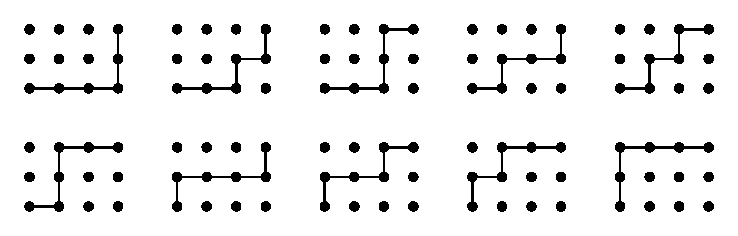
\includegraphics[width=125mm]{img/Gitterwege.pdf}
\caption{Die 10 monotonen Gitterwege von $(0,0)$ nach $(3,2)$.}
\label{fig:Gitterwege}
\end{center}
\end{figure}

\noindent
Kombinatorische Aufgaben tendieren dazu, sich einer bildlichen
Anschauung zu entziehen. Um dem ein wenig entgegenzuwirken, will
ich den folgenden Sachverhalt aufführen, der die Binomialkoeffizienten
mit monotonen Gitterwegen in Beziehung setzt. Als Beispiel listet
Abb. \ref{fig:Gitterwege} jeden der 10 möglichen Wege von Knoten
$(0,0)$ nach Knoten $(3,2)$ auf.

\begin{Satz}
Ein Weg auf dem Gitter $\Z\times\Z$ heiße \emph{monoton}, wenn von $(x,y)$
aus lediglich der Schritt nach $(x+1,y)$ oder der Schritt nach $(x,y+1)$
gewährt ist. Die Anzahl der monotonen Gitterwege von $(0,0)$ nach
$(x,y)$ beträgt
\[\frac{(x+y)!}{x!y!} = \binom{x+y}{x} = \binom{x+y}{y}.\]
\end{Satz}
\begin{Beweis}
Es bezeichne $f(x,y)$ die Anzahl der monotonen Wege von $(0,0)$ nach
$(x,y)$. Zum Erreichen eines Punktes auf den Achsen besteht immer
nur ein möglicher Weg, womit $f(x,0)=1$ und $f(0,y)=1$ gelten muss. Ein
nicht auf den Achsen befindlicher Punkt $(x,y)$ kann von $(x-1,y)$ oder
$(x,y-1)$ aus erreicht werden, was zur Rekurrenz
\[f(x,y) = f(x-1,y) + f(x,y-1)\]
führt. Die Tabellierung der Werte macht ersichtlich, dass sie
ein gedrehtes pascalsches Dreieck erzeugt. Wir setzen daher
$C(x+y,x):=f(x,y)$ und führen die Koordinatentransformation $x+y=n$
und $x=k$ aus. Die Rekurrenz nimmt damit die Form
\[C(n,k) = C(n-1,k-1) + C(n-1,k),\quad C(n,0)=1,\quad C(n,n)=1\]
an, die aber eindeutig den Binomialkoeffizienten charakterisiert.\,\qedsymbol
\end{Beweis}

\noindent
Ein analoger Sachverhalt besteht für Gitter in höheren Dimensionen,
was zum Begriff des \emph{Multinomialkoeffizienten} führt.

Man kann auch eine gruppentheoretische Sichtweise auf die Kombinationen
einnehmen. Die Teilmengen von $Y$ mit $k$ Elementen sind wie Listen, die
jedes der $k$ Elemente genau einmal enthalten. Der Unterschied zu diesen
Listen besteht genau darin, dass es bei den Teilmengen nicht auf die
Reihenfolge der Elemente ankommt. Um die Anzahl der Teilmengen zu
zählen, müssen demzufolge Listen, die sich lediglich durch ihre
Reihenfolge unterscheiden, als äquivalent angesehen werden. Ihre
Äquivalenzklassen stellen somit quasi Listen dar, die die Reihenfolge
ihrer Elemente vergessen haben.

Wir verwenden eine beliebige Menge $X$ mit $|X|=k$ als Indexmenge,
beispielsweise direkt $X:=\{0,\ldots,k-1\}$. Je zwei Listen sind damit
gegeben durch Injektionen $f,g\colon X\to Y$. Die beiden Listen werden
als äquivalent angesehen, sofern sie sich lediglich durch eine
Permutation $\pi$ ihrer Indizes unterscheiden, also
\[f\sim g\,:\Leftrightarrow\,\exists\pi\in S_k\colon f = g\circ\pi.\]
Es sei ferner $\mathrm{Inj}(X,Y)$ die Menge der Injektionen $X\to Y$
und $\mathrm{Inj}(X,Y)/S_k$ die Quotientenmenge bezüglich der
Äquivalenzrelation bzw. der Gruppe $S_k$.
\begin{Satz}\label{Bij-Inj-Teilmengen}
Es sei $C_k(Y)$ die Menge der $k$-elementigen Teilmengen von $Y$.
Zwischen $\mathrm{Inj}(X,Y)/S_k$ und $C_k(Y)$ besteht eine
kanonische Bijektion.
\end{Satz}
\begin{Beweis}
Wir definieren diese Bijektion als
\[\varphi\colon\mathrm{Inj}(X,Y)/S_k\to C_k(Y),\quad\varphi([f]) := f(X),\]
wobei $[f]=f\circ S_k$ die Äquivalenzklasse des Repräsentanten $f$
bezeichne. Die Abbildung $\varphi$ ist wohldefiniert, denn für je zwei $f,g$
mit $f\sim g$ ist eine Permutation $\pi$ vorhanden, so dass gilt
\[f(X) = (g\circ\pi)(X) = g(\pi(X)) = g(X).\]
Zum Nachweis der Injektivität von $\varphi$ muss $[f]=[g]$ aus
$f(X)=g(X)$ gewonnen werden. Gesucht ist also eine Permutation
$\pi$ mit $f=g\circ\pi$. Weil $g$ injektiv ist, existiert eine
Linksinverse $g^{-1}$, so dass $\pi := g^{-1}\circ f$ gewählt werden
kann. Es verbleibt die Gleichheit $f = g\circ g^{-1}\circ f$ zu
bestätigen. Zwar ist $g^{-1}$ im Allgemeinen keine Rechtsinverse von $g$,
ihre Einschränkung auf $g(X)$ aber schon. Wegen $f(X)=g(X)$ hebt sich
$g\circ g^{-1}$ daher auf $f(X)$ weg.

Zur Surjektivität von $\varphi$. Hier ist zu zeigen, dass es zu jeder
Menge $B\in C_k(Y)$ eine Injektion $f\colon X\to Y$ mit $f(X)=B$ gibt.
Weil $X$ und $B$ gleichmächtig sind, existiert eine Bijektion $f_0\colon X\to B$,
womit man die gesuchte Injektion mit der Setzung $f(x):=f_0(x)$ erhält.\,\qedsymbol
\end{Beweis}

\noindent
Bezüglich $|X|=k$ tut sich nun die Umformung
\[|C_k(Y)| \stackrel{\text{(1)}}= |\mathrm{Inj}(X,Y)/S_k|
\stackrel{\text{(2)}}= \frac{|\mathrm{Inj}(X,Y)|}{|S_k|} =
\frac{n^{\underline k}}{k!} = \binom{n}{k}\]
auf. Der Schritt (1) wurde bereits durch Satz
\ref{Bij-Inj-Teilmengen} abgeklärt. Die Einsicht in (2) erhält man
folgendermaßen. Für jede Gruppe $G$ gilt die Bahnformel
$|G| = |f\circ G|\cdot |G_f|$. Bei trivialer Fixgruppe $G_f$ gilt
$|G_f| = 1$, mithin $|f\circ G| = |G|$. Namentlich bei der symmetrischen
Gruppe $G=S_k$ tritt dieser Umstand ein. Aus diesem Grund enthält jede
Bahn $f\circ S_k$ gleich viele Elemente, $|S_k|$ an der Zahl. Weil
die Bahnen außerdem paarweise disjunkt sind, ergibt sich deshalb
die Faktorisierung
\[|\mathrm{Inj}(X,Y)| = |S_k|\cdot |\mathrm{Inj}(X,Y)/S_k|.\]
Der gemachte Gedankengang kann auch unter anderen Umständen vorgenommen
werden, dergestalt dass statt den Injektionen die Surjektionen oder sämtliche
Abbildungen betrachtet werden. Es entsteht der \emph{zwölffaltige Weg},
-- wenn man so will, ein kleines Periodensystem der Kombinatorik, 
siehe Tabelle \ref{tab:twelvefold-way}. \cite{Stanley}

\begin{table}
\begin{center}
\caption{Der zwölffaltige Weg}
\label{tab:twelvefold-way}
\begin{tabular}{c|ccc}
\toprule
& $f\in\Abb(X,Y)$ & $f\in\mathrm{Inj}(X,Y)$ & $f\in\mathrm{Sur}(X,Y)$\\
\midrule[\heavyrulewidth]
$f$ & $n^k$ & $n^{\underline k}$ & $n!\big\{\!\begin{smallmatrix}k\\ n\end{smallmatrix}\!\big\}$\\[4pt]
$f\circ S_k$ & $\big(\!\begin{smallmatrix}n+k-1\\ k\end{smallmatrix}\!\big)$
& $\big(\!\begin{smallmatrix}n\\ k\end{smallmatrix}\!\big)$
& $\big(\!\begin{smallmatrix}k-1\\ k-n\end{smallmatrix}\!\big)$\\[4pt]
$S_n\circ f$ & $\sum_{i=0}^n \big\{\!\begin{smallmatrix}k\\ i\end{smallmatrix}\!\big\}$
& $[k\le n]$ & $\big\{\!\begin{smallmatrix}k\\ n\end{smallmatrix}\!\big\}$\\[4pt]
$S_n\circ f\circ S_k$ & $p_n(n+k)$ & $[k\le n]$ & $p_n(k)$\\
\bottomrule
\end{tabular}
\end{center}
\end{table}

Der Term $\big\{\!\begin{smallmatrix}k\\ n\end{smallmatrix}\!\big\}$
steht dabei für die Stirlingzahlen zweiter Art, das ist die Anzahl der
Möglichkeiten, wie eine Menge von $k$ Elementen in $n$ disjunkte nichtleere
Teilmengen zerlegt werden kann. Der Term $p_n(k)$ steht für die Anzahl
der Partitionen der Zahl $k$ in $n$ Teile. Der Term $[k\le n]$ steht
für »$1$, falls $k\le n$, sonst $0$«.

\subsection{Anzahl der Multimengen}

Aus der Frage nach der Anzahl Kombinationen geht als abgewandelte
Problemstellung die Frage nach der Anzahl Kombinationen mit
Wiederholung einher. Das heißt, während bei einer Kombination von
$k$ aus $n$ unterschiedlichen Objekten jedes der $k$ Objekte höchstens
einmal auftreten darf, kann bei einer Kombination mit Wiederholung
jedes der $n$ Objekte beliebig häufig, also bis zu $k$ mal auftreten.
Während eine Kombinationen eine Menge von $k$ aus einer Menge von $n$
Elementen darstellt, handelt es sich bei einer Kombination mit
Wiederholung um eine Multimenge von $k$ aus der Menge von $n$ Elementen.

Eine gute Veranschaulichung bietet die folgende Aufgabe.
Aus einem Sack mit unerschöpflich vielen Bauklötzen der Farben rot, grün,
blau und gelb werden gleichzeitig fünf Stück gezogen. Zur Frage steht,
wie viele unterschiedliche Farbkombinationen es gibt.

\begin{figure}\setlength{\abovecaptionskip}{0pt}
\begin{center}
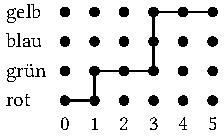
\includegraphics[width=38mm]{img/Kloetze.pdf}
\caption{Eine Kombination von fünf Klötzen in bis zu vier Farben.}
\label{fig:Kloetze}
\end{center}
\end{figure}

Diese Aufgabe kann als die Frage nach der Anzahl monotoner Gitterwege
umgedeutet werden. Ein Schritt nach rechts fügt dabei einen Klotz zur
Sammlung hinzu. Ein Schritt nach oben wechselt dagegen in die nächste Farbe,
ohne die bisherige Sammlung von Klötzen zu vergrößern.
Siehe Abb. \ref{fig:Kloetze}. Es stellt sich heraus, dass sich diese Sichtweise
zur Methodik \emph{Stars and Bars} gleichbedeutend verhält. Dabei wird
ein Sternchen für einen Klotz gesetzt und ein Stab als Abgrenzung
zwischen zwei Farben. Man setzt ein Sternchen also gerade für einen
Schritt nach rechts und einen Stab suggestiv für einen Schritt
nach oben.

Man muss hier vorsichtig sein, keinen Off-by-one-Fehler zu machen.
Zwar gibt es vier Farben, diese werden allerdings mit $0$, $1$, $2$, $3$
nummeriert. Eine Sammlung von $k$ Klötzen aus einem Sack mit $n$ Farben
entspricht also einem Gitterweg von $(0,0)$ zu $(k,n-1)$. Die Anzahl
der Farbkombinationen beträgt somit
\[\left(\!\left(\begin{matrix}n\\ k\end{matrix}\right)\!\right) :=
\binom{k+n-1}{k} = \binom{k+n-1}{n-1} = \binom{5+4-1}{4-1} = \binom{8}{3} = 56.\]
Das doppelt geklammerte Analogon zum Binomialkoeffizienten wird also als
die Anzahl der $k$-elementigen Multimengen mit Elementen aus einer Menge
von $n$ Elementen interpretiert. Wie es scheint, stimmt sie mit der Anzahl
der $k$-elementigen Teilmengen aus einer Menge von $k+n-1$ Elementen
überein.

\subsection{Gesamtzahl der Teilmengen}

Die Zählung der Teilmengen beschränkte sich zuvor auf Teilmengen fester
Größe. Nun würden wir gerne auch in Erfahrung bringen, wie viele mögliche
Teilmengen einer Menge $M$ es insgesamt gibt, also wie groß die
Potenzmenge von $M$ ist.

Zunächst kurz ein leichter Hilfssatz.

\begin{Satz}\label{ohne-ist-monoton}
Aus $A\subseteq B$ folgt $A\setminus C\subseteq B\setminus C$.
\end{Satz}
\begin{Beweis}
Es gelte $x\in A\setminus C$. Das bedeutet, $x\in A$ und $x\notin C$.
Laut der Voraussetzung folgt $x\in B$ aus $x\in A$. Somit gilt sowohl
$x\in B$ als auch $x\notin C$, also $x\in B\setminus C$.\,\qedsymbol
\end{Beweis}

\noindent
Als nächstes klären wir die Rekurrenz der Potenzmengenoperation ab,
die daraufhin in einem Induktionsbeweis Verwendung findet. Auf Basis
ihrer lässt sich außerdem ein Algorithmus zur Aufzählung der Potenzmenge
erstellen.

\begin{Satz}[Rekurrenz der Potenzmengenoperation]%
\label{Potenzmenge-rekursiv}\newlinefirst
Für $x\notin M$ gilt $\powerset(M\cup\{x\})
= \powerset(M)\cup\{A\cup\{x\}\mid A\in\powerset(M)\}$.
\end{Satz}
\begin{Beweis}
Die Gleichung ist äquivalent zu
\[T\subseteq M\cup\{x\}\,\Leftrightarrow\, T\subseteq M\lor\exists A\subseteq M\colon T=A\cup\{x\}.\]
Die rechte Seite gelte. Im Fall $T\subseteq M$ gilt erst
recht $T\subseteq M\cup\{x\}$. Im anderen Fall liegt ein $A\subseteq M$
vor, womit $A\cup\{x\}\subseteq M\cup\{x\}$ gilt. Wegen $T=A\cup\{x\}$
gilt also ebenfalls $T\subseteq M\cup\{x\}$.

Die linke Seite gelte. Mit $T\subseteq M\cup\{x\}$ und
$x\notin M$ folgt per Satz \ref{ohne-ist-monoton}
\[T\setminus\{x\}\subseteq (M\cup\{x\})\setminus\{x\} = M,
\;\text{also}\; T\setminus\{x\}\subseteq M.\]
Im Fall $x\notin T$ ist
$T=T\setminus\{x\}$, womit man $T\subseteq M$
erhält. Im gegenteiligen Fall $x\in T$ wird $A:=T\setminus\{x\}$
als Zeuge der Existenzaussage gewählt.\,\qedsymbol
\end{Beweis}

\noindent
Es verhält sich dergestalt, dass \emph{sämtliche} in der Rekurrenz
auftretende Vereinigungen solche disjunkter Mengen sind. Man darf
die Rekurrenz somit auch als
\[\powerset(M\uplus\{x\})
= \powerset(M)\uplus\biguplus_{\mathclap{A\in\powerset(M)}}
\{A\uplus\{x\}\}\]
notieren. Nun zur gesuchten Anzahl.

\begin{Satz}\label{Anzahl-Potenzmenge}
Mit $|M|=n$ gilt $|\powerset(M)| = 2^n$.
\end{Satz}
\begin{Beweis}
Induktion über $n$. Im Anfang $n=0$ muss $M=\emptyset$ sein, also
$\powerset(M)=\{\emptyset\}$, das macht $|\powerset(M)| = 1 = 2^0$.

Zum Schritt. Es gelte $|M|=n$ und es sei $x\notin M$. Vermittels Satz
\ref{Potenzmenge-rekursiv}, wo man es außerdem mit Vereinigungen
disjunkter Mengen zu tun hat, erhält man
\[|\powerset(M\cup\{x\})| = |\powerset(M)| + |\{A\cup\{x\}\mid A\in\powerset(M)\}|
\stackrel{\text{IV}}= 2^n + 2^n = 2^{n+1}.\,\qedsymbol\]
\end{Beweis}

\noindent
Einen kürzeren Beweis erhalten wir, wenn ihr uns daran erinnern, dass
$\powerset(M)$ und $\Abb(M,\{0,1\})$ gleichmächtig sind. Demnach gilt
\[|\powerset(M)| = |\Abb(M,\{0,1\})| = |\{0,1\}|^{|M|} = 2^{|M|}.\]
Als Korollar ergibt sich kurzerhand die Beziehung
\[\sum_{k=0}^n\binom{n}{k} = 2^n,\]
denn summiert man die Anzahl der $k$"=elementigen Teilmengen über $k$,
erhält man die Anzahl sämtlicher Teilmengen einer Menge von $n$ Elementen.
Und führt man einen unabhängigen Induktionsbeweis dieser Beziehung,
erhält man umgekehrt einen dritten Beweis von Satz \ref{Anzahl-Potenzmenge}.

\newpage
\section{Zur elementaren Zahlentheorie}

\subsection{Kongruenzen}

Die elementare Zahlentheorie beschäftigt sich mit der Teilbarkeit von
Zahlen, den Resten, die bei der Ganzzahldivision übrig bleiben
und der Auffindung ganzzahliger Lösungen von Gleichungen. Lange Zeit
als ein Gebiet der reinen Mathematik angesehen, stellte sie sich
als bedeutsam für die praktische Informatik und die Kryptologie heraus. 

Die \emph{modulare Arithmetik}, auch \emph{Restklassenarithmetik}
genannt, ist ein wichtiges Hilfsmittel der elementaren Zahlentheorie.
Sie geht aus der gewöhnlichen Arithmetik hervor, indem zwei ganze
Zahlen als gleich angesehen werden, wenn sie bei Division durch eine
vorab gewählte feste Zahl denselben Rest lassen. Diese Form der
Gleichheit nennt man \emph{Kongruenz}, die feste Zahl den \emph{Modul}.
Kongruenz zweier Zahlen ist damit gleichbedeutend, dass die eine
Zahl zur anderen um ein Vielfaches des Moduls verschoben liegt, was nichts
anderes bedeutet, als dass der Modul die Differenz der beiden Zahlen teilt.

Man vermittelt das Konzept gern am Lauf von Uhrzeigern. Hierbei werden
die Stunden $0, 12, 24, 36$ usw. als gleich angesehen. Entsprechend
werden die Stunden $1, 13, 25, 37$ usw. als gleich angesehen. Es
verbleiben nur noch $12$ unterschiedliche Zeitpunkte, die vollen
Stunden $0, 1, \ldots, 11$. Ein Uhrzeiger auf $11$ Uhr trifft
zwei Stunden später auf $1$ Uhr. Anders ausgedrückt sind die Zahlen
$11+2$ und $1$ kongruent Modulo 12, was nach Carl Friedrich Gauß
in der Form
\[11 + 2\equiv 1\pmod{12}\]
notiert wird.

\begin{Definition}[Kongruenz]\index{Kongruenz}\newlinefirst
Zwei ganze Zahlen $a,b$ heißen kongruent modulo $m$, wenn ihre Differenz
$a-b$ durch $m$ teilbar ist,%
\[a\equiv b\pmod{m}\;:\bicond\;\exists k\in\Z\colon a-b=km.\]
\end{Definition}
Statt »$(\mathrm{mod}\;m)$« schreibt man beim Rechnen meist
kürzer »$(m)$«.

\begin{Satz}
Die Kongruenz ist eine Äquivalenzrelation, das heißt, es gilt
\begin{align*}
&a\equiv a\pmod{m},&&\text{(Reflexivität)}\\
&a\equiv b\cond b\equiv a\pmod{m},&&\text{(Symmetrie)}\\
&a\equiv b\land b\equiv c\cond a\equiv c\pmod{m}.&&\text{(Transitivität)}
\end{align*}
\end{Satz}
\begin{Beweis}
Für die Reflexivität ist ein $k$ mit $0=a-a=km$
zu finden. Setze $k=0$.

Bei der Symmetrie gibt es nach Voraussetzung
ein $k$ mit $a-b=km$. Dann ist $b-a=-km$. Setze $k'=-k$.
Es gibt also $k'$ mit $b-a=k'm$, somit gilt $b\equiv a$.

Bei der Transitivität gibt es nach Voraussetzung ein $k$ mit
$a-b=km$ und ein $l$ mit $b-c=lm$. Das heißt, es gilt
$km+lm = a-c$, \text{ergo} $a-c = (k+l)m$. Setze $k'=k+l$. Es gibt also
$k'$ mit $a-c=k'm$. Somit gilt $a\equiv c$.\;\qedsymbol
\end{Beweis}

\begin{Satz}\label{Kongruenz-add-sub}
Sind $a,b,c$ ganze Zahlen, dann gilt
\begin{align*}
a\equiv b\pmod{m}&\iff a+c\equiv b+c\pmod{m},\\
a\equiv b\pmod{m}&\iff a-c\equiv b-c\pmod{m}.
\end{align*}
\end{Satz}
\begin{Beweis}
Unter Beachtung von $(b+c)-(a+c)=b-a$ findet man
\begin{gather*}
a\equiv b\pmod{m}
\iff (\exists k\in\Z\colon b-a=km)\\
\iff (\exists k\in\Z\colon (b+c)-(a+c)=km)\\
\iff a+c\equiv b+c\pmod{m}.
\end{gather*}
Für die Subtraktion von $c$ ist die Überlegung analog.\;\qedsymbol
\end{Beweis}

%\newpage
\begin{Satz}\label{Kongruenz-mul}
Sind $a,b,c$ ganze Zahlen, dann gilt
\[a\equiv b\pmod{m} \implies ac\equiv bc\pmod{m}.\]
\end{Satz}
\begin{Beweis}
Unter der Voraussetzung $a\equiv b\pmod{m}$ gibt es ein
$k$ mit $b-a=km$. Es gilt
\[b-a=km\iff (b-a)c=kcm \iff bc-ac=k'm\]
mit $k':=kc$. Man hat also
\[(\exists k'\in\Z\colon bc-ac=k'm)\iff ac\equiv bc\pmod{m}.\;\qedsymbol\]
\end{Beweis}

\begin{Satz}
Gilt $a\equiv a'\pmod{m}$ und
$b\equiv b'\pmod{m}$, dann gilt auch
\begin{align*}
a+b&\equiv a'+b'\pmod{m},\\
a-b&\equiv a'-b'\pmod{m},\\
ab&\equiv a'b'\pmod{m}.
\end{align*}
\end{Satz}
\strong{Beweis.} Man findet
\[\left.\begin{aligned}
a\equiv a'&\implies a+b\equiv a'+b\\
b\equiv b'&\implies a'+b\equiv a'+b'
\end{aligned}\right\}
\implies a+b\equiv a'+b\equiv a'+b'\pmod{m}.\]
Für die Subtraktion ist die Überlegung analog. Für die Multiplikation
ebenfalls:%
\[\left.\begin{aligned}
a\equiv a'&\implies ab\equiv a'b\\
b\equiv b'&\implies a'b\equiv a'b'
\end{aligned}\right\}
\implies ab\equiv a'b\equiv a'b'\pmod{m}.\;\qedsymbol\]

\begin{Satz}
Addition des Moduls führt auf eine kongruente Zahl:%
\[a\equiv a+m\equiv a-m\pmod{m}.\]
\end{Satz}
\begin{Beweis}
Es gilt
\[a\equiv a+m\pmod{m}\iff (\exists k\in\Z\colon km=(a+m)-a=m).\]
Setze $k=1$. Bei
\[a\equiv a-m\pmod{m}\iff (\exists k\in\Z\colon km=(a-m)-a=-m)\]
setze $k=-1$.\;\qedsymbol
\end{Beweis}

\subsection{Teilbarkeit}

Die Beziehung »$m$ teilt $a$« ist definiert als
\[m\mid a\defiff (\exists k\in\Z\colon a=km) \iff a\equiv 0\pmod{m}.\]
Während die Kongruenz eine Äquivalenzrelation ist, stellt die
Teilbarkeit eine Halbordnung dar, dergestalt dass sie die drei Axiome
\begin{align*}
&\forall a\in\Z\colon a\mid a, &&\text{(Reflexivität)}\\
&\forall a,b\in\Z\colon a\mid b\land b\mid a\cond a = b,&&\text{(Antisymmetrie)}\\
&\forall a,b,c\in\Z\colon a\mid b\land b\mid c\cond a\mid c.&&\text{(Transitivität)}
\end{align*}
erfüllt. Teilt $a$ die Zahl $b$, ist $a$ also in gewisser Weise kleiner
als $b$.

\subsection{Restklassenringe}

Wir könnten nun beginnen, mit der modularen Arithmetik interessante
Probleme zu lösen. Zunächst möchte ich aber erläutern, wie die
modulare Arithmetik mit dem Restklassenring zusammenhängt. Unter
diesem Blickwinkel bekommen wir ein tieferes Verständnis und können
Mittel der Ringtheorie und Gruppentheorie anwenden.

Zu einer ganzen Zahl $a$ ist die Restklasse modulo $m$ definiert als 
\[[a]_m := \{x\mid x\equiv a\pmod m\}.\]
Eine alternative Schreibweise für $[a]_m$ ist $a+m\Z$. Weil die
Kongruenz eine Äquivalenzrelation ist, handelt es sich bei den
Restklassen um Äquivalenzklassen. Wir betrachten nun die
Quotientenmenge
\[\Z/m\Z := \{[a]_m\mid a\in\Z\}.\]
Nun können wir die Addition und Multiplikation von Restklassen
definieren.
\begin{Satz}
Auf $\Z/m\Z$ sind die beiden Operationen
\begin{align*}
[a]_m + [b]_m &:= [a+b]_m,\\
[a]_m\cdot [b]_m &:= [ab]_m
\end{align*}
wohldefiniert.
\end{Satz}
\strong{Beweis.} Zu zeigen ist, dass $a+b\equiv x+y$ gilt, sofern
$a\equiv x$ und $b\equiv y$ ist. Gemäß Satz \ref{Kongruenz-add-sub} gilt
\begin{align*}
a\equiv x &\iff a+b\equiv x+b,\\
b\equiv y &\iff x+b\equiv x+y.
\end{align*}
Aus den beiden Prämissen erhalten wir demzufolge
$a+b\equiv x+b\equiv x+y$.
Die Argumentation zur Multiplikation ist analog, wobei
Satz \ref{Kongruenz-mul} zur Anwendung kommt.\,\qedsymbol

Die Struktur $(\Z/m\Z,+,\cdot)$ nennt man den \emph{Restklassenring}
zum Modul $m$.

\begin{Satz}
Jeder Restklassenring ist ein kommutativer unitärer Ring.
\end{Satz}
\begin{Beweis}
Bereits bewiesen wurde, dass die ganzen Zahlen einen
kommutativen unitären Ring bilden. Aufgrund der Wohldefiniertheit der
Addition und Multiplikation ist Kongruenz modulo $m$ eine
Kongruenzrelation. Satz \ref{Kongruenz-Ring-Quotient} zeigt somit die
Behauptung.\,\qedsymbol
\end{Beweis}

\noindent
Zudem ist die Quotientenabbildung
\[\varphi\colon\Z \to \Z/m\Z,\quad \varphi(a):=[a]_m.\]
ein Eins-erhaltender Ringhomomorphismus, wie aus dem Beweis
von Satz \ref{Kongruenz-Ring-Quotient} hervorgeht.

%\newpage
\subsection{Euklidische Division}

\begin{Satz}[Lemma zur euklidischen Division]\mbox{}\\*
Zu je zwei ganzen Zahlen $a,b$ mit $b\ne 0$ gibt es zwei eindeutig
bestimmte Zahlen $q,r$ mit $0\le r<|b|$, so dass $a=bq+r$. Man nennt
$q$ den \emph{Quotient} und $r$ den \emph{Rest}.
\end{Satz}
\begin{Beweis}[Beweis der Existenz]
Betrachten wir zunächst den Fall, bei dem $a\ge 0$
und $b>0$ ist. Man kann dann sooft $b$ von $a$ abziehen, bis sich eine
Zahl $\ge 0$ und $<b$ ergibt. Formal bilden wir die
Folge $r_k := a-bk$. Nun muss für irgendein $k\ge 0$ schließlich
$0\le r_k<b$ sein. Damit ist $q=k$ und $r=r_k$ gefunden.

Sei nun $a<0$. Wie bereits gezeigt gibt es $q,r$ mit $-a = bq+r$.
Für $r=0$ haben wir dann mit $q':=-q$ und $r':=0$ einen Quotient
und einen Rest. Sei nun $r\ne 0$. Dann gilt
\[a = -bq-r = -(q+1)b + b - r.\]
Mit $q':=-(q+1)$ und $r':=b-r$ gibt es somit auch in diesem Fall einen
Quotient und einen Rest. Der Rest erfüllt auch die gewünschte
Ungleichung, denn aus $r<b$ ergibt sich $0<r'$ und aus $0<r$ ergibt
sich $r'<b$.

Sei nun $a$ beliebig und $b<0$. Dann gibt es $q,r$ mit $a=(-b)q+r$.
Setze also $q':=-q$ und $r':=r$. Damit gilt $a=bq'+r'$, womit
auch in diesem Fall ein Quotient und ein Rest gefunden ist.\,\qedsymbol
\end{Beweis}
\begin{Beweis}[Beweis der Eindeutigkeit]
Das Paar $q,r$ erfülle
$a=bq+r$ und $q',r'$ erfülle ebenfalls $a=bq'+r'$. Dann gilt
\[bq+r = bq'+r',\iff b(q-q') = r'-r,\implies |b| |q-q'| = |r'-r|.\]
Aus $0<r<|b|$ und $0<r'<|b|$ erhält man außerdem $|r'-r|<|b|$. Somit
muss $|b| |q-q'| < |b|$ sein, also $|q-q'| < 1$. Eine nichtnegative
ganze Zahl kann aber nur dann kleiner als eins sein, wenn sie null
ist. Damit hat man
\[|q-q'|=0,\iff q-q'=0,\iff q=q'.\]
Entsprechend folgt $r=r'$.\,\qedsymbol
\end{Beweis}

Bei der euklidischen Division $a:b$ ist $(a\bmod b)$ eine geläufige
Schreibweise für den Rest. Das Lemma zur euklidischen Division sagt uns,
dass jede Restklasse von $\Z/m\Z$ einen kanonischen Repräsentant
besitzt. Nämlich besitzt die Restklasse $[a]_m$ den kanonischen
Repräsentant $r=(a\bmod m)$, denn $a=mq+r$ bedeutet dass $a-r$ durch
$m$ teilbar ist, also
\[a\equiv r\pmod m,\quad\text{bzw.}\quad [a]_m = [r]_m.\]


\subsection{Rundung}

Manche Formeln oder Rechnungen verlangen das Runden von Zahlen auf
eine ganze Zahl oder auf eine bestimmte Zahl von Nachkommastellen.
Im Algorithmus, der Vektorgrafiken als Rastergrafik aus Pixeln rendern
soll, muss zum Beispiel zwangsläufig an irgendeiner Stelle gerundet
werden. Außerdem ist Runden in vielen händischen Rechnungen
allgegenwärtig, sei es in wissenschaftlichen, technischen, gewerblichen
oder alltäglichen.

Als nächstes will ich daher erklären, wie Funktionen zum Runden formal
definiert werden, und welche Eigenschaften sie besitzen. Als wichtige
Grundfunktionen treten dabei die \emph{Abrundungsfunktion}, engl.
\emph{floor}, und die \emph{Aufrundungsfunktion}, engl. \emph{ceil},
auf, die vereinzelt auch in der Kombinatorik und in der Zahlentheorie
vorkommen.

\begin{Definition}[Floor]\label{def:floor}\index{Floorfunktion}
Für $x\in\R$ definiert man
\[y = \lfloor x\rfloor\,:\Leftrightarrow\, y\in\Z\land 0\le x-y < 1.\]
\end{Definition}

\begin{Definition}[Ceil]\label{def:ceil}\index{Ceilfunktion}
Für $x\in\R$ definiert man
\[y = \lceil x\rceil\,:\Leftrightarrow\, y\in\Z\land 0\le y-x < 1.\]
\end{Definition}

\begin{Satz}\label{floor-add-int}
Für jede ganze Zahl $k$ gilt $\lfloor k + x\rfloor = k + \lfloor x\rfloor$.
\end{Satz}
\begin{Beweis} Aufgrund der Prämisse $k\in\Z$ ist $y\in\Z$ äquivalent
zu $y-k\in\Z$. Unter dieser Gegebenheit findet sich mit
Def. \ref{def:floor} die äquivalente Umformung
\begin{align*}
y = \lfloor k+x\rfloor &\iff y\in\Z\land 0\le (k+x)-y < 1\\
&\iff y-k\in\Z\land 0\le x-(y-k) < 1\\
&\iff y - k = \lfloor x\rfloor \iff y = k + \lfloor x\rfloor.\,\qedsymbol
\end{align*}
\end{Beweis}

\begin{Satz}\label{floor-is-zero}
Für $0\le x < 1$ gilt $\lfloor x\rfloor = 0$.
\end{Satz}
\begin{Beweis}
Dies folgt unmittelbar aus Def. \ref{def:floor}.\,\qedsymbol
\end{Beweis}

\begin{Satz}
Es gilt
\[\begin{array}{@{}l@{\,}c@{\,}c@{}l@{\,}c@{\,}c@{}l}
\lfloor x\rfloor &=& \max &\{k\in\Z\mid k\le x\} &=& \min &\{k\in\Z\mid x < k + 1\},\\[2pt]
\lceil x\rceil &=& \min &\{k\in\Z\mid x\le k\} &=& \max &\{k\in\Z\mid k - 1 < x\}.
\end{array}\]
\end{Satz}
\begin{Beweis}
Mit bezüglich $y=\lfloor x\rfloor$ entfalteten Def. \ref{def:floor},
\ref{def:max-min} lautet die Aussage
\[y\in\Z\land 0\le x-y<1\iff
y\in\Z\land y\le x\land (\forall k\in\Z\colon k\le x\Rightarrow k\le y).\]
Für die Implikation von links nach rechts ist im Wesentlichen
\[k\in\Z, y\in\Z, k\le x, x < y+1\vdash k\le y\]
zu zeigen. Man erhält zunächst $k < y+1$ per Transitivgesetz.
Wegen $k,y\in\Z$ folgt daraus $k\le y$. Für die Implikation von rechts
nach links ist im Wesentlichen
\[y\in\Z,(\forall k\in\Z\colon k\le x\Rightarrow k\le y)\vdash x < y + 1\]
zu zeigen. Angenommen, es wäre $y+1\le x$. Die Allaussage wird mit
$k:=y+1$ spezialisiert. Per Modus ponens erhält man den Widerspruch
$y+1\le y$. Ergo muss die Annahme falsch sein, was äquivalent zu
$x<y+1$ ist. Die restlichen Beweise verlaufen analog.\,\qedsymbol
\end{Beweis}

\begin{Satz}\label{floor-div-floor}
Für $x\in\R$ und $n\in\Z_{\ge 1}$ gilt
\[\left\lfloor\frac{x}{n}\right\rfloor
= \left\lfloor\frac{\lfloor x\rfloor}{n}\right\rfloor.\]
\end{Satz}
\begin{Beweis}
Sei $a:=x-\lfloor x\rfloor$. Per Def. \ref{def:floor} gilt $0 \le a < 1$.
Laut dem Lemma zur euklidischen Division gilt außerdem
$\lfloor x\rfloor = qn+r$
mit $q=\lfloor\frac{\lfloor x\rfloor}{n}\rfloor$
und $0\le r\le n - 1$. Infolge gilt $0\le a+r<n$, also
$0\le\frac{a+r}{n}<1$ und somit $\lfloor\frac{a+r}{n}\rfloor = 0$
laut Satz \ref{floor-is-zero}.
Es findet sich%
\[\left\lfloor\frac{x}{n}\right\rfloor
= \left\lfloor\frac{a+\lfloor x\rfloor}{n}\right\rfloor
= \left\lfloor\frac{a+qn+r}{n}\right\rfloor
\stackrel{\text{(1)}}= q + \left\lfloor\frac{a+r}{n}\right\rfloor
\stackrel{\text{(2)}}= q =
\left\lfloor\frac{\lfloor x\rfloor}{n}\right\rfloor,\]
wobei (1) laut Satz \ref{floor-add-int} gilt, und (2)
wie soeben ausgeführt.\,\qedsymbol
\end{Beweis}

\begin{Satz}
Für $x\in\R$ und $m,n\in\Z$ mit $n\ge 1$ gilt
\[\left\lfloor\frac{m+x}{n}\right\rfloor
= \left\lfloor\frac{m+\lfloor x\rfloor}{n}\right\rfloor.\]
\end{Satz}
\begin{Beweis}
Laut Satz \ref{floor-add-int} ist $m+\lfloor x\rfloor = \lfloor m+x\rfloor$.
Die Aussage folgt nun als Korollar aus Satz \ref{floor-div-floor}.\,\qedsymbol
\end{Beweis}

\noindent
Das Runden einer Zahl auf eine ganze Zahl kann vermittels floor als
\[\mathrm{round}(x) := \mathrm{sgn}(x)\lfloor |x|+\tfrac{1}{2}\rfloor\]
beschrieben werden. Das Runden auf die $n$-te Nachkommastelle daraufhin als
\[\mathrm{round}(x, n) := \frac{\mathrm{round}(10^n x)}{10^n}.\]


\chapter{Elemente der Stochastik}

\section{Grundbegriffe}

\subsection{Ereignisse}

Die Wahrscheinlichkeitstheorie beschäftigt sich mit
\emph{Zufallsexperimenten}. Darunter versteht man ein Experiment
mit zufälligem Ausgang, das, um der Wissenschaftlichkeit genüge zu tun,
unter genau definierten Versuchsbedingungen durchgeführt wird.
Der Ausgang führt immer zu einem \emph{Ergebnis}. Alle erreichbaren
Ergebnisse fasst man zur \emph{Ergebnismenge} zusammen. Allgemeiner
genügt es, wenn jedes Ergebnis in der Ergebnismenge liegt, wobei diese
aber auch Elemente enthalten darf, die das Experiment niemals abwirft.
Jede Teilmenge der Ergebnismenge nennt man ein \emph{Ereignis}\index{Ereignis}.
Die Potenzmenge der Ergebnismenge heißt \emph{Ereignisraum}, sie
besteht aus allen denkbaren Ereignissen. Man sagt, ein Ereignis sei
eingetreten, wenn das Ergebnis des Versuchs im diesem Ereignis liegt.

Zu beachten ist, dass wir dabei eine endliche oder höchstens
abzählbar unendliche Ergebnismenge voraussetzen. Bei überabzählbaren
Ergebnismengen kommt es zu Unwägbarkeiten, deren Klärung Gegenstand der
Maßtheorie ist.

Ein schlichtes Experiment bietet der Wurf des Spielwüfels, ein mit
Augenzahlen beschriftetes regelmäßiges Hexaeder. Die Ergebnismenge
wird als
\[\Omega := \{1, 2, 3, 4, 5, 6\}\]
festgelegt. Betrachten wir die drei Ereignisse
\[A := \{2\},\quad B := \{1,2\},\quad C:=\{1,3\}.\]
Ist $\omega=2$ das Ergebnis des Versuchs, sind die Ereignisse $A,B$
eingetreten. Zwei Ereignisse, die niemals gleichzeitig eintreten,
heißen \emph{disjunkt}. So sind die $A,C$ disjunkt, weil ihre
Schnittmenge leer ist.

\subsection{Wahrscheinlichkeiten}

Man kann nicht voraussagen, wie ein Experiment ausgehen wird. Das
Wahrscheinlichkeitsmaß liefert dennoch ein Maß dafür, wie sicher der
Eintritt eines Ereignisses ist. Wahrscheinlichkeit wird tiefergründig
verständlich, wenn dasselbe Zufallsexperiment abermals wiederholt wird.
Wir zählen, wie häufig ein Elementarereignis eingetreten ist.

Es sei ein Versuch $n$ mal durchgeführt worden, was zu den Ergebnissen
$a_i$ für $i=1$ bis $i=n$ geführt hat. Wir definieren die \emph{relative
Häufigkeit} des Ereignisses $A$ als die Zahl
\[r_{n,a}(A) := \frac{1}{n}|\{i\in\{1,\ldots,n\}\mid a_i\in A\}|.\]
Relative Häufigkeiten bieten bei hinreichend großem $n$ eine Näherung
für die Wahrscheinlichkeit. Zur Vermessung eines Würfels wird man
diesen also möglichst oft werfen wollen. Man erhält so die relativen
Häufigkeiten der Elementarereignisse, und damit näherungsweise auch
ihre Wahrscheinlichkeiten. So lässt sich feststellen, ob ein
Würfel gezinkt wurde.

Fassen wir $a$ als Funktion $i\mapsto a_i$ auf, können wir schreiben
\[\{i\mid a_i\in A\} = \{i\mid i\in a^{-1}(A)\} = a^{-1}(A).\]
Für disjunkte Ereignisse $A,B$ erhält man nun
\begin{align*}
r_{n,a}(A\cup B) &= \tfrac{1}{n}|a^{-1}(A\cup B)|
= \tfrac{1}{n}|a^{-1}(A)\cup a^{-1}(B)|\\
&= \tfrac{1}{n}|a^{-1}(A)| + \tfrac{1}{n}|a^{-1}(B)|
= r_{n,a}(A) + r_{n,a}(B).
\end{align*}

\subsection{Zufallsgrößen}

Eine \emph{Zufallsgröße}\index{Zufallsgroesse@Zufallsgröße} darf man
sich als eine Funktion $X\colon\Omega\to\Omega'$
vorstellen, die eine kausale Verbindung zwischen den Ergebnismengen
$\Omega,\Omega'$ schafft. Ein Ergebnis $\omega\in\Omega$ führt
zu $X(\omega)$. Ursächlich für ein $x\in\Omega'$ sind daher all die
$\omega$ mit $x=X(\omega)$. Das heißt, ursächlich für das
Elementarereignis $\{x\}$ ist dessen Urbild $X^{-1}(\{x\})$.
Infolge muss die Wahrscheinlichkeit von $\{x\}$ die es Urbildes sein.
Insofern definiert man auf $\Omega'$ das Wahrscheinlichkeitsmaß%
\[P_X\colon\mathcal P(\Omega')\to [0,1],\quad P_X(A) := P(X^{-1}(A)).\]
Man nennt $P_X$ die \emph{Verteilung}\index{Verteilung} von $X$. Mit der
identischen Zufallsgröße
\[\id\colon\Omega\to\Omega,\quad \id(\omega) := \omega\]
versteht sich auch das ursprüngliche Maß $P$ als die Verteilung $P=P_{\id}$.

Geläufig sind die Schreibweisen
\begin{align*}
P(X=x) &:= P(X^{-1}(\{x\})), & \{X=x\} &:= X^{-1}(\{x\}),\\
P(X\in A) &:= P(X^{-1}(A)), & \{X\in A\} &:= X^{-1}(A).
\end{align*}
Es ist $\{X=x\}$ dasselbe wie $\{X\in\{x\}\}$. 
Ist $P$ die Gleichverteilung auf $\Omega$, ergibt sich
\[P(X\in A) = \frac{|\{X\in A\}|}{|\Omega|}.\]
Standardbeispiel. Wir werfen zwei Spielwürfel.
Die Ergebnismenge sei%
\[\Omega := \{1,\ldots,6\}\times\{1,\ldots,6\},\]
und jedes der 36 elementaren Ereignisse sei gleich wahrscheinlich, habe
also die Wahrscheinlichkeit $\tfrac{1}{36}$.
Es bezeichne $\omega_1$ das Ergebnis des ersten, und $\omega_2$
das des zweiten Wurfs. Wir betrachten die Zufallsgröße%
\[X\colon\Omega\to\{2,\ldots,12\},\quad
X(\omega_1,\omega_2) := \omega_1+\omega_2.\]
Gesucht sei $P(X=4)$. Man ermittelt
\[\{X=4\} = \{(1,3), (2,2), (3,1)\},\quad\text{ergo}\;P(X=4) = \tfrac{3}{36}.\]
Allgemein zerfällt ein Ereignis $A$ ja in seine disjunkten Elementarereignisse
$\{x\}$, so dass $A = \bigcup_{x\in A} \{x\}$ gilt. Weil nun die
Fasern $X^{-1}(\{x\})$ ebenfalls disjunkt sind, muss $P(X\in A)$ die
Summe der $P(X=x)$ mit $x\in A$ sein. Das heißt, man rechnet%
\[P(X\in A) = P(X^{-1}(\bigcup_{x\in A} \{x\})) = P(\bigcup_{x\in A} X^{-1}(\{x\}))
= \sum_{x\in A} P(X=x).\]
Die Verteilung $P_X$ ist demzufolge bereits eindeutig bestimmt,
sobald $P(X=x)$ für jedes $x\in\Omega'$ vorliegt. Dies motiviert
uns, die Funktion
\[p_X\colon\Omega\to[0,1],\quad p_X(x) := P(X=x)\]
zu definieren, genannt die \emph{Wahrscheinlichkeitsfunktion} der
Zufallsgröße $X$.

\newpage
\section{Mehrstufige Experimente}

\subsection{Bedingte Wahrscheinlichkeiten}

Es findet ein zweistufiges Experiment statt, welches sich sich
aus einem ersten und einem zweiten Wurf eines Spielwürfels
zusammensetzt. Bei jedem der Würfe bestehe eine Gleichverteilung.
Zur Frage steht, wie wahrscheinlich das Ereignis $\{(6,6)\}$ ist.
Ein Paar $(\omega_1,\omega_2)$ fasse hierbei das Ergebnis $\omega_1$
des ersten und $\omega_2$ des zweiten Wurfs zusammen.

Die Wahrscheinlichkeit der ersten Sechs beträgt $\tfrac{1}{6}$,
die der zweiten ebenfalls $\tfrac{1}{6}$. Sie multiplizieren sich
zu zu $\tfrac{1}{36}$, richtig?

Es wäre doch möglich, dass zwischen den beiden Würfen eine,
sagen wir, geisterhafte Beziehung besteht, dergestalt dass
der zweite Wurf niemals in einer Sechs resultiert, sofern das
Ergebnis des ersten eine war. Trotzdem sind die Wahrscheinlichkeiten bei
jedem der Würfe für sich allein gesehen gleichverteilt. Dafür muss man
nicht unbedingt die Wirklichkeit manipulieren. Das Phänomen ist bereits
bei der Erzeugung von Zufallszahlen im Computer beobachtbar. War die
erste Zufallszahl eine Sechs, braucht der Generator die zweite lediglich
solange zu verwerfen, wie sie eine Sechs sein sollte. Umstände dieser
Art stellen nicht nur ein Gedankenspiel dar, so dass wir uns notgedrungen
mit ihnen auseinandersetzen müssen. Sie führen zum Begriff der
\emph{bedingten Wahrscheinlichkeit}.

Bisher wurde immer nur die Verteilung der Wahrscheinlichkeiten eines
Würfels für sich allein betrachtet. Das war modelliert durch die Größe
\[X_0\colon\Omega\to\Omega,\quad X_0(\omega):=\omega,\quad \Omega := \{1,\ldots,6\},\]
mit der Gleichverteilung $P_0$, so dass $P_0(X=6)=\tfrac{1}{6}$.

Wir modellieren das zweistufige Experiment durch die Zufallsgröße
\[X\colon\Omega^2\to\Omega^2,\quad X(\omega) := (X_1,X_2)(\omega)
= (X_1(\omega), X_2(\omega)),\]
die sich mit $\omega = (\omega_1,\omega_2)$ aus den zwei Zufallsgrößen
\begin{gather*}
X_1\colon\Omega^2\to\Omega,\quad X_1(\omega_1,\omega_2) := \omega_1,\\
X_2\colon\Omega^2\to\Omega,\quad X_2(\omega_1,\omega_2) := \omega_2
\end{gather*}
zusammensetzt. Es stellt $X_1(\omega)$ das Ergebnis des ersten und
$X_2(\omega)$ das des zweiten Wurfs dar. Wie gewünscht gilt
\[(X_1(\omega),X_2(\omega)) = (X_0(\omega_1),X_0(\omega_2)) = (\omega_1,\omega_2).\]
Es bezeichne $P$ die Verteilung auf $\Omega^2$. Wir wissen hier allerdings
lediglich
\begin{gather*}
P(X_1=\omega_1) = P_0(X_0=\omega_1) = \tfrac{1}{6},\\
P(X_2=\omega_2) = P_0(X_0=\omega_2) = \tfrac{1}{6}.
\end{gather*}
Die Fehlannahme besteht nun darin, dass per se
\[P(\{X_1=\omega_1\}\cap\{X_2=\omega_2\}) = P(X_1=\omega_1)P(X_2=\omega_2)\]
gelten müsse. Ist diese Gleichung erfüllt, nennt man die
Zufallsgrößen $X_1,X_2$ \emph{unabhängig}. In der bisherigen Sichtweise,
wo wir nur $X_0$ mit $P_0$ gesehen haben, war es uns nicht möglich,
stochastische Abhängigkeit zu beschreiben. Man notiert allgemein%
\[P(X=x,Y=y) := P(\{X=x\}\cap\{X=y\}) = P(X=x)P(Y=y\mid X=x).\]
Der letzte Faktor bezeichne hierbei die bedingte Wahrscheinlichkeit
für das Ereignis $\{Y=y\}$, unter der Bedingung, dass $\{X=x\}$
bereits eingetreten ist.
\begin{Definition}[Bedingte Wahrscheinlichkeit]\newlinefirst
Die \emph{bedingte Wahrscheinlichkeit} für den Eintritt von $A$ unter
der Bedingung $B$ ist für $P(B)\ne 0$ definiert gemäß
\[P(A\mid B) := \frac{P(A\cap B)}{P(B)}.\]
\end{Definition}
Wir setzen speziell $B:=\{X=x\}$ und $A:=\{Y=y\}$ ein,
das macht
\[P(Y=y\mid X=x) = \frac{P(X=x,Y=y)}{P(X=x)}.\]
Sind $X,Y$ unabhängig, gilt also
\[P(Y=y\mid X=x) = P(Y=y).\]
Mit der geisterhaften Beziehung zwischen den Würfeln wäre allerdings
\[0 = P(X_2=6\mid X_1=6) \ne P(X_1=6) = \tfrac{1}{6}.\]


\chapter{Programmverifikation}

\section{Programme}

Zur Lösung mancher Probleme, Beantwortung mancher Fragen mag man eine
mehr oder weniger festgelegte Methode, ein Verfahren anwenden.
Zur Präzisierung legt man das Verfahren durch einen Algorithmus fest.
Mit konkreten Mitteln, das Verfahren durchführen zu können, entsteht
aus dem Algorithmus ein \emph{Programm}. Sei dem zweiten Weltkrieg kamen
immer leistungsfähigere Rechenmaschinen auf, die immer anspruchsvollere
Aufgaben bewältigten. Die Programme, die auf den Maschinen abliefen,
wurden mit der Zeit immer komplexer.

Reflektiert man eine Weile, kann man zur Sichtweise gelangen, dass
Problemlösung mehr oder weniger allgemein algorithmisch stattfinden
kann. Es scheint, als ob wir uns fast notgedrungen mit Programmen
auseinandersetzen müssen.

Die frühen Computer führten meist numerische Rechnungen aus, die den
Bedürfnissen von Ingenieuren und Naturwissenschaftlern entsprangen.
Leider nicht immer für friedliche Zwecke. Mit der Entwicklung ging
die Auffindung vieler numerischer Verfahren und Ausreizung bereits
bekannter Verfahren einher. Dazu ein kleines Beispiel. Das Programm
\ref{lst:Heron} zeigt die iterative Berechnung der Quadratwurzel $x=\sqrt{a}$
mit dem Heron"=Verfahren
\[x_0 := \frac{a + 1}{2},\quad x_{n+1} := \frac{1}{2}\Big(x_n + \frac{a}{x_n}\Big).\]
Die Folge $(x_n)$ konvergiert rasch gegen $x$.

\begin{figure}
\begin{lstlisting}[language=Python,%
label=lst:Heron,
caption={Programm zur iterativen Berechnung von Quadratwurzeln}]
def sqrt(a, epsilon = 1E-12):
    x = 0.5*(a + 1)
    while True:
        x = 0.5*(x + a/x)
        if abs((x*x - a)/a) < epsilon:
            return x
\end{lstlisting}
\begin{minipage}[t]{.48\textwidth}
\begin{lstlisting}[language=Python,%
label=lst:Potenz,%
caption={\raggedright Programm zur iterativen Berechnung der Potenz $x^n$}]
def power(x, n):
    y = 1
    while n != 0:
        y = y*x
        n = n - 1
    return y
\end{lstlisting}
\end{minipage}
\hfill
\begin{minipage}[t]{.48\textwidth}
\begin{lstlisting}[language=Python,%
caption={\raggedright Programm zur rekursiven Berechnung der Potenz $x^n$}]
def power(x, n):
    if n == 0:
        return 1
    else:
        return x*power(x, n - 1)
\end{lstlisting}
\end{minipage}
\end{figure}

\section{Operationelle Semantik}

Hat man bereits viele Programme geschrieben, gelesen und sich die Vorgänge
auf der Assembler"=Ebene angeschaut, mag man ein intuitives Verständnis
dafür bekommen haben, wie Programme ablaufen. Es hat sich allerdings
als sehr förderlich herausgestellt, diese Abläufe formal zu präzisieren.
Das gelingt zum Beispiel, indem eine tatsächliche oder emulierte
Rechenmaschine festgelegt wird. Um aber nicht den Fokus auf das
Wesentliche zu verlieren, abstrahiert man von den Details der Maschine,
indem den syntaktischen Konstrukten der Programmiersprache direkt eine
Semantik zugeordnet wird. Ich will näher auf die \emph{operationelle
Semantik} eingehen.

Es sei $\mathrm T$ das Symbol für einen Term und $\mathrm{Zahl}$
das Symbol für eine Zahl. Wir legen mit der Produktionsregel
\[\mathrm T \to \mathrm{Zahl} \mid (\mathrm T + \mathrm T)\;\;\text{bzw.}\;\;
\mathrm T\to\mathrm{Zahl}\;\;\text{und}\;\;\mathrm T\to (\mathrm T+\mathrm T)\]
eine sehr einfache Grammatik fest. Damit ist gemeint, dass ein
Term entweder eine Zahl oder ein geklammerter Summenterm sein
soll, dessen Summanden wiederum Terme sind. Ein aus dem Startsymbol
$\mathrm T$ erzeugter Term sei grammatisch, sobald nur noch
Terminalsymbole, das sind in diesem Fall konkrete Zahlen, vorkommen.
In EBNF notiert, nimmt die Produktionsregel die Form
\[\verb/T ::= Zahl | '(' T '+' T ')';/\]
an. Bezeichnen wir mit $Z$ die Menge der Zahlen und
mit $T$ die Menge der Terme, können wir die Grammatik
alternativ auch durch die Inferenzregeln
\[\dfrac{t\in Z}{t\in T},\quad\;
\dfrac{t_1\in T\quad\; t_2\in T}{(t_1+t_2)\in T}\]
festlegen.

Die Auswertung von Termen findet statt gemäß einer Relation
$(\to)\subseteq T\times Z$, wobei wir $t\to v$ für $(t,v)\in(\to)$
schreiben. Damit ist gemeint, dass $t$ zu $v$ auswertet oder auswerten
kann. Die Relation wird festgelegt durch die Regeln
\[\dfrac{v\in Z}{v\to v},\quad\;\dfrac{t_1\to v_1\qquad t_2\to v_2}
{(t_1+t_2)\to v'},\]
wobei $v'$ der der Wert von $v_1+v_2$ sein soll. Zu bemerken ist, dass
durch diese Regeln keine Auswertungsreihenfolge vorgegeben wird.

Erweitern wir die Sprache nun dergestalt, dass in Ausdrücken auch
Variablen $x,y,z\in\mathrm{Var}$ enthalten sein dürfen, stellt sich
sogleich die Frage, welcher Wert einer Variablen bei ihrer Auswertung
zukommen soll. Dies hängt anscheinend davon ab, in welchem \emph{Zustand}
sich das Programm gerade befindet. Nennen wir $S$ die Menge der Zustände,
ist mit einem Zustand $s\in S$ eine Abbildung $s\colon\mathrm{Var}\to Z$
verbunden. Meist brauchen wir lediglich den Teilzustand betrachten, der
gerade von Bedeutung ist. Für den Zustand $s$ mit $s(x)=7$ und $s(y)=2$
schreibt man dann auch kurzum $s=\{x=7,y=2\}$. Die Auswertungsrelation stellt
nun eine Teilmenge von $T\times S\times Z$ dar, wobei $\langle t,s\rangle\to v$
bedeuten soll, dass der Term $t$ im Zustand $s$ den Wert $v$ annehmen
kann. Die Auswertung ist entsprechend festgelegt durch die Regeln
\[\dfrac{v\in Z}{\langle v,s\rangle\to v},\quad\;
\dfrac{x\in\mathrm{Var}}{\langle x,s\rangle\to s(x)},\quad\;
\dfrac{\langle t_1,s\rangle\to v_1\qquad \langle t_2,s\rangle\to v_2}
{\langle (t_1+t_2),s\rangle\to v_1+v_2}.\]
Die Sprache wird nun erweitert um Ausdrücke gemäß
\[\mathrm E \to\kw{false}\mid\kw{true}\mid\mathrm T = \mathrm T\mid
\mathrm T \le \mathrm T\mid \lnot\mathrm E\mid
(\mathrm E\land\mathrm E)\mid (\mathrm E\lor\mathrm E).\]
Es sei $E$ die Menge der auf diese Weise formierbaren Ausdrücke.
Zu diesen wird ebenfalls eine Auswertungsrelation definiert,
\[(\to)\subseteq E\times S\times\mathrm{Bool},\quad
\mathrm{Bool} := \{\kw{false},\kw{true}\}.\]
Wir legen die Auswertung intuitiv fest als
\[\dfrac{}{\langle\kw{false},s\rangle\to\kw{false}},\quad
\dfrac{}{\langle\kw{true},s\rangle\to\kw{true}},\quad
\dfrac{\langle t_1,s\rangle\to v_1\quad\langle t_2,s\rangle\to v_2}
{\langle t_1=t_2, s\rangle\to v'}\]
und so weiter, wobei $v'$ der Wert $\kw{true}$ sein soll, wenn $v_1,v_2$
übereinstimmen, sonst $\kw{false}$. Die Auswertung der Junktoren geschieht gemäß
\[\dfrac{\langle e,s\rangle\to v}{\langle\lnot e,s\rangle\to v'},\quad
\dfrac{\langle e_1,s\rangle\to v_1\quad\langle e_2,s\rangle\to v_2}
{\langle (e_1\land e_2),s\rangle\to v'}\]
und so weiter, wobei $v'$ jeweils der Wahrheitswert sein soll, der
sich aus der Wahrheitstafel des jeweiligen Junktors ergibt.

Die Produktionsregel
\[\mathrm P \to \kw{skip}\mid \mathrm{Var} := \mathrm T \mid\mathrm P;\mathrm P\mid
\kw{if}\;\mathrm E\;\kw{then}\;\mathrm P\;\kw{else}\;\mathrm P\;\kw{end}
\mid\kw{while}\;\mathrm E\;\kw{do}\;\mathrm P\;\kw{end}\]
beschreibt die Syntax einer kleinen imperativen Programmiersprache,
die im Weiteren als Studienobjekt dienen wird. Wir definieren zunächst
ein Semantik, die die intuitive Vorstellung vom Ablauf der Anweisungen
und Kontrollstrukturen widerspiegelt. Dies geschieht durch Festlegung
der Übergangsrelation $(\to)\subseteq P\times S\times S$. Mit
$\langle p,s\rangle\to s'$ soll gemeint sein, dass der Zustand $s$ mit dem
Durchlauf des Programms $p$ in den Zustand $s'$ übergeht oder zumindest
übergehen kann.

Zur Anweisung $\kw{skip}$ muss nicht viel gesagt werden, sie wird einfach
übersprungen, der Zustand bleibt unberührt. Ihre Regel lautet daher
\[\dfrac{}{\langle\kw{skip},s\rangle\to s}.\]
Der Übergang zur Zuweisung verläuft gemäß
\[\dfrac{\langle t,s\rangle\to v}{\langle x:=t, s\rangle \to s[x:=v]}.\]
Zu einer Sequenz von Programmen verläuft der Übergang gemäß
\[\dfrac{\langle p_1,s\rangle\to s'\quad\;\langle p_2,s'\rangle\to s''}
{\langle p_1; p_2, s\rangle\to s''}.\]
Bei if"=Anweisungen findet der Übergang nach den Regeln
\[\dfrac{\langle e,s\rangle\to\kw{true}\quad\;\langle p_1,s\rangle\to s'}
{\langle\kw{if}\;e\;\kw{then}\;p_1\;\kw{else}\;p_2\;\kw{end}\rangle\to s'},\quad\;
\dfrac{\langle e,s\rangle\to\kw{false}\quad\;\langle p_2,s\rangle\to s'}
{\langle\kw{if}\;e\;\kw{then}\;p_1\;\kw{else}\;p_2\;\kw{end}\rangle\to s'}\]
statt. Schließlich muss noch die Semantik für Schleifen festgelegt werden.
Wertet die Schleifenbedingung zu $\kw{false}$ aus, wird der Schleifenkörper
schlicht übersprungen, ohne eine Zustandsänderung herbeizuführen,
\[\dfrac{\langle e,s\rangle\to\kw{false}}
{\langle\kw{while}\;e\;\kw{do}\;p\;\kw{end},s\rangle\to s}.\]
Wertet die Schleifenbedingung zu $\kw{true}$ aus, liegt die Regel
nicht mehr gänzlich auf der Hand. Die Überlegung ist folgende. Wurde
bereits geklärt, dass der erste Durchlauf den Zustand $s$ in $s'$
überführt und die restliche Schleife von $s'$ in $s''$ überführt,
dann muss die Schleife den Zustand $s$ in $s''$ überführen. Man gelangt
zur Regel
\[\dfrac{\langle e,s\rangle\to\kw{true}\quad\;\langle p,s\rangle\to s'\quad\;
\langle\kw{while}\;e\;\kw{do}\;p\;\kw{end},s'\rangle\to s''}
{\langle\kw{while}\;e\;\kw{do}\;p\;\kw{end},s\rangle\to s''}.\]

\section{Der Hoare-Kalkül}

Ein Hoare"=Tripel $\{A\}\,p\,\{B\}$ soll die logische Aussage ausdrücken,
dass nach dem Durchlaufen des Programms $p$ die Aussage $B$ gilt,
sofern zuvor die Aussage $A$ galt. Hierbei bezeichnet man $A$ als
\emph{Vorbedingung} und $B$ als \emph{Nachbedingung}. Das Tripel macht
allerdings keine Aussage darüber, ob das Programm $p$ tatsächlich
terminiert. Ist das Tripel erfüllt, nennt man das Programm in Bezug auf
die Vor- und Nachbedingung \emph{partiell korrekt}. Terminiert das Programm
zudem, spricht man von \emph{totaler Korrektheit}.

Bei $A,B$ soll es sich um prädikatenlogische Formeln handeln, mit der
Besonderheit, dass in ihr die Terme und Ausdrücke der Programmiersprache
auftreten dürfen. Dazu kann formal die \emph{Zusicherungssprache}
festgelegt werden, aus der die Zusicherungen $A,B$ entstammen sollen.

Die Gültigkeit eines Hoare"=Tripels wird definiert gemäß
\[(\models\{A\}\,p\,\{B\})\,:\Leftrightarrow\,
\forall s\in S\colon (s\models A)\cond\forall s'\in S\colon
(\langle p,s\rangle\to s')\cond (s'\models B).\]
Interessanterweise kommt darin recht direkt die Kripke"=Semantik einer
Notwendigkeit zum Vorschein. Die Zustände nehmen hierbei die Rolle der
Welten ein, die Übergangsrelation je Programm $p$ die Rolle der
Zugänglichkeitsrelation. Demnach liegt eine multimodale Logik vor, da je
Programm $p$ ein Operator $\lnec_p$ existiert, der üblicherweise $[p]$
geschrieben wird. Setzen wir diesbezüglich
\[(s\models [p]B)\;:\Leftrightarrow\;\forall s'\in S\colon
(\langle p,s\rangle\to s')\cond (s'\models B),\]
findet sich die Äquivalenz
\[(\models\{A\}\,p\,\{B\})\Leftrightarrow (\models A\cond [p]B),\]
die eine jähe Beziehung des Hoare"=Kalküls zur ihr, der \emph{dynamischen Logik} herstellt, auf
die ich an dieser Stelle aber nicht näher eingehen will. Trotzdem mag der
Leser sie später in Erinnerung rufen, um ein übersichtlicheres Bild
von den Sachverhalten zu bekommen.

\strong{Die Regeln zur Herleitung der Tripel.} Für Zuweisungen gilt
\[\dfrac{}{\vdash\{A[x:=t]\}\; x := t\;\{A\}}.\]
Zur Gültigkeit dieser Regel. Es gelte $s\models A[x:=t]$. Weiterhin
wird $\langle x:=t,s\rangle\to s'$ angenommen. Zu zeigen ist $s'\models A$.
Insofern die Auswertung von Termen deterministisch stattfindet, existiert
nun genau ein $v$ mit $\langle t,s\rangle\to v$. Mithin liegt der
Sachverhalt $s'=s[x:=v]$ vor. Letztlich gilt die Äquivalenz
\[(s\models A[x:=t])\Leftrightarrow (s[x:=v]\models A),\]
da man zum gleichen Resultat gelangt, wenn $x$ in $A$ direkt mit $v$
belegt wird, oder zunächst gegen $t$ ersetzt und daraufhin $t$ den
Wert $v$ erhält. Formal bestätigt man dies per struktureller
Induktion über den Aufbau von $A$.

Für eine Sequenz von Programmen gilt
\[\dfrac{\vdash\{A\}p_1\{B\}\quad\;\;\vdash\{B\}p_2\{C\}}{\vdash\{A\}p_1; p_2\{C\}}.\]
Zur Gültigkeit dieser Regel. Es gelte $s\models A$. Angenommen,
es kann $s''$ erreicht werden, also $\langle s,p_1; p_2\rangle\to s''$.
Dann muss ein Zustand $s'$ mit $\langle p_1,s\rangle\to s'$ und
$\langle p_2,s'\rangle\to s''$ existieren. Sollte $s'$ nicht eindeutig
bestimmt sein, betrachten wir $s'$ einfach fest, aber beliebig. Zu zeigen
ist $s''\models C$. Vermittels der ersten Prämisse erhält man
$s'\models B$, vermittels der zweiten daraufhin $s''\models C$.

Die Regel für Verzweigungen lautet
\[\dfrac{\vdash\{A\land B\}\,p_1\,\{C\}\quad\;\;\vdash\{A\land\lnot B\}\,p_2\,\{C\}}
{\vdash\{A\}\;\kw{if}\;B\;\kw{then}\;p_1\;\kw{else}\;p_2\;\kw{end}\;\{C\}}.\]
Zur Gültigkeit dieser Regel. Sei $s$ der Zustand vor, und $s'$ der
Zustand nach Durchlaufen der Verzweigung. Es gelte $s\models A$, zu
zeigen ist $s'\models C$. Fallunterscheidung. Im Fall
$\langle B,s\rangle\to\kw{true}$
gilt $s\models B$, also $s\models A\land B$. Es wird $p_1$ ausgeführt,
also muss $\langle p_1,s\rangle\to s'$ gelten. Laut der ersten Prämisse
gilt dann $s'\models C$. Im Fall $\langle B,s\rangle\to\kw{false}$
gilt $s\models\lnot B$, also $s\models A\land\lnot B$. Es wird $p_2$
ausgeführt, also muss $\langle p_2,s\rangle\to s'$ gelten. Laut der
zweiten Prämisse gilt dann $s'\models C$.

Die Regel für Schleifen lautet
\[\dfrac{\vdash\{I\land B\}\,p\,\{A\}}
{\vdash\{I\}\;\kw{while}\;B\;\kw{do}\;p\;\kw{end}\;\{I\land\lnot B\}}.\]
Zur Gültigkeit dieser Regel. Sei $s$ der Zustand vor, und $s''$
der Zustand nach dem Durchlaufen der Schleife. Es gelte $s\models I$.
Induktion über die Anzahl der Durchläufe. Im Induktionsanfang wird findet
kein Durchlauf von  $p$ statt, womit $\langle B,s\rangle\to\kw{false}$
gilt, also $s\models\lnot B$. Da dem Zustand keine Änderung widerfährt,
gilt $s''=s$, also $s''\models I\land\lnot B$.
Nun zum Induktionsschritt. Da $p$ durchlaufen wird, gilt
$\langle B,s\rangle\to\kw{true}$, also $s\models B$,
ergo $s\models I\land B$. Mit dem Durchlauf von $p$ existiert
$s'$ mit $\langle p,s\rangle\to s'$. Laut der Prämisse gilt
$s'\models I$. Mit dem Durchlaufen der restlichen Schleife geht $s'$
in $s''$ über. Vermittels der Induktionsvoraussetzung erhält man
$s''\models I\land\lnot B$.

Eine Aussage $I$, welche sowohl vor als auch nach dem Durchlauf des
Schleifenrumpfs und somit der Schleife als Ganzes gültig ist, bezeichnet
man als \emph{Schleifeninvariante}. Die Auffindung einer zielführenden
Schleifeninvariante ist nicht immer einfach.

Gilt ein Tripel als bestätigt, kann man intuitiv die Vorbedingung beliebig
verstärken und die Nachbedingung beliebig abschwächen. Man erhält ein
Tripel mit weniger Aussagekraft, das aber für die Beschreibung des
Sachverhaltes genügen mag. Diese Überlegung wird formalisiert durch
die Regel
\[\dfrac{\vdash A'\cond A\quad\;\;\vdash\{A\}\,p\,\{B\}\quad\;\;\vdash B\cond B'}
{\vdash\{A'\}\,p\,\{B'\}}.\]
Zur Gültigkeit dieser Regel. Aus $s\models A'$ und
$\langle p,s\rangle\to s'$ ist $s'\models B$ abzuleiten.
Vermittels $\models A'\cond A$ erhält man zunächst $s\models A$,
vermittels $\models\{A\}\,p\,\{B\}$ daraufhin $s'\models B$,
und vermittels $\models B\cond B'$ daraufhin schließlich $s'\models B'$.

Die Regel setzt sich zusammen aus den beiden Spezialfällen
\[\dfrac{\vdash A'\cond A\quad\;\;\vdash\{A\}\,p\,\{B\}}
{\vdash\{A'\}\,p\,\{B\}},\quad\;\;
\dfrac{\vdash\{A\}\,p\,\{B\}\quad\;\;\vdash B\cond B'}
{\vdash\{A\}\,p\,\{B'\}}.\]

\begin{figure}
\begin{center}
\begin{minipage}[t]{.48\textwidth}
\begin{lstlisting}[language=Python,caption={Schnelles Potenzieren},%
label=lst:Potenz-schnell]
def power(x, n):
    y = 1
    while n > 1:
        if n%2 == 1: y = y*x
        n //= 2; x = x*x
    if n == 1: y = y*x
    return y
\end{lstlisting}
\end{minipage}
\begin{minipage}[t]{.48\textwidth}
\begin{lstlisting}[language=Python,caption={Mit Hilfsvariablen},%
label=lst:Potenz-schnell-Hilfsvariablen]
def power(x, n):
    y = 1; a = x; i = n
    while i > 1:
        if i%2 == 1: y = y*a
        i //= 2; a = a*a
    if i == 1: y = y*a
    return y
\end{lstlisting}
\end{minipage}
\end{center}
\end{figure}

\noindent\strong{Beispiel.}
Das Listing \ref{lst:Potenz-schnell} zeigt den Algorithmus zum schnellen
Potenzieren. Wie \ref{lst:Potenz} berechnet dieser die Potenz $x^n$,
benötigt dafür aber weniger Multiplikationen. Soll beispielsweise $x^{100}$
berechnet werden, kann dies auf $(x^{50})^2$ zurückgeführt werden. Dafür
dass am Ende einmal quadriert wird, wurden $50$ Multiplikationen
eingespart. Der Algorithmus stellt ein allgemeines Verfahren hierfür
dar.

Allerdings ist nicht mehr auf den ersten Blick ersichtlich, ob der
Algorithmus korrekt arbeitet. Zur Analyse werden zunächst die
Hilfsvariablen $a,i$ eingeführt, damit $x,n$ konstant bleiben, siehe
Listing \ref{lst:Potenz-schnell-Hilfsvariablen}. Nach dem Durchlaufen
des Programms soll die Nachbedingung $y=x^n$ bestehen. Zunächst findet
sich das Tripel
\[\begin{array}{l}
\{y = x^n\land i = 0 \lor y\cdot a = x^n\land i = 1\}\\
\text{\texttt{\textbf{if} i == 1: y = y*a}}\\
\{y = x^n\}.
\end{array}\]
Im Fall $i=1$ reduziert sich die Vorbedingung nämlich zu $y\cdot a=x^n$,
die bedingte Anweisung wird ausgeführt und das Resultat ist $y=x^n$ laut
Zuweisungsregel. Im Fall $i\ne 1$ muss $i=0$ sein, denn nach der
Schleife wird $0\le i\le 1$ gelten. In diesem Fall reduziert sich die
Vorbedingung zu $y=x^n$, die bedingte Anweisung wird nicht ausgeführt,
das Resultat ist somit ebenfalls $y=x^n$.

Nun kommt ein kritischer Schritt, dessen Auffindung ohne Übung schwierig
sein mag. Vor der Schleife gilt $a^i=x^n$, was etwas mit der
Schleifeninvariante zu tun haben könnte. Betrachten wir nun die Vorbedingung
\[y = x^n\land i = 0\lor y\cdot a = x^n\land i = 1.\]
Ist $a^i=x^n$ so modifizierbar, dass diese gilt? Ja, nämlich zu
$y\cdot a^i=x^n$, denn
\begin{gather*}
\text{im Fall $i = 0$ gilt $y\cdot a^i = y\cdot a^0 = y$},\\
\text{im Fall $i = 1$ gilt $y\cdot a^i = y\cdot a^1 = y\cdot a$}.
\end{gather*}
Die Gleichung $y\cdot a^i=x^n$ gilt ebenfalls vor der Schleife, denn
dort ist $y=1$. Zudem kommen in der Gleichung alle drei Variablen vor,
die sich in der Schleife verändern. Tatsächlich stellt diese Gleichung eine
zielführende Schleifeninvariante dar.

Nun zum Schleifenrump. Das Tripel zur ersten Anweisung ist
\[\begin{array}{l}
\{y\cdot a^i = x^n\}\\
\text{\texttt{\textbf{if} i\%2 == 1: y = y*a}}\\
\{y\cdot a^{i-1} = x^n\land i\operatorname{mod} 2 = 1
\lor y\cdot a^i = x^n\land i\operatorname{mod}2 = 0\}.
\end{array}\]
Die lange Nachbedingung kann man kompakter schreiben als
\[y\cdot a^{i-i\operatorname{mod}2} = x^n.\]
Außerdem gilt $i-i\operatorname{mod}2 = 2\lfloor\frac{i}{2}\rfloor$,
wobei $\lfloor\frac{i}{2}\rfloor$ mit dem Programmterm \texttt{i//2}
gleichbedeutend ist. Mit dieser Vorbereitung stellt die restliche
Argumentation nur mehr eine Leichtigkeit dar. Gemäß der Zuweisungsregel
sind die Tripel
\[\begin{array}{l}
\{y\cdot a^{2\lfloor i/2\rfloor} = x^n\}\\
\text{\texttt{i //= 2;}}\\
\{y\cdot a^{2i} = x^n\}
\end{array}
\quad\;\;\text{und}\quad\;\;
\begin{array}{l}
\{y\cdot a^{2i} = x^n\}\\
\text{\texttt{a = a*a;}}\\
\{y\cdot a^i = x^n\}
\end{array}\]
erfüllt. Damit gilt die Invariante als bewiesen. Weil nichts weiter zu
beweisen verbleibt, gilt auch der gesamte Algorithmus als bewiesen.

\section{Zum Kalkül der schwächsten Vorbedingung}

Zu einem Programm $p$ mag man zu einer Nachbedingung $B$ mehr als eine
Vorbedingung $A$ finden, so dass $\{A\}\,p\,\{B\}$ gilt. Dahingehend
gelangt man zur Überlegung, ob man $A$ nicht zu einer Vorbedingung $A'$
mit $A\cond A'$ abschwächen kann, so dass $\{A'\}\,p\,\{B\}$ erfüllt
bleibt. Wir nennen $A_0$ \emph{schwächste liberale Vorbedingung},
wenn für jede andere Vorbedingung $A$ die Äquivalenz
\[\{A\}\,p\,\{B\}\bicond (A\cond A_0)\]
besteht. Man schreibt $\mathrm{wlp}(p,B):=A_0$, wobei $\mathrm{wlp}$ für
\emph{weakest liberal precondition} steht. Wie bei Erörterung der
Semantik des Hoare"=Tripels bereits festgestellt wurde, handelt es sich
bei $\mathrm{wlp}(p,B)$ um nichts anderes als die modale Aussage $[p]B$.

\begin{Satz}
Es gilt $[p_1;p_2]B\equiv [p_1][p_2]B$.
\end{Satz}
\begin{Beweis}
Zur Abkürzung sei $\varphi_1:\equiv(\langle p_1,s\rangle\to s')$ sowie
$\varphi_2:\equiv(\langle p_2,s'\rangle\to s'')$ und $\psi:\equiv (s''\models B)$.
Es findet sich die äquivalente Umformung
\begin{align*}
&(s\models [p_1][p_2]B) \iff (\forall s'\colon\varphi_1\cond \forall s''\colon\varphi_2\cond\psi)\\
\iff &(\forall s'\colon\forall s''\colon\varphi_1\land\varphi_2\cond\psi)
\iff (\forall s''\colon\forall s'\colon\varphi_1\land\varphi_2\cond\psi)\\
\iff &(\forall s''\colon (\exists s'\colon\varphi_1\land\varphi_2)\cond\psi)
\iff (s\models [p_1;p_2]B).
\end{align*}
Der letzte Schritt gelingt hierbei aufgrund der Äquivalenz
\[(\exists s'\colon\varphi_1\land\varphi_2)\Leftrightarrow
(\langle p_1;p_2,s\rangle\to s'').\,\qedsymbol\]
\end{Beweis}

\begin{Satz}
Es gilt $[x:=t]B\equiv B[x:=t]$.
\end{Satz}
\begin{Beweis}
Es gelte $s\models [x:=t]B$, womit $s'\models B$ für jedes $s'$ mit
$\langle x:=t,s\rangle\to s'$ gelten muss. Es existiert aber genau ein
solches $s'$, und für dieses gilt $s'=s[x:=v]$ mit
$\langle t,s\rangle\to v$. Diesbezüglich ist $s'\models B$ gleichbedeutend
mit $s\models B[x:=t]$. Diese Argumentation kann auch
unschwer umgekehrt werden.\,\qedsymbol
\end{Beweis}

Der Umstand, dass man einfach die Symbolik verdrehen kann, ist natürlich
eine glückliche Fügung in Form einer syntaktischen Koinzidenz. Wählt man
eine andere Notation, etwa $\lnec_{x:=t} B\equiv B[t/x]$, geht sie verloren.

\begin{Satz}\label{dl-nec}
Aus $\models A$ folgt $\models [p]A$.
\end{Satz}
\begin{Beweis}
Unter der Annahme $\langle p,s\rangle\to s'$ muss $s'\models A$ bestätigt
werden. Laut der Prämisse ist $s'\models A$ aber per se erfüllt.\,\qedsymbol
\end{Beweis}

\begin{Satz}\label{dl-K}
Es gilt $[p](A\cond B)\cond ([p]A\cond [p]B)$.
\end{Satz}
\begin{Beweis}
Unter der Annahme $\langle p,s\rangle\to s'$ muss $s'\models B$ bestätigt
werden. Vermittels der ersten Prämisse erhält man $s'\models A$ aus
der Annahme. Vermittels der zweiten Prämisse erhält man
$s'\models A\cond B$ aus der Annahme, was definitionsgemäß zu
$(s'\models A)\cond (s'\models B)$ äquivalent ist. Per Modus ponens
folgt somit $s'\models B$.\,\qedsymbol
\end{Beweis}

\begin{Satz}
Es gilt $[p](A\land B)\equiv [p]A\land [p]B$.
\end{Satz}
\begin{Beweis}
Dies ist ein allgemeiner Umstand der Modallogik K, die
laut Satz \ref{dl-nec} und Satz \ref{dl-K} je fixem Programm $p$
vorliegt.\,\qedsymbol
\end{Beweis}

\begin{Satz}
Es gilt $[\kw{if}\,B\,\kw{then}\,p_1\,\kw{else}\,p_2\,\kw{end}]C\equiv
(B\cond [p_1]C)\land (\lnot B\cond [p_2]C)$.
\end{Satz}
\begin{Beweis}
Es gelte die linke Seite der Äquivalenz. Zum ersten Teil der Konjunktion.
Aus der Annahme von $s\models B$ und $\langle p_1,s\rangle\to s'$ ist
$s'\models C$ abzuleiten. Wegen $\langle B,s\rangle\to\kw{true}$ erhält man
\[\langle\kw{if}\,B\,\kw{then}\,p_1\,\kw{else}\,p_2\,\kw{end},s\rangle\to s',\]
woraus $s'\models C$ vermittels der linken Seite folgt. Die Argumentation
zum zweiten Teil der Konjunktion verläuft analog.

Es gelte die rechte Seite der Äquivalenz. Es ist $s'\models C$
abzuleiten. Fallunterscheidung. Im Fall $\langle B,s\rangle\to\kw{true}$
gilt $s\models B$ und außerdem $\langle p_1,s\rangle\to s'$. Mit
diesen erhält man $s'\models C$ vermittels des ersten Teils der
Konjunktion. Im Fall $\langle B,s\rangle\to\kw{false}$ verläuft
die Argumentation analog.\,\qedsymbol
\end{Beweis}

\noindent
Ich möchte bemerken, dass in klassischer Logik die allgemeine Äquivalenz
\[(B\cond A_1)\land (\lnot B\cond A_2)\Leftrightarrow
(B\land A_1)\lor (\lnot B\land A_2)\]
besteht.


\chapter{Kategorientheorie}

\section{Grundbegriffe}

\begin{Definition}[Kategorie]
Eine Kategorie ist ein Tripel $C=(\mathrm{Ob},\mathrm{Hom},{\circ})$,
sofern die folgenden beiden Axiome erfüllt sind:
\begin{enumerate}
\item Für $f\colon A\to B$, $g\colon B\to C$, $h\colon C\to D$ gilt
das Assoziativgesetz $h\circ (g\circ f) = (h\circ g)\circ f$.
\item Für jedes Objekt $X$ existiert die Identität $\id_X\colon X\to X$,
so dass $f\circ\id_A = \id_B\circ f=f$ für alle Objekte $A,B$
und $f\colon A\to B$.
\end{enumerate}
\end{Definition}
Die Elemente der Klasse $\mathrm{Ob}$ nennt man Objekte. Die
Elemente der Klasse $\mathrm{Hom}$ nennt man Morphismen. Die
Verknüpfung $g\circ f$, sprich $g$ nach $f$, nennt man Verkettung
von $g$ und $f$.

Die Schreibweise ist $f\colon X\to Y$ gleichbedeutend mit
$f\in\operatorname{Hom}(X,Y)$, wobei $X,Y\in\mathrm{Ob}$.
Mit $\operatorname{Hom}(X,Y)$ ist die Teilklasse von
$\mathrm{Hom}$ gemeint, die alle Morphismen von $X$ nach $Y$
enthält. Man schreibt $\dom(f) = X$ und $\cod(f) = Y$.

Nun gut, man macht hier zunächst zwei Beobachtungen. Erstens
erinnern die Axiome an die Monoid"=Axiome, haben aber den Unterschied,
dass die Morphismen kompatibel sein müssen. D.\,h. um $g\circ f$
bilden zu können, muss $\cod(f)=\dom(g)$ sein.

Zweitens erinnern die Axiome an die Regeln für die Verkettung
von Abbildungen. Tatsächlich bilden die Abbildungen eine Kategorie.

\begin{Satz}[Kategorie der Mengen]\mbox{}\\*
Sei $\Omega$ das Mengenuniversum und für $A,B\in\Omega$ sei
$\mathrm{Hom}(A,B):=\mathrm{Abb}(A,B)$. Sei $g\circ f$ die Verkettung
von Abbildungen. Dann bildet $\strong{Set}:=(\Omega,\mathrm{Hom},\circ)$
eine Kategorie.
\end{Satz}
\strong{Beweis.} Trivial.\;\qedsymbol

\begin{Satz}[Kategorie der Gruppen]\mbox{}\\*
Sei $\Omega$ die Klasse aller Gruppen und für $G,H\in\Omega$ sei
$\mathrm{Hom}(G,H)$ die Klasse der Homomorphismen von $G$ nach $H$.
Sei $g\circ f$ die Verkettung von Homomorphismen.
Dann bildet $\strong{Group}:=(\Omega,\mathrm{Hom},\circ)$
eine Kategorie.
\end{Satz}
\strong{Beweis.} Homomorphismen sind Abbildungen, die Axiome
daher wie bei der Kategorie der Mengen erfüllt. Die Verkettung
zweier Homomorphismen ist ja auch ein Homomorphismus.\;\qedsymbol

Entsprechend bilden Ringe mit Ringhomomorphismen, Körper mit
Körperhomomorphismen, Vektorräume mit Vektorraumhomomorphismen
usw. Kategorien.

Nun ist es so, dass Gruppen auch Mengen und Homomorphismen
auch Abbildungen sind. Die Kategorie der Gruppen ist gewissermaßen
in der Kategorie der Mengen enthalten. Um das zu präzisieren,
benötigen wir den Begriff des Vergissfunktors.

\begin{Definition}[Kovarianter Funktor]\mbox{}\\*
Sind $C,D$ Kategorien, dann nennt man $F\colon C\to D$ einen
kovarianten Funktor, wenn jedem Objekt $X\in\mathrm{Ob}(C)$ ein Objekt
$F(X)\in\mathrm{Ob}(D)$ zugeordnet wird und jedem Morphismus
$f\in\mathrm{Hom}_C(X,Y)$ ein ein Morphismus
$F(f)\in\mathrm{Hom}_D(F(X),F(Y))$ zugeordnet wird,
so dass die folgenden beiden Verträglichkeitsaxiome erfüllt sind:%
\begin{gather*}
F(g\circ f) = F(g)\circ F(f),\\
F(\id_X) = \id_{F(X)}.
\end{gather*}
\end{Definition}
\begin{Definition}[Kontravarianter Funktor]\mbox{}\\*
Wie beim kovarianten Funktor, mit dem Unterschied
$F(g\circ f) = F(f)\circ F(g)$.
\end{Definition}
Bemerkung: Die Notation ist überladen. Nämlich ist die Zuordnung
$F\colon\mathrm{Ob}(C)\to\mathrm{Ob}(D)$ zu unterscheiden
von
\[\tilde F\colon\mathrm{Hom}_C(X,Y)\to\mathrm{Hom}_D(F(X),F(Y)).\]
Das Paar $(F,\tilde F)$ kodiert dann eigentlich den Funktor
$C\to D$.

\begin{Satz}[Vergissfunktor]\mbox{}\\*
Sei $F\colon\strong{Group}\to\strong{Set}$ mit $F((G,*,e)):=G$,
und jedem Gruppenhomomorphismus%
\[\varphi\colon (G,*,e)\to (G',*',e')\]
sei die Abbildung $F(\varphi)\colon G\to G'$ mit
$F(\varphi)(x):=\varphi(x)$ zugeordnet. Bei $F$ handelt
es sich um einen kovarianten Funktor.
\end{Satz}
\strong{Beweis.}
Es gilt $F(\id)(x) = \id(x)$, und daher $F(\id)=\id$.
Außerdem gilt%
\begin{gather*}
F(\varphi_2\circ\varphi_1)(x) = (\varphi_2\circ\varphi_1)(x)
= \varphi_2(\varphi_1(x))
= F(\varphi_2)(F(\varphi_1)(x))
= (F(\varphi_2)\circ F(\varphi_1))(x),
\end{gather*}
und daher $F(\varphi_2\circ\varphi_1)
= F(\varphi_2)\circ F(\varphi_1)$.\;\qedsymbol

\begin{Satz} Sei $P(X)=2^X$ die Potenzmenge von $X$. Dann ist
wie folgt ein kovarianter Funktor gegeben:
\[P\colon\strong{Set}\to\strong{Set},\quad
P(X):=2^X,\quad P(f)(M):=f(M),\]
wobei $f$ eine beliebige Abbildung
und $f(M)$ die Bildmenge von $M$ unter $f$ ist.
\end{Satz}
\strong{Beweis.} Nach Satz \ref{img-comp} gilt
\begin{gather*}
P(g\circ f)(M) = (g\circ f)(M) = g(f(M))
= P(g)(P(f)(M)) = (P(g)\circ P(f))(M).
\end{gather*}
Daher ist $P(g\circ f)=P(g)\circ P(f)$. Außerdem ist
\[P(\id_X)(M) = \id_X(M) = M = \id_{P(X)}(M)\]
und daher $P(\id_X)=\id_{P(X)}$.\;\qedsymbol

Zum Funktor $P$ kommt noch ein weiterer Aspekt hinzu.
Für eine Abbildung $f$ kann man ganz pedantisch das
Bild $f(x)$ von der Bildmenge $f(\{x\})$ unterscheiden.
Aufgrund der Gleichung $f(\{x\})=\{f(x)\}$ verschwimmt diese
Unterscheidung aber gewissermaßen.
Die Abbildungen $f$ und $P(f)$ verhalten sich also
gewissermaßen gleich. Man kann sagen, dass $f$
auf ganz natürliche Art und Weise die Abbildung $P(f)$
zugeordnet ist. Definiert man
\[\eta(X)\colon X\to 2^X,\quad \eta(X)(x):=\{x\},\]
dann kommutiert das folgende Diagramm:
\[\xymatrix{
X \ar[r]^f \ar[d]_{\eta(X)} & Y \ar[d]^{\eta(Y)} \\
2^X \ar[r]_{P(f)} & 2^Y }\]
D.\,h. es gilt $\eta(Y)\circ f = P(f)\circ\eta(X)$.
Die Zuordnung $\eta$ ist eine sogenannte natürliche Transformation.

\begin{Definition}[Natürliche Transformation]
Seien $C,D$ Kategorien und $F,G\colon C\to D$ Funktoren.
Dann schreibt man $\eta\colon F\to G$ und nennt $\eta$ natürliche
Transformation, wenn die folgenden beiden Axiome erfüllt sind:
\begin{enumerate}
\item Jedes Objekt $X\in\mathrm{Ob}(C)$ bekommt einen Morphismus
$\eta(X)\colon F(X)\to G(X)$.
\item Für jeden Morphismus $f\colon X\to Y$ gilt
$\eta(Y)\circ F(f)=G(f)\circ\eta(X)$.
\end{enumerate}
\end{Definition}
Die zweite Bedingung lässt sich übersichtlich als kommutierendes Diagramm
darstellen:
\[\xymatrix{
F(X) \ar[r]^{F(f)} \ar[d]_{\eta(X)} & F(Y) \ar[d]^{\eta(Y)} \\
G(X) \ar[r]_{G(f)} & G(Y)}\]
Ein weiteres Beispiel ergibt sich bezüglich Äquivalenzrelationen
in Erinnerung an \eqref{eq:induzierte-Abbildung}.
Eine Abbildung $f\colon M\to M'$ heiße \emph{induzierend}, wenn%
\begin{equation}
x\sim a \implies f(x)\sim' f(a).
\end{equation}
\begin{Satz}
Die Paare $(M,\sim)$, bestehend aus Menge und Äquivalenzrelation,
bilden mit den induzierenden Abbildungen
als Morphismen bezüglich Verkettung eine Kategorie.
\end{Satz}
\strong{Beweis.}
Die identische Abbildung ist offensichtlich induzierend. Hat man
neben $f\colon M\to M'$ eine weitere induzierende Abbildung $g\colon M'\to M''$, dann
folgt $g(y)\sim'' g(b)$ aus $y\sim' b$. Aus $x\sim a$ folgt
mit $y:=f(x)$ und $b:=f(a)$ somit $g(f(x))\sim'' g(f(x))$.
Daher ist auch $g\circ f$ induzierend.\;\qedsymbol

Genau dann wenn $f$ induzierend ist, existiert eine induzierte
Abbildung
\begin{equation}
I(f)\colon M/\sim\to M'/\sim',\;\text{so dass}\;I(f)\circ\pi = \pi'\circ f,
\end{equation}
wobei $\pi,\pi'$ jeweils die kanonische Projektion ist.
\begin{Satz}
Bei der Induktion $I$ handelt es sich um einen kovarianten
Funktor.
\end{Satz}
\strong{Beweis.} Man betrachte das folgende kommutierende Diagramm:
\[\xymatrix{
M \ar[r]^{f} \ar[d]_{\pi}
& M' \ar[r]^{g} \ar[d]^{\pi'}
& M'' \ar[d]^{\pi''}\\
M/\sim \ar[r]_{I(f)}
& M'/\sim' \ar[r]_{I(g)}
& M''/\sim''}\]
Die Induktion $I$ besitzt die Eigenschaften
\begin{gather}
I(f)\circ\pi = \pi'\circ f,\\
I(g)\circ\pi' = \pi''\circ g,\\
I(g\circ f)\circ\pi = \pi''\circ (g\circ f).
\end{gather}
Damit kann man nun rechnen
\begin{equation}
I(g\circ f)\circ\pi = \pi''\circ g\circ f
= I(g)\circ\pi'\circ f = I(g)\circ I(f)\circ\pi.
\end{equation}
Infolge gilt $I(g\circ f)=I(g)\circ I(f)$, da die kanonische
Projektion $\pi$ eine Surjektion ist. Aus der Forderung $I(\id)\circ\pi
= \pi\circ\id = \pi$ ergibt sich $I(\id) = \id$,
da $\pi$ surjektiv ist.\;\qedsymbol

Die Abbildung $\eta((M,\sim)):=\pi$, die jeder Menge mit
Äquivalenzrelation ihre kanonische Projektion zuordnet,
ist eine natürliche Transformation.

\strong{Beispiel zur Vertiefung.}
Ein weiteres Beispiel berührt einen Grundbegriff der linearen Algebra.
Hat man einen Vektorraum $Y$ über dem Körper $K$, ohne dass wir jetzt
genau verstehen müssen was das bedeutet -- man stelle sich $Y:=\R$
und $K:=\R$ vor --, dann bildet für eine beliebige Menge $X\ne\emptyset$
auch $\Abb(X,Y)$ einen Vektorraum über diesem Körper bezüglich den
punktweisen Operationen%
\begin{gather}
(\lambda f)(x) := \lambda f(x),\\
(f_1+f_2)(x) := f_1(x)+f_2(x),
\end{gather} 
wobei $\lambda\in K$, $x\in X$, $f,f_1,f_2\in\Abb(X,Y)$. Die lineare
Algebra handelt von \emph{linearen Abbildungen}. Seien $V,W$
Vektorräume über dem Körper $K$, wobei auch $V=W$ sein darf. Eine
Abbildung $\varphi\colon V\to W$ heißt linear, falls%
\begin{gather}
\forall v_1,v_2\in V\colon\;\varphi(v_1+v_2) = \varphi(v_1)+\varphi(v_2),\\
\forall \lambda\in K,v\in V\colon\;\varphi(\lambda v) = \lambda\varphi(v).
\end{gather}
Man kann zeigen dass die Vektorräume mit den linearen Abbildungen
als Morphismen auch eine Kategorie bilden, aber darauf will ich an
dieser Stelle nicht hinaus. Hat man nun eine feste, aber beliebige
Abbildung $g\colon X'\to X$, dann ist%
\begin{equation}
\varphi\colon\Abb(X,Y)\to\Abb(X',Y),\quad \varphi(f):=f\circ g
\end{equation}
eine lineare Abbildung, man spricht auch von einem
\emph{linearen Operator}, dem \emph{Kompositionsoperator}
$C_g=\varphi$. Die Bestätigung ist nicht sonderlich schwer, man
muss bloß blind die Definitionen einsetzen und dem Formalismus
folgen. Es gilt%
\begin{align}
\varphi(\lambda f)(x) &= ((\lambda f)\circ g)(x)
= (\lambda f)(g(x)) = \lambda f(g(x))\\
&= \lambda (f\circ g)(x) = \lambda (\varphi(f))(x)
= (\lambda\varphi(f))(x),
\end{align}
kurz $\varphi(\lambda f)=\lambda\varphi(f)$. Und es gilt
\begin{align}
\varphi(f_1+f_2)(x) &= ((f_1+f_2)\circ g)(x)
= (f_1+f_2)(g(x)) = f_1(g(x)) + f_2(g(x))\\
&= (f_1\circ g)(x) + (f_2\circ g)(x)
= \varphi(f_1)(x)+\varphi(f_2)(x)\\
&= (\varphi(f_1)+\varphi(f_2))(x),
\end{align}
kurz $\varphi(f_1+f_2)=\varphi(f_1)+\varphi(f_2)$.

Man bemerkt nun, dass diese Rechnungen lediglich auf der Eigenschaft
der Operationen beruhen, punktweise zu sein. Dies soll im Folgenden
präzisiert werden. Die Formulierung wollen wir allgemein für
Operationen beliebiger Stelligkeit haben. Sei also $p\colon Y^n\to Y$
eine $n$-stellige Operation, man stelle sich dabei $Y:=\R$ vor. Man
definiert nun die punktweise Anwendung von $p$ als%
\begin{equation}\label{eq:eta-punktweise}
\eta_p\colon\Abb(X,Y)^n\to\Abb(X,Y),\quad
\eta_p(f)(x) := p(f_1(x),\ldots,f_n(x)),
\end{equation}
wobei $f:=(f_1,\ldots,f_n)$ ein Tupel von Funktionen ist. Sei außerdem%
\begin{equation}
F(\varphi)(f) := (\varphi(f_1),\ldots,\varphi(f_n)).
\end{equation}
Zeigen wollen wir für $\varphi(f):=f\circ g$ nun
\begin{equation}
\varphi(\eta_p(f))(x) = \eta_p(F(\varphi)(f))(x),
\quad\text{kurz}\quad
\varphi\circ\eta_p = \eta_p\circ F(\varphi).
\end{equation}
Bei der Bestätigung folgt man wieder blind den Definitionen und dem
Formalismus. Es gilt%
\begin{align}
\varphi(\eta_p(f))(x)
&= \eta_p(f)(g(x)) = p(f_1(g(x)),\ldots,f_n(g(x)))\\
&= p(\varphi(f_1)(x),\ldots,\varphi(f_n)(x))
= \eta_p(\varphi(f_1),\ldots,\varphi(f_n))(x)\\
&= \label{eq:Ende-eta-punktweise}\eta_p(F(\varphi)(f))(x).
\end{align}
Das bedeutet, dieses Diagramm kommutiert:
\[\xymatrix{
\Abb(X,Y)^n \ar[r]^{F(\varphi)} \ar[d]_{\eta_p}
& \Abb(X',Y)^n \ar[d]^{\eta_p} \\
\Abb(X,Y) \ar[r]_{\varphi} & \Abb(X',Y)}\]
Das legt den Verdacht nahe, dass es sich bei $F$ um einen Funktor
und bei $\eta_p$ um eine natürliche Transformation handelt.

\begin{Satz}[Kategorie mit Kompositionsoperatoren als Morphismen]\mbox{}\\*
Sei $Y\ne\emptyset$. Sei $\Omega:=\{\Abb(X,Y)\mid X\;\text{ist beliebig}\}$.
Sei%
\[\mathrm{Hom}(\Abb(X,Y),\Abb(X',Y))
:= \{\varphi\mid\exists f{\in}\Abb(X,Y), g{\in}\Abb(X',X)\colon
\varphi = f\circ g\}.\]
Sei $\psi\circ \varphi$ die gewöhnliche Verkettung. Dann bildet
$\strong{Komp}:=(\Omega,\mathrm{Hom},\circ)$ eine Kategorie.
\end{Satz}
\strong{Beweis.}
Zunächst müssen wir bestätigen, dass $\mathrm{Hom}$ bezüglich
$\circ$ abgeschlossen ist. Sei $\varphi_1(f):=f\circ g_1$ und
$\varphi_2(f):=f\circ g_2$ mit $\dom(\varphi_2)=\cod(\varphi_1)$, so
dass man $\varphi:=\varphi_2\circ\varphi_1$ bilden kann.
Gesucht ist ein $g$, so dass $\varphi = f\circ g$. Nun gilt%
\begin{equation}
(\varphi_2\circ\varphi_1)(f) = (f\circ g_1)\circ g_2
= f\circ g_1\circ g_2 = f\circ (g_1\circ g_2).
\end{equation}
Man kann also $g:=g_1\circ g_2$ setzen. Nun verbleibt bloß noch die
Existenz fester Identitäten $\id$ zu bestätigen. Man definiert dazu
$\id(f):=f\circ\id$. Für $\varphi(f):=f\circ g$ gilt dann%
\begin{gather}
(\varphi\circ\id)(f) = (f\circ \id)\circ g = f\circ g = \varphi(f),\\
(\id\circ\varphi)(f) = (f\circ g)\circ\id = f\circ g = \varphi(f).\;\qedsymbol
\end{gather}
\begin{Satz}
Bei $F(\varphi)(f):=(\varphi(f_1),\ldots,\varphi(f_n))$ für
$f=(f_1,\ldots,f_n)$ handelt es sich um einen kovarianten Funktor.
\end{Satz}
\strong{Beweis.} Es gilt
\begin{align}
F(\psi\circ\varphi)(f) &= (\psi(\varphi(f_1)),\ldots,\psi(\varphi(f_n)))
= F(\psi)(F(\varphi)(f))
= (F(\psi)\circ F(\varphi))(f),
\end{align}
kurz $F(\psi\circ\varphi) = F(\psi)\circ F(\varphi)$. Und es gilt
\begin{equation}
F(\id)(f) = (\id(f_1),\ldots,\id(f_n)) = (f_1,\ldots,f_n) = f = \id(f),
\end{equation}
kurz $F(\id) = \id$.\;\qedsymbol
\begin{Satz}
Die in \eqref{eq:eta-punktweise} definierte Operation $\eta_p$ ist
eine natürliche Transformation.
\end{Satz}
\strong{Beweis.} Wurde in \eqref{eq:eta-punktweise} bis
\eqref{eq:Ende-eta-punktweise} schon gezeigt.\;\qedsymbol



\chapter{Typentheorie}

Mit der Zeit hielt die Typentheorie Einzug in die Grundlagen der Mathematik
und gesellte sich neben die Mengenlehre. Viele Theorembeweisassistenten
arbeiten mit einer Typentheorie, die eine Logik höherer Stufe kodiert.
Um nicht nur oberflächlich mit diesen Assistenten arbeiten zu können, sondern
auch ein gewissen Verständnis zu erhalten, wie sie funktionieren, müssen wir
uns notgedrungen mit diesen Systemen auseinandersetzen. Darüber hinaus
bestehen enge Bezüge zu den Typsystemen in der Informatik.

Wir müssen hier zwischen zwei Begriffen unterscheiden. Die \emph{Typentheorien}
sind ideale Typsysteme, denen vom Wesen her ein logisches System innewohnt.
\emph{Die Typentheorie}, eine Teildisziplin der mathematischen Logik, studiert
diese Typsysteme und klärt ihre Konsistenz ab, wobei ein Bezug zur
Beweistheorie hergestellt wird.

\section{Abhängige Typentheorie}

\subsection{Begrifflichkeiten}

Ich will in den Darlegungen den sorgfältigen Ausführungen von
\cite{Avigad}, \cite{Mimram} und \cite{HoTT} folgen. So wie es mehrere
Systeme der Mengenlehre gibt, haben sich auch mehrere Systeme der
abhängigen Typentheorie herausgebildet. Ich werde mich im Folgenden
auf den \emph{induktiven Konstruktionenkalkül} beziehen.

Im formalen System der Mengenlehre gibt es erstens Terme, die für Mengen
stehen, zweitens Formeln, die für Aussagen stehen und drittens Beweise.
Das sind drei syntaktische Systeme, die voneinander getrennt definiert
werden. In der einfachen Typentheorie gibt es gleichermaßen Terme, Typen und
Beweise. Dagegen fallen Terme, Typen und Beweise in der abhängigen
Typentheorie, sofern sie reiner Art ist, syntaktisch zum \emph{Ausdruck}
zusammen.

Dafür gibt es aber drei unterschiedliche Formen von Urteilen. Dies sind

1.\;das Urteil $\Gamma\;\mathrm{ctx}$, laut dem $\Gamma$ ein
wohlgeformter Kontext sei,

2.\;das Urteil $\Gamma\vdash a\colon A$, laut dem der Ausdruck
$a$ im Kontext $\Gamma$ vom Typ $A$ sei,

3.\;das Urteil $a\equiv b$, laut dem die Ausdrücke
$a,b$ urteilmäßig gleich seien.

\subsection{Formuierungsregeln}

Von den Schlussregeln der abhängigen Typentheorie gruppieren sich
zunächst einmal die \emph{Formierungsregeln}, die der Aufstellung
wohlgeformter Typen dienen. Dem Formalismus nach wird ausschließlich
mit auf diese Weise geformten Typen gearbeitet.

Jedem Ausdruck kommt ein \emph{Typ} zu, auch den Typen selbst. Hierfür
dient eine Abfolge von Konstantensymbolen
\[U_0,U_1,U_2,\ldots,\]
die wir \emph{Typuniversen} nennen wollen. Statt $U_i$ ist auch die
längere Schreibweise $\mathrm{Type}_i$ geläufig. Hat ein Ausdruck $A$ den
Typ $U_i$ für ein $i$, so wollen wir $A$ selbst als einen \emph{Typ}
betrachten. Ein Ausdruck, der kein Typ ist, heißt \emph{Term}.
Es verhält sich so ähnlich wie mit einer Mengenlehre, in der Klassen
die einzige Sorte sind. Die Abgrenzung der Mengen von den echten Klassen
geschieht dahingehend nicht syntaktisch, sondern kommt inhaltlich aus
den Regeln des formalen Systems zum Vorschein.

Da stellt sich die Frage, warum nicht ein Universum, nennen wir es $U$,
genügt. Da diesem selbst ein Typ zukommen müsste, würden wir $U\colon U$
festsetzen, wie es Per Martin"=Löf in der ursprünglichen Fassung seiner
Typentheorie tat. Allerdings entdeckte Jean-Yves Girard kurz darauf, das
das System damit inkonsistent wird, wir also einen Widerspruch ableiten
können. Dieser Umstand, den man nun \emph{girardsches Paradoxon}
nennt, verhält sich analog zum russellschen Paradoxon.

Für Typuniversen $U_i$ bestehen die Regeln 
\[
\dfrac{\Gamma\;\mathrm{ctx}}{\Gamma\vdash\typeuniv_i\colon\typeuniv_{i+1}}\;\text{univ-intro},
\qquad\dfrac{\Gamma\vdash A\colon\typeuniv_i}{\Gamma\vdash A\colon\typeuniv_{i+1}}\;\text{univ-cumul}.
\]
Es dürfen Grundsequenzen der Form $A\colon\typeuniv_0\vdash A\colon\typeuniv_0$ eingeführt werden, denn:
\[
\infer[\infernote{var}]{A\colon\typeuniv_0\vdash A\colon\typeuniv_0}{
  \infer[\infernote{ctx-ext}]{A\colon\typeuniv_0\;\mathrm{ctx}}{
    \infer[\infernote{univ-intro}]{\vdash\typeuniv_0\colon\typeuniv_1}{}}}
\]
Der Typ abhängiger Funktionen wird formiert gemäß
\[\dfrac{\Gamma\vdash A\colon\typeuniv_i\qquad\Gamma,x\colon A\vdash B\colon\typeuniv_i}{
  \Gamma\vdash\Pi(x\colon A).\,B\colon\typeuniv_i}\;\text{Pi-form}.\]
Der Typ $A\to A$ der Funktionen von $A$ zu $A$ wird als
$\Pi(x\colon A).\, A$ dargestellt. Wir würden diesen Typ nun gerne
formieren. Hierbei muss aber klargestellt werden, was $A$ sein soll.
Formiert werden kann zum Beispiel $\Pi(A\colon\typeuniv_0).\,A\to A$.
Das geht wie folgt:
\[
\infer[\infernote{Pi-form}]{\vdash\Pi(A\colon\typeuniv_0).\, \Pi(x\colon A).\, A\colon\typeuniv_1}{
  \infer[\infernote{univ-intro}]{\vdash\typeuniv_0\colon\typeuniv_1}{}
  & \infer[\infernote{univ-cumul}]{A\colon\typeuniv_0\vdash\Pi(x\colon A).\, A\colon\typeuniv_1}{
      \infer[\infernote{Pi-form}]{A\colon\typeuniv_0\vdash\Pi(x\colon A).\, A\colon\typeuniv_0}{
        \infer{A\colon\typeuniv_0\vdash A\colon\typeuniv_0}{}
      & \infer[\infernote{wk}]{A\colon\typeuniv_0,x\colon A\vdash A\colon\typeuniv_0}{
          \infer{A\colon\typeuniv_0\vdash A\colon\typeuniv_0}{}}}}}
\]
Man beachte, dass $A$ hier, anders als in der Regel Pi-form, lediglich
für eine Typvariable steht, also atomar ist. Dies wird durch die
Kontexte klar, die nur Variablen enthalten dürfen.



\chapter{Maschinengestütztes Beweisen}

\section{Terme und Typen}

\subsection{Zur Aussagenlogik}

Der Einführung einer Subjunktion\index{Subjunktion} entspricht die
Einführung einer $\lambda$"=Abstraktion,\index{Abstraktion}%
\index{Lambda-Abstraktion@$\lambda$-Abstraktion} also einer anonymen
Funktion.\index{anonyme Funktion} Der aus der Herleitung
\[\begin{prooftree}
    \infer0{A,B\vdash A}
  \infer1{A\vdash B\cond A}
\infer1{\vdash A\cond B\cond A}
\end{prooftree}
\;\rightsquigarrow\;\;
\begin{prooftree}
    \infer0{\Gamma, a\colon A, b\colon B\vdash a\colon A}
  \infer1{\Gamma, a\colon A\vdash (b\mapsto a)\colon B\to A}
\infer1{\Gamma\vdash a\mapsto (b\mapsto a)\colon A\to B\to A}
\end{prooftree}\]
mit $\Gamma:=[A\colon\mathrm{Prop}, B\colon\mathrm{Prop}]$ entstandene
Term wird zum Beispiel abgefasst als
\begin{lstlisting}[escapechar=`, xleftmargin=\mathindent]
`\kw{Theorem}` Beispiel1 (A B: Prop):
  A -> B -> A.
`\kw{Proof}`
  `\kw{fun}` a => `\kw{fun}` b => a.
\end{lstlisting}
Der Beseitigung der Subjunktion entspricht die Applikation einer
Funktion. Betrachten wir dazu die Herleitung
\[\begin{prooftree}
      \infer0{A\cond B\vdash A\cond B}
      \infer0{A\vdash A}
    \infer2{A,A\cond B\vdash B}
  \infer1{A\vdash (A\cond B)\cond B}
\infer1{\vdash A\cond (A\cond B)\cond B}
\end{prooftree}
\;\rightsquigarrow\;\;
\begin{prooftree}
      \infer0{\Gamma,f\colon A\to B\vdash f\colon A\to B}
      \infer0{\Gamma,a\colon A\vdash a\colon A}
    \infer2{\Gamma,a\colon A, f\colon A\to B\vdash f(a)\colon B}
  \infer1{\Gamma,a\colon A\vdash (f\mapsto f(a))\colon (A\to B)\to B}
\infer1{\Gamma\vdash (a\mapsto f\mapsto f(a))\colon A\to (A\to B)\to B}
\end{prooftree}\]
mit $\Gamma:=[A\colon\mathrm{Prop}, B\colon\mathrm{Prop}]$.
Der Beweis wird demnach implementiert als
\begin{lstlisting}[escapechar=`, xleftmargin=\mathindent]
`\kw{Theorem}` Beispiel2 (A B: Prop):
  A -> (A -> B) -> B.
`\kw{Proof}`
  `\kw{fun}` a => `\kw{fun}` f => f a.
\end{lstlisting}

\begin{table}
\begin{center}
\caption{Funktionen für die Konjunktion und die Disjunktion}
\label{tab:Funktionen-Konjunktion-Disjunktion}
\begin{tabular}{@{}cll@{}}
\toprule
\textbf{Junktor} & \textbf{Einführung} & \textbf{Beseitigung}\\
\midrule[\heavyrulewidth]
Konjunktion & $\code{conj}\,A\;B\colon A \to B \to A\land B$
& $\code{proj1}\;A\;B\colon A\land B\to A$\\
& & $\code{proj2}\;A\;B\colon A\land B\to B$\\
\midrule[\heavyrulewidth]
Disjunktion & $\code{or\_introl}\,A\;B\colon A\to A\lor B$
& $\code{or\_elim}\,A\;B\colon (A\to C)\to (A\to C)$\\
& $\code{or\_intror}\,A\;B\colon A\to B\lor A$
& $\phantom{\code{or\_elim}\,A\;B\colon}\to (A\lor B\to C)$\\
\bottomrule
\end{tabular}
\end{center}
\end{table}

\noindent
Tabelle \ref{tab:Funktionen-Konjunktion-Disjunktion} zeigt die Funktionen,
mit denen Terme für die Konjunktion und die Disjunktion konstruiert
werden können.\index{Konjunktion}\index{Disjunktion}

Ein kurzes Beispiel. Mit der Herleitung
\[\begin{prooftree}
    \hypo{\Gamma\vdash A\land B}
  \infer1{\Gamma\vdash B}
    \hypo{\Gamma\vdash A\land B}
  \infer1{\Gamma\vdash A}
\infer2{\Gamma\vdash B\land A}
\end{prooftree}
\;\rightsquigarrow\;\;
\begin{prooftree}
    \hypo{\Gamma\vdash h\colon A\land B}
  \infer1{\Gamma\vdash\code{proj2}(h)\colon B}
    \hypo{\Gamma\vdash h\colon A\land B}
  \infer1{\Gamma\vdash\code{proj1}(h)\colon A}
\infer2{\Gamma\vdash\code{conj} (\code{proj2}(h)) (\code{proj1}(h))\colon B\land A}
\end{prooftree}\]
kommt man bezüglich $\Gamma:=[h\colon A\land B]$ zum Term
\[(h\mapsto\code{conj} (\code{proj2}(h)) (\code{proj1}(h)))\colon A\land B\to B\land A.\]
Der Quelltext hierzu:

\noindent
\begin{lstlisting}[escapechar=`, xleftmargin=\mathindent]
`\kw{Theorem}` conj_commutativity (A B: Prop):
  A /\ B -> B /\ A.
`\kw{Proof}`
  `\kw{fun}` h => conj (proj2 h) (proj1 h).
\end{lstlisting}
Dieser Beweis ist allerdings für \texttt{Prop} spezifisch. Für Typen
allgemeiner Art findet sich aber ein analoger Beweis. Der
Curry"=Howard"=Korrespondenz entsprechend betrifft dies die Produkttypen
$A\times B$, die \verb|prod A B| oder \verb|A*B| geschrieben werden. Die
zweite Schreibweise wird aber nur gestattet, wenn keine Zweideutigkeit
mit der Multiplikation von Zahlen besteht. Die Analoga zu
\texttt{proj1}, \texttt{proj2} und \texttt{conj} sind
\texttt{fst}, \texttt{scd} und \texttt{pair}, wobei dies für
first, second steht und man \verb|(x, y)| statt \verb|pair x y|
schreiben darf. Es ergibt sich also der folgende Quelltext:
\begin{lstlisting}[escapechar=`, xleftmargin=\mathindent]
`\kw{Theorem}` prod_commutativity (A B: Type):
  A * B -> B * A.
`\kw{Proof}`
  `\kw{fun}` h => (snd h, fst h).
\end{lstlisting}
Statt die Projektionen zu nutzen, kann der Term auch via
Musterabgleich als
\begin{lstlisting}[escapechar=`, xleftmargin=\mathindent]
`\kw{fun}` h => `\kw{match}` h `\kw{with}` (a, b) => (b, a) `\kw{end}`
\end{lstlisting}
abgefasst werden, wobei hierfür zudem die Kurzschreibweise
\begin{lstlisting}[escapechar=`, xleftmargin=\mathindent]
`\kw{fun}` '(a, b) => (b, a) `\textrm{bzw.}` `\kw{fun}` '(pair a b) => (pair b a)
\end{lstlisting}
existiert.

Für den Beweis von $A\lor B\cond B\lor A$ findet sich
\begin{lstlisting}[escapechar=`, xleftmargin=\mathindent]
`\kw{Theorem}` disj_commutativity (A B: Prop):
  A \/ B -> B \/ A.
`\kw{Proof}`
  or_elim
    (`\kw{fun}` a => or_intror a)
    (`\kw{fun}` b => or_introl b).
\end{lstlisting}
Alternativ wird der Term via Musterabgleich abgefasst:
\begin{lstlisting}[escapechar=`, xleftmargin=\mathindent]
`\kw{fun}` h => `\kw{match}` h `\kw{with}`
| or_introl a => or_intror a
| or_intror b => or_introl b
`\kw{end}`
\end{lstlisting}

\noindent
Die Negation $\lnot A$ wird als $A\cond\bot$ definiert, weshalb sie
unter die Regeln der Subjunktion fällt, und daher keine eigenen benötigt.
Die Syntax für $\bot$ ist \code{False}, und die für $\lnot A$ ist
\verb|~A|. Ein kurzes Beispiel. Zum Beweis von $A\cond\lnot\lnot A$
braucht man ja lediglich aus $A$ und $\lnot A$ einen Widerspruch
herstellen. Es liegt also ein $a\colon A$ und eine Funktion
$f\colon\lnot A$ bzw. $f\colon A\to\bot$ vor, woraus nur
noch $f(a)$ geformt werden braucht. Der Satz und dessen Beweisterm sind
demnach formalisiert als

\begin{lstlisting}[escapechar=`, xleftmargin=\mathindent]
`\kw{Theorem}` double_negation_intro (A: Prop):
  A -> ~~A.
`\kw{Proof}`
  `\kw{fun}` a: A => `\kw{fun}` f: ~A => f a.
\end{lstlisting}

\noindent
Der Beweis der Umkehrung ist nicht möglich, insofern das System auf
intuitionistischer Logik basiert. Wir können die Beseitigung der
Doppelnegation allerdings axiomatisch voraussetzen via

\begin{lstlisting}[escapechar=`, xleftmargin=\mathindent]
`\kw{Axiom}` ax_dne: `\kw{forall}` (A: Prop), ~~A -> A.
\end{lstlisting}

\noindent
Zur pedantischen Schaffung von Klarheit gäbe es alternativ auch noch
die Möglichkeit, DNE in sämtlichen Sätzen, deren Beweis von DNE abhängt,
explizit als Prämisse aufzuführen. Zur Abkürzung kann man DNE dabei
verpacken mit der

\begin{lstlisting}[escapechar=`, xleftmargin=\mathindent]
`\kw{Definition}` DNE := `\kw{forall}` (A: Prop), ~~A -> A.
\end{lstlisting}

\noindent
Zum Beispiel gelingt der Beweis von ex falso quodlibet vermittels DNE als
\[\begin{prooftree}
    \infer0{\bot,\lnot A\vdash\bot}
  \infer1{\bot\vdash\lnot\lnot A}
\infer1[DNE]{\bot\vdash A}
\end{prooftree}
\;\rightsquigarrow\;\;
\begin{prooftree}
    \infer0{\Gamma,x\colon \bot,f\colon \lnot A\vdash x\colon \bot}
  \infer1{\Gamma,x\colon\bot\vdash (f\mapsto x)\colon \lnot\lnot A}
\infer1[DNE]{\Gamma,x\colon\bot\vdash \mathrm{dne}(A)(f\mapsto x)\colon A}
\end{prooftree}\]
Die diesbezügliche Implementierung ist

\begin{lstlisting}[escapechar=`, xleftmargin=\mathindent]
`\kw{Theorem}` efq (dne: DNE) (A: Prop): False -> A.
`\kw{Proof}` `\kw{fun}` x: False => dne A (`\kw{fun}` f: ~A => x).
\end{lstlisting}

\noindent
Man kann EFQ aber auch ohne Weiteres erhalten, da das logische System
bereits ein intuitionistisches ist. Später werden wir sehen, dass
$\bot$ als leerer induktiver Typ gedeutet werden darf. Infolge erhält man
einen Beweis von EFQ vermittels leerem Musterabgleich, so sonderbar das
auch erscheinen mag.

\begin{lstlisting}[escapechar=`, xleftmargin=\mathindent]
`\kw{Theorem}` efq (A: Prop): False -> A.
`\kw{Proof}` `\kw{fun}` x: False => `\kw{match}` x `\kw{with}` `\kw{end}`.
\end{lstlisting}

\subsection{Zur Prädikatenlogik}

Der \strong{Allquantifizierung} $\forall x\in X\colon A(x)$ entspricht
$\prod_{x\colon X} A(x)$, ein Typ abhängiger Funktionen. Einen Bezug auf
diese Beziehung herstellend, bekam der Typ die Syntax
\code{\kw{forall} x: X, A x}. Ein Beweis der Allaussage ist also eine
Funktion $f$, die jedem Individuum $x$ vom Typ $X$ einen Wert $f(x)$ vom
Typ $A(x)$ zuordnet, womit $A(x)$ zu jedem $x$ bewohnt sein muss.
Einfaches Beispiel. Gezeigt werden soll
\[A\land (\forall x\in X\colon B(x))\cond\forall x\in X\colon A\land B(x)).\]
Konstruiert werden muss eine Funktion, die jedem $x\colon X$ einen
Wert vom Typ $A\times B(x)$ zuordnet, unter der Annahme, es sei ein Paar $(a,f)$
mit $a\colon A$ und $f(x)\colon B(x)$ zu jedem $x\colon X$ verfügbar.
Dies schafft
\[\textstyle (a,f)\colon A\times\prod_{x\in X} B(x)\mapsto
x\colon X\mapsto (a, f(x)).\]
Die Implementierung ist
\begin{lstlisting}[escapechar=`, xleftmargin=\mathindent]
`\kw{Theorem}` const_factor (X A: Type) (B: X -> Type):
  A * (forall x: X, B x) -> forall x: X, A * B x.
`\kw{Proof}`
  `\kw{fun}` '(a, f) => `\kw{fun}` x => (a, f x).
\end{lstlisting}
Für Aussagen vom Typ \code{Prop} braucht man aber die Modifizierung
\begin{lstlisting}[escapechar=`, xleftmargin=\mathindent]
`\kw{Theorem}` const_factor (X: Type) (A: Prop) (B: X -> Prop):
  A /\ (forall x: X, B x) -> forall x: X, A /\ B x.
`\kw{Proof}`
  `\kw{fun}` '(conj a f) => `\kw{fun}` x => conj a (f x).
\end{lstlisting}

\subsection{Induktive Typen}

Die induktiven Typen entsprechen den frei erzeugten induktiven Mengen.
Im Zuge dessen stehen strukturelle Induktion und Rekursion bezüglich
solcher Typen zur Verfügung. Im Bezug auf die kategorielle Semantik
versteht sich ein induktiver Typ als \emph{initiale Algebra}, worauf ich
an dieser Stelle aber nicht weiter eingehen will.

Das Schlüsselwort \kw{Inductive} leitet die Definition eines neuen
induktiven Typen ein, die sich aus der Festlegung von
\emph{Konstruktorfunktionen} zusammensetzt. Kommt es hierbei zu keiner
Selbstbezüglichkeit, erhält man als Spezialfall ein Mittel zur Festlegung
einer Summe, auch Enumeration genannt, die der disjunkten Vereinigung
von Mengen entspricht.

Während die Konstruktorfunktionen der Einführung von Termen dienen,
steht eine Rekursorfunktion zur deren Beseitigung zur Verfügung.
Statt direkt auf den Rekursor zugreifen zu müssen, bietet die Sprache
darüber hinaus das Mittel des Musterabgleichs, der mit dem Schlüsselwort
\kw{match} eingeleitet wird.

Beispiel. Der Typ \code{N} der natürlichen Zahlen mit den beiden
Konstruktoren \code{zero} und \code{succ} wird eingeführt mit
\begin{lstlisting}[escapechar=`, xleftmargin=\mathindent]
`\kw{Inductive}` N := zero: N | succ: N -> N.
\end{lstlisting}
Hierbei ist \code{zero} eine Konstante, die man als Konstruktorfunktion
ohne Argumente deuten kann. Man kann die Signaturen alternativ auch in
der kurzen Form
\begin{lstlisting}[escapechar=`, xleftmargin=\mathindent]
`\kw{Inductive}` N := zero | succ (n: N).
\end{lstlisting}
notieren, -- die ausgelassenen Typangaben werden dabei abgeleitet.

Die rekursive Festlegung einer Funktion wird in der geläufigen Weise
notiert, wie Funktionen definiert werden, muss allerdings mit dem
Schlüsselwort \kw{Fixpoint} statt \kw{Definition} eingeleitet
werden. Der Compiler prüft, ob die Berechnungsvorschrift
einen strukturellen Abstieg zustande bringt, womit gemeint ist, dass
jeder rekursive Aufruf entsprechend der induktiven Struktur den Vorgänger
des aktuellen Arguments als Argument bekommt. Der Vorgänger wird hierbei
mit dem Musterabgleich in Erfahrung gebracht, was mit einer
Fallunterscheidung einhergeht. Existiert kein Vorgänger, liegt also ein
Basisfall vor, muss ein Rekursionsanfang stattfinden.

Die Prüfung schließt Konstruktionen aus, bei denen nicht erkennbar ist,
ob sie die Bedingungen des Rekursionssatzes erfüllen. Somit wird
abgesichert, dass jede Funktion wohldefiniert ist, bzw. jede Berechnung
terminiert, sich also nicht in einer endlosen Schleife verfängt.

Beispiel. Def. \ref{def:N-Addition} auf S. \pageref{def:N-Addition} wird
implementiert als
\begin{lstlisting}[escapechar=`, xleftmargin=\mathindent]
`\kw{Fixpoint}` add (a b: N): N :=
  `\kw{match}` b `\kw{with}` zero => a | succ b => succ (add a b) `\kw{end}`.
\end{lstlisting}
Alternativ zum Musterabgleich kann die Funktion auch mit dem Rekursor
\code{N\_rec} festgelegt werden, der allerdings eine Funktion in einem
Argument liefert, nämlich dem, über das die Rekursion läuft. Ein
Hindernis entsteht dadurch aber nur scheinbar, weil wir die Konstruktion
über das erste Argument \code{a} parametrisieren können. Die Funktion
\code{add} liegt damit in geschönfinkelter Form vor, was aber zuvor
bereits der Fall war, weil dies per se so ist, sofern man nicht explizit
Paare oder Tupel ins Spiel bringt. Der Rekursor hat die Signatur
\begin{lstlisting}[escapechar=`, xleftmargin=\mathindent]
N_rec: `\kw{forall}` P: N -> Set, P zero ->
  (`\kw{forall}` n: N, P n -> P (succ n)) -> `\kw{forall}` n: N, P n.
\end{lstlisting}
Demnach bekommt \code{N\_rec} drei Argumente. Das erste Argument
\code{P} bestimmt den Typ der Werts in Abhängigkeit der natürlichen
Zahl, für uns konstant \code{N}. Das zweite Argument stellt den
Anfangswert dar, und das dritte kodiert die Rekursionsgleichung.
Das heißt, will man eine Funktion $f\colon N\to X$ rekursiv festlegen
gemäß
\[f(\mathrm{zero}) := x_0,\quad f(\mathrm{succ}(n)) := \varphi(n,f(n)),\]
hat man $f=N_\mathrm{rec}(P,x_0,\varphi)$ mit $P(n):=X$. Die Addition
erhalten wir damit als
\begin{lstlisting}[escapechar=`, xleftmargin=\mathindent]
`\kw{Definition}` add (a: N): N -> N :=
  N_rec (`\kw{fun}` b => N) a (`\kw{fun}` b y => succ y).
\end{lstlisting}
Ich will noch ein weiteres Beispiel aufführen, bei dem die Konstruktion
durchsichtiger sein mag. Statt \code{N} benutzen wir nun den bereits
verfügbaren Typ \code{nat} für die natürlichen Zahlen $\N$, der die
Nomenklatur \code{O} statt \code{zero} und \code{S} statt \code{succ}
besitzt. Weiterhin steht nun die übliche mathematische Notation
einschließlich des Dezimalsystems zur Verfügung.

Die Fakultätsfunktion wird gemäß
\[f(0) := 1,\quad f(n+1) := (n+1)f(n)\]
rekursiv festgelegt. Wir haben also $f=\N_\mathrm{rec}(P,1,\varphi)$
mit $P(n):=\N$ und $\varphi(n,x)=(n+1)x$. Damit ergibt sich die
Implementierung
\begin{lstlisting}[escapechar=`, xleftmargin=\mathindent]
`\kw{Definition}` f: nat -> nat :=
  nat_rec (`\kw{fun}` n => nat) 1 (`\kw{fun}` n x => (n + 1)*x).
\end{lstlisting}
Dass dies völlig analog zum Musterabgleich ist, sieht man an
\begin{lstlisting}[escapechar=`, xleftmargin=\mathindent]
`\kw{Fixpoint}` f (n: nat): nat :=
  `\kw{match}` n `\kw{with}` O => 1 | S n => (n + 1)*f n `\kw{end}`.
\end{lstlisting}

\noindent
Zur Vorführung, wie die Implementierung von Induktionsbeweisen ausschaut,
will ich den kurzen Beweis von Satz \ref{nat-zero} nutzen.

Es gibt Berechnungsregeln zur automatischen Vereinfachung von Ausdrücken.
Dies verhält sich analog zur Auswertung von Termen, die auf dem Papier
oder im Quelltext eines Programms stehen. Allerdings resultiert die
Vereinfachung nicht unbedingt in einem Wert, weil in Ausdrücken auch
Variablen vorkommen dürfen, deren Wert unbekannt gelassen wird.

Betrachten wir \code{add a zero}. Dies vereinfacht sich entsprechend
der Definition zu \code{a}, was auch ginge, wenn statt der Variable
\code{a} irgendein Term stehen würde. Insofern der Wert von \code{a}
unbekannt verbleibt, endet die Vereinfachung hiermit.

Die Gleichung \code{a = add a zero} vereinfacht sich mithin zu \code{a = a},
denn Vereinfachungen finden auch innerhalb von Ausdrücken statt.
Zum Beweis dieser Aussage genügt daher der Beweis von \code{a = a},
der aber direkt aus Reflexivität der Gleichheit hervorgeht, die mit
\code{eq\_refl} benannt wird.

\begin{lstlisting}[language=Coq, xleftmargin=\mathindent]
Theorem zero_neutral_right (a: N): a = add a zero.
Proof eq_refl a.
\end{lstlisting}

\noindent
Bei \code{add zero a} ist jedoch keine Vereinfachung möglich. Hier müssen
wir eine Induktion über \code{a} durchführen. Aus der genaueren Betrachtung
des Beweises von Satz \ref{nat-zero} wird sichtbar, dass darin eine Termersetzung
stattfindet. Wir benötigen als Hilfsmittel das Ersetzungsschema zur
Gleichheit, das nun, unter veränderter Reihenfolge, als \code{eq\_ind}
zur Verfügung steht, dazu später mehr. Wir bringen es kurz in die
gewohnte Reihenfolge:

\begin{lstlisting}[language=Coq, xleftmargin=\mathindent]
Theorem eq_subst (A: Type) (P: A -> Prop):
  forall x y: A, x = y -> P x -> P y.
Proof fun x y h hx => eq_ind x P hx y h.
\end{lstlisting}

\noindent
Im Weiteren ist das Induktionsprinzip verfügbar als

\begin{lstlisting}[language=Coq, xleftmargin=\mathindent]
N_ind: forall P: N -> Prop, P zero ->
  (forall n: N, P n -> P (succ n)) -> forall n: N, P n.
\end{lstlisting}

\noindent
Es liegt nun alles Rüstzeug vor, was wir zur Implementierung des Beweises
benötigen. Die Induktionsannahme sei darin mit \code{ih} für \emph{induction
hypothesis} bezeichnet.

\begin{lstlisting}[language=Coq, xleftmargin=\mathindent]
Theorem zero_neutral_left (a: N): a = add zero a.
Proof N_ind (fun a => a = add zero a)
  (eq_refl zero)
  (fun a ih => eq_subst N (fun n => succ a = succ n)
    a (add zero a) ih (eq_refl (succ a))) a.
\end{lstlisting}

\noindent
An dieser Stelle muss man sich ernstlich fragen, ob ein Beweis immer
in so einer verklausulierten Weise kodiert werden muss, was mit zunehmender
Länge des Beweises in mehr oder weniger schwer durchsichtigen Termsalat
mündet. Zwar sind wie bei Programmiersprachen Hilfsbezeichner für
Teilterme einführbar, die entsprechend für Teilbeweise stehen. Es verbleibt
allerdings das Problem, dass die Prüfung des Beweises erst nach dessen
Vervollständigung möglich ist. Zur Auflösung dieser Problematik stehen
\emph{Taktiken} zur Verfügung, mit denen wir uns bald eingehend
beschäftigen wollen. Sie führen Ziele gemäß den Schlussregeln auf
Unterziele zurück, wonach der Aufbau von Beweisen rückwärts stattfindet.
Der gerade geführte Beweis bekommt beispielsweise die Gestalt:
\begin{lstlisting}[language=Coq, xleftmargin=\mathindent]
Theorem zero_neutral_left (a: N):
  a = add zero a.
Proof.
  induction a as [| a ih].
  * simpl. reflexivity.
  * simpl. rewrite <- ih. reflexivity.
Qed.
\end{lstlisting}
Im Beweis kommen die Taktiken \code{induction}, \code{simpl}, \code{rewrite}
und \code{reflexivity} vor. Es führt \code{simpl} für \emph{simplify}
eine Vereinfachung durch, und \code{rewrite} nimmt Ersetzungen gemäß
\code{eq\_subst} vor. Erwartungsgemäß steht \code{induction} für die
vollständige Induktion mittels \code{N\_ind} und \code{reflexivity} für
die Anwendung von \code{eq\_refl}.

\begin{figure}[t]
\begin{lstlisting}[%
caption={Beispiel zur strukturellen Induktion und Rekursion},%
label=lst:Liste, escapechar=`]
`\kw{Require}` `\kw{Import}` Arith.PeanoNat.
`\kw{Definition}` Symbol := nat.
`\kw{Inductive}` List := nil | cons (x: Symbol) (a: List).

`\kw{Fixpoint}` len (a: List): nat :=
  `\kw{match}` a `\kw{with}` nil => 0 | cons a0 a1 => len a1 + 1 `\kw{end}`.

`\kw{Fixpoint}` concat (a b: List): List :=
  `\kw{match}` a `\kw{with}` nil => b | cons a0 a1 => cons a0 (concat a1 b) `\kw{end}`.

`\kw{Theorem}` len_concat (a b: List):
  len (concat a b) = len a + len b.
`\kw{Proof}`.
  induction a as [| x a ih].
  * simpl. reflexivity.
  * simpl. rewrite ih. rewrite <- Nat.add_assoc.
    rewrite (Nat.add_comm _ 1). rewrite Nat.add_assoc. reflexivity.
`\kw{Qed}`.
\end{lstlisting}
\end{figure}

Das Beispiel zu der Liste von Symbolen, das wir ursprünglich in Abschnitt
\ref{sec:Strukturelle-Induktion} gerechnet haben, wird nochmals in
Listing \ref{lst:Liste} aufgeführt. Den Typ der Symbole kodieren wir hierbei
als Synonym zu den natürlichen Zahlen, um uns erst einmal nicht damit
auseinandersetzen zu müssen, wie denn ein Symbol beschaffen sei. Es ist
auch machbar, den Typ der Liste parametrisch über den Typ der Elemente
zu definieren. Bei dem, was wir zeigen wollen, spielt der Typ der Elemente
nämlich keine Rolle. Parametrisch über den Typ \code{T} lautet die
Festlegung
\begin{lstlisting}[escapechar=`, xleftmargin=\mathindent]
`\kw{Inductive}` List T := nil | cons (x: T) (a: List T).
\end{lstlisting}

\section{Taktiken}

Statt Terme zu schreiben, nutzt man lieber Taktiken. Sie bieten den
Vorteil, dass die Schlussregeln mit ihnen rückwärts angewendet werden
können. Man gibt dabei das zu beweisende Theorem als \emph{Ziel}\index{Ziel}
vor. Vermittels den Taktiken, die zu den Schlussregeln des natürlichen
Schließens gehören, kann das Ziel auf ein oder mehrere \emph{Unterziele}%
\index{Unterziele} zurückgeführt werden. Das geht bis zum Erreichen
von Grundsequenzen so weiter.

Mit $\Gamma:=[A\colon\mathrm{Prop},B\colon\mathrm{Prop}]$ gilt
\[\begin{prooftree}
        \infer0{\Gamma,g\colon\lnot B\vdash g\colon\lnot B}
          \infer0{\Gamma,f\colon A\to B\vdash f\colon A\to B}
          \infer0[exact $a$]{\Gamma,a\colon A\vdash a\colon A}
        \infer2[apply $f$]{\Gamma,f\colon A\to B, a\colon A\vdash f(a)\colon B}
      \infer2[apply $g$]{\Gamma, f\colon A\to B, g\colon\lnot B, a\colon A\vdash g(f(a))\colon\bot}
    \infer1[intro $a$]{\Gamma, f\colon A\to B, g\colon\lnot B\vdash a\mapsto g(f(a))\colon \lnot A}
  \infer1[intro $g$]{\Gamma, f\colon A\to B\vdash g\mapsto a\mapsto g(f(a))\colon \lnot B\to\lnot A}
\infer1[intro $f${\normalsize .}]{\Gamma\vdash f\mapsto g\mapsto a\mapsto g(f(a))\colon (A\to B)\to (\lnot B\to\lnot A)}
\end{prooftree}\]
Man beachte, dass der konstruierte Term $f\mapsto g\mapsto a\mapsto g(f(a))$ am Anfang noch
unbekannt ist. Bekannt sind im jeweiligen Schritt lediglich die zur
Verfügung stehenden Variablen und der Typ, dessen Term zu konstruieren
ist. Erst nachdem man sich rückwärts von der Wurzel aus zu den
Blättern hin durchgearbeitet hat, kann man den Weg zur Wurzel hin
zurücklaufen und dabei schrittweise den Terme konstruieren.
In der Praxis gibt man sich in der Regel zufrieden, bei den Blättern
angekommen zu sein. Der tatsächliche Verlauf sieht also so aus:
\[\begin{prooftree}
        \infer0{\Gamma,g\colon\lnot B\vdash g\colon\lnot B}
          \infer0{\Gamma,f\colon A\to B\vdash f\colon A\to B}
          \infer0[exact $a$]{\Gamma,a\colon A\vdash {?}\colon A}
        \infer2[apply $f$]{\Gamma,f\colon A\to B, a\colon A\vdash {?}\colon B}
      \infer2[apply $g$]{\Gamma, f\colon A\to B, g\colon\lnot B, a\colon A\vdash {?}\colon\bot}
    \infer1[intro $a$]{\Gamma, f\colon A\to B, g\colon\lnot B\vdash {?}\colon \lnot A}
  \infer1[intro $g$]{\Gamma, f\colon A\to B\vdash {?}\colon \lnot B\to\lnot A}
\infer1[intro $f$]{\Gamma\vdash {?}\colon (A\to B)\to (\lnot B\to\lnot A)}
\end{prooftree}\]
Der Quelltext hierzu:
\begin{lstlisting}[escapechar=`, xleftmargin=\mathindent]
`\kw{Theorem}` contraposition (A B: Prop):
  (A -> B) -> (~B -> ~A).
`\kw{Proof.}`
  intro f. intro g. intro a.
  apply g. apply f. exact a.
`\kw{Qed.}`
\end{lstlisting}
Die Entwicklungsumgebung ermöglicht es hierbei, auf dem Verlauf der
Taktiken zu wandern. Zwischen den Schritten wird das aktuelle Ziel und
dessen Kontext gezeigt, so dass man die Übersicht darüber behält,
was zu beweisen verbleibt und welche Mittel dafür verfügbar sind.

Es ist üblich, verfügbare Aussagen, die als Annahmen gemacht
oder aus diesen abgeleitet wurden, als \emph{Hypothesen} zu bezeichnen
und deren Variablen bzw. Termbezeichnern diesbezüglich ein \code{h} oder
ein \code{H} voranzustellen. Fällt keine sinnvolle Benennung ein,
oder wäre diese zu umständlich, kann man lokale Hypothesen auch
einfach \code{h1}, \code{h2}, \code{h3} usw. nennen. Für den letzten
Beweis ginge beispielsweise

\begin{lstlisting}[escapechar=`, xleftmargin=\mathindent]
`\kw{Theorem}` contraposition (A B: Prop):
  (A -> B) -> (~B -> ~A).
`\kw{Proof.}`
  intro hAB. intro hnB. intro hA.
  apply hnB. apply hAB. exact hA.
`\kw{Qed.}`
\end{lstlisting}

\newpage
\section{Setoide als Ersatz für Quotiententypen}

Die Beschreibung von Quotientenmengen erfordert eigentlich eine
Typentheorie, die Quotiententypen umfasst. Mit diesen verhält es sich
allerdings schwierig, dergestalt dass die naive Erweiterung einer
Typentheorie um solche zuzüglich zugehöriger Regeln unter Umständen mit
dem Verlust von bestimmten meta- bzw. beweistheoretischen Eigenschaften
einhergeht, dabei geht es in der Regel um Reduktion bzw. Berechnung und
deren Zusammenspiel mit dem Typsystem. In jedem Fall muss man natürlich
zumindest aufpassen, dass die Konsistenz und Korrektheit des logischen
Kalküls erhalten bleibt.

Um sich nicht näher damit auseinandersetzen zu müssen, mag man versuchen,
Quotiententypen zu simulieren bzw. zu umgehen. Einen gängiger Weg
besteht im Gebrauch von Setoiden. Zu einer Menge $M$ mit einer auf ihr
definierten Äquivalenzrelation $\sim$ ist ein \emph{Setoid} die Struktur
$(M,\sim)$, die statt dem Quotienten $M/{\sim}$ betrachtet wird. Kurzum
rechnet man mit den Repräsentanten statt mit den Äquivalenzklassen.
Statt der Gleichheit auf $M/{\sim}$ greift man auf die ursprüngliche
Äquivalenzrelation auf $M$ zurück. Worin besteht nun
das pragmatische Problem, das wir lösen wollen? Wir erinnern uns daran,
dass das Konzept der Gleichheit eine Ersetzungsregel umfasst, die es
gestattet, einen Term gegen einen gleichen ersetzen zu dürfen. Will man
hierbei über Repräsentanten definierte Relationen bzw. Funktionen in die
Termbildung einbeziehen, muss unweigerlich erst ihre Wohldefiniertheit
gezeigt werden. Eine entsprechende Ersetzungsregel wollen wir nun direkt
bezüglich der Äquivalenzrelation auf $M$ statt der Gleichheit auf
$M/{\sim}$ haben. Liegt diese nicht in allgemeiner Weise vor, müssten
die Beweise jeweils manuell erbracht werden.

Zur automatischen und transparenten Erzeugung nötiger Boilerplate"=Beweise
stehen in Coq bereits entsprechende Mechanismen zur Verfügung, die durch
den Gebrauch der Module \code{Setoid} und \code{Morphisms} sichtbar
gemacht werden.

\begin{figure}
\begin{lstlisting}[language=Coq, xleftmargin=\mathindent, escapechar=`,
label=lst:Quotiententypen, caption={Setoid zum Restklassenring}]
Require Import Setoids.Setoid.
Require Import Classes.Morphisms.
Require Import ZArith.ZArith.
Open Scope Z_scope.

Definition R a b := exists k: Z, a - b = 2*k.

Instance R_equi: Equivalence R.
Proof.
  split.
  * unfold Reflexive. intro x. unfold R.
    exists 0. ring.
  * unfold Symmetric. intros x y. unfold R.
    intros (k, h). exists (-k). rewrite Z.mul_opp_r.
    rewrite <- h. ring.
  * unfold Transitive. intros x y z. unfold R.
    intros (k1, h1) (k2, h2). exists (k1 + k2).
    apply (f_equal (fun t => t + (y - z))) in h1.
    rewrite h2 in h1 at 2. ring_simplify in h1.
    rewrite Z.mul_add_distr_l. exact h1.
Qed.

Instance add_proper:
  Proper (R ==> R ==> R) (fun x y => x + y).
Proof.
  unfold Proper. unfold respectful. unfold R.
  intros x y. intros (k1, h1). intros a b.
  intros (k2, h2). exists (k1 + k2).
  assert (h: x + a - (y + b) = (x - y) + (a - b)) by ring.
  rewrite h. rewrite h1. rewrite h2. ring.
Qed.

Theorem add_even_even_is_even (a b: Z):
  R a 0 -> R b 0 -> R (a + b) 0.
Proof.
  intros ha hb. rewrite ha. rewrite hb.
  simpl. reflexivity.
Qed.
\end{lstlisting}
\end{figure}

Dazu ein einfaches Beispiel. Wir wollen beweisen, dass die Summe
zweier gerader Zahlen abermals gerade ist. Dazu betrachten wir
\[a\sim b\,:\Leftrightarrow \exists k\in\Z\colon a - b = 2k,\]
die Kongruenz modulo $2$. Die Addition $[a]+[b]:=[a+b]$ ist
wohldefiniert. Eine Zahl $a$ ist genau dann gerade, wenn $[a]=[0]$.
Wenn also $a,b$ gerade sind, gilt $[a]=[0]$ sowie $[b]=[0]$. Via
Ersetzung erhält man somit
\[[a+b] = [a]+[b] = [0]+[0] = [0+0] = [0].\]
Nun nochmals die gleiche Argumentation bei entfernter kanonischer
Projektion. Wenn $a,b$ gerade sind, gilt $a\sim 0$ sowie $b\sim 0$.
Via Ersetzung erhält man somit
\[a+b\sim 0+0 = 0.\]

Das Listing \ref{lst:Quotiententypen} zeigt die Implementierung
der Überlegung. Darin wird die Relation $a\sim b$ zunächst unter
der Bezeichnung \code{R a b} erklärt. Der Beweis von \code{R\_equi}
zeigt daraufhin, dass es sich bei \code{R} um eine Äquivalenzrelation
handelt. Erstmalig kommen dabei die Taktiken \code{ring} und
\code{ring\_simplify} zum Einsatz, um die fast trivialen Umformungen
von Termen bzw. Gleichen nicht mehr gänzlich händisch durchführen zu
müssen. Der Beweis von \code{add\_proper} bestätigt als nächstes die
Wohldefiniertheit der Addition. Schließlich wird die zuvor beschriebene
Argumentation mit den Ersetzungen unternommen. Der wesentliche Punkt ist
hierbei, dass \code{rewrite} unter diesen Umständen keine gewöhnliche
Ersetzung darstellt, sondern sich in aller Stille aufs Setoid bezieht,
also nur aufgrund der geleisteten Vorarbeiten verfügbar ist.

Weiterhin bietet \code{Setoid} den Mechanismus zur Unternehmung
äquivalenter Umformungen in Bezug auf die zulässige Ersetzungsregel,
insofern es sich auch bei der logischen Äquivalenz um eine
Kongruenzrelation bezüglich den logischen Verknüpfungen handelt, wie
wir früher in Bezug auf die Lindenbaum"=Tarski"=Algebra festgestellt haben.
Die Aussage $A\cond (B\cond A)$ lässt sich zum Beispiel vermittels
boolescher Algebra mit der Umformung
\[(A\cond B\cond A)\equiv \lnot A\lor (\lnot B\lor A)\equiv
(A\lor\lnot A)\lor\lnot B\equiv \top\lor\lnot B\equiv\top\]
beweisen. Die Implementierung hierzu:
\begin{lstlisting}[language=Coq, xleftmargin=\mathindent]
Require Import Setoids.Setoid.

Axiom impl_equi: forall A B, (A -> B) <-> ~A \/ B.
Axiom or_compl: forall A, A \/ ~A <-> True.
Axiom or_extremal: forall A, A \/ True <-> True.

Theorem K (A B C: Prop):
  A -> B -> A.
Proof.
  rewrite impl_equi. rewrite impl_equi.
  rewrite (or_comm _ A). rewrite <- or_assoc.
  rewrite (or_comm _ A). rewrite or_compl.
  rewrite or_comm. rewrite or_extremal. exact I.
Qed.
\end{lstlisting}

\newpage
\section{Rückkehr zum Anfang}

\subsection{Pedantische Erklärung der Aussagenlogik}

Mit dem Verständnis der essentiellen Grundlagen des maschinengestützten
Beweisens wäre es an der Zeit, einmal eine umfänglichere Argumentation zu
formalisieren. Statt zu den Grundbegriffen irgendeiner beliebigen Theorie
will ich zurück zur Aussagenlogik und ihrer Semantik kommen. Mit der
Implementierung des natürlichen Schließens gewinnen wir nämlich ein
verlässlicheres Verständnis der logischen Grundlagen, frei von potentiell
vorhandenen Ungenauigkeiten, Flüchtigkeitsfehlern oder Fehldeutungen.

Zunächst legen wir die aussagenlogische Sprache mit dem Typ der Formeln
als induktive Struktur fest. Vermittels der Konstruktoren wird direkt ein
abstrakter Syntaxbaum kodiert, so dass wir keinen Parser betrachten brauchen,
dessen weitläufige Konstruktion uns vom Wesentlichen ablenken würde.
Weiterhin legen wir $\lnot A$ und $A\bicond B$
als Abkürzungen für $A\cond\bot$ und $(A\cond B)\land (B\cond A)$ fest,
womit sich die Induktion über den Formelaufbau verkürzt und die Schlussregeln
für diese Junktoren entfallen dürfen. Die aussagenlogischen Variablen
nummerieren wir kurzum mit den natürlichen Zahlen, so dass wir keine
Zeichenketten betrachten brauchen. Listing \ref{lst:Aussagenlogik}
zeigt die Implementierung.

Als nächstes die klassische Semantik. Wir könnten für Wahrheitswerte
pauschal den Typ \code{Prop} vorsehen; dies wäre so auch durchführbar, wie
der Leser ausprobieren mag. Allerdings wird dadurch der Wahrheitsbegriff
mit dem der Metalogik vermischt. Dies wird gut daran erkennbar, dass die
Metalogik als Typentheorie eine intuitionistische ist. Wir müssten
den Satz vom ausgeschlossenen Dritten holzschnittartig als Axiom hinzufügen,
um aus ihr eine klassische zu machen. Gerade für die Beweistheorie wird
eine solche unnötige Verwässerung als problematisch angesehen. Außerdem lassen
sich Terme vom Typ \code{Prop} nicht ausrechnen. Man legt daher für die
Wahrheitswerte eine Menge $\B$ fest, deren zwei Elemente als die beiden
Wahrheitswerte gedeutet werden. Wie diese beiden Elemente lauten, ist
an sich unwichtig, wir können zum Beispiel wie zuvor $\B:=\{0,1\}$ oder auch
$\B:=\{\mathrm F,\mathrm T\}$ haben. Mit dem Präludium der Standardbibliothek
liegt $\B$ bereits als Typ \code{bool} mit den Werten \code{false}
und \code{true} vor, genauer als
\begin{lstlisting}[language=Coq, xleftmargin=\mathindent]
Inductive bool: Set := true: bool | false: bool.
\end{lstlisting}
Da wir die aussagenlogischen Variablen mit den natürlichen Zahlen abzählen,
können wir eine Interpretation als Funktion $I\colon\N\to\B$ sehen.
Die Erfüllung $I\models A$ notieren wir als \code{sat I A} für
\emph{satisfies}. Sie wird getreu Def. \ref{def:sat} rekursiv über den
Formelaufbau festgelegt, siehe Listing \ref{lst:Aussagenlogik}.

\begin{figure}[t]
\begin{lstlisting}[language=Coq, xleftmargin=\mathindent, escapechar=`,
label=lst:Aussagenlogik, caption={Die aussagenlogische Sprache und ihre
klassische Semantik}]
Inductive Formula: Set :=
| var: nat -> Formula
| falsum: Formula
| conj: Formula -> Formula -> Formula
| disj: Formula -> Formula -> Formula
| subj: Formula -> Formula -> Formula.

Definition neg A := subj A falsum.
Definition bij A B := conj (subj A B) (subj B A).

Fixpoint sat (I: nat -> bool) (A: Formula): bool :=
  match A with
  | var a => I a
  | falsum => false
  | conj A B => andb (sat I A) (sat I B)
  | disj A B => orb (sat I A) (sat I B)
  | subj A B => orb (negb (sat I A)) (sat I B)
  end.

Definition sat_all (I: nat -> bool) (`Γ`: Ensemble Formula) :=
  forall A, In Formula `Γ` A -> sat I A = true.

Definition valid `Γ` A: Prop :=
  forall (I: nat -> bool), sat_all I `Γ` -> sat I A = true.
\end{lstlisting}
\end{figure}

Nun zur logischen Folgerung. Weil im Kalkül des natürlichen Schließens
lediglich endliche Ansammlungen von Formeln auftreten, könnten wir uns
auf endliche Listen beschränken. Ich will die logische Folgerung aber
sogleich für allgemeine Mengen definieren,
um innerhalb der üblichen Terminologie zu bleiben. Dies zieht nach
sich, dass die Erfüllung $I\models\Gamma$ einer Formelmenge $\Gamma$ aufgrund
deren potenzieller Unendlichkeit, und damit Unberechenbarkeit, nicht
mehr Werte in \code{bool} annehmen kann, weshalb sie als metasprachliche
Aussage vom Typ \code{Prop} kodiert werden muss, siehe
\code{sat\_all I Γ} in Listing \ref{lst:Aussagenlogik}.
Die logische Folgerung $\Gamma\models A$ wird daraufhin getreu
Def. \ref{def:valid} mit der Bezeichnung \code{valid Γ A} festgelegt.

Um die weiteren Ausführungen nicht übermäßig weitläufig werden zu lassen,
betrachten wir das kleine Fragment des natürlichen Schließens, das lediglich
aus der Einführung von Grundsequenzen und der Beseitigungsregel der
Konjunktion besteht. Die Regeln werden als die Konstruktoren des Typs
\code{Prf Γ A} kodiert, der als Typ der Beweise der Sequenz
$\Gamma\vdash A$ in Erscheinung treten soll, siehe Listing \ref{lst:KdnS}.
Die Ableitbarkeit \code{provable} wird getreu Def. \ref{def:Ableitbarkeit}
festgelegt. Als Hilfsmittel benötigen wir daher noch die Funktion
\code{as\_set}, die eine endliche Liste von Formeln in eine Menge umwandelt.

\begin{figure}[t]
\begin{lstlisting}[language=Coq, xleftmargin=\mathindent, escapechar=`,
label=lst:KdnS, caption={Fragment des natürliches Schließens und Ableitbarkeit}]
Inductive Formulas: Set :=
| nil: Formulas
| cons: Formulas -> Formula -> Formulas.

Inductive Prf: Formulas -> Formula -> Set :=
| basic_sequent A: Prf (cons nil A) A
| conj_eliml `Γ` A B: Prf `Γ` (conj A B) -> Prf `Γ` A.

Fixpoint as_set (`Γ`: Formulas): Ensemble Formula :=
  match `Γ` with
  | nil => Empty_set Formula
  | cons `Γ` A => Add Formula (as_set `Γ`) A
  end.

Definition provable `Γ` A: Prop :=
  exists `Γ`0, Included Formula (as_set `Γ`0) `Γ` /\
    exists p: Prf `Γ`0 A, True.
\end{lstlisting}
\end{figure}

Nun verbleibt die Korrektheit des Fragments zu bestätigen. Drei
Hilfssätze zerlegen dies in kleine Schritte, siehe Listing
\ref{lst:Korrektheit-KdnS}. Zunächst wird die Gültigkeit der
Beseitigungsregel zur Konjunktion bestätigt,
also dass $\Gamma\models A$ aus $\Gamma\models A\land B$ folgt. Daraufhin
zeigt das Lemma zur Korrektheit auf, dass $\Gamma\models A$ aus einem
vorliegenden Beweis $p$ der Sequenz $\Gamma\vdash A$ folgt. Dies ist
der wesentliche Teil der Argumentation, der vermittels struktureller
Induktion über den Aufbau von $p$ geführt wird. Das Lemma zur
Erfüllung von Mengen bestätigt noch kurz, dass $I\models\Gamma$
aus $\Gamma\subseteq\Delta$ und $I\models\Delta$ folgt. Schließlich
kommen die Hilfssätze im Hauptbeweis zur Anwendung.

\begin{figure}
\begin{lstlisting}[language=Coq, xleftmargin=\mathindent, escapechar=`,
label=lst:Korrektheit-KdnS, caption={Korrektheit des natürliches Schließens}]
Lemma conj_eliml_is_valid `Γ` A B:
  valid `Γ` (conj A B) -> valid `Γ` A.
Proof.
  intro h. unfold valid. intro I. intro hI.
  unfold valid in h. assert (h := h I hI). clear hI.
  simpl in h. apply andb_prop in h. exact (proj1 h).
Qed.

Lemma soundness_lemma `Γ` A:
  (exists p: Prf `Γ` A, True) -> valid (as_set `Γ`) A.
Proof.
  intro h. destruct h as (p, _).
  induction p as [| `Γ` A B p ih].
  * unfold valid. intros I hI. unfold sat_all in hI.
    apply hI. simpl. unfold Add.
    apply Union_intror. apply In_singleton.
  * exact (conj_eliml_is_valid (as_set `Γ`) A B ih).
Qed.

Lemma sat_set_lemma I `Γ` `Δ`:
  Included Formula `Γ` `Δ` -> (sat_all I `Δ`) -> (sat_all I `Γ`).
Proof.
  intros h hI. unfold sat_all. intros A hA.
  unfold sat_all in hI. apply hI. apply h. exact hA.
Qed.

Theorem natural_deduction_is_sound `Γ` A:
  provable `Γ` A -> valid `Γ` A.
Proof.
  intro h. unfold provable in h.
  destruct h as (`Γ`0, (h0, (p, _))).
  assert (h_valid: valid (as_set `Γ`0) A).
  { apply soundness_lemma. exists p. trivial. }
  unfold valid. intros I hI. apply h_valid.
  exact (sat_set_lemma I (as_set `Γ`0) `Γ` h0 hI).
Qed.
\end{lstlisting}
\end{figure}

\subsection{Ein System der axiomatischen Mengenlehre}

Der Beweisassistent schafft bereits die Mittel zur Klärung logischer
Gesetzmäßigkeiten. Vermittels induktiver Typen gelingt außerdem die
Konstruktion mathematischer Strukturen in ergonomischer Art und Weise,
was die Darlegung mathematischer Theorien auf typentheoretischer Basis
ermöglicht. Dienlich ist dieser Ansatz auch zum maschinengestützten
Verifizieren von Computerprogrammen. Am Anfang wurde allerdings die
Mengenlehre als Fundament für die mathematischen Grundlagen beschrieben.
Deshalb wollen wir nochmals zurück zur Mengenlehre kommen, auch um sie
besser mit der Typentheorie vergleichen zu können.

Zunächst einmal sollte die Mengenlehre reichhaltig genug sein, dass
alle mathematischen Objekte und Sachverhalte ohne Umwege in ihr
ausgedrückt werden können. Die reine ZFC erweist sich dabei als zu
minimalistisch, was ihre praktische Handhabung erschwert. So fehlt in ihr
sogar ein Konstantensymbol für die leere Menge. Es besteht diesbezüglich
Bedarf an Erweiterungen durch Definition, die es ermöglichen,
Konstanten und Mengenoperationen auf gewohnte Art und Weise zu nutzen.
Weiterhin erscheint es uns als wünschenswert, über Klassen sprechen
zu können. In Bezug auf diese Anforderungen erscheinen die Mengenlehren
NBG, MK oder auch die Tarski"=Grothendieck"=Mengenlehre als besonders
dienlich. Im Weiteren wird eine Implementierung der MK"=Mengenlehre%
\index{Morse-Kelly-Mengenlehre} nach der in \cite{Kelly} und
\cite{Tianyu-Sun} ausgeführten Axiomatik vorgenommen, weil diese
annehmlich kurz gefasst ist, also ohne umständliche technische
Erklärungen auskommt.

Man kann auf die im vorherigen Abschnitt beschriebene Art das gesamte
formale System konstruieren, das aus der Logik erster Stufe und dem
Axiomensystem der Mengenlehre besteht; geläufig ist diese Methodik
als \emph{tiefe Einbettung}. Hiermit wäre es möglich, innerhalb der
Typentheorie, die diesbezüglich die Rolle der Metalogik einnimmt,
Aussagen über das System zu machen. Da dies aber recht umständlich
ist und wir mehr an der pragmatischen Anwendung interessiert sind, wollen
wir das Axiomensystem direkt in der bereits zur Verfügung stehenden Logik
höherer Stufe abfassen, was als \emph{flache Einbettung} bezeichnet wird.
Man muss hierbei selbst darauf acht geben, allenfalls Quantifizierungen
über Prädikate zu nutzen, wenn sie einem Schema in der Logik erster Stufe
entsprechen.

Ich will darauf hinweisen, dass wir die Prädikate der Logik und die
Relationen der Mengenlehre unbedingt auseinanderhalten müssen. Im Axiom
\code{comp} zum Schema der Klassenkomprehension, siehe Listing
\ref{lst:MK-Axiome}, taucht bspw. eine Allquantifizierung über eine
Prädikatvariable auf, für die bei der Spezialisierung eine beliebige
Formel eingesetzt werden darf. Eine Relation innerhalb der Mengenlehre
ist dagegen eine Menge bzw. Klasse, also ein Objekt des Diskursuniversums.

Dieselbe Unterscheidung gilt für Funktionen. So werden wir die
Mengenoperationen als Funktionen auf dem Diskursuniversum festlegen.
Der Versuch, diese als Klassen darzustellen, läuft unmittelbar in die
Komplikation, dass sich der Definitionsbereich auf die Allklasse reduzierte.
Damit wären die Operationen nicht mehr für echte Klassen definiert.
Ein Beispiel, an dem der Zwiespalt in dramatischer Weise ersichtlich wird,
bietet der dedekindsche Rekursionssatz. Dieser spricht über die Existenz
einer Funktion, verlangt also bereits zu seiner Formulierung eine Logik
mindestens zweiter Stufe. Trotzdem ist der Satz problemlos in der Mengenlehre
in Logik erster Stufe fassbar, insofern hierbei über die Existenz einer
Funktion in Form einer Menge gesprochen wird. Das ist ein motivierendes
Beispiel für die Idee, dass die Mengenlehre in gewisser Weise eine Logik
höherer Stufe innerhalb der Logik erster Stufe beschreibt.

Wir legen zunächst drei Parameter fest, siehe Listing
\ref{lst:MK-Definitionen}. Mit \code{Class} bezeichnen wir den Typ der
Klassen;\index{Klasse} dieser unterscheidet sich von der Allklasse, die
wir im Weiteren via Komprehension definieren. Mit \code{In} bezeichnen
wir das zweistellige Prädikat $\in$, führen für \code{In x A} aber sogleich
die übliche Notation $x\in A$ ein. Die Operation \code{Comp} bezeichnet
die Komprehension, die zu einem einstelligen Prädikat die Klasse der
Mengen beschreibt, die das Prädikat erfüllen.

Als nächstes folgen einige Definitionen. Das einstellige Prädikat
\code{set} prüft, ob eine Klasse eine Menge ist. Zu erwähnen wäre,
dass $\forall x\colon A(x)$ bzw. $\exists x\colon A(x)$ gerne als
Kurzschreibweise für $\forall X\colon\mathrm{set}(X)\cond A(X)$ bzw.
$\exists X\colon\mathrm{set}(X)\land A(X)$ genutzt wird. Man einigt
sich also darauf, dass sich eine Quantifizierung bezüglich einer groß
geschriebenen Variable über alle Klassen erstreckt, wogegen eine bezüglich
einer klein geschriebenen nur über alle Mengen läuft. Ich will mich dieser
Konvention aber im Folgenden nicht anschließen, zumal sie nicht ohne
Weiteres vom Beweisassistenten unterstützt wird. Wir fahren stattdessen
mit den gewohnten Schreibweisen fort.

Die Einermenge $\{x\}$ kommt in den beiden Varianten \code{sg x} und
\code{Sg x}, die für eine Menge $x$ übereinstimmen. Sollte $x$ aber eine
echte Klasse sein, so wird $\mathrm{sg}(x)$ die leere Menge sein, während sich
für $\mathrm{Sg}(x)$ die Allklasse ergibt. Man kann das so verstehen, dass der
eigentliche Definitionsbereich dieser Operation die Allklasse ist. Liegt
die Klasse $x$ nun außerhalb von diesem, ist also eine echte Klasse, muss
man sich überlegen, welchen Wert $\{x\}$ man $x$ zuordnen will, weil eine
jede Operation auf dem gesamten Diskursuniversum definiert ist, das alle
Klassen umfasst. Hier gibt es zwei natürliche Varianten; entweder die
Zuordnung der leeren Menge oder aber die Zuordnung der Allklasse.

Im Weiteren will ich statt $\mathrm{sg}$ von $\mathrm{Sg}$ Gebrauch machen,
da sich dieses ein wenig gutartiger verhält. Zwar sind beide Varianten
auf der Allklasse injektiv. Setzt man aber nur $x$ als Menge voraus,
könen wir aus $\mathrm{sg}(x)=\mathrm{sg}(y)$ nicht mehr $x=y$ folgern,
denn die Gleichung ist auch für $x=\emptyset$ und $y$ eine echte Klasse
erfüllt. Es handelt sich also mehr um eine technische Spielerei, um in
Sachverhalten weniger Voraussetzungen schreiben zu müssen.

\begin{figure}
\begin{lstlisting}[language=Coq, xleftmargin=\mathindent, escapechar=`,
label=lst:MK-Definitionen, caption={Begrifflichkeiten der Mengenlehre}]
Parameter Class: Type.
Parameter In: Class -> Class -> Prop.
Parameter Comp: (Class -> Prop) -> Class.
Notation "x `$\in$` A" := (In x A) (at level 70).
Notation "x `$\notin$` A" := (~In x A) (at level 70).
Notation "{ x | P }" := (Comp (fun x: Class => P)).

Definition set x := exists C, x `$\in$` C.
Definition Inclusion A B := forall x, x `$\in$` A -> x `$\in$` B.
Definition EmptySet := {x | False}.
Definition UnivCl := {x | True}.
Definition DiagCl := {x | x `$\notin$` x}.
Notation "`$\emptyset$`" := EmptySet (at level 0).
Notation "A `$\subseteq$` B" := (Inclusion A B) (at level 70).

Definition intersection A B := {x | x `$\in $` A /\ x `$\in$` B}.
Definition union A B := {x | x `$\in$` A \/ x `$\in$` B}.
Definition diff A B := {x | x `$\in$` A /\ x `$\notin$` B}.
Definition Intersection M := {x | forall A, A `$\in$` M -> x `$\in$` A}.
Definition Union M := {x | exists A, A `$\in$` M /\ x `$\in$` A}.
Definition Power M := {A | A `$\subseteq$` M}.
Definition sg x := {y | x = y}.
Definition Sg x := {y | set x -> x = y}.
Definition PairSet x y := union (Sg x) (Sg y).
Definition Pair x y := PairSet (Sg x) (PairSet x y).
Definition Prod X Y := {t |
  exists x y, x `$\in$` X /\ y `$\in$` Y /\ t = Pair x y}.
Notation "A `$\cap$` B" := (intersection A B) (at level 45).
Notation "A `$\cup$` B" := (union A B) (at level 50).
Notation "A \ B" := (diff A B) (at level 50).
Notation "( x , y )" := (Pair x y) (at level 0).
Notation "A `$\times$` B" := (Prod A B) (at level 40).
Notation "`$\bigcap$` M" := (Intersection M) (at level 0, M at level 30).
Notation "`$\bigcup$` M" := (Union M) (at level 0, M at level 30).
\end{lstlisting}
\end{figure}

\begin{figure}
\begin{lstlisting}[language=Coq, xleftmargin=\mathindent, escapechar=`,
caption={Begrifflichkeiten im Bezug auf Relationen und Funktionen}]
Definition dom R := {x | exists y, (x, y) `$\in$` R}.
Definition rng R := {y | exists x, (x, y) `$\in$` R}.
Definition img R A := {y | exists x, x `$\in$` A /\ (x, y) `$\in$` R}.
Definition inv_img R B := {x | exists y, y `$\in$` B /\ (x, y) `$\in$` R}.
Definition app f x := `$\bigcap$`{y | (x, y) `$\in$` f}.

Definition relation R :=
  forall t, t `$\in$` R -> exists x y, t = (x, y).

Definition function f := relation f /\
  forall x y y`\ttq`, (x, y) `$\in$` f -> (x, y`\ttq`) `$\in$` f -> y = y`\ttq`.

Definition choice_function f :=
  function f /\ forall x, x `$\in$` dom f -> app f x `$\in$` x.

Definition fn f X Y := function f /\ dom f = X /\ rng f `$\subseteq$` Y.

Definition inj f X Y := fn f X Y /\ forall x x`\ttq`,
  x `$\in$` X -> x`\ttq` `$\in$` X -> app f x = app f x`\ttq` -> x = x`\ttq`.

Definition sur f X Y := fn f X Y /\ rng f = Y.

Definition bij f X Y := inj f X Y /\ sur f X Y.

Definition inv f := {t | exists x y,
  t = (y, x) /\ (x, y) `$\in$` f}.

Definition restr f A := f `$\cap$` (A `$\times$` UnivCl).

Definition composition g f := {t | exists x y z,
  t = (x, z) /\ (x, y) `$\in$` f /\ (y, z) `$\in$` g}.
\end{lstlisting}
\end{figure}

\begin{figure}
\begin{lstlisting}[language=Coq, xleftmargin=\mathindent, escapechar=`,
label=lst:MK-Axiome, caption={Axiome der Mengenlehre}]
Axiom lem: forall (A: Prop),
  A \/ ~A.

Axiom ext: forall (A B: Class),
  (forall x, x `$\in$` A <-> x `$\in$` B) -> A = B.

Axiom comp: forall (P: Class -> Prop),
  forall u, u `$\in$` {x | P x} <-> set u /\ P u.

Axiom pairing: forall {x y: Class},
  set x -> set y -> set (PairSet x y).

Axiom subset: forall {A B: Class},
  A `$\subseteq$` B -> set B -> set A.

Axiom power: forall {M: Class},
  set M -> set (Power M).

Axiom unions: forall {M: Class},
  set M -> set (`$\bigcup\,$`M).

Axiom regularity: forall (A: Class),
  ~(A = `$\emptyset$`) -> exists x, x `$\in$` A /\ x `$\cap$` A = `$\emptyset$`.

Axiom infinity: exists (A: Class),
  `$\emptyset$` `$\in$` A /\ forall x, x `$\in$` A -> x `$\cup$` (Sg x) `$\in$` A.

Axiom substitution: forall (f: Class),
  function f -> set (dom f) -> set (rng f).

Axiom choice: exists (f: Class),
  choice_function f /\ dom f = UnivCl \ (Sg `$\emptyset$`).
\end{lstlisting}
\end{figure}


\chapter{Anhang}
\section{Mathematische Konstanten}
\begin{enumerate}
\item Kreiszahl\\
$\pi = 3.14159\;26535\;89793\;23846\;26433\;83279\ldots$

\item Eulersche Zahl\\
$\ee = 2.71828\;18284\;59045\;23536\;02874\;71352\ldots$

\item Euler-Mascheroni-Konstante\\
$\gamma = 0.57721\;56649\;01532\;86060\;65120\;90082\ldots$

\item Goldener Schnitt, $(1+\sqrt{5})/2$\\
$\varphi = 1.61803\;39887\;49894\;84820\;45868\;34365\ldots$

\item 1. Feigenbaum-Konstante\\
$\delta = 4.66920\;16091\;02990\;67185\;32038\;20466\ldots$

\item 2. Feigenbaum-Konstante\\
$\alpha = 2.50290\;78750\;95892\;82228\;39028\;73218\ldots$
\end{enumerate}

\section{Physikalische Konstanten}

\begin{enumerate}
\item Lichtgeschwindigkeit im Vakuum\\
$c=299\:792\:458\:\unit{m/s}$

\item Elektrische Feldkonstante\\
$\varepsilon_0 = 8.854\:187\:817\:620\:39\times 10^{-12}\:\unit{F/m}$

\item Magnetische Feldkonstante\\
$\mu_0 = 4\pi\times 10^{-7}\:\unit{H/m}$

\item Elementarladung\\
$e = 1.602\:176\:6208(98)\times 10^{-19}\:\unit{C}$
\end{enumerate}

\newpage
\section{Griechisches Alphabet}

\begin{tabular}{l|l}
\begin{tabular}[t]{lll}
$\mathrm A$ & $\alpha$   & Alpha\\
$\mathrm B$ & $\beta$    & Beta\\
$\Gamma$    & $\gamma$   & Gamma\\
$\Delta$    & $\delta$   & Delta\\
\noalign{\vspace{1em}}
$\mathrm E$ & $\varepsilon$ & Epsilon\\
$\mathrm Z$ & $\zeta$    & Zeta\\
$\mathrm H$ & $\eta$     & Eta\\
$\Theta$    & $\theta$   & Theta\\
\noalign{\vspace{1em}}
$\mathrm I$ & $\iota$    & Jota\\
$\mathrm K$ & $\kappa$   & Kappa\\
$\Lambda$   & $\lambda$  & Lambda\\
$\mathrm M$ & $\mu$      & My
\end{tabular}
&
\begin{tabular}[t]{lll}
$\mathrm N$ & $\nu$      & Nu\\
$\Xi$       & $\xi$      & Xi\\
$\mathrm O$ & $o$        & Omikron\\
$\Pi$       & $\pi$      & Pi\\
\noalign{\vspace{1em}}
$\mathrm R$ & $\varrho$  & Rho\\
$\Sigma$    & $\sigma$   & Sigma\\
$\mathrm T$ & $\tau$     & Tau\\
$\mathrm Y$ & $y$        & Ypsilon\\
\noalign{\vspace{1em}}
$\Phi$      & $\varphi$  & Phi\\
$\mathrm X$ & $\chi$     & Chi\\
$\Psi$      & $\psi$     & Psi\\
$\Omega$    & $\omega$   & Omega 
\end{tabular}
\end{tabular}

\section{Frakturbuchstaben}
\begin{tabular}{l|l}
\begin{tabular}[t]{l@{\hskip 2pt}ll@{\hskip 2pt}l}
A & a & $\mathfrak A$ & $\mathfrak a$\\
B & b & $\mathfrak B$ & $\mathfrak b$ \\
C & c & $\mathfrak C$ & $\mathfrak c$\\
D & d & $\mathfrak D$ & $\mathfrak d$\\
\noalign{\vspace{1em}}
E & e & $\mathfrak E$ & $\mathfrak e$\\
F & f & $\mathfrak F$ & $\mathfrak f$\\
G & g & $\mathfrak G$ & $\mathfrak g$\\
H & h & $\mathfrak H$ & $\mathfrak h$\\
\noalign{\vspace{1em}}
I & i & $\mathfrak I$ & $\mathfrak i$\\
J & j & $\mathfrak J$ & $\mathfrak j$\\
K & k & $\mathfrak K$ & $\mathfrak k$\\
L & l & $\mathfrak L$ & $\mathfrak l$\\
\noalign{\vspace{1em}}
M & m & $\mathfrak M$ & $\mathfrak m$\\
N & n & $\mathfrak N$ & $\mathfrak n$
\end{tabular}
&
\begin{tabular}[t]{l@{\hskip 2pt}ll@{\hskip 2pt}l}
O & o & $\mathfrak O$ & $\mathfrak o$\\
P & p & $\mathfrak P$ & $\mathfrak p$\\
Q & q & $\mathfrak Q$ & $\mathfrak q$\\
R & r & $\mathfrak R$ & $\mathfrak r$\\
\noalign{\vspace{1em}}
S & s & $\mathfrak S$ & $\mathfrak s$\\
T & t & $\mathfrak T$ & $\mathfrak t$\\
U & u & $\mathfrak U$ & $\mathfrak u$\\
V & v & $\mathfrak V$ & $\mathfrak v$\\
\noalign{\vspace{1em}}
W & w & $\mathfrak W$ & $\mathfrak w$\\
X & x & $\mathfrak X$ & $\mathfrak x$\\
Y & y & $\mathfrak Y$ & $\mathfrak y$\\
Z & z & $\mathfrak Z$ & $\mathfrak z$
\end{tabular}
\end{tabular}



\begin{thebibliography}{00}

\bibitem{Gentzen1935}
Gerhard Gentzen: \emph{Untersuchungen über das logische Schließen}.
In: \emph{Mathematische Zeitschrift}. Band~39, 1935, S.~176--210,
S.~405--431.

\bibitem{Gentzen1936}
Gerhard Gentzen: \emph{Die Widerspruchsfreiheit der reinen
Zahlentheorie}. In: \emph{Mathematische Annalen}. Band~112,
1936, S.~493--565.

\bibitem{Gentzen1938}
Gerhard Gentzen: \emph{Die gegenwärtige Lage in der mathematischen
Grundlagenforschung. Neue Fassung des Widerspruchsfreiheitsbeweises für
die reine Zahlentheorie}. In: \emph{Forschungen zur Logik und zur
Grundlegung der exakten Wissenschaften}. Heft~4, S.~Hirzel,
Leipzig 1938.

\bibitem{Menzler-Trott}
Eckart Menzler-Trott: \emph{Gentzens Problem. Mathematische Logik
im nationalsozialistischen Deutschland}. Birkhäuser, Basel 2001.

\bibitem{Johansson}
Ingebrigt Johansson: \emph{Der Minimalkalkül, ein reduzierter
intuitionistischer Formalismus}. In: \emph{Compositio Mathematica}.
Band~4, 1937, S.~119–136.

\bibitem{Diener}
Hannes Diener, Maarten McKubre-Jordens: \emph{Classifying Material
Implications over Minimal Logic}. In: \emph{Archive for Mathematical
Logic}. Band~59, 2020, S.~905--924.
\href{https://doi.org/10.1007/s00153-020-00722-x}%
{doi:10.1007/s00153-020-00722-x}.

\bibitem{von-Plato-Reasoning}
Jan von Plato: \emph{Elements of Logical Reasoning}.
Cambridge University Press, Cambridge 2013.

\bibitem{von-Plato}
Jan von Plato: \emph{Gentzen's Logic}. In: \emph{Handbook of The
History of Logic}. Band~5, North-Holland, 2009.

\bibitem{Hazen}
Francis Jeffry Pelletier, Allen P. Hazen: \emph{A History of Natural
Deduction}.\\ In: \emph{Handbook of The History of Logic}.
Band 11, North-Holland, 2012.

\bibitem{Hazen-online} Francis Jeffry Pelletier, Allen Hazen:
\href{https://plato.stanford.edu/entries/natural-deduction/}%
{\emph{Natural Deduction Systems in Logic}}.\\
In: \emph{The Stanford Encyclopedia of Philosophy}.

\bibitem{Indrzejczak}
Andrzej Indrzejczak:
\href{https://iep.utm.edu/natural-deduction/}{\emph{Natural Deduction}}.
In: \emph{The Internet Encyclopedia of Philosophy}.

\bibitem{Mimram}
Samuel Mimram:
\emph{\href{https://www.lix.polytechnique.fr/Labo/Samuel.Mimram/publications/}%
{Program = Proof}}.
Laboratoire d'Informatique de l'Ecole polytechnique, Palaiseau 2020.

\bibitem{Hoffmann}
Dirk W. Hoffmann: \emph{Grenzen der Mathematik}.
Springer, Berlin 2011.

\bibitem{Ebbinghaus-Logik}
Heinz-Dieter Ebbinghaus, Jörg Flum, Wolfgang Thomas:
\emph{Einführung in die mathematische Logik}.
Springer Spektrum, 1978, 6. Auflage 2018.\\
\href{https://doi.org/10.1007/978-3-662-58029-5}%
{doi:10.1007/978-3-662-58029-5}.

\bibitem{OpenLogic} Open Logic Project:
\emph{The Open Logic Text}. Complete Build, Oktober 2022.

\bibitem{Avigad} Jeremy Avigad:
\emph{Mathematical Logic and Computation}.\\
Cambridge University Press, 2023.

\bibitem{Avigad-Foundations} Jeremy Avigad: \emph{Foundations}.
September 2021. \href{https://arxiv.org/abs/2009.09541v4}{arXiv:2009.09541v4}.

\bibitem{Wansing} Heinrich Wansing (Hrsg.):
\emph{Dag Prawitz on Proofs and Meaning}.
In: \emph{Outstanding Contributions to Logic}. Springer, 2015.
\href{https://doi.org/10.1007/978-3-319-11041-7}{doi:10.1007/978-3-319-11041-7}.

\bibitem{Enderton} Herbert B. Enderton:
\emph{A Mathematical Introduction to Logic}.
Academic Press, New York 1972, 2. Auflage 2001.

\bibitem{Taylor} Paul Taylor:
\emph{Practical Foundations of Mathematics}.\\
Cambridge University Press, 1999.

\bibitem{Blackburn} Patrick Blackburn, Johan van Benthem:
\emph{Modal Logic: A Semantic Perspective}.
In: \emph{Studies in Logic and Practical Reasoning}.
Band 3, 2007, S. 1--84.

\bibitem{HoTT}
\emph{Homotopy Type Theory. Univalent Foundations of Mathematics}.
The Univalent Foundations Program, 2013.

\bibitem{Deiser-Grundbegriffe}
Oliver Deiser:
\emph{\href{https://www.aleph1.info/?call=Puc&permalink=grundbegriffe}%
{Grundbegriffe der Mathematik}. Sprache, Zahlen und erste
Erkundungen}. März 2021, letzte Version Oktober 2022.

\bibitem{Cantor} Georg Cantor:
\emph{Beiträge zur Begründung der transfiniten Mengenlehre}.\\
In: \emph{Mathematische Annalen}. Band~46, 1895, S.~481.

\bibitem{Fraenkel} Abraham Adolf Fraenkel:
\emph{Einleitung in die Mengenlehre}.\\
Springer, Berlin 1919, 3. Auflage 1928.

\bibitem{Deiser} Oliver Deiser:
\emph{Einführung in die Mengenlehre}.
Springer, 2002, 3. Auflage 2010.

\bibitem{Ebbinghaus-Mengen} Heinz-Dieter Ebbinghaus:
\emph{Einführung in die Mengenlehre}.\\
Springer Spektrum, 5. Auflage 2021.

\bibitem{Enderton-sets} Herbert B. Enderton:
\emph{Elements of Set Theory}. Academic Press, New York 1977.

\bibitem{Shulman} Michael A. Shulman:
\emph{Set theory for category theory}.
Oktober 2008.\\
\href{https://arxiv.org/abs/0810.1279}{arXiv:0810.1279}.

\bibitem{Jech} Thomas Jech: \emph{Set Theory: The Third Millennium
Edition, revised and expanded}. Springer, 2002.
\href{https://doi.org/10.1007/3-540-44761-X}{doi:10.1007/3-540-44761-X}.

\bibitem{Siraphob} Ben Siraphob:
\href{https://siraben.dev/2021/06/27/classical-math-coq.html}{%
\emph{A non-trivial trivial theorem: doing classical mathematics in Coq}}.
Blogpost, 27. Juni 2021.

\bibitem{Stach} Stefan Müller-Stach:
\emph{Richard Dedekind: Was sind und was sollen die Zahlen?
Stetigkeit und Irrationale Zahlen}. Springer, 2017.

\bibitem{Lorenzen} Paul Lorenzen:
\emph{Die Definition durch vollständige Induktion}.
In: \emph{Monatshefte für Mathematik und Physik}.
Band~47, 1939, S.~356--358.

\bibitem{Halmos} Paul R. Halmos:
\emph{Naive Set Theory}. Springer, 1974.

\bibitem{Mainzer} Klaus Mainzer:
\emph{Natürliche, ganze und rationale Zahlen}.
In: Heinz-Dieter Ebbinghaus u. a.: \emph{Zahlen}.
Springer, 1983, 3. Auflage 1992.

\bibitem{Lamm} Christoph Lamm:
\emph{Karl Grandjot und der Dedekindsche Rekursionssatz}.\\
In: \emph{Mitteilungen der DMV}. Band~24, 2016, S.~37--45.

\bibitem{Glosauer} Tobias Glosauer:
\emph{Elementar(st)e Gruppentheorie}.
Springer, 2016.

\bibitem{Henze} Norbert Henze: \emph{Stochastik für Einsteiger}.
Springer, 1997, 12. Auflage 2018.

\bibitem{Winskel} Glynn Winskel:
\emph{The Formal Semantics of Programming Languages}.
The MIT Press, Cambridge (Massachusetts) 1993.

\bibitem{Harel} David Harel, Dexter Kozen, Jerzy Tiuryn:
\emph{Dynamic Logic}.
The MIT Press, Cambridge (Massachusetts) 2000.
\end{thebibliography}


\printindex

\end{document}


